\documentclass{astrobookshelf}
\makeindex
\def\bookloaded{\true}
\usepackage{graphicx}
%\usepackage[paperwidth=7in,paperheight=10in,bottom=2cm,top=2.5cm]{geometry}
\usepackage{makeidx} 
\usepackage{bm}
%\usepackage[colorlinks=true]{hyperref}
%\usepackage{times} %charter font
\usepackage[OT1, T1]{fontenc} %use TeX encoding then Type 1
\usepackage{tikz}
\usetikzlibrary{snakes}
\usetikzlibrary{arrows}
\usetikzlibrary{shapes}
\usetikzlibrary{backgrounds}

% \ifx\pdftexversion\undefined
%   \usepackage[dvips]{graphicx}
% \else
%   \usepackage[pdftex]{graphicx}
% \fi
\input book_defs
%\includeonly{chap2sol}
%\includeonly{chap11}
%\includeonly{chap11,chap12,chap12sol}
%\includeonly{chap4,chap4sol}
%\includeonly{chap7}
%\includeonly{chap8}
%\includeonly{chap11,chap11sol}
%\includeonly{preface,intro,chap1,chap2,chap3,chap4,chap5,chap6,chap7,chap8,chap9,chap10,chap11,chap12,chap13,chap14,app_math}
\pagenumbering{roman}
\title{Astrophysical\\Processes}
\author{Jeremy Heyl}
\begin{document}

\maketitle
\vspace*{3in}
\begin{center}
Copyright \copyright\ 2018 \\
Jeremy Heyl
\end{center}
\tableofcontents

%\listoffigures

%\listoftables
\newpage
\include{preface}
\include{intro}
\pagenumbering{arabic}
\chapter{Radiative Transfer}
\label{cha:radiative-transfer}

\section{Introduction}
\label{sec:introduction}

We are going to set the stage for a deeper look at astrophysical
sources of radiation by defining the important concepts of radiative
transfer, thermal radiation and radiative diffusion.

One can make a large amount of progress by realizing that the
distances that radiation typically travels between emission and
detection or scattering etc. are much longer than the wavelength of
the radiation.  In this regime we can assume that light travels in
straight lines (called rays).  Upon these assumptions the field of
radiative transfer is built.

\section{Flux}
\label{sec:flux}
\index{radiation!flux}
Let's start with something familiar and give it a precise definition.
The flux is simply the rate that energy passes through an
infinitesimal area (imagine a small window).
\begin{equation}
dE = F d\!A dt
\label{eq:1}
\end{equation}
For example, if you have an isotropic source, 
the flux is constant across a spherical surface centered on the
source, so you find that
\begin{equation}
E_1=F_1 4 \pi R_1^2 ~\mbox{\rm and}~
E_2=F_2 4 \pi R_2^2 
\label{eq:2}
\end{equation}
at two radii around the source.   Unless there is aborption or scattering 
between the two radii, $E_1=E_2$ and we obtain the inverse-square law 
for flux
\begin{equation}
F_1 R_1^2 = F_2 R_2^2.
\label{eq:3}
\end{equation}

\begin{figure}
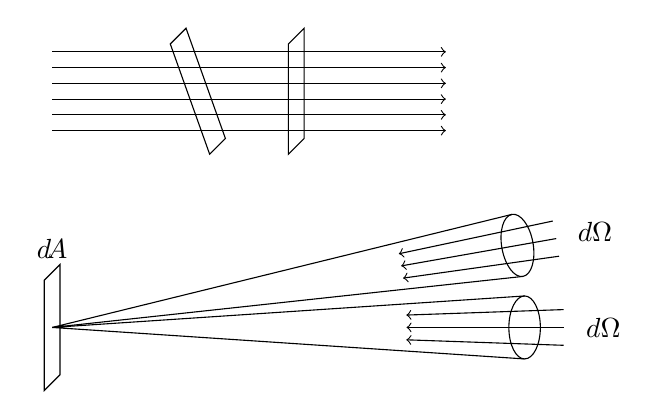
\begin{tikzpicture}
\begin{scope}[shift={(-6,-3)}]
\foreach \alpha in {0,10}  {
\begin{scope}[shift={(6,0)},rotate=\alpha]
\draw (6,0) ellipse (0.2 and 0.4);
\draw (6,0.4) -- (0,0) -- (6,-0.4);
\draw (7,0) node {$d \Omega$};
\foreach \ang in {-2,0,2} {
\draw [<-] (0,0) ++(\ang:4.5) -- ++(\ang:2);
}
\end{scope}
}
\draw (5.9,-0.8) -- (6.1,-0.6) -- (6.1,0.8) -- (5.9,0.6)  -- cycle ;
\draw (6,1) node {$d\!A$} ;
\end{scope}
\foreach \y in {-0.5,-0.3,...,0.5}  
{
\draw [->] (0,\y) -- (5,\y);
}
\draw (3,-0.8) -- (3.2,-0.6) -- (3.2,0.8) -- (3,0.6)  -- cycle ;
\draw (2,-0.8) -- (2.2,-0.6) -- (1.7,0.8) -- (1.5,0.6)  -- cycle ;

\end{tikzpicture}
\caption{Flux and intensity.  On the left the power delivered to the
  two surfaces are equal even though their areas differ.  The flux is
  the power per unit area so the tilted surface gets less flux.  On
  the right intensity is the power delivered to an area from a
  particular part of the sky (solid angle).  Here the two intensities
  are equal but the upper set of rays delivers less flux.}
\end{figure}
\section{Intensity}
\label{sec:intensity}
\index{radiation!intensity}

Although the flux is a useful quantity, it cannot encapsulate all of
our knowledge about a radiation field.  For example, one could shine a
faint light directly through a window or a bright light through the
same surface at an angle.  Both of these sitautions are characterized
by the same rate of energy flow through the surface, but they are
clearly different physical situations.

A more generally useful quantity quantifies the rate that energy flows
through a surface in a particular direction (imagine that the window
now looks into a long pipe so that only light travelling in a
particular direction can pass through,
\begin{equation}
dE = I d\!A d \Omega dt 
\label{eq:4}
\end{equation}
where $I$ is the intensity. Although this quantity seems a bit kludgy,
it is actually quite familiar.  It is the brightness.

You look at a light bulb.   As you move away from the light bulb, your
eye receives less flux ($F$ decreases) and the apparent size of the
light bulb also decreases ($d\Omega$ decreases).  It turns out that
these two quantities both decrease as $R^{-2}$, so the intensity or
brightness is conserved along a ray.  This result makes the intensity
a terrifically useful quantity.

\subsection{Relation to the flux}
\label{sec:relation-flux}

From the example at the beginning of this section we can deduce the 
relationship between the flux and the intensity of the light.
Radiation that travels perpendicular to a surface delivers more energy to 
that surface than radiation travelling at an angle.   You can always
imagine second surface perpendicular to the light ray through which all of
the energy that reaches the first surface travels.  We know that
intensity is the same along the ray so
\begin{equation}
d E = I d\!A_1 d \Omega d t= I d\!A_2 d \Omega d t
\label{eq:5}
\end{equation}
and $d\!A_2 = \cos \theta d\!A_1$, so the total flux travelling through
the surface is given by a moment of the intensity
\begin{equation}
F = \int I \cos \theta d \Omega
\label{eq:6}
\end{equation}
If $I$ is constant with respect to angle, there is as much energy
travelling from left to right as from right to left, so the net flux
vanishes, or more mathematically the mean of $\cos \theta$ vanishes 
over the sphere.

\paragraph{Something to think about}   The Sun is equally intense in
the summer and winter (if you exclude the effects of the
atmosphere), then why are winters colder than summers?   

A closely related quantity is the pressure that a radiation field
exerts on a surface.  Pressure is the rate that momentum is delivered 
to a surface in the direction perpendicular to the surface.  The
momentum of light is $E/c$ and the rate that energy is 
delivered to a surface from light travelling around a particular
direction is simply $I \cos \theta d\Omega$.  The component 
of the momentum that is directed perpendicular to the surface 
is $E \cos\theta/c$, so there is a second factor of $\cos \theta$ 
yielding the following integral.
\begin{equation}
p = \frac{1}{c} \int I \cos^2 \theta d \Omega.
\label{eq:7}
\end{equation}

\paragraph{Something to think about}  Does the radiation pressure 
from an isotropic radiation field vanish?

\subsection{Spectra}
\label{sec:spectra}

The quantities that we have defined so far can be examined as a
function of the frequency or wavelength of the radiation or the energy
of the individual photons, yielding $F_\nu, F_E, F_\lambda$ and 
also for the intensity, {\em e.g}
\begin{equation}
d E = F_{\nu} d \nu d\!A d t
\label{eq:8}
\end{equation}
and $F_\nu$ is called the specific flux.
The use of $F_{\nu}$ is so common that astronomers have a special 
unit to measure $F_\nu$
\begin{equation}
1~\hbox{\rm Jansky} = 1~\hbox{\rm Jy} = 10^{-26} \hbox{W m}^{-2}
\hbox{Hz}^{-1} = 10^{-23} \hbox{\rm erg cm}^{-1} \hbox{s}^{-1} \hbox{Hz}^{-1}.
\label{eq:9}
\end{equation}
This unit is most commonly used in the radio and infrared, and sometimes
in the x-rays.

A common combination that people use is 
\begin{equation}
E F_E = \lambda F_\lambda = \nu F_\nu  = \nu \frac{d F}{d \nu} =
\frac{d F}{d \ln \nu}.
\label{eq:10}
\end{equation}
This allows you to convert between $F_\nu$ and $F_\lambda$ etc.  And
it also gives the flux per logarithmic interval in photon energy or
frequency.  This is really handy since astronomers like to use log-log
plots.   A spectrum that goes as $F_\nu \propto 1/\nu$ has a constant 
amount of energy per logarithmic interval.

\paragraph{Something to think about}
A source emits at 1 Jansky from 100~MHz to 1~GHz and at 1 $\mu$Jy from
1 to 10 keV.  Is it brighter in the radio or x-rays?

\subsection{An Astronomical Aside: Magnitudes}
\label{sec:an-astr-asid}
\index{radiation!magnitudes}

Astronomers typically speak about the flux of an object in terms of 
magnitudes.   A magnitude is generally defined as
\begin{equation}
m = -2.5 \log_{10} \int_0^\infty g(\nu) F_{\nu,\Omega} d \nu + m_0.
\label{eq:11}
\end{equation}
What are the different quantities in this expression?  Pogson
empirically determined the value of ``2.5'' by comparing the
magnitudes of prominent observers of the 1800's.   It is remarkably close
to $\ln 10 \approx 2.3$, so a change in magnitude of 0.1 is about a 
ten-percent change in flux.

Another term in the expression is $g(\nu)$, the filter function that
determines which part of the electromagnetic spectrum you're are
looking at.  If $g(\nu)=1$, the quantity is called a ``bolometric
magnitude.''\index{radiation!bolometric magnitude}\index{bolometric
  magnitude}.  It is supposed to quantify the total energy coming from
the source.  One also hears about a quantity called the ``bolometric
correction''\index{bolometric correction} which is simply the
difference between the magnitude of source for a particular filter
($g(\nu)$) and for $g(\nu)=1$.

$F(\nu,\Omega)$ is the flux coming from the source as a function of
frequency integrated over a certain area of sky, $\Omega$.  For a star
one generally can extrapolate the flux that one observes in the sky to
the total flux, but the intensity from a galaxy or other extended
source generally falls off gradually so one defines a magnitude within
a certain aperture or down to a limiting intensity (surface
brightness).   

The final term is $m_0$, the zero point.  The value of the zero point
is a matter of convention.  Two of the standard conventions are the
``Vega'' convention which states that the magnitude of the star Vega
regardless of the function $g(\nu)$ is zero; all of Vega's colours are
zero.  This works nicely because you could always in principle observe
Vega with your equipment.

There are two problems however.  One is that the flux from Vega like
that of most stars varies a bit.  The second is that an object with a
flat spectrum (equal energies in each frequency interval) will have an
awkward set of colours (the difference in magnitudes for two different
$g(\nu)$ functions).  This leads to the second convention, the AB
system.
\begin{equation}
m(AB) = -2.5 \log_{10} f_\nu - 48.60 = -2.5 \log_{10} \left (
\frac{f_\nu}{1~\hbox{\rm Jy}}\right ) + 8.90
\label{eq:12}
\end{equation}
where $f_\nu$ is the flux in c.g.s. units.  The constants ``8.90'' 
and ``-48.60'' mean that $m(AB)=V$ for a flat spectrum source.

\paragraph{Something to think about}
How do you define an AB magnitude using a filter?

A final quantity that astronomers talk about is the surface
brightness.  This is just the intensity that we have been speaking
about all along.  However, the conventional nomenclature is rather strange,
magnitudes per square arcsecond.

\paragraph{Something to think about}
What is the magnitude of a source that subtends 10 square arcseconds
with a surface brightness of 19 magnitudes per square arcsecond?

\section{Energy Density}
\label{sec:energy-density}
\index{radiation!energy density}
Let's imagine that light is travelling through a small box.  How much
energy is in the box at any time?  First it is easiest to think about
how much energy in the box is travelling in a particular direction
through the box during a small time interval such that $c dt$ is the
length of the box,
\begin{equation}
d E = u(\Omega) d\!A c d t d\Omega
\label{eq:13}
\end{equation}
This energy equals the energy that enters the box travelling in the 
right direction during the time interval $dt$,
\begin{equation}
d E = I d\!A d t d\Omega
\label{eq:14}
\end{equation}
so
\begin{equation}
c u(\Omega) = I.
\label{eq:15}
\end{equation}
To get the total energy density you have to integrate over all of the 
ray directions
\begin{equation}
u = \frac{1}{c} \int I d \Omega = 4\pi \frac{J}{c}
\label{eq:16}
\end{equation}
where $J$ is the mean intensity.   Notice how it differs from the flux
defined earlier.

Let's revisit the radiation pressure formula.   But let's assume that
the radiation field is isotropic, so $I=J$ for all directions, we get
\index{radiation!pressure}
\begin{eqnarray}
\label{eq:17}
p &=& \frac{1}{c} \int J \cos^2\theta d \Omega \\
\label{eq:18}
  &=& \frac{1}{c} \int_0^\pi \int_0^{2\pi}J \cos^2\theta \sin\theta d\theta d \phi \\
  &=& \frac{1}{c} J \left ( 2 \pi \left . \frac{1}{3} \cos^3\theta \right |_0^\pi
  \right ) = \frac{4}{3} \pi \frac{J}{c} = \frac{1}{3} u.
\label{eq:19}
\end{eqnarray}

\subsection[A Physical Aside: Intensity and Flux]{A Physical Aside: What are the Intensity and Flux?}
\label{sec:physical-aside:-what}

How do the intensity and flux fit in with more familiar concepts like 
the flux of a vector field?   They really don't.   

One can define the flux in three perpendicular directions by asking
how much energy flows through three mutually perpendicular planes.
This flux vector transforms like a vector under rotations, but it
doesn't transform like a four-vector under boosts.  The flux vector
fills in the time-space components of the stress-energy tensor of the
electromagnetic field.  We have also calculated the time-time component which
is the energy density and the space-space components, the pressure.
To calculate how the flux transforms with respect to a boost (or
Lorentz transformation) by transforming the entire tensor.

The intensity ($I_\nu$) as we shall soon see is simply related to the
phase-space density of the ensemble of photons.

\section{Blackbody Radiation}
\label{sec:blackbody-radiation}
\index{radiation!blackbody}
\index{blackbody|see{radiation, blackbody}}
Blackbody radiation is a radiation field that is in thermal
equilibrium with itself.  In general we will find it convenient to
think about radiation that is in equilibrium with some material or its
enclosure.  Using detailed balance between two enclosures in
equilibrium with each other and the enclosed radiation we can quickly
derive several important properties of blackbody radiation.
\begin{itemize}
\item The intensity ($I_\nu$) of blackbody radiation does not depend on the
shape, size or contents of the enclosure.
\item Blackbody radiation is isotropic.
\end{itemize}
What remains is the temperature and the frequency.   Because the
intensity is a universal function of $T$ and $\nu$, we have
\begin{equation}
\hbox{\rm Kirchhoff's Law:}~~~~I_\nu = B_\nu (T)  \hbox{\rm ~for a blackbody at temperature~} T.
\label{eq:20}
\end{equation}
\index{Kirchhoff's Law}
Because heat flows from a hotter system to a cooler system we know 
that if $T_1 > T_2$, $B_\nu (T_1)>B_\nu(T_2)$ for all values of $\nu$.
To see this, imagine a filter that only lets light pass over a narrow
range of frequencies in the hole between the enclosures.  If this
condition did not hold, one could have energy flowing from the cooler
to the hotter enclosure.

\subsection{Thermodynamics}
\label{sec:thermodynamics}
\index{radiation!blackbody!thermodynamics}

The blackbody radiation in its enclosure is a system in equilibrium 
so we can use the equations of thermodynamics to glean some more of
its properties.  If we deliver some heat $dQ$ to the blackbody, it 
can change the internal energy of the blackbody $dU$ or do work $p
dV$.  The heat delivered also equals the change in entropy of the system
times the temperature of the system.
\begin{equation}
d Q = T d S = d U + p d V.
\label{eq:21}
\end{equation}
Now $U$ is simply the energy density times the volume of the enclosure
so $d U = u d V + V du/dT dT$ and we showed the $p=u/3$.   Let's put
this together
\begin{equation}
T d S = u d V + V \frac{d u}{d T} d T + \frac{1}{3} u d V.
\label{eq:22}
\end{equation}
If we rearrange and solve for the derivatives we get
\begin{equation}
\left ( \frac{\partial S}{\partial T} \right )_V = \frac{V}{T} \frac{d
u}{d T} ~~~~~~
\left ( \frac{\partial S}{\partial V} \right )_T = \frac{4}{3} \frac{u}{T}
\label{eq:23}
\end{equation}
Let's take the partial derivative of the first expression with respect
to $V$ and the second expression with respect to $T$ and set them
equal
\begin{equation}
\frac{1}{T} \frac{d u}{d T}  = \frac{4}{3} \frac{1}{T} \frac{d u}{d T}
- \frac{4}{3} \frac{u}{T^2}
\label{eq:24}
\end{equation}
Let's solve for $du/dT$ to get
\begin{equation}
\frac{d u}{d T} = \frac{4 u}{T}
\label{eq:25}
\end{equation}
so 
\begin{equation}
\hbox{\rm Stefan-Boltzmann Law:}~~~~u = a T^4
\label{eq:790}
\end{equation}
where $a$ is a constant of integration.  The value of $a$ is 
$7.56 \times 10^{15}$~erg~cm$^{-3}$K$^4$.
\index{Stefan-Boltzmann  Law}

\paragraph{Something to think about} Why does $du/dV$ vanish?

We found that for an isotropic radiation field the energy density is 
simply related to the intensity, $u = 4\pi J/c$.  For a blackbody
$J=B(T)$ so we have
\begin{equation}
B(T) = \frac{a c}{4\pi} T^4.
\label{eq:26}
\end{equation}
Let's imagine that our blackbody enclosure has a small hole of area
$d\!A$ in it. How much energy emerges through this hole
\begin{equation}
F d\!A = \int_{\hbox{\rm \scriptsize out}} \cos\theta B(T) d \Omega
 = B(T) \int_0^{\pi/2} \int_0^{2\pi} \cos\theta \sin\theta d\theta d\phi =
 \pi B(T).
\label{eq:27}
\end{equation}
We write this more compactly by defining $\sigma=ac/4$ so we have
\begin{equation}
\hbox{\rm Another Stefan-Boltzmann Law:}~~~~F=\sigma T^4
\label{eq:793}
\end{equation}
where $\sigma = 5.67 \times
10^{-5}$~erg~cm$^{-2}$s$^{-1}$K$^{-4}$. 

Using the earlier results we can also derive the entropy of the 
radiation field
\begin{equation}
S = \frac{4}{3} a T^3 V.
\label{eq:28}
\end{equation}

\subsection{Statistical Mechanics}
\label{sec:stat-mech}
\index{radiation!blackbody!statistical mechanics}

We have managed to derive several interesting properties of blackbody
radiation but we still have no idea what its spectrum is.  To figure
this out we have to think about the microscopic properties of the
radiation field.  Let's imagine that we have blackbody radiation in a
box whose wavenumber $k_x$ ranges from $k_x$ to $k_x + dk$.  How many
different types of waves lie in this interval?

You may be tempted to say as many as you want, but the waves are
trapped in a box.  Let's say that the box has length $l_x$ in the
$x$-direction; therefore, $k_x l_x = 2 \pi n_x$ where $n_x$ is an
integer so that the radiation field has a node at the edges of the
box, so between $k_x$ and $k_x + dk$ there are only $2 dk l_x / (2\pi)$
different states.  The factor of two arises because the waves have two
independent polarization states.   If we imagine a small cube in phase
space of size $d k_x d k_y d k_z$ we get 
\begin{equation}
d N = 2 \frac{l_x l_y l_z }{(2\pi)^3} d^3 k = 2 \frac{d V}{(2\pi)^3} d^3 k.
\label{eq:29}
\end{equation}
Now we have $d^3 k = k^2 dk d \Omega$ and $k=2\pi \nu/c$ so
\begin{equation}
d^3 k = d \nu d\Omega \frac{(2\pi)^3}{c^3} \nu^2
\label{eq:30}
\end{equation}
We find that the density of states is given by
\begin{equation}
\rho_s \equiv \frac{d N}{d V d\Omega d \nu} = \frac{2 \nu^2}{c^3}
\label{eq:31}
\end{equation}
The energy density ($u_\nu(\Omega)$)of the radiation field is simply the density of
states times the mean energy per state and $c u_\nu(\Omega)=I_\nu$.

Classically we find that the mean energy per state is simply given by 
$k T$.  Let's try this out for size,
\begin{equation}
u^{\hbox{\rm \scriptsize classical}}_\nu (\Omega) = \frac{2\nu^2}{c^3} k T.
\label{eq:32}
\end{equation}
This is the great Rayleigh-Jeans law and it actually works pretty
well, unless you look at large frequencies and find that the total
energy $B(T)$ is infinite.  This is called the Rayleigh-Jeans (or
ultraviolet) catastrophe.

The solution to this problem ushered in the era of modern physics.
Planck argued that if light comes in discrete packages (photons) whose
energy is proportional to the frequency we can solve this problem
($E=h\nu$).  Let's try a really simple minded approach to assume that
only photons with $E<kT$ are in the radiation field then we have
\begin{equation}
u^{\hbox{\rm \scriptsize classical fixed?}}_\nu(\Omega) = 
\left \{ \begin{array}{ll}
	\frac{2\nu^2}{c^3} k T & h \nu < k T \\
	0 & h \nu \geq k T 
	\end{array}
\right .
\label{eq:33}
\end{equation}
Let's integrate $u_\nu$ over the frequency range and solid angle to get
\begin{equation}
u^{\hbox{\rm \scriptsize classical fixed?}} = 
\frac{8\pi k T }{3 c^3} \left ( \frac{k T}{h} \right )^3
= \frac{8 \pi k^4}{3 c^3 h^3} T^4.
\label{eq:34}
\end{equation}
This has the right behaviour and the numerical constant differs from
the actual value by a factor of about 20.

It turns out that we can do a whole lot better.   According to
statistical mechanics the probability of a state of energy $E$ is
proportional to $e^{-\beta E}$ where $\beta = 1/(k T)$.  The energy 
in a particular state is proportional to the number of photons 
in the state $E_n=n h\nu$.  The mean energy in a state is given
by 
\begin{equation}
{\bar E} = \frac{\sum_{n=0}^\infty E_n e^{-\beta E_n}}
{\sum_{n=0}^\infty e^{-\beta E_n}}
\label{eq:35}
\end{equation}
Notice that the expression on the top is the derivative of the
expression on the bottom with respect to $\beta$, so we find
\begin{equation}
{\bar E} = -\frac{\partial}{\partial \beta} \ln \left (
\sum_{n=0}^\infty e^{-\beta E_n} \right ).
\label{eq:36}
\end{equation}
We haven't assumed anything about the states themselves yet, so this
result would apply for any system.   Here we know that $E_n = n h \nu$
so
\begin{equation}
\sum_{n=0}^\infty e^{-\beta E_n}  =
\sum_{n=0}^\infty r^n  = \frac{1}{1-r} = \frac{1}{1-e^{-\beta h \nu}}
\label{eq:37}
\end{equation}
so
\begin{equation}
{\bar E} = \frac{h \nu}{e^{\beta h \nu} - 1}
\label{eq:38}
\end{equation}
For $h \nu \ll\ k T$ $\beta h \nu \ll\ 1$ so we have
\begin{equation}
{\bar E} \approx \frac{h \nu}{1 + \beta h \nu - 1} = \frac{h
\nu}{\beta h \nu} = k T,
\label{eq:39}
\end{equation}
the classical result.  But for $h \nu \gg\ k T$ we have 
$\beta h \nu \gg\ 1$
\begin{equation}
{\bar E} \approx h \nu\exp(-\beta h \nu ).
\label{eq:40}
\end{equation}
If we use this value with the density of states we get the Wien law.

Let's derive the expression for the spectrum for all frequencies.
We have the value of energy density
\begin{equation}
u_\nu(\Omega) = \frac{2 h}{c^3} \frac{\nu^3}{\exp ( h \nu / k T) - 1}
\label{eq:41}
\end{equation}
so that
\begin{equation}
\hbox{\rm Planck's Law:}~~~~B_\nu (T) = \frac{2 h}{c^2} \frac{\nu^3}{\exp ( h \nu / k T) - 1}.
\label{eq:42}
\end{equation}
\index{Planck's Law}
Wien's displacement law gives the frequency of the 
peak of the blackbody curve $B_\nu$
\begin{equation}
h \nu_\mathrm{max} \approx 2.821439 k T 
\label{eq:794}
\end{equation}
\index{Wien's displacement law}
or $\nu_\mathrm{max}=58.79 T~\mathrm{GHz/K}$.

\paragraph{Something to think about}  At what energy does the flux per
logarithmic energy interval reach its peak? How about flux per unit wavelength?

Let's try to find the value of $a$, the constant in the
Stefan-Boltzmann Law.  First we have 
\begin{equation}
u_\nu = 4 \pi u_\nu(\Omega) = \frac{8 \pi h}{c^3} \frac{\nu^3}{\exp ( h \nu / k T) - 1}.
\label{eq:43}
\end{equation}
The total energy density is $\int u_\nu d\nu$
\begin{equation}
u = \int_0^\infty \frac{8 \pi h}{c^3} \frac{\nu^3}{\exp ( h \nu / k T)
- 1} d \nu = \frac{8 \pi h}{c^3} \left ( \frac{kT}{h} \right )^4 
\int_0^\infty \frac{x^3}{e^x - 1} d x.
\label{eq:44}
\end{equation}
The integral can be evaluated using a Taylor series
\begin{equation}
\int_0^\infty \frac{x^3}{e^x - 1} d x
= \int_0^\infty \frac{x^3 e^{-x}}{1-e^{-x}} d x =
\int_0^\infty x^3 \sum_{n=1}^{\infty} e^{-nx} d x = \sum_{n=1}^\infty \frac{6}{n^4}
\label{eq:45}
\end{equation} 
to yield $\pi^4/15$ (see \S~\ref{sec:integral-b_nut} for further details),so
\begin{equation}
  u = a T^4~\hbox{\rm where}~a = \frac{8\pi^5}{15} \frac{k^4}{\left (h c \right)^3} =
  \frac{\pi^2}{15} \frac{k^4}{\left (\hbar c\right)^3}.
\label{eq:792}
\end{equation}
The number density of photons can be determined in a similar way but
the exponent in the integral is ``2'' instead of ``3'' yielding
\begin{equation}
n = \frac{16 \zeta(3) \pi k^3}{c^3 h^3} T^3
\end{equation}
so the mean energy per photon is given by
\begin{equation}
\frac{u}{n} = \frac{\pi^4}{30 \zeta(3)} k T \approx 2.701 k T.
\end{equation}
Coincidentally the numeric factor differs from $e$ by less than one
percent.

\subsection{Blackbody Temperatures}
\label{sec:blackb-temp}
\index{radiation!temperature}
A blackbody is of course characterized by a single temperature, $T$.
However, it is often convenient to characterize the radiation from
astrophysical sources by assuming that it is a blackbody and using
some property of the blackbody spectrum to derive a characteristic
temperature for the radiation.   There are three characteristic
temperatures in common usage: {\it brightness}
temperature,
{\it effective} temperature and the {\it colour} temperature.
\index{brightness temperature|see{temperature!brightness}}\index{effective temperature|see{temperature|effective}}\index{colour temperature|see{temperature!colour}}
\index{temperature!brightness}\index{temperature!effective}\index{temperature!colour}

The brightness temperature is determined by equating the brightness or 
intensity of an astrophysical source to the intensity of a blackbody
and solving for the temperature of the corresponding blackbody. 
\begin{equation}
I_\nu = B_\nu(T_b).
\label{eq:46}
\end{equation}
This expression is most useful in the regime where the intensity of
the blackbody is proportional to the temperature {\em i.e.} the
Rayleigh-Jeans limit.  Here we have,
\begin{equation}
T_b = \frac{c^2}{2\nu^2 k} I_\nu.
\label{eq:47}
\end{equation}
The brightness temperature has several nice properties. 
For one thing it has units of Kelvin rather than something
clumsy. Second if a material is emitting thermal radiation one can
obtain a simple expression of the radiative transfer equation 
(see the problems).

\paragraph{Something to think about} 
In what regime does the linear relationship between the brightness
temperature and the intensity begin to fail?  How can you tell?

The colour temperature is defined by looking at the peak of the
emission from the source and using Wien's displacement law to define a 
corresponding temperature.   This may be done in a more sophisicated
manner by fitting a blackbody spectrum or something like that.

Finally the effective temperature is the temperature of a blackbody
that emits the same flux at its surface as the source, {\em i.e.}
\begin{equation}
F = \sigma T_\mathrm{eff}^4
\label{eq:791}
\end{equation}

\section{Radiative Transfer}
\label{sec:radiative-transfer}
\index{radiative transfer}
As a ray passes through some material its intensity may increase or
decrease depending on the properties of the matter.  To understand
this process it is helpful to make some defintions.

\subsection{Emission}
\label{sec:emission}
\index{radiative transfer!emission}

Generally material has two routes for the emission of radiation:
stimulated emission and spontaneous emission.  The rate of the former
is proportion to the intensity of the beam so it is convenient to lump
it with the absorbing properties of the material.   The spontaneous
emission is independent of the radiation field.

\index{radiative transfer!sponaneous emission coefficent}
Let's define the {\em spontaneous emission coefficient}, $j$.  This is
the energy emitted per unit time into unit solid angle from a unit
volume, so we have
\begin{equation}
d E = j dV d\Omega dt
\label{eq:48}
\end{equation}
and similarly
\begin{equation}
d E = j_\nu dV d\Omega dt d\nu.
\label{eq:49}
\end{equation}
If the emitter is isotropic or the emitters are randomly oriented then
the total power emitted per unit volume and unit frequency is
\begin{equation}
P_\nu = 4\pi j_\nu.
\label{eq:50}
\end{equation}
Often the emission is isotropic and it is convenient to define the
emissivity of the material per unit mass
\begin{equation}
dE = \epsilon_\nu \rho dV dt d\nu \frac{\Omega}{4\pi}
\label{eq:51}
\end{equation}
where $\rho$ is the density of the emitting medium.  $\epsilon_\nu$ is
simply related to $j_\nu$ for an isotropic emitter
\begin{equation}
j_\nu = \frac{\epsilon_\nu \rho}{4\pi}.
\label{eq:52}
\end{equation}
As a beam travels through the material, its intensity increases such
that
\begin{equation}
\frac{d I_\nu}{ds} = j_\nu.
\label{eq:53}
\end{equation}
Here is the first term in the equation of radiative transfer.  We know
what $I_\nu$ is and we will spend much effort figuring out what
$j_\nu$ is for different physical systems.

\subsection{Absorption}
\label{sec:absorption}
\index{radiative transfer!absorption}

The equation for absorption is similar, except that amount of
absorption is proportional to the intensity of the radiation.  You
can't absorb radiation that isn't there.
\begin{equation}
\frac{d I_\nu}{ds} = -\alpha_\nu I_\nu.
\label{eq:54}
\end{equation}
Phenomenologically you can imagine that there are many independent
absorbers in the beam, each with a cross section $\sigma_\nu$ and a
number density $n$.  This would yield 
\begin{equation}
\alpha_\nu = \sigma_\nu n.
\label{eq:55}
\end{equation}
It is often convenient to define $\alpha_\nu = \rho \kappa_\nu$ where
$\kappa_\nu$ is the opacity of the material.  You can think of this as
the cross section per unit mass of the absorbers.

The quantity $\alpha_\nu$ has both positive and negative
contributions.  The positive contributions are {\em true absorption}  and
the negative ones correspond to {\em stimulated emission}.

\subsection{The Radiative Transfer Equation}
\label{sec:radi-transf-equat}
\index{radiative transfer!differential equation}

Putting these equations together yields the radiative transfer equation,
\begin{equation}
\frac{d I_\nu}{ds} = -\alpha_\nu I_\nu + j_\nu.
\label{eq:56}
\end{equation}
Once we know $\alpha_\nu$ and $j_\nu$ for the system of interest, it
is straightforward to solve the equations of radiative transfer.
We shall see a formal solution a bit later.  If there is scattering as
well as absorption and emission, things get a bit more complicated.

Let's look at a few examples. 
\begin{enumerate}
\item {\bf Emission only}
\begin{equation}
\frac{d I_\nu}{ds} = j_\nu
\label{eq:57}
\end{equation}
yields the solution
\begin{equation}
I_\nu (s) = I_\nu(s_0) + \int_{s_0}^s j_\nu (s') ds'
\label{eq:58}
\end{equation}
The increase in brightness is simply the integral of the emission
coefficient along the line of sight.  This limit is also know as the
{\em optically thin} regime (absorption can be neglected).
\item {\bf Absorption only}
\begin{equation}
\frac{d I_\nu}{ds} = - \alpha_\nu I_\nu 
\label{eq:59}
\end{equation}
which yields
\begin{equation}
I_\nu (s) = I_\nu(s_0) \exp \left [ -\int_{s_0}^s \alpha_\nu (s') ds'
  \right ]
\label{eq:60}
\end{equation}
The result for pure absorption inspires us to look at the radiative
transfer equation again. Let's define, the optical depth\index{optical
  depth},
\begin{equation}
\tau_\nu = \int_{s_0}^s \alpha_\nu (s') ds' 
\label{eq:61}
\end{equation}
such that $d\tau_\nu = \alpha_\nu ds$
\item {\bf Emission and absorption}
Using this defintion we get the following equation of radiative
trasnfer,
\begin{equation}
\frac{d I_\nu}{d\tau_\nu} = -I_\nu + S_\nu
\label{eq:62}
\end{equation}
where 
\begin{equation}
S_\nu \equiv \frac{j_\nu}{\alpha_\nu}
\label{eq:63}
\end{equation}
is called the {\em source function}.  It has the same units as the 
intensity.  It allows a formal solution of the transfer equation
\begin{equation} 
I_\nu (\tau_\nu) = I_\nu(s_0)e^{-\tau_\nu} + \int_0^{\tau_\nu}
e^{-(\tau_\nu - \tau_\nu')} S_\nu(\tau_\nu') d\tau_\nu'.
\label{eq:64}
\end{equation}
This expression makes a lot of sense.  The first term is the radiation
that we start with and attentuated through the medium.  The second
term is the sum of all the radiation emitted in the medium and
attentuated from where it is emitted until it escapes. If we have a
source with a constant value of $S_\nu$, the solution is much simpler
\begin{equation}
I_\nu (\tau_\nu) = I_\nu(s_0)e^{-\tau_\nu} + S_\nu \left ( 1 -
e^{-\tau_\nu} \right ) = S_\nu + e^{-\tau_\nu} \left ( I_\nu(0) - S_\nu
\right ).
\label{eq:65}
\end{equation}
The intensity field approaches the source function as the optical
depth increases.
\end{enumerate}

\section{Thermal Radiation}
\label{sec:thermal-radiation}
\index{radiation!thermal}
Let's imagine a blackbody enclosure, and we stick some material inside
the enclosure and wait until it reaches equilibrium with the radiation
field, $I_\nu = B_\nu(T)$.  Now let move the material in a position
the blocks our window to the enclosure. What can we say about the
source function of the material?

We know that as light travels through the material the intensity field
should approach the source function but we also know that the light
emerging from the window must have $I_\nu=B_\nu(T)$.  If it didn't, we
could set up an adjacent blackbody enclosure at the same temperature
and energy would flow between them.  We must conclude that
\begin{equation}
\hbox{Another Kirchoff's Law:}~~~~S_\nu = B_\nu(T) \hbox{\rm ~for a thermal emitter}
\label{eq:66}
\end{equation}
Furthermore, we can look at the transfer equation that yields,
\begin{equation}
\frac{d I_\nu}{d \tau_\nu} = -I_\nu + B_\nu(T).
\label{eq:67}
\end{equation}
Because $I_\nu=B_\nu(T)$ outside of the thermal emitting material and 
$S_\nu=B_\nu(T)$ within the material, we find that $I_\nu=B_\nu(T)$
throughout the enclosure.

If we remove the thermal emitter from the blackbody enclosure we can
see the difference between thermal radiation and blackbody radiation.
A thermal emitter has $S_\nu = B_\nu(T)$, so the radiation field
approaches $B_\nu(T)$ (blackbody radiation) only at large optical
depth.

\subsection{Einstein Coefficients}
\label{sec:einst-coeff}
\index{radiation!Einstein coefficients}

Kirchoff's law yields a relationship between the emission and absorption
coefficients for a thermally emitting material, specifically 
$j_\nu = \alpha_\nu B_\nu$.  This relationship suggests some
connection between emission and absorption at a microscopic level.  It
was Einstein that first elucidated this connection.

Let's imagine a two-level atom.  The lower level has energy $E$ and
statistical weight $g_1$.  You can think of the statistical weight as
the number of ways that the atom can be in the particular state, the
degeneracy of the state.  The second level has an energy $E+h\nu_0$
and a statistical weight of $g_2$.

There are three possible transitions,
\begin{enumerate}
\item {\rm Spontaneous Emission} with probability per unit time of
  $A_{21}$.
\item {\rm Absorption} with a rate proportional to the
  angle-averaged intensity of the radiation field ($J_\nu(\nu_0)$) times the
  coefficient $B_{12}$.  
  
  Technically the atom does not absorb at precisely one frequency
  but over a width $\delta \nu$.  To simplify matters we will take
  $\delta \nu \rightarrow 0$ and the line profile $\phi(\nu)
  \rightarrow \delta(\nu-\nu_0)$.
\item {\rm Stimulated Emission} with a transition rate of
  $B_{21} J_\nu(\nu_0)$.
\end{enumerate}

For the system to be in thermodynamic equilibrium, the number of
transitions from level one to two must equal the reverse transitions,
\begin{equation}
n_1 B_{12} J_\nu(\nu_0) = n_2 A_{21} + n_2 B_{21} J_\nu(\nu_0).
\label{eq:68}
\end{equation}
Let's solve for $J_\nu(\nu_0)$,
\begin{equation}
J_\nu(\nu_0) = \frac{n_2 A_{21}}{n_1 B_{12} - n_2 B_{21}}.
\label{eq:69}
\end{equation}
We know that the system is in thermodynamic equilibrium so 
\begin{equation}
\frac{n_1}{n_2} = \frac{g_1 \exp(-E/kT)}{g_2 \exp (-(E+h\nu_0)/kT)} =
\frac{g_1}{g_2} \exp (h\nu_0/kT).
\label{eq:70}
\end{equation}
Let's substitute this into the earlier result
\begin{equation}
J_\nu(\nu_0) = \frac{ A_{21}}{ (g_1/g_2) \exp(h\nu_0/kT) B_{12} - B_{21}}
\label{eq:71}
\end{equation}        
We know that since the system is in thermodynamic equilibrium with the
radiation field $J_\nu=B_\nu(T)$ 
\begin{eqnarray}
\frac{2 h}{c^2} \frac{\nu^3}{\exp ( h \nu_0 / k T) - 1}. &=& \frac{
  A_{21}}{ (g_1/g_2) \exp(h\nu_0/kT) B_{12} - B_{21}} \\
                                                        &=&
  \frac{A_{21}}{B_{21}} \frac{1}{(g_1/g_2) \exp(h\nu_0/kT) B_{12}/B_{21} - 1} .
\label{eq:72}
\end{eqnarray}
Because the temperature $T$ may be set arbitrarily we must have the
following relationships
\begin{eqnarray}
\label{eq:73}
A_{21} &=& \frac{2h\nu^3}{c^2} B_{21},\\
g_1 B_{12} &=& g_2 B_{21}.
\label{eq:74}
\end{eqnarray}
Because the Einstein coefficients are properties of the atom alone,
they do not depend on the assumption of thermodynamic equilibrium.
They are quite powerful.  If we calculate the probability of
absorption of a photon for example, we can use the Einstein relations
to find the rate of stimulated and spontaneous emission.   This proof
is an example of the principle of {\em detailed balance} of a
microscopic process.  

\paragraph{Something to think about}  Can you use the principle of
detailed balance to say anything about the relationship between the
stimulating and the stimulated photon?

\subsection[A Physical Aside: Einstein coefficients]{A Physical Aside: What is deep about the Einstein coefficients?}
\label{sec:physical-aside:-what-1}

The Einstein coefficients seem to say something magical about the properties
of atoms, electrons and photons.   Somehow atoms are forced to behave
according to these equations.  It turns out that the relationships between 
Einstein coefficients (1917) are an example of Fermi's Golden Rule
(late 1920s).  Fermi's Golden Rule relates the cross-section for a
process to a quantum mechanical matrix element and the phase space
available for the products.  Because quantum mechanics for the most
part is time reversible, the cross-section for the forward and reverse
reactions are related.

\section{Calculating the Emission and Absorption Coefficients}
\label{sec:calc-emiss-absoprt}

We can write the emission and absorption coefficients in terms of the
Einstein coefficients that we have just exmained.  The emission
coefficient $j_\nu$ has units of energy per unit time per unit volume
per unit frequency per unit solid angle!  The Einstein coefficient
$A_{21}$ gives spontaneous emission rate per atom, so dimensional analysis
quickly gives
\begin{equation}
j_\nu = \frac{h \nu}{4\pi} n_2 A_{21} \phi(\nu)
\label{eq:75}
\end{equation}
The absorption coefficent may be constructed in a similar manner
\begin{equation}
\alpha_\nu = \frac{h \nu}{4\pi} \phi(\nu) \left (n_1 B_{12} - n_2 B_{21} 
\right )
\label{eq:76}
\end{equation}
We can now write the absorption coefficient and the source function using the 
relationships between the Einstein coefficients as 
\begin{eqnarray}
\label{eq:77}
\alpha_\nu &=& \frac{h\nu}{4\pi} n_1 B_{12} \left ( 1 - \frac{g_1
n_2}{g_2 n_1}\right ) \phi(\nu) 
\label{eq:839}\\ 
S_\nu &=& \frac{2h\nu^3}{c^2} \left (
\frac{g_2 n_1}{g_1 n_2} - 1 \right )^{-1}.
\label{eq:78}
\end{eqnarray}

\subsection{LTE}
\label{sec:lte}
\index{radiative transfer!LTE}
To derive these relations we have not made any assumptions about
whether the photons or the matter are in thermal equilibrium with
themselves or each other.  An extremely useful assumption is that the
matter is in thermal equilibrium at least locally (Local Thermodynamic
Equilibrium).  This assumption forms the basis of the theory of stellar
atmospheres.

In this case the ratio of the number of atoms in the various states is
determined by the condition of thermodynamic equilibrium
\begin{equation}
\frac{n_1}{n_2} = \frac{g_1}{g_2} \exp \left (\frac{h\nu_0}{kT}\right).
\label{eq:79}
\end{equation}
This ratio yields the following absorption coefficient and source
function
\begin{eqnarray}
\label{eq:80}
\alpha_\nu &=& \frac{h\nu}{4\pi} n_1 B_{12} \left [ 1 - \exp
\left (-\frac{h\nu_0}{kT} \right ) \right] \\
S_\nu &=& B_\nu(T)
\label{eq:81}
\end{eqnarray}

\paragraph{Something to think about}  Because the source function
equals the blackbody function, does this mean that sources in local
thermodynamic equilibrium emit blackbody radiation?

\subsection{Non-Thermal Emission}
\label{sec:non-thermal-emission}
\index{radiation!non-thermal}
In any situation where 
\begin{equation}
\frac{n_1}{n_2} \neq \frac{g_1}{g_2} \exp \left (\frac{h\nu_0}{kT}\right).
\label{eq:82}
\end{equation}
(\ie if the radiating particles do not have a Maxwellian distribution)
one has to use the full expression for the source function; a
power-law distibution oftens occurs astrophysically.

An extreme example of non-thermal emission is the maser.   For atoms
in thermodynamic equilibrium we have
\begin{equation}
\frac{n_2 g_1}{n_1 g_2} = \exp \left (-\frac{h\nu}{kT} \right ) < 1
\label{eq:83}
\end{equation}
so that 
\begin{equation}
\frac{n_1}{g_1} > \frac{n_2}{g_2}
\label{eq:84}
\end{equation}
which means that the absorption coefficient is always positive in
thermodynamic equilibrium.  However, let us imagine a situation in
which
\begin{equation}
\frac{n_1}{g_1} < \frac{n_2}{g_2}.
\label{eq:85}
\end{equation}
This yields a negative absorption coefficient, so the optical depth
decreases and becomes negative as one passes through a region with
inverted populations and the intensity of the radiation actually
increases expontentially as the magnitude of the optical depth
increases.  So we have to thank Einstein for the laser as well.

\section{Scattering}
\label{sec:scattering}
\index{radiative transfer!scattering}

From the preceding discussion one might think that the theory of
radiative transfer simply relies on the application of the formal
solution using the Einstein coefficients for various processes of
interest.   

However, there is a big elephant in the middle of the room that we
have been ignoring --- {\bf scattering}.  Why is scattering a problem?
Couldn't you think about scattering as the absorption and re-emission
of a photon and include the process in the absorption coefficients and
source functions?  The answer is no.

The formalism that we have developed so far doesn't allow there to be
a correlation between the properties of an absorbed photon and the
emitted photon.  On the other hand, the initial direction and energy
of a scattered photon are generally highly correlated with the
photon's final momentum.  

We can first look at a process in which the photon is scattered into
a random direction without a change in energy.  This yields an
emission coefficient of 
\begin{equation}
j_\nu = \sigma_\nu J_\nu.
\label{eq:86}
\end{equation}
Notice that the emission rate depends on the radiation field through
$J_\nu$ and not solely on the properties of the scatterer through
$\sigma_\nu$.  If isotropic scattering is the only process acting we
find that the source function
\begin{equation}
S_\nu = J_\nu = \frac{1}{4\pi} \int d\Omega I_\nu.
\label{eq:87}
\end{equation}
The equation describing the evolution of the radiation field is still
rather innocuous looking 
\begin{equation}
\frac{d I_\nu}{ds} = -\sigma_\nu \left ( I_\nu - J_\nu \right ).
\label{eq:88}
\end{equation}
However, it is a completely different beast.  The evolution of the
intensity of a particular ray depends not only the intensity of the
ray and the local properties of the material but also on the intensity
of all other rays passing through the same point --- we have an 
{\bf integro-differential equation}.

If you think about things more generally, we had this same problem
before introducing scattering because the properties of the emitting
and absorbing material usually depend on the radiation field.  Even if
one neglects scattering, one often has to solve an
integro-differential equation.

\subsection{Random Walks}
\label{sec:random-walks}
\index{radiative transfer!random walks}
We can get an order of magnitude feeling for how much scattering will
affect the radiation field emerging from a source using the concepts
of the mean free path and the random walk.

The mean free path for scattering (or similarly for absorption) is
simply the reciprocal of the scattering coefficient $\sigma_\nu$.  So
if we imagine a single photon travelling through the material, it will
go typically a distance $l=\sigma_\nu^{-1}$ then change direction.  The
net displacement of the photon after $N$ free paths is
\begin{equation}
{\bf R} = {\bf r}_1 + {\bf r}_2 + {\bf r}_3 + \cdots + {\bf r}_N.
\label{eq:89}
\end{equation}
However, on average it is as likely to go one way as the other so the
mean values of all of the ${\bf r}_i$ vectors vanishes as does the
sum.   Let's ask instead how far the photon typically ends up away
from the starting point, here we have
\begin{eqnarray}
|{\bf R}|^2 &=& |{\bf r}_1|^2 + |{\bf r}_2|^2 + |{\bf r}_3|^2 + \cdots
+ |{\bf r}_N|^2 \\
 & & ~~~  + 2 {\bf r_1}\cdot {\bf r_2} + 2 {\bf r_1}\cdot {\bf r_3} + \cdots
\label{eq:90}
\end{eqnarray}
All of the cross terms vanish on average if the scattering is
isotropic, but $\left <{bf r_1}^2 \right > \approx l = \sigma_\nu^{-1}$ so the net
distance travelled after $N$ scatterings is
\begin{equation}
l_*^2 = N l^2, l_* = \sqrt{N} l.
\label{eq:91}
\end{equation}
If some blob of gas has a typically dimension $L$ we can estimate the
number of scatterings through the gas to be $N \approx L^2/l^2$.  This
is why people sometimes say that it takes a million years for a photon
to escape the sun.

In general if $\tau$ is large the average number of scatterings $N
\approx \tau^2$ while for $\tau \ll\ 1$, $N\approx \tau$

\subsection{Combined Scattering and Absorption}
\label{sec:comb-scatt-absorpt}
\index{radiative transfer!scattering and absorption}

In general a material can both scatter and absorb photons.  In this
case the transfer equation has two terms.  Let's focus on coherent
isotropic scattering and thermal emission and get
\begin{eqnarray}
\label{eq:92}
\frac{dI_\nu}{ds} &=& -\alpha_\nu \left (I_\nu - B_\nu \right ) -
\sigma_\nu \left (I_\nu - J_\nu \right ) \\
&=& -\left (\alpha_\nu + \sigma_\nu \right ) \left ( I_\nu - S_\nu
\right )
\label{eq:93}
\end{eqnarray}
where
\begin{equation}
S_\nu = \frac{\alpha_\nu B_\nu + \sigma_\nu J_\nu}{\alpha_\nu + \sigma_\nu}
\label{eq:94}
\end{equation}
The net absorption coefficient is $\alpha_\nu+\sigma_\nu.$ On average
a photon will travel a distance 
\begin{equation}
l_\nu = \frac{1}{\alpha_\nu + \sigma_\nu}
\label{eq:95}
\end{equation}
before it is absorbed or scattered.  The chance that the free path
will end in absorption is 
\begin{equation}
\epsilon_\nu = \frac{\alpha_\nu}{\alpha_\nu + \sigma_\nu}
\label{eq:96}
\end{equation}
and the chance that it will be scattered is 
\begin{equation}
1-\epsilon_\nu = \frac{\sigma_\nu}{\alpha_\nu + \sigma_\nu}.
\label{eq:97}
\end{equation}
We can rewrite the source function as
\begin{equation}
S_\nu = \left ( 1 - \epsilon_\nu \right ) J_\nu + \epsilon_\nu B_\nu.
\label{eq:98}
\end{equation}
After a photon is emitted it may bounce around several times before it
is absorbed; the average number of scatterings per absorption is 
$N=\epsilon_\nu^{-1}$.   After these $N$ scatterings it will typically
have travelled a distance,
\begin{equation}
l_* = \sqrt{N} l = \frac{1}{\sqrt{\alpha_\nu (\alpha_\nu+\sigma_\nu)}} 
\label{eq:99}
\end{equation}
$l_*$ is the typically distance between the points of creation and
destruction of a photon -- it is called the {\em diffusion length},
{\em the thermalization length}, or the {\em effective mean free
  path}.   If the material has some thickness $L$, we can define the
{\em effective optical depth} of the material to be 
$\tau_* = L/l_*$.

If $\tau_*$ is small, then a photon after being created in the medium,
bounces around until it emerges (it is usually not absorbed).  In this
case the power emitted by material will simply be 
\begin{equation}
{\cal L}_\nu = 4\pi \alpha_\nu B_\nu V, ~~~ (\tau_* \ll 1)
\label{eq:100}
\end{equation}
where $B_\nu$ is the source function (a blackbody for thermal
emission) without scattering and $V$ is the
volume of the material.  If $\tau_* \ll 1$ the material is said to be
{\em effectively thin} or {\em translucent}.

On the other hand, if $\tau_* \gg 1$, the medium is said to be 
{\em effectively thick}.  In this case only photons emitted within
$l_*$ of the surface typically escape without being absorbed.  We can
estimate the power emitted by
\begin{equation}
{\cal L}_\nu = 4\pi \alpha_\nu B_\nu A l_* = 
4\pi \sqrt{\epsilon_\nu} B_\nu A, ~~~ (\tau_* \gg 1)
\label{eq:101}
\end{equation}

\section{Radiative Diffusion} 
\label{sec:radiative-diffusion}
\index{radiative transfer!diffusion}
We have used the random walk arguments to show that the radiation
field approaches a blackbody within a few effective mean paths (or
thermalization lengths) of the surface.  Furthermore, the radiation
field becomes isotropic within a mean free path of the surface.  We
will first look at the first situation in which the radiation field is
approximately a blackbody.

\subsection{Rosseland Approximation}
\label{sec:ross-appr}
\index{radiative transfer!Rosseland approximation}
Because stellar atmospheres (i.e. the effective mean path) are
generally thin compared to the size of the star, we can assume that
this region has plane parallel symmetry; that is, the properties
of the material depend only on the depth from the surface $z$.   The
intensity will generally depend on the depth and the angle that the
ray makes with the normal $\theta$.   It is generally convenient to
use $\mu=\cos \theta$ instead of $\theta$ itself.
\begin{equation}
\frac{\partial I_\nu(z,\mu)}{ds} = \cos \theta \frac{\partial
  I_\nu(z,\mu)}{\partial z} = \mu \frac{\partial I_\nu(z,\mu)}{ds} 
= - \left ( \alpha_\nu + \sigma_\nu \right ) \left (I_\nu - S_\nu
\right ).
\label{eq:102}
\end{equation}
Let's rearrange this as
\begin{equation}
I_\nu (z,\mu ) = S_\nu - \frac{\mu}{\alpha_\nu +\sigma_\nu}
\frac{\partial I_\nu}{\partial z}.
\label{eq:103}
\end{equation}
Here comes the assumption.  Let us assume that the properties of the
radiation field do not change much over a mean free path so the second
term is much smaller than the first; therefore;
\begin{equation}
I_\nu^{(0)} (z,\mu) \approx S_\nu^{(0)}(T).
\label{eq:104}
\end{equation}
Because this is independent of the angle,
$J_\nu^{(0)}=S_\nu^{(0)}(T)$, so $S_\nu^{(0)}=B_\nu$.  Let's get a
better approximation to the radiation field
\begin{equation}
I_\nu^{(1)} (z,\mu) \approx B_\nu(T) - \frac{\mu}{\alpha_\nu +\sigma_\nu}
\frac{\partial B_\nu}{\partial z}.
\label{eq:105}
\end{equation}
Let's calculate the total flux of the radiation field. 
\begin{eqnarray}
\label{eq:106}
F_\nu(z) &=& \int I_\nu^{(1)} \cos\theta d \Omega = 
-2\pi \frac{\partial B_\nu}{\partial z} \frac{1}{\alpha_\nu
  +\sigma_\nu} \int_{-1}^{+1} \mu^2 d \mu \\
 &=& -\frac{4\pi}{3}  \frac{1}{\alpha_\nu
  +\sigma_\nu} \frac{\partial B_\nu}{\partial z} = 
-\frac{4\pi}{3}  \frac{1}{\alpha_\nu
  +\sigma_\nu} \frac{\partial B_\nu}{\partial T} \frac{\partial
  T}{\partial z}
\label{eq:107}
\end{eqnarray}
We can integrate this over all frequencies to find the total flux 
\begin{equation}
F(z) = \int_0^\infty F_\nu (z) d \nu = -\frac{4\pi}{3} \frac{\partial
  T}{\partial z} \int_0^\infty \left (\alpha_\nu
+\sigma_\nu\right)^{-1} \frac{\partial B_\nu}{\partial T} d\nu.
\label{eq:108}
\end{equation}
Unfortunately the integral above generally cannot be done
analytically.   However, we can elucidate some of its properties.  First, the
absorption and scattering coefficients are summed harmonically so
regions of the spectrum that have the least absorption or scattering
will dominate the energy flow.  Furthermore, the harmonic sum is
weighted heavily in the region where $\partial B_\nu/\partial T$ is
large, near the peak of the blackbody emission.

One can define a mean absorption coefficient by
\begin{equation}
\frac{1}{\alpha_R} \equiv \frac{\int_0^\infty \left (\alpha_\nu
+\sigma_\nu\right)^{-1} \frac{\partial B_\nu}{\partial T}
d\nu}{\int_0^\infty \frac{\partial B_\nu}{\partial T} d\nu} =
\frac{\pi}{4\sigma T^3}
\int_0^\infty \left (\alpha_\nu
+\sigma_\nu\right)^{-1} \frac{\partial B_\nu}{\partial T}
d\nu
\label{eq:109}
\end{equation}
If we substitute this into the earlier expression we get
\begin{equation}
F(z) = -\frac{16 \sigma T^3}{3\alpha_R} \frac{\partial T}{\partial z}.
\label{eq:110}
\end{equation}
where $\alpha_R$ is the Rosseland mean absorption coefficient.  In
stellar astrophysics one often uses the column density $\Sigma$ as the
independent variable rather than $z$, $d\Sigma = \rho dz$.  Making
the substitution yields
\begin{equation}
F(z) = -\frac{16 \sigma T^3}{3\alpha_R} \rho \frac{\partial
  T}{\partial \Sigma}.= -\frac{16 \sigma T^3}{3\kappa_R} \frac{\partial T}{\partial \Sigma}.
\label{eq:111}
\end{equation}
where $\kappa_R=\alpha_R/\rho$ is the Rosseland mean opacity.
\index{Rosseland mean opacity|see{radiative transfer!Rosseland mean opacity}}
\index{radiative transfer!Rosseland mean opacity}

\subsection{Eddington Approximation}
\label{sec:eddingt-appr}
\index{radiative transfer!Eddington approximation}

What if you are interested in the translucent upper layers of 
the atmosphere within a few effective mean paths of the surface but
still a few mean free paths (scattering lengths) away from the surface.  In
this region, the radiation field is nearly isotropic, but it need not
be close to a blackbody distribution.

Because the intensity is close to isotropic we can approximate it by
\begin{equation}
I_\nu (z,\mu) = a_\nu(z) + \mu b_\nu(z).
\label{eq:112}
\end{equation}
Let's use the first three moments of the intensity
\begin{eqnarray}
\label{eq:113}
J_\nu &\equiv& \frac{1}{2} \int_{-1}^{+1} I d\mu = a_\nu, \\
\label{eq:114}
H_\nu &\equiv& \frac{1}{2} \int_{-1}^{+1} \mu I d\mu =
\frac{b_\nu}{3}, \\
K_\nu &\equiv& \frac{1}{2} \int_{-1}^{+1} \mu^2 I d\mu = \frac{a_\nu}{3}
\label{eq:115}
\end{eqnarray}
$J$ is the mean intensity and $H$ and $K$ are proporptional to the
flux and the radiation pressure, respectively.  The {\em Eddington approximation} is
the result that
\begin{equation}
K = \frac{1}{3} J
\label{eq:116}
\end{equation}
which we found earlier to hold for strictly isotropic radiation
fields.  Here we find that it also holds for anisotropic radiation
fields of the form defined earlier.

Let's define the normal optical depth,
\begin{equation}
d \tau_\nu = - \left ( \alpha_\nu + \sigma_\nu \right ) d z
\label{eq:117}
\end{equation}
yielding the radiative transfer equaition
\begin{equation}
\mu \frac{\partial I_\nu}{\partial \tau} = I_\nu - S_\nu
\label{eq:118}
\end{equation}
where 
\begin{equation}
S_\nu = \frac{\alpha_\nu B_\nu + \sigma_\nu J_\nu}{\alpha_\nu + \sigma_\nu}.
\label{eq:119}
\end{equation}
The source function $S_\nu$ is isotropic, so let's average the
radiative transfer equation over direction to yield
\begin{equation}
\frac{\partial H_\nu}{\partial \tau} = J_\nu - S_\nu
\label{eq:120}
\end{equation}
Let's also average the radiative transfer equation times $\mu$ over
direction to yield
\begin{equation}
\frac{\partial K_\nu}{\partial \tau} = \frac{1}{3} \frac{\partial
  J_\nu}{\partial \tau} = H_\nu
\label{eq:121}
\end{equation}
\paragraph{Something to think about}  What happened to $S_\nu$ in the
equation above?

We can combine the two equations (Eq.~\ref{eq:120} and~\ref{eq:121}) to yield
\begin{equation}
 \frac{1}{3} \frac{\partial^2
  J_\nu}{\partial \tau^2} =  J_\nu - S_\nu
\label{eq:122}
\end{equation}
and using the definition of the source function gives
\begin{equation}
 \frac{1}{3} \frac{\partial^2
  J_\nu}{\partial \tau^2} =  J_\nu -  \frac{\alpha_\nu B_\nu +
   \sigma_\nu J_\nu}{\alpha_\nu + \sigma_\nu} = \epsilon_\nu 
\left ( J_\nu - B_\nu \right ).
\label{eq:123}
\end{equation}
This is sometimes called the {\em radiative diffusion equation}.  If
you know the temperature structure of the material you can solve the
equation for the mean intensity $J_\nu$ and then you know the source
function $S_\nu$ explicitly and you can use the formal solution to the
radiative transfer equation to get the radiation field.


\section{Problems}
\begin{figure}
\begin{center}
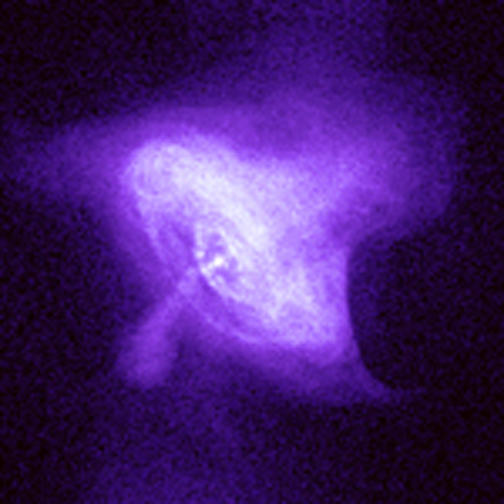
\includegraphics[width=0.5\columnwidth]{0052_xray_lg.jpg}
\end{center}
\caption{The central region of the Crab Nebula as seen by the Chandra
  X-ray Observatory. Credit: NASA/CXC/SAO)}
\label{fig:crab-xray}
\end{figure}

\begin{enumerate}
\item {\bf Hot cloud:} 

  X-ray photons are produced in a cloud of radius $R$ at the uniform
  rate $\Gamma$ (photons per unit volume per unit time) as in
  Fig.~\ref{fig:crab-xray}.  The cloud is a distance $d$ away.
  Assume that the cloud is optically thin.  A detector at Earth has an
  angular acceptance beam of half-angle $\Delta \theta$ and an
  effective area $\Delta A$.
\begin{enumerate}
\item If the cloud is fully resolved by the detector what is the
  observed intensity of the radiation as a function of position?
\item If the cloud is fully unresolved, what is the average intensity
  when the source is in the detector?
\end{enumerate}
\item {\bf Brightness Temperature:}
\index{temperature!brightness}

From the equation of radiative transfer derive an equation describing
how the brightness temperature changes as radiation passes through a
thermally emitting gas.  You may neglect scattering and assume that
the emission is in the Rayleigh-Jeans limit.  Solve this equation to
give the brightness temperature as a function of optical depth,
assuming that the gas has a constant temperature. 

\item {\bf Neutrino Blackbody:} 
\index{radiation!blackbody!neutrino}

Only one or no neutrinos can occupy a single state.  Calculate the
spectrum of the neutrino field in thermal equilibrium (neglect the
mass of the neutrino).  Neutrinos like photons have two polarization
states.  What is the ratio of the Stefan-Boltzmann constant for
neutrinos to that of photons?

\item {\bf Blackbody radiation:}
\begin{enumerate}
\item Show that if stimulated emission is neglected, leaving only two
  Einstein coefficients, an appropriate relation between the
  coefficients will be consistent with thermal equilibrium between an
  atom and a radiation field with a Wien spectrum, {\em i.e.} $B_\nu
  \propto \nu^3 \exp[-h\nu/(kT)]$.
\item Derive the relationships between the Einstein coefficients of an
  atom in equilibrium with a neutrino field.  
\end{enumerate}
\item {\bf Surface Emission from the Crab Pulsar:}  The neutron star
  that powers the Crab Pulsar can be assumed to have a mass of
  $1.4\mathrm{M}_\odot$ and a radius of 10~km with constant internal
  density and an effective temperature of $10^6$~K.  The frequency of
  the Crab Pulsar is 30~Hz and its period increases by 38 ns each
  day.  Compare the power from the surface emission to the power
  lost as the neutron star spins down.  The total power of the Crab
  Nebulae is about 75,000 times that of the Sun.  What is the likely
  source of this power?
\item {\bf Power-law Atmosphere:}  Assume the following
\begin{itemize}
\item The Rosseland mean
  opacity is related to the density and temperature of the gas through
  a power-law relationship,
$$
\kappa_R = \kappa_0 \rho^{\alpha} T^{\beta};
$$
\item The pressure of the gas is given by the ideal gas law;
\item The gas is in hydrostatic equilibrium so $p=g\Sigma$ where
$g$ is the surface gravity; and
\item The gas is in radiative equilibrium with the radiation field so 
the flux is constant with respect to $z$ or $\Sigma$.
\end{itemize}
Calculate the temperature of the gas as a function of $\Sigma$.
Assuming that the Crab pulsar has a surface or effective temperature
of $10^6$~K, what is the temperature at a density of
$10^7$~g/cm$^{-3}$ in the interior of the neutron star?  You may
assume $\alpha=2$, $g=10^{14}$ cm/s$^2$ and
$$
\kappa_R = 3.68 \times 10^{22} g_{ff}(1 - Z)(1 + X) \rho T^{-7/2} {\rm cm^2 g^{-1}}.
$$
where $\rho$ is given in g/cm$^{-3}$ and $T$ is given in Kelvin.

\item {\bf Goggles:}
\index{goggles}
Calculate from thermodynamic principles how much objects are magnified
or demagnified while viewed through goggles underwater.

\item {\bf Intensity and index of refraction: }
How does the intensity of light travelling along a ray change when the
light enters a material with a different index of refraction?
\begin{enumerate}
\item Solve this problem using geometry.
\item Solve this problem using thermodynamic principles alone.
N.B. The wavenumber of a photon of a given frequency is proportional
to the index of refraction.
\end{enumerate}
\end{enumerate}

 	
%%% Local Variables:
%%% TeX-master: "book"
%%% End:
\def\epbold{\mbox{\boldmath$\epsilon$}}
\chapter{Basic Theory of Radiation Fields}
\label{cha:basic-theory-radi}

\section{Maxwell's Equations}
\label{sec:maxwells-equations}
\index{electrodynamics!Maxwell's equations}
Most of this material is probably familar, so this will only present a
quick review.  The goals are to understand how charges move under the
influence of electromagnetic fields, how when the charges accelerate,
they emit electromagnetic radiation and how this radiation transports energy.
The electric and magnetic field may be
defined operationally by observing the motion of a particle of charge
$q$ travelling through the field.  The force on the particle is given
by the Lorentz force equation,
\begin{equation}
{\bf F} = q \left ( {\bf E} + \frac{\bf v}{c} \times {\bf B} \right ).
\label{eq:124}
\end{equation}
The fields perform work on the particle at a rate
\begin{equation}
{\bf v}\cdot {\bf F} = q {\bf v} \cdot {\bf E}.
\label{eq:125}
\end{equation}
One can imagine an ensemble of charged particles of charge density
$\rho$ and define the current to be ${\bf J}=\rho {\bf v}$.  In this
case we find that power delivered on the charges per unit volume is
simply
\begin{equation}
P = {\bf J} \cdot {\bf E}.
\label{eq:126}
\end{equation}
Note that the magnetic field ${\bf B}$ does not perform work on the
particle.   It changes the direction of the particle's motion but not
its speed.

The equations that describe the dynamics of the fields are Maxwell's
equations,
\begin{eqnarray}
{\bf \nabla} \cdot {\bf D} = 4\pi \rho & {\bf \nabla} \cdot {\bf B} =
0 \nonumber \\
{\bf \nabla} \times {\bf H} = \frac{4\pi}{c} {\bf J} +\frac{1}{c} 
\pp{\bf D}{t}
& {\bf \nabla} \times {\bf E} = -\frac{1}{c} \pp{\bf B}{t} 
\label{eq:127}
\end{eqnarray}
in Gaussian units.   The fields ${\bf D}$ and ${\bf H}$ are related to
${\bf E}$ and ${\bf B}$ through the constitutive relations
\begin{equation}
{\bf D} = \epsilon {\bf E}, {\bf B} = \mu {\bf H}, 
\label{eq:128}
\end{equation}
where $\epsilon$ and $\mu$ are in general matrices that depend on the
fields applied, but in most situations they are constant scalars and
for a vacuum they are simply one.

The equations were discovered by various people.  Proceeding left to
right then top to bottom we have Gauss's law, a law without a name,
Ampere's law and Faraday's law.  It might be more appropriate to call 
the penultimate, Maxwell's equation, because Ampere's law as it was
originally formulated was
\begin{equation}
{\bf \nabla} \times {\bf H} = \frac{4\pi}{c} {\bf J} 
\label{eq:129}
\end{equation}
Maxwell added the term proportional to the rate of change of the
electric field.  If one takes the divergence of the complete Ampere's
law one obtains,
\begin{equation}
{\bf \nabla} \cdot \left ( {\bf \nabla} \times {\bf H} \right ) = 
\frac{4\pi}{c} {\bf \nabla} \cdot {\bf J}  +
\frac{1}{c} {\bf \nabla} \cdot \pp{\bf D}{t}
\label{eq:130}
\end{equation}
The left-hand side vanishes because the divergence of the curl
vanishes, on the right hand side one obtains,
\begin{equation}
0 = \frac{4\pi}{c} {\bf \nabla} \cdot {\bf J}  +
\frac{4\pi}{c} \pp{\rho}{t}
\label{eq:131}
\end{equation}
where we have used the first of Maxwell's equations to simply the
result and find that the Maxwell's addition makes the full set of
equations consistent with charge conservation.

Let's calculate the work that the field will do on a bunch of charges
per unit volume,
\begin{equation}
{\bf J} \cdot {\bf E} = \frac{1}{4\pi} \left [ c \left ({\bf \nabla}
  \times {\bf H} \right ) \cdot {\bf E} - {\bf E} \cdot 
\pp{\bf D}{t} \right ]
\label{eq:132}
\end{equation}
We have the following vector identity (the triple product)
\begin{equation}
{\bf E} \cdot  \left ({\bf \nabla}
  \times {\bf H} \right ) = 
{\bf H} \cdot  \left ({\bf \nabla}
  \times {\bf E} \right ) - 
{\bf \nabla}  \cdot  \left ({\bf E}
  \times {\bf H} \right ) 
\label{eq:133}
\end{equation}
Substituting in the earlier result and using Faraday's law yields,
\begin{equation}
{\bf J} \cdot {\bf E} = \frac{1}{4\pi} \left [ - {\bf H} \cdot
  \pp{\bf B}{t} 
- {\bf E} \cdot 
\pp{\bf D}{t} 
- c
{\bf \nabla}  \cdot  \left ({\bf E}
  \times {\bf H} \right ) 
 \right ]
\label{eq:134}
\end{equation}
Let's assume that $\epsilon$ and $\mu$ are constant and get
\begin{equation}
{\bf J} \cdot {\bf E} + \frac{1}{8\pi} 
\pp{}{t} 
\left [ {\bf H} \cdot {\bf B}
+  {\bf E} \cdot  {\bf D} \right ] + {\bf \nabla}  \cdot  \left ( \frac{c}{4\pi}
{\bf E}  \times {\bf H} \right ) = 0
\label{eq:135}
\end{equation}
This is Poynting's theorem.  We can identify the work performed on the
charges, the change in the field energy per unit volume and the flux
of field energy (${\bf S}$) as follows,
\begin{equation}
U_{ \hbox{\rm \scriptsize field}} = \frac{1}{8\pi} \left [ {\bf H} \cdot {\bf B}
+  {\bf E} \cdot  {\bf D} \right ] ~~\hbox{\rm and}~~ {\bf S} = \frac{c}{4\pi} {\bf E}
  \times {\bf H}
\label{eq:136}
\end{equation}
\index{electrodynamics!Poynting vector}

\subsection{Waves}
\label{sec:waves}
\index{electrodynamics!waves}
Let's look at Maxwell's equations in a vacuum,
\begin{eqnarray}
{\bf \nabla} \cdot {\bf E} = 0 & & {\bf \nabla} \cdot {\bf B} =
0 \nonumber \\
{\bf \nabla} \times {\bf E} = -\frac{1}{c} \pp{\bf B}{t} & &
{\bf \nabla} \times {\bf B} = +\frac{1}{c} 
\pp{\bf E}{t} 
\label{eq:137}
\end{eqnarray}
Let's take the curl of the third equation and combine it with the
fourth to get
\begin{equation}
{\bf \nabla} \times \left ({\bf \nabla} \times {\bf E} \right ) =
-\frac{1}{c^2} \pp{^2 {\bf E}}{t^2}
\label{eq:138}
\end{equation}
We have the identity that
\begin{equation}
{\bf \nabla} \times \left ({\bf \nabla} \times {\bf E} \right ) =
{\bf \nabla} \left ( {\bf \nabla} \cdot {\bf E} \right ) - {\bf
  \nabla}^2 {\bf E}.
\label{eq:139}
\end{equation}
The first term on the right-hand side vanishes so we get the final
wave equation,
\begin{equation}
 {\bf   \nabla}^2 {\bf E}
-\frac{1}{c^2} \pp{^2 {\bf E}}{t^2} = 0
\label{eq:140}
\end{equation}
and a similar equation for the magnetic field.

We write a general solution to the wave equation as a sum of
harmonically varying waves such as 
\begin{equation}
{\bf E}= \Re \left ({\bf \hat a}_1 E_0 e^{i({\bf k \cdot r}-\omega t)}
\right )
~~\hbox{\rm and}~~~
{\bf B}= \Re \left ( {\bf \hat a}_2 B_0 e^{i({\bf k \cdot r}-\omega
  t)} \right )
\label{eq:141}
\end{equation}
Application of Maxwell's equations to the above solutions shows 
\begin{equation}
\nabla \cdot {\bf E} = i {\bf k} \cdot {\bf E} =0 ~\rmmat{so}~
{\bf \hat a}_{1} \perp {\bf k}
\label{eq:142}
\end{equation}
\begin{equation}
\nabla \cdot {\bf B} = i {\bf k} \cdot {\bf B} = 0~\rmmat{so}~
{\bf \hat a}_{2} \perp {\bf k}
\label{eq:143}
\end{equation}
\begin{equation}
\nabla \times {\bf E} + \frac{1}{c} \pp{\bf B}{t} = 
i {\bf k} \times {\bf E} - i \frac{\omega}{c} {\bf B} = 0
~\rmmat{so}~{\bf \hat a}_{1} \perp {\bf \hat a}_{2}
\label{eq:144}
\end{equation}
\begin{equation}
\nabla \times {\bf B} - \frac{1}{c} \pp{\bf E}{t} = 
i {\bf k} \times {\bf B} + i \frac{\omega}{c} {\bf E} = 0
~\rmmat{so}~\omega=kc~\rmmat{and}~E_0=B_0.
\label{eq:145}
\end{equation}

We would like to calculate the time-averaged energy density and energy
flux assoicated with the wave.  In general $E_0$ and $B_0$ are complex
quantities.  First let's look at the Poynting vector
\begin{eqnarray}
\left < {\bf S} \right > &=& \frac{1}{P} \int_0^P
\frac{c}{4\pi} {\bf E \times B} d t \\
&=& \frac{c{\bf \hat k}}{4\pi P} \int_0^P \!\!\!\!\!\!
d t
 \left ( \Re E_0 \cos \omega t 
- \Im E_0 \sin \omega t \right ) \times \nonumber \\ & & ~~~ \left ( \Re B_0 \cos \omega t 
- \Im B_0 \sin \omega t \right )   \\
&=&  \frac{c{\bf \hat k}}{4\pi P} \int_0^P \!\!\!\!\!\!
d t
 \left ( \Re E_0 \Re B_0 \cos^2 \omega t + \Im E_0 \Im B_0 \sin^2
 \omega t \right ) \\
&=&  \frac{c{\bf \hat k}}{8\pi} 
 \left ( \Re E_0 \Re B_0 + \Im E_0 \Im B_0 \right ) =
\frac{c{\bf \hat k}}{8\pi} \Re E_0^* B_0 \\
&=& \frac{c{\bf \hat k}}{8\pi} |E_0|^2= \frac{c{\bf \hat k}}{8\pi} |B_0|^2
\label{eq:146}
\end{eqnarray}
The time-averaged energy density is
\begin{equation}
\left < U \right > = \frac{1}{16\pi} \Re \left ( E_0 E_0^* + B_0 B_0^*
\right ) = \frac{1}{8\pi} |E_0|^2 = \frac{1}{8\pi} |B_0|^2
\label{eq:147}
\end{equation}
Because the electric and magnetic field have the same behaviour we
only have to describe one of the fields to determine the properties of the
wave.  It is customary to focus on the electric field.

\subsection{The Spectrum}
\label{sec:spectrum}
\index{electrodynamics!spectrum} A general electromagnetic wave can be
expressed as a sum of the Fourier components described in the previous
section.  We have been characterizing the energy in the radiation
field with the quantity $I_\nu$ the intensity per unit frequency
interval.  It would be nice to find an relationship between the
electric field as a function of time and the intensity.

\index{Fourier transform}
The first step in obtaining the spectrum is to take a Fourier
transform of the electric field of the wave
\begin{equation}
{\hat E} (\omega) = \frac{1}{2\pi} \int_{-\infty}^{\infty} E(t)
e^{i\omega t} d t.
\label{eq:148}
\end{equation}
The inverse of the this is
\begin{equation}
E (t) =  \int_{-\infty}^{\infty} {\hat E}(\omega)
e^{-i\omega t} d \omega.
\label{eq:149}
\end{equation}
Because $E(t)$ is real find that ${\hat E}(-\omega)={\hat
  E}^*(\omega)$ so we don't have to keep track of the negative
frequencies.

To study the energy carried by the wave we look at the Poynting vector
\begin{equation}
\frac{d W}{d t d A} = \frac{c}{4\pi} E^2(t)
\ee 
The total energy per unit area in the wave is 
\begin{equation}
\frac{d W}{d A} = \frac{c}{4\pi} \int_{-\infty}^{\infty} E^2(t) dt
\label{eq:150}
\end{equation}
Parseval's theorem (see \S~\ref{sec:an-math-asid} for a proof) for Fourier transforms states that
\begin{equation}
\int_{-\infty}^{\infty} |E|^2(t) dt = 2\pi \int_{-\infty}^{\infty} 
|{\hat E}(\omega)|^2 d \omega.
\label{eq:151}
\end{equation}
Additionally, because ${\hat E}(-\omega)={\hat
  E}^*(\omega)$ we have
\begin{equation}
\int_{-\infty}^{\infty} E^2(t) dt = 4\pi \int_0^{\infty} 
|{\hat E}(\omega)|^2 d \omega.
\label{eq:152}
\end{equation}
and we can write
\begin{equation}
\frac{d W}{d A} = c \int_0^{\infty} 
|{\hat E}(\omega)|^2 d \omega.
\label{eq:153}
\end{equation}
And we obtain that 
\begin{equation}
\frac{d W}{d A d \omega } = c |{\hat E}(\omega)|^2
\label{eq:154}
\end{equation}
The intensity is related to the energy per unit time.   If the pulse
repeats on a time scale $T$ or the wave changes only on timescales $T$
much longer than $1/\omega$ we may define
\begin{equation}
\frac{d W}{d A d \omega d t} = \frac{c}{T} |{\hat E}(\omega)|^2
\label{eq:155}
\end{equation}
Table~\ref{tab:fourier} gives a few Fourier transforms of common
functions.  Although the last one seems rather arcane it has an important
property,
\begin{equation}
\int \frac{\sin \left [T    (\omega-\omega') \right ]}{\pi (\omega -
  \omega')} d\omega = 1
\label{eq:156}
\end{equation}
that lets us define the pair
\begin{eqnarray}
E(t) &=& e^{-i\omega' t} \\
{\hat E}(\omega) &=& \delta (\omega-\omega')
\label{eq:157}
\end{eqnarray}
where 
\begin{equation}
\int \delta(\omega-\omega') f(\omega) d\omega = f(\omega')
\label{eq:158}
\end{equation}

\begin{table}
\caption{Some Useful Fourier transforms}
\label{tab:fourier}
\begin{center}
\begin{tabular}{cc}
\hline \\
$E(t)$ &  ${\hat E}(\omega)$ \\  \\ \hline \\
\begin{minipage}[c]{0.3\columnwidth}
\begin{center}
\tikz \draw (0,0)--(0.5,0)--(0.5,0.5)--(1,0.5)--(1,0)--(1.5,0)
(0.75,0) node {$w$} (1.25,0.25) node {$h$}  (0.75,0.7) node {$t_0$};
\end{center}
\end{minipage}
& $\frac{h}{\pi \omega} \sin \frac{\omega w}{2} e^{i\omega t_0}$
 \\
\begin{minipage}[c]{0.3\columnwidth}
\begin{center}
\tikz \draw (0,0)--(0.5,0)--(0.75,0.5)--(1,0)--(1.5,0);
\end{center}
\end{minipage}
  & 
$\frac{2 h}{\pi w \omega^2} \left ( 1 - \cos \frac{\omega w}{2} \right ) e^{i\omega t_0}$
\\ \\
$\exp \left ( -\frac{\left(t-t_0\right)^2}{2\sigma^2} \right )$ & 
$e^{i\omega t_0} \exp
\left ( -\frac{\omega^2 \sigma^2}{2} \right )
\sqrt{\frac{\sigma^2}{2\pi}}$ \\ \\
$e^{-a|t|}$ &  $\frac{1}{2\pi} \frac{a}{a^2+\omega^2}$ \\ \\
$\exp \left ( - i \omega' t \right ) ~\hbox{\rm for}~ |t|<T$ &
$\frac{\sin \left [T    (\omega-\omega') \right ]}{\pi (\omega -
  \omega')}$ 
\\ \\
\hline
\end{tabular}
\end{center}
\end{table}

\section{Polarization}
\label{sec:polar-stok-param}
\index{electrodynamics!polarization}
\index{radiation!polarization}
For a general electromagnetic wave with wavenumber ${\bf k}$ we can
define a basis for the polarization of the wave:
$\epbold_1$ and $\epbold_2$ such that 
$\epbold_1 \times \epbold_2 ~\|~ {\bf k}$.   For example a wave can 
be linearly polarized with its electric field always pointing along 
$\epbold_1$ or along $\epbold_2$.   A
general solution is a linear combination of these two waves with
complex coefficients.  To be more specific we have
\begin{eqnarray*}
{\bf E}_1 &=& \epbold_1 E_1 e^{i{\bf k}\cdot {\bf x} - i \omega t} \\
{\bf E}_2 &=& \epbold_2 E_2 e^{i{\bf k}\cdot {\bf x} - i \omega t}\\
{\bf B}_j &=& \frac{{\bf k}\times {\bf E}_j}{k} \\
\label{sec:polar-stok-param-1}\end{eqnarray*}
and a general wave would be ${\bf E}={\bf E}_1 + {\bf E}_2$.  Because
the coefficients $E_1$ and $E_2$ are complex we can introduce a phase
difference between the two perpendicular components.  If this phase
difference is zero, then the wave is linearly polarized (left panel of
Fig.~\ref{fig:polar}) with the
polarization vector making an angle $\theta=\tan^{-1}(E_2/E_1)$ with
$\epbold_1$ and a magnitude of $E=\sqrt{E_1^2+E_2^2}$

\begin{figure}
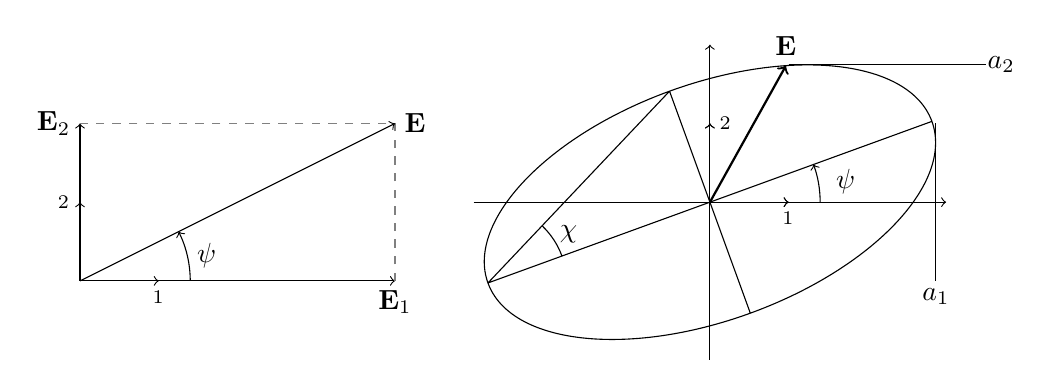
\begin{tikzpicture}
\draw [->] (0,0) -- (0,1) ;
\draw [->] (0,0) -- (0,2) ;
\draw [->] (0,0) -- (1,0) ;
\draw [->] (0,0) -- (4,0) ;
\draw [dashed,gray] (4,0) -- (4,2) -- (0,2) ;
\draw [->] (0,0) -- (4,2) ;
\draw [->] (1.4,0) arc (0:26.57:1.4) ;
\draw (1,0) node [below] {$\epbold_1$}  
(0,1) node [left]  {$\epbold_2$}
(4,0) node [below] {${\bf E}_1$}  
(0,2) node [left] {${\bf E}_2$}  
(4,2) node [right] {${\bf E}$} 
(13.28:1.4) node [right] {$\psi$} ;
\begin{scope}[shift={(8,1)}]
\draw (1,1.75)-- ++(2.5,0) ++(0.2,0) node {$a_2$}
(2.87,1)-- ++(0,-2) ++(0,-0.2) node {$a_1$};
\draw [rotate=20] (0,0) ellipse (3 and 1.5) (-3,0) -- (3,0) 
(0,-1.5) -- (0,1.5) 
(1.5,1.2990381057) node [above] {${\bf E}$} 
(-3,0) -- (0,1.5) (-2,0) arc (0:26.565834671:1) (-3,0)
++(18:1) node [right] {$\chi$};
\draw [->] (1.4,0) arc (0:20:1.4);
\draw [->] (0,0) -- (0,1) ;
\draw [->] (0,0) -- (1,0) ;
\draw [->] (0,0) -- (0,1) ;
\draw [->] (0,-2) -- (0,2) ;
\draw [->] (0,0) -- (1,0) ;
\draw [->] (-3,0) -- (3,0) ;
\draw [->,rotate=20,thick] (0,0) -- (1.5,1.2990381057);
\draw (1,0) node [below] {$\epbold_1$}  
(0,1) node [right] {$\epbold_2$}
(10:1.5) node [right] {$\psi$} ;
\end{scope}
\end{tikzpicture}
\caption{Electric field of linearly (left) and elliptically (right)
  polarized waves}
\label{fig:polar}
\end{figure}


If the phase difference is nonzero, one in genral has an elliptically
polarized wave as shown in the right panel of Fig.~\ref{fig:polar}.
The orientation of the ellipse is characterized by the
orientation, tile or azimuth angle $\psi$ which is the angle between
the semimajor axis of the ellipse and $\epbold_1$.  The shape of the
ellipse is measured by the ellipticity, $\epsilon$, the ratio of the
lengths of the major to minor axes.  We can also define an ellipticity
angle $\chi=\cot^{-1} \epsilon$.  The sign of $\chi$ is positive for
a right-hand circularly polarized wave --- in this case the electric field would
proceed anti-clockwise in Fig.~\ref{fig:polar}.

One could have defined an alternative representation based on the
circular polarizations
\begin{equation}
\epbold_\pm = \frac{1}{\sqrt{2}} \left ( \epbold_1 \pm i \epbold_2
\right ).
\label{eq:162}
\end{equation}
Because $\epbold_\pm$ is now complex one has to be a bit careful
about its orthogonality properties.  Specifically,
\begin{equation}
\epbold_\pm^* \cdot \epbold_\mp = 0,
\epbold_\pm^* \cdot {\bf k} = 0,
\epbold_\pm^* \cdot \epbold_\pm = 1.
\label{eq:163}\end{equation}
Often it is convenient to use this circular polarization basis rather
than the linear polarization basis above (for example, waves
travelling through plasma).

Most astronomical detectors blueward of the microwave measure not the
electric field directly but rather the energy delivered by the wave.
It is possible to recover this polarization information through
intensity measurements.

Generally one inserts a filter which collapses the incoming wave onto
one of the polarization states and one measures the resulting
intensity.  For example,  the intensity measured through a polarizing
filter aligned along the $1-$direction is $|\epbold_1 \cdot {\bf
  E}|^2$.   Let be more explicit and take two examples,
\begin{eqnarray*}
E_1 &=& a_1 e^{i\delta_1},~~~  E_2 = a_2 e^{i\delta_2} \\
E_+ &=& a_+ e^{i\delta_+},~~~  E_- = a_- e^{i\delta_-}.
\end{eqnarray*}
The first wave is given in the linear basis and the second is given in
the circular basis.  One typically makes a series of intensity
measurements through filters and quarter wave plates with different
orientations and combines the resulting intensities to form the
Stokes parameters, $I,Q,U$ and $V$ or $s_0,s_1,s_2$ and $s_3$.
The first parameter measures the total intensity of the wave, the sum
of the intensities of the two linearly polarized measurements.

\subsection{Stokes Parameters}
\index{radiation!Stokes parameters}
In the linear polarization basis we have
\begin{eqnarray*}
I &=& s_0 = |\epbold_1 \cdot {\bf E}|^2 + |\epbold_2 \cdot {\bf
  E}|^2 = a_1^2 + a_2^2 \\
Q &=& s_1 = |\epbold_1 \cdot {\bf E}|^2 - |\epbold_2 \cdot {\bf
  E}|^2 = a_1^2 - a_2^2 \\
U &=& s_2 = 2 \Re \left [ (\epbold_1 \cdot {\bf E})^* (\epbold_2 \cdot {\bf
  E}) \right ] = 2 a_1 a_2 \cos \left (\delta_2 - \delta_1 \right ) \\
V &=& s_3 = 2 \Im \left [ (\epbold_1 \cdot {\bf E})^* (\epbold_2 \cdot {\bf
  E}) \right ] = 2 a_1 a_2 \sin \left (\delta_2 - \delta_1 \right ) \\
\end{eqnarray*}
and for the circular basis we have 
\begin{eqnarray*}
I &=& s_0 = |\epbold_+ \cdot {\bf E}|^2 + |\epbold_- \cdot {\bf
  E}|^2 = a_+^2 + a_-^2 \\
Q &=& s_1 = 2 \Re \left [ (\epbold_+ \cdot {\bf E})^* (\epbold_- \cdot {\bf
  E}) \right ] = 2 a_+ a_- \cos \left (\delta_- - \delta_+ \right ) \\
U &=& s_2 = 2 \Im \left [ (\epbold_+ \cdot {\bf E})^* (\epbold_- \cdot {\bf
  E}) \right ] = 2 a_+ a_- \sin \left (\delta_- - \delta_+ \right ) \\
V &=& s_3 = |\epbold_+ \cdot {\bf E}|^2 - |\epbold_- \cdot {\bf
  E}|^2 = a_+^2 - a_-^2 \\
\end{eqnarray*}
The fractional polarization is given by
\begin{equation}
\Pi = \frac{\sqrt{Q^2+U^2+V^2}}{I}.
\label{eq:164}
\end{equation}
and the fractional linear polarization
\begin{equation}
\Pi_l = \frac{\sqrt{Q^2+U^2}}{I}.
\label{eq:165}
\end{equation}
The four Stokes parameters satisfy the following relationship for a
truly monochromatic wave
\begin{equation}
s_0^2 = s_1^2 + s_2^2 + s_3^2.
\label{eq:166}
\end{equation}

\subsection{Poincar\'e Sphere}
\index{radiation!Poincar\'e sphere}

This result shows that the Stoke's parameters live on a sphere of
radius $r\leq s_0$ where the extent of polarization $\Pi=r/s_0$.
This sphere of polarization is known as the Poincar\'e sphere
(Fig.~\ref{fig:poincare}) and the
location of the polarization on the sphere is related to the
orientation of the polarization ellipse in Fig.~\ref{fig:polar}.  In
particular we have
\begin{eqnarray*}
s_1 &=& Q = \Pi I \cos2\psi \cos 2\chi \\
s_2 &=& U = \Pi I \sin2\psi \cos 2\chi \\
s_3 &=& V = \Pi I \sin 2\chi
\end{eqnarray*}
which relates Stoke's parameters to the orientation and shape of the
polarization ellipse.  The two angles defined in Fig.~\ref{fig:polar}
related to the latitude ($2\chi$) and longitude ($2\psi$) of the
polarization vector $(s_1,s_2,s_3)$ on the Poincar\'e sphere.

\begin{figure}
\begin{center}
\input figures/poincare
\end{center}
\caption{The Poincar\'e sphere}
\label{fig:poincare}
\end{figure}

An interesting and useful relationship is that the Stokes
parameters are additive for waves whose phases are not correlated.
Let's take two waves of frequencies $\omega_a$ and $\omega_b$ and
calculate the value of the first Stokes parameter as an example.  We have
\begin{eqnarray}
\label{eq:167}
I &=& s_0 = |\epbold_1 \cdot {\bf E}|^2 + |\epbold_2 \cdot {\bf
  E}|^2 \\
&=& \frac{1}{\Delta t} \int_0^{\Delta t}   \biggr [
\left |
\epbold_1 \cdot {\bf E}_a e^{-i\omega_a t} + \epbold_1 \cdot {\bf E}_b 
e^{-i\omega_b t} \right |^2 + \nonumber \\
& & ~~~~~~
\left |
\epbold_2 \cdot {\bf E}_a e^{-i\omega_a t} + \epbold_2 \cdot {\bf E}_b 
e^{-i\omega_b t} \right |^2 \biggr ] d t \\
&=& 
\frac{1}{\Delta t} \int_0^{\Delta t}   \biggr \{
\left | \epbold_1 \cdot {\bf E}_a \right |^2  +
\left |  \epbold_1 \cdot {\bf E}_b \right |^2 +
\left | \epbold_1 \cdot {\bf E}_a \right |^2  +
\left |  \epbold_1 \cdot {\bf E}_b \right |^2 + \nonumber \\
& & ~~~ 
2 \left [ \left ( \epbold_1 \cdot {\bf E}_a \right ) 
\left ( \epbold_1 \cdot {\bf E}_b \right ) +
\left ( \epbold_2 \cdot {\bf E}_a \right ) 
\left ( \epbold_2 \cdot {\bf E}_b \right )  \right ]
\cos \left [ \left (\omega_a-\omega_b\right ) t \right ] \biggr \}
\label{eq:168} \\
&=& s_{0,a} + s_{0,b} + 
\left \{ 
\begin{array}{cl}
\mathcal{O} \left [ \sqrt{s_{0,a}
      s_{0,b}}
 \left ( \Delta \omega \Delta t \right)^{-1} \right ]
& \Delta\omega \Delta t \gg 1 \\
\mathcal{O} \left [ \sqrt{s_{0,a}
      s_{0,b}} \left ( \Delta \omega \Delta t \right )  \right ]
& \Delta\omega \Delta t \ll 1 
\end{array} \right .
\end{eqnarray}
where $\Delta \omega = \omega_a-\omega_b$. For example, if we look at
a star over a wide range of frequencies (the definition of wide is 
$\Delta \omega \Delta t \gg\ 1$), the phase of waves at one end of the 
frequency range will not correlate with waves at the other end.  

When we measure the Stokes parameters in practice we measure for example
\begin{equation}
s_2 = 2 \left < a_1 a_2 \cos \left (\delta_2 - \delta_1 \right )
\right >.
\label{eq:169}
\end{equation}
Although $\cos^2 x + \sin^2 x = 1$, $0\leq \left <\cos x\right>^2  +
\left <\sin x\right>^2 \leq 1$, so for a quasimonochromatic wave we
have
\begin{equation}
s_0^2 \geq s_1^2 + s_2^2 + s_3^2.
\label{eq:170}
\end{equation}
Because the Stokes parameters are additive and measure the energy
content of the wave, they are a natural basis to calculate the
radiative transfer of polarized radiation.

\section{Electromagnetic Potentials}
\label{sec:electr-potent}
\index{electrodynamics!potentials}
Looking at the structure of Maxwell's equations, we can see that we can 
express the magnetic field as the curl of another field, the vector potential,
\begin{equation}
\nabla \cdot {\bf B} = \nabla \cdot (\nabla \times {\bf A}) = 0 
\label{eq:171}
\end{equation}
where the second equality is an identity if ${\bf B} = \nabla \times
{\bf A}$. 

Let's substitute this into the other homogenous Maxwell
equation,
\begin{eqnarray}
\nabla \times {\bf E} + \frac{1}{c} \pp{}{t} \nabla \times {\bf A} &=& 0 \\*
\nabla \times \left ( {\bf E} + \frac{1}{c} \pp{\bf A}{t} \right ) &=& 0
\end {eqnarray}
If
\begin{equation}
-\nabla\phi =  {\bf E} + \frac{1}{c} \pp{\bf A}{t} 
\label{eq:172}
\end{equation}
then the second homogeneous Maxwell equation is satisfied as well.

Let's recap
\begin{eqnarray}
{\bf B} &=& \nabla \times {\bf A} \\
{\bf E} &=& -\nabla \phi - \frac{1}{c} \pp{\bf A}{t} \\
\label{eq:173}
\end{eqnarray}
The expression of the fields in terms of the vector and scalar
potential guarantees that two out of four of Maxwell's equations are
satisfied.  Let's substitute our results into the remaining Maxwell's
equations,
\begin{eqnarray}
\nabla \cdot {\bf E} &=& 4\pi\rho \\
\nabla \cdot \left ( -\nabla \phi - \frac{1}{c} \pp{\bf A}{t} \right ) &=& 4\pi \rho \\
\nabla^2 \phi +  \frac{1}{c} \pp{}{t} \nabla \cdot {\bf A}&=& -4\pi \rho
\label{eq:174}
\end{eqnarray}
and the second inhomogeneous equation gives
\begin{eqnarray}
\nabla \times {\bf B} - \frac{1}{c} \pp{\bf E}{t} &=& \frac{4\pi}{c} {\bf J} \\
\nabla \times \left ( \nabla \times {\bf A} \right ) + \frac{1}{c} \pp{}{t} \left ( \nabla \phi + \frac{1}{c} \pp{\bf A}{t} \right )&=& \frac{4\pi}{c} {\bf J} \\
\nabla \left ( \nabla \cdot {\bf A} \right ) - \nabla^2 {\bf A} + \frac{1}{c} \pp{}{t} \left ( \nabla \phi + \frac{1}{c} \pp{\bf A}{t} \right )&=& \frac{4\pi}{c} {\bf J} 
\label{eq:175}
\end{eqnarray}
Now let's rearrange the last equation a bit more,
\begin{eqnarray}
-\nabla \left ( \nabla \cdot {\bf A} \right ) +  \nabla^2 {\bf A} - \frac{1}{c} \pp{}{t} \left ( \nabla \phi \right ) - \frac{1}{c^2} \pp{^2 {\bf A}}{t^2} &=& -\frac{4\pi}{c} {\bf J}  \\
  \nabla^2 {\bf A}
- \frac{1}{c^2} \pp{^2 {\bf A}}{t^2}
-\nabla \left ( \nabla \cdot {\bf A}  + \frac{1}{c} \pp{\phi}{t}  \right ) &=& -\frac{4\pi}{c} {\bf J} 
\label{eq:176}
\end{eqnarray}
Let's look at the last of the charge density equations equations some more,
\begin{eqnarray}
\nabla^2 \phi +  \frac{1}{c} \pp{}{t} \nabla \cdot {\bf A}&=& -4\pi \rho \\*
\nabla^2 \phi - \frac{1}{c^2} \pp{^2 \phi}{t^2} +  \frac{1}{c} \pp{}{t} \left ( \nabla \cdot {\bf A}
+\frac{1}{c} \pp{\phi}{t} \right )&=& -4\pi \rho 
\label{eq:177}
\end{eqnarray}
Although it looks like that the equation is a bit more complicated than before, it now 
has the precise form of the equation with the current.   

Wouldn't life be simpler if the quantity in the parenthesis in both equations vanished?
Guess what?   We can choose for it to vanish by making a good choice
of gauge.  Only the electric and magnetic fields are measurable so we
can make any change to the potentials ${\bf A}$ and $\phi$ that we
want as long at ${\bf E}$ and ${\bf B}$ remain unchanged.  Because
${\bf B} = \nabla \times {\bf A}$ we can add the gradient of any
function $\psi$ to ${\bf A}$ without changing ${\bf B}$ (the curl of a
gradient of a function is zero).

However, if we add a gradient of function to ${\bf A}$ the value of
${\bf E}$ is affected,
\begin{equation}
{\bf E} \rightarrow {\bf E} - \frac{1}{c} \pp{}{t}
\nabla \psi.
\label{eq:178}
\end{equation}
To fix this we also have to change the scalar potential $\phi$ at the
same time by subtracting  $1/c ( \partial \psi/\partial t )$ from
$\phi$.   Therefore, we find that the equations of electromagnetism
remain unchanged if one replaces
\begin{equation}
{\bf A} \rightarrow {\bf A} + \nabla \psi ~~\hbox{\rm and}~~ \phi \rightarrow \phi -
\frac{1}{c} \pp{\psi}{t}
\label{eq:179}
\end{equation}
This is the gauge transformation and it means that we in general have
the freedom to set a particular scalar constraint on the potentials.

\subsection{Lorenz Gauge}
\index{electrodynamics!Lorenz gauge}

In particular we would like to set
\begin{equation}
 \nabla \cdot {\bf A}
+\frac{1}{c} \pp{\phi}{t} = 0
\label{eq:180}
\end{equation}
This is equivalent to finding a function $\psi$ that satisfies
\begin{equation}
\nabla^2 \psi - \frac{1}{c^2} \pp{^2 \psi}{t^2} +\nabla \cdot {\bf A}
+\frac{1}{c} \pp{\phi}{t} = 0
\label{eq:181}
\end{equation}
and adding it to ${\bf A}$ to get ${\bf A}'$.  It turns out that this
is possible so we are free to use the following equations for the
potentials,
\begin{equation}
\nabla^2 \phi - \frac{1}{c^2} \pp{^2 \phi}{t^2} =
-4\pi \rho,~~\hbox{\rm and}~~
  \nabla^2 {\bf A}
- \frac{1}{c^2} \pp{^2 {\bf A}}{t^2} =
-\frac{4\pi}{c} {\bf J}.
\label{eq:182}
\end{equation}
This is the Lorenz gauge (which happens to be {\em Lorentz}
invariant).

\subsection{Green's Function}

Both of the equations have the same form.  Let's look at the equation
for the electric field
\begin{equation}
\nabla^2 \phi - \frac{1}{c^2} \pp{^2 \phi}{t^2} = -4\pi \rho 
\label{eq:804}
\end{equation}
and write $\phi$ and $\rho$ in terms of their Fourier transforms in
time, e.g.
\begin{equation}
\rho({\bf r},t) = \int_{-\infty}^\infty \hat \rho ({\bf r}, \omega)
e^{-i\omega t} d t
\label{eq:805}\end{equation}
so the equation for the potential now looks like
\begin{equation}
\nabla^2 \hat \phi({\bf r},\omega) + \frac{\omega^2}{c^2} \hat \phi({\bf
  r},\omega) = -4\pi \hat \rho(\bf r,\omega) .
\label{eq:806}\end{equation}
Now let's look for a particular solution $G({\bf r},\omega)$ for $\hat
\phi$ where $\hat \rho$ vanishes everywhere but the origin
\begin{equation}
\nabla^2 \hat G({\bf r},\omega) + \frac{\omega^2}{c^2} \hat G({\bf
  r},\omega) = -4\pi \delta(\bf r).
\label{eq:807}\end{equation}
The function $G({\bf r},\omega)$ is the Green's function of the
equation (Eq.~\ref{eq:806}).   It is a useful concept because
Maxwell's equations are linear, so the principle of superposition
applies.  The electromagnetic fields for two charges is simply the sum
of the fields of each charge on its own.

Because the right-hand side only depends on the magnitude
of ${\bf r}$, the Green's function must be spherically symmetric, so
\begin{equation}
\frac{1}{r} \pp{^2}{r^2} \left [ r \hat G(r,\omega) \right ] + \frac{\omega^2}{c^2} \hat G(r,\omega) = -4\pi \delta(r)
\label{eq:808}
\end{equation}
which is nearly the equation for the potential for a point change.

We can start with the solution $1/r$ and add an exponential term to
handle the second term in the equation; let's substitute the following
ansatz
\begin{equation}
\hat G(r,\omega) = \frac{e^{ikr}}{r}
\label{eq:809}
\end{equation}
which yields
\begin{equation}
-k^2 \frac{e^{ikr}}{r} + \frac{\omega^2}{c^2} \frac{e^{ikr}}{r} =
-4\pi \delta(r)
\label{eq:812}
\end{equation}
which trivially solves the equation everywhere but the origin if 
$k=\pm \omega/c$.  Because Eq.~\ref{eq:808} is a second-order
differential equation we get two solutions,
\begin{equation}
{\hat G}^{\pm}(r,\omega) = \frac{e^{i \pm r \omega/c}}{r}
\label{eq:810}
\end{equation}
and the complete solution is a linear combination of the two.  Now
because we know the solution for source at a point we can write the
solution for a distribution of charge
\begin{equation}
\hat \phi^{\pm}({\bf r}, \omega) = \int d^3 r' \frac{\exp \left (
    \pm i\omega/c |{\bf r}-{\bf r}'|/c \right )  }{|{\bf r}-{\bf r}'|} \hat \rho({\bf r}',\omega) 
\label{eq:811}
\end{equation}
and write out the potential as a function of time
\begin{equation}
\phi^{\pm}({\bf r}, t) = \int d^3 r' d \omega \frac{\exp \left [
    -i\omega \left ( t \mp |{\bf r}-{\bf r}'|/c \right ) \right
  ]}{|{\bf r}-{\bf r}'|} \hat \rho({\bf r}',\omega) .
\label{eq:813}
\end{equation}
We can perform the integral over time because it is the same as
Eq.~(\ref{eq:805}) but with $t$ replaced by $t \mp |{\bf r}-{\bf
  r}'|/c$, so we have
\begin{equation}
\phi^{\pm}({\bf r}, t) = \int d^3 r' \rho \left ({\bf r}, t \mp
\frac{|{\bf r}-{\bf r}'|}{c} \right ) \frac{1}{|{\bf r}-{\bf r}'|}.
\label{eq:824}
\end{equation}

The solution for the vector potential is similar.  We have two choices
(or a linear combination).  The potential here can depend on the
locations of charges along the past and the future light cones.
Although the latter choice appears to violate causality, it all
really depends on what questions that you would like to ask.  For
example, if you wanted to know given the distribution of fields here
and now, what would be the distribution of charges to absorbed the
radiation in the future, then the {\bf advanced} potential (with the plus
sign after the time coordinate).   Here we are generally interested in
the radiation that a configuration of charges emit, so we shall use
the {\bf retarded} potentials,
\begin{eqnarray}
{\bf A}({\bf r},t) &=& \frac{1}{c} \int d^3 r' \frac{{\bf J}\left ({\bf
  r}',t-\frac{|{\bf r}-{\bf r}'|}{c} \right )}{|{\bf r} -
{\bf  r}'|} \\
\phi({\bf r},t) &=& \int d^3 r' \frac{\rho\left ({\bf
  r}',t-\frac{|{\bf r}-{\bf r}'|}{c} \right )}{|{\bf r} -
{\bf  r}'|} .
\label{eq:183}
\end{eqnarray}

\section{Further Reading}

To learn more about faint x-ray structure in the Crab nebula, consult
\begin{itemize}
\item Seward, F.~D., Tucker, W.~H. \& Fesen, R.~A.\ 2006, ``Faint X-Ray Structure in the Crab Pulsar Wind Nebula,'' {\em ApJ}, 652, 1277 
\end{itemize}
and 
\begin{itemize}
\item Heyl, J.~S. \& Shaviv, N.~J.\ 2000, ``Polarization evolution in
  strong magnetic fields,'' {\em MNRAS}, 311, 555 
\end{itemize}
use the Poincar\'e sphere extensively to study how the polarization of
emission from the surface of the Crab pulsar changes as it travels
through the star's magnetic field.

The general development of Maxwell's equations and the polarization of
radiation are examined in Chapter~6 and \S\S~7.1-7.2 of
\begin{itemize}
\item Jackson, J. D., {\em Classical Electrodynamics}.
\end{itemize}

\section{Problems}

\begin{enumerate}
\item{\bf  Coulomb's Law}

Derive Coulomb's law from Maxwell's Equations.

\item {\bf Ohm's Law and Absoption:} 

In certain cases the process of aborption of radiation can be treated
by means of the macroscopic Maxwell equations. For example, suppose we
have aconducting medium so that the current density ${\bf j}$ is related to
the electric field ${\bf E}$ by Ohm's law: ${\bf J} = \sigma {\bf E}$ where
$\sigma$ is the conductivity (cgs unit = $\mathrm{sec}^{-1}$). Investigate the
propagation of electromagnetic waves in such a medium and show that:
\begin{enumerate}
\item The wave vector ${\bf k}$ is complex
$$
{\bf k}^2 = \frac{\omega^2 m^2}{c^2}
$$
where $m$ is the complex index of refraction with
$$
m^2 = \mu \epsilon \left ( 1 + \frac{4 \pi i \sigma}{\omega \epsilon}
\right )
$$
\item The waves are attenuated as they propagate, corresponding to an
absorption coefficient.
$$
\alpha = \frac{2\omega}{c} \Im (m)
$$

\end{enumerate}

\begin{figure}
\begin{center}
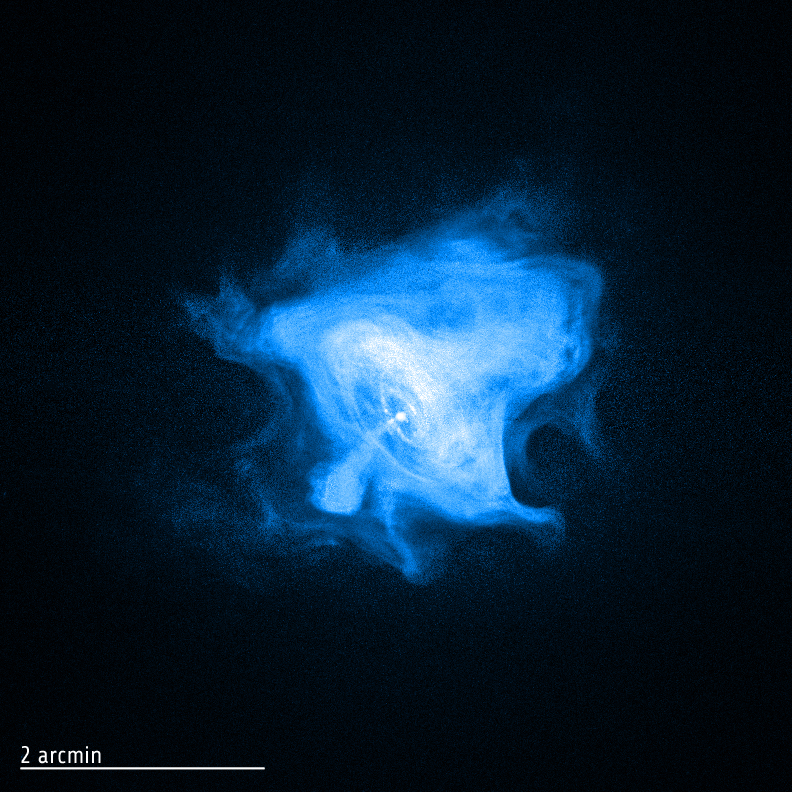
\includegraphics[width=0.5\columnwidth]{crab_scale.jpg}
\end{center}
\caption{A Chandra image of the outskirts of the Crab pulsar wind
  nebula. Credit: NASA/CXC/SAO/F.Seward et al }
\label{fig:crab-edge}
\end{figure}

\item {\bf The Edge of the Crab}

  Fig.~\ref{fig:crab-edge} shows the x-ray emission of the Crab pulsar
  wind nebula at a distance of 2~kpc.  The x-ray emitting gas is
  contained by magnetic fields causing the x-ray emission regions to
  end sharply.  We can relate the frequency of the emission to the energy
  of the electrons and the strength of the magnetic field by
\begin{equation}
\omega = \left ( \frac{E}{m_e c^2}
\right )^2 \frac{e B}{m_e c} 
\end{equation}
and assume that the electrons are relativistic so their inertial mass
is $E/c^2$.  Use the sharpness of the emission
regions to determine the energy of the electrons and the strength of
the magnetic field.

\item {\bf Momentum and Angular Momentum: } 

This problem is meant to deduce the momentum and angular momentum
properties of radiation and does not recesarily represent any real
physical system of interest. Consider a charge $Q$ in a viscous medium
where the viscous force is proportional to velocity: 
$$
F_\rmscr{visc} = -\beta v
$$
Suppose a circular polarized wave passes through the medium. The
equation of motion of the charge is 
$$
m \dd{v}{t} = F_\rmscr{visc} + F_\rmscr{Lorentz}
$$
We assume that the terms on the right dominate the inertial term on the
left, so that approximately 
$$
0 = F_\rmscr{visc} + F_\rmscr{Lorentz}
$$
Let the frequency of the wave be $\omega$ and the strength of the
electric field be E.
\begin{enumerate}
\item
Show that to lowest order (neglecting the magnetic force) the crage
moves on a circle in a plane normal to the direction of propagation of
the wave with speed $QE/\beta$ and with radius $QE/(\beta \omega)$.
\item
Show that the power transmitted to the fliud by the wave is $Q^2 E^2/\beta$
\item
By considering the small magnetic force acting on the particle show
that the momentum per unit time (force) given to the fluid by the wave
is in the direction of propagation and has the magnitude 
$Q^2 E^2/(\beta c)$
\item
Show that the angular momentum per unit time (torque) given to the
fliud by the wave is in the direction of propagation and has magnitude
$\pm Q^2 E^2/(\beta \omega0$ where the + is for left and - is for
right circular polarization.
\item
Show that the absorption cross section of the charge is
$4\pi Q^2/(\beta c)$.
\item
 If we regard the radiation to be composed of circular polarized
 photons of energy $E_\gamma= h \nu$, show that these results imply that the
 photon has momemtum $p=h/\lambda=E_\gamma/c$ and has angular momemtum 
$J=\pm \hbar$ along the direction of propagation.
\item
 Repeat this problem for a linearly polarized wave
\end{enumerate}

\item {\bf Maxwell's equations before Maxwell: }

Show that Maxwell's equations before Maxwell, that is, without the
"displacement current" term, $c^{-1} \pp{D}{t}$, unacceptably constrained the
sources of the field and also did not permit the existence of waves.

\item {\bf Coulomb gauge} 
Derive the equations describing the dynamics of the electric and
vector potentials in the Coulomb gauge
$$
\nabla \cdot {\bf A} = 0
$$
Look at the equation for the electric potential. What is the solution
to the electric potential given the charge density $\rho$? Why is this
called the Coulomb gauge?

How does the expression for the scalar potential in the Coulomb gauge
differ from that in the Lorenz gauge? What is strange about it? Is it
physical?

Now look at the equation for the vector potential. Show that the LHS
can be arranged to be the same as in the Lorenz gauge but the RHS is
not just the current but the current plus something else.

Show that the RHS can be expressed as 
$$
\frac{4\pi}{c} \left ( {\bf J} - {\bf J}_\rmscr{long} \right ) 
$$
where
$$
{\bf J}_\rmscr{long} = -\frac{1}{4\pi} \nabla \int \frac{\nabla' \cdot
{\bf J}}{|{\bf x}-{\bf x}'|} d^3 x
$$
\end{enumerate}

%%% Local Variables:
%%% TeX-master: "book"
%%% End:

\chapter{Radiation from Moving Charges}
\label{cha:radi-from-moving}
We will start to look at how radiation gets produced, scattered
and absorbed at a microscopic level to derive quantities like $j_\nu$,
$\alpha_\nu$ and $\sigma_\nu$.

\section{Retarded Potentials}
\label{sec:retarded-potentials}
\index{electrodynamics!retarded potentials}
We saw in the last section that in the Lorenz gauge the equations for
the vector and scalar potential are
\begin{equation}
\nabla^2 \phi - \frac{1}{c^2} \frac{\partial^2 \phi}{\partial t^2} =
-4\pi \rho,~~\hbox{\rm and}~~
  \nabla^2 {\bf A}
- \frac{1}{c^2} \frac{\partial^2 {\bf A}}{\partial t^2} =
-\frac{4\pi}{c} {\bf J}.
\label{eq:184}
\end{equation}
which have the following solution
\begin{eqnarray}
{\bf A}({\bf r},t) &=& \frac{1}{c} \int d^3 r' \frac{{\bf J}\left ({\bf
  r}',t-\frac{|{\bf r}-{\bf r}'|}{c} \right )}{|{\bf r} -
{\bf  r}'|} \\
\phi({\bf r},t) &=& \int d^3 r' \frac{\rho\left ({\bf
  r}',t-\frac{|{\bf r}-{\bf r}'|}{c} \right )}{|{\bf r} -
{\bf  r}'|} .
\label{eq:185}
\end{eqnarray}
An equivalent way of writing $\phi({\bf r},t)$ is
\begin{equation}
\phi({\bf r},t) = \int d^3 r' \int dt' \frac{\rho \left ({\bf
  r}',t'\right )}{|{\bf r} -
{\bf  r}'|} \delta ( t' - t + |{\bf r}-{\bf r}'|/c ) 
\label{eq:186}
\end{equation}
and similarly for ${\bf A}$

Let's think about a single charge with charge $q$ and position 
${\bf  r}_0(t)$.   It can be characterized by
\begin{equation}
\rho({\bf r},t) = q \delta({\bf r} -{\bf r}_0(t))~~\hbox{\rm
  and}~~{\bf j}(r, t) = q {\bf u} \delta({\bf r} - {\bf r}_0(t))
\label{eq:187}
\end{equation}
Let's substitute this expression for $\rho$,
\begin{eqnarray}
\phi({\bf r},t) &=& 
\int d^3 r' \int dt' \frac{q \delta({\bf r}'-{\bf r}_0(t'))}{|{\bf r} -
{\bf  r}'|} \delta ( t' - t + |{\bf r}-{\bf r}'|/c )  \\
 &=& 
q \int dt' \frac{1}{|{\bf r} -
{\bf  r}_0(t')|} \delta ( t' - t + |{\bf r}-{\bf r}_0(t')|/c )  
\label{eq:188}
\end{eqnarray}
It is easy to perform integrals over a $\delta$-function if the
integral is over the argument of the $\delta$-function, so we 
would like to perform the following change of variables
\begin{equation}
t'' = t' - t +  \frac{|{\bf r}-{\bf r}_0(t')|}{c}
\label{eq:189}
\end{equation}
yielding the Li\'enard-Wiechert potentials
\index{electrodynamics!Li\'enard-Wiechert potentials}
\begin{eqnarray}
\phi({\bf r},t) &=& 
q \int dt'' \frac{1}{|{\bf r} -
{\bf  r}_0(t')|} \delta ( t'' ) \frac{\partial t'}{\partial t''} \\
&=& \frac{q}{R(t_\rmscr{ret}) \kappa (t_\rmscr{ret})}\\
{\bf A} &=& \frac{q{\bf u}(t_\rmscr{ret})}{cR(t_\rmscr{ret}) \kappa (t_\rmscr{ret})}
\label{eq:190}
\end{eqnarray}
where
\begin{eqnarray}
R(t) &=& |{\bf r} - {\bf r}_0(t)| \\
t_\rmscr{ret} &=& t - \frac{R(t_\rmscr{ret})}{c} \\
\kappa(t) &=&  \frac{\partial t''}{\partial t'}.
\label{eq:191}
\end{eqnarray}
Let's look at the partial derivative now,
\begin{eqnarray}
\kappa(t) &=&  \frac{\partial t''}{\partial t'} = 1 + \frac{1}{c}
\frac{\partial R(t)}{\partial t}
\label{eq:192}
\end{eqnarray}
and looking at $R(t)$
\begin{equation}
R(t)^2 = {\bf R}(t) \cdot {\bf R}(t) 
\label{eq:193}
\end{equation}
so
\begin{equation}
2 R(t) {\dot R}(t) = -2 {\bf R}(t) \cdot {\bf u}(t) ~~\rmmat{NB:} ~~{\bf R} = {\bf r}-{\bf r}_0(t)
\label{eq:194}
\end{equation}
so
\begin{equation}
\kappa(t) = 1 - \frac{1}{c} \frac{{\bf R}(t) \cdot {\bf u}(t)}{R(t)} = 1 - \frac{1}{c} {\bf n}(t) \cdot {\bf u}(t).
\label{eq:195}
\end{equation}

\subsection{The Fields}
\label{sec:fields}
\index{electrodynamics!moving charges}
We can use the potentials to determine the electric and magnetic
fields produced by the moving particle.  Let us define
\begin{equation}
\betabold \equiv \frac{\bf u}{c},~\rmmat{so}~ \kappa = 1 - {\bf n} \cdot \betabold
\label{eq:196}
\end{equation}
which yield the fields (see \S~14.1 of Jackson)
\begin{eqnarray}
{\bf E}(r,t) &=& \kern-2mm q \left [ \frac{({\bf n} - \betabold)(1-\beta^2)}{\kappa^3 R^2} \right ]_\mathrm{ret}\!+\!\frac{q}{c} \left [ \frac{\bf n}{\kappa^3 R} \times \left [ 
({\bf n} - \betabold ) \times \dot{\betabold} \right ]\right ]_\mathrm{ret} \\
{\bf B}(r,t) &=& \kern-2mm\left [ {\bf n} \times {\bf E}(r,t) \right ]_\mathrm{ret}.
\label{eq:197}
\end{eqnarray}
It is important to remember that all of the properties of the particle
are evaluated at the retarded time.

A few things to notice are that if the particle is not accelerating
the electric field points to the current not the retarded position of
the particle.  This allows us to graphically depict the field for a
particle that is stopped suddenly.

The fields have two parts.  The first part is proportional to $1/R^2$
and it is simply a generalization of the field for a stationary
charge.  The second terms are proportional to $1/R$.  They are
\begin{eqnarray}
{\bf E}_\rmscr{rad}(r,t) &=& + \frac{q}{c} \left [ \frac{\bf n}{\kappa^3 R} \times \left [ 
({\bf n} - \betabold ) \times \dot{\betabold} \right ]\right ] \\
{\bf B}_\rmscr{rad}(r,t) &=& \left [ {\bf n} \times {\bf E}_\rmscr{rad}(r,t) \right ].
\label{eq:198}
\end{eqnarray}

\comment{
A fun thing to calculate is the Poynting vector of the fields for zero
acceleration
\begin{eqnarray}
{\bf S} &=&  \frac{c}{4\pi} {\bf E} \times {\bf B}\\
        &=&  \frac{c}{4\pi} \left ( {\bf E} \times ({\bf n} \times
        {\bf E} \right ) \\
	&=& \frac{c}{4\pi} \left [ {\bf n} \left ({\bf E} \cdot {\bf
        E}\right ) - {\bf E} \left ({\bf E}\cdot {\bf n} \right )
        \right ].
\label{eq:199}
\end{eqnarray}
Let's work through the first term,
\begin{equation}
{\bf n} \left ( {\bf E} \cdot {\bf E} \right ) = q^2 {\bf n} \frac{(1 - 2 {\bf n}\cdot
  \betabold + \beta^2)(1-\beta^2)^2}{\kappa^6 R^4}
\label{eq:200}
\end{equation}
Let's work on the second term now
\begin{eqnarray}
{\bf E} \left ( {\bf E} \cdot {\bf n} \right ) &=& q {\bf E} \left [ \frac{(1-\beta^2)}{\kappa^2 R^2}
  \right ] \\
&=&  q^2 \left [ \frac{({\bf n} - \betabold)(1-\beta^2)}{\kappa^3 R^2}
  \right ] 
 \left [ \frac{(1-\beta^2)}{\kappa^2 R^2}
  \right ] \\
&=& q^2  \frac{({\bf n} - \betabold)(1-\beta^2)^2}{\kappa^5 R^4}
\label{eq:201}
\end{eqnarray}
\begin{eqnarray}
{\bf S} &=&  \frac{c}{4\pi} 
\frac{q^2 (1-\beta^2)^2}{\kappa^6 R^4}
\left [ {\bf n} \left ( 1 - 2 {\bf n}\cdot \betabold + \beta^2 \right
  ) 
- \left ( {\bf n} - \betabold \right) \kappa \right ]\\
&=& \frac{c}{4\pi} 
\frac{q^2 (1-\beta^2)^2}{\kappa^6 R^4}
\left [ {\bf n} \left (  \betabold \cdot ( \betabold - {\bf n} )\right
  )
 + \betabold \kappa \right ]
\label{eq:202}
\end{eqnarray}
}

We can calculate the Poynting vector of the radiation fields
\begin{equation}
{\bf S} = {\bf n} \frac{q^2}{4\pi c \kappa^6 R^2} \left | {\bf n} \times
\left \{ \left ( {\bf n} - \betabold \right ) \times {\dot{\betabold}}
\right \} \right |^2
\label{eq:203}
\end{equation}

\subsection{Distribution in Frequency and Angle}
\label{sec:distr-freq-angle}

To examine the spectrum of the radiation let us define examine the
Fourier transform of the electric field.  We know (Eq.~\ref{eq:154})
\begin{equation}
\frac{dW}{dAd\omega} = c |\hat E(\omega)|^2
\label{eq:814}
\end{equation}
where
\begin{equation}
{\hat E} (\omega) = \frac{1}{2\pi} \int_{-\infty}^{\infty} E(t) e^{i\omega t} d t.
\label{eq:816}
\end{equation}
in our case we are interested in the energy emitted per solid angle so
\begin{equation}
\frac{dW}{d\Omega d\omega} = R^2 \frac{dW}{dA d\omega}= c |R \hat E(\omega)|^2
\end{equation}
and
\begin{equation}
R {\hat E} (\omega) = \frac{q}{2\pi c} \int_{-\infty}^{\infty}
\left [ \frac{\bf n}{\kappa^3} \times \left [ 
({\bf n} - \betabold ) \times \dot{\betabold} \right ]\right ]_\mathrm{ret}
e^{i\omega t} d t.
\label{eq:817}
\end{equation}
The intergrand is evaluated at the retarded time, $t'+R(t')/c=t$, so
we can change the variable of integration from $t$ to $t'$ to yield
\begin{equation}
R {\hat E} (\omega) = \frac{q}{2\pi c} \int_{-\infty}^{\infty}
\left [ \frac{\bf n}{\kappa^2} \times \left [ 
({\bf n} - \betabold ) \times \dot{\betabold} \right ]\right ]
e^{i\omega (t'+R(t')/c)} d t'.
\label{eq:818}
\end{equation}
If we assume that the observer is far away from where the acceleration
occurs, the unit vector ${\bf n}$ can be taken to be constant and
$R(t') \approx R_0 - {\bf n} \cdot {\bf r}(t')$, yielding
\begin{equation}
R {\hat E} (\omega) = \frac{q}{2\pi c} \int_{-\infty}^{\infty}
\left [ \frac{\bf n}{\kappa^2} \times \left [ 
({\bf n} - \betabold ) \times \dot{\betabold} \right ]\right ]
e^{i\omega (t'-{\bf n}\cdot {\bf r}(t')/c)} d t'.
\label{eq:819}
\end{equation} 
As we did earlier (\S~\ref{sec:spectrum}), the total energy radiated
per unit angle is
\begin{equation}
\frac{d W}{d\Omega d\omega} =
\frac{q^2}{4\pi^2 c} \left | \int_{-\infty}^{\infty}
\frac{{\bf n} \times \left [  ({\bf n} - \betabold ) \times
    \dot{\betabold} \right ]}{\left ( 1-\betabold\cdot {\bf n} \right )^2}
e^{i\omega (t'-{\bf n}\cdot {\bf r}(t')/c)} d t' \right |.
\label{eq:825}
\end{equation}
The expression can be simplied further by noticing that
\begin{equation}
\frac{{\bf n} \times \left [  ({\bf n} - \betabold ) \times
    \dot{\betabold} \right ]}{\left ( 1-\betabold\cdot {\bf n} \right
  )^2}
= \frac{d}{d t'} \left [ \frac{{\bf n} \times ({\bf n} \times
    \betabold ) }{1-\betabold\cdot {\bf n}} \right ].
\label{eq:820}
\end{equation}
and integrating Eq.~\ref{eq:819} by parts to yield
\begin{equation}
\frac{d W}{d\omega d\Omega} = \frac{q^2 \omega^2}{4\pi^2 c^3} 
\left | \int_{-\infty}^\infty {\bf n} \times ({\bf n} \times \betabold) e^{i
  \omega \left ( t'-{\bf n} \cdot {\bf r}_0 (t') / c \right )} dt'
\right |^2.
\label{eq:204}
\end{equation}

\subsection{Non-relativistic particles}
\label{sec:non-relat-part}
\index{electrodynamics!moving charges!non-relativistic}

Let's assume that $|\betabold| \ll 1$ and focus on a particular
frequency $\nu$ so that ${\dot u} \sim u \nu$.  We can compare the
``acceleration'' fields to the ``velocity'' field
\begin{eqnarray}
{\bf E}_\rmscr{acc} &=& \frac{q}{c^2 R} \left [ {\bf n} \times
    \left \{ {\bf n} \times \dot{\bf u} \right \} \right ] 
    \\
{\bf E}_\rmscr{vel} &=& \frac{q {\bf n}}{R^2}
\label{eq:205}
\end{eqnarray}
so
\begin{equation}
\frac{E_\rmscr{acc}}{E_\rmscr{vel}} \sim \frac{R \dot{u}}{c^2} \sim
\frac{R u \nu}{c^2} = \frac{u}{c} \frac{R}{\lambda}
\label{eq:206}
\end{equation}
so for points in the ``near zone'', $R\leq \lambda$, the velocity
field is stronger than the acceleration field by a factor $\geq c/u$; but
for points sufficiently far into the ``far zone'', $R\gg\ \lambda
(c/u)$, the acceleration field dominates.

Let's derive {\bf Larmor's formula} for the radiated energy.  Let use
the angle $\Theta$ to denote the angle between the vectors ${\bf n}$
and $\dot{{\bf u}}$, so we have
\begin{equation}
|{\bf E}_\rmscr{acc}| = |{\bf B}_\rmscr{acc}| = \frac{q \dot{u}}{Rc^2}
\sin \Theta
\label{eq:207}
\end{equation}
Using the formula for the Poynting vector we have
\begin{equation}
{\bf S} = {\bf n} \frac{c}{4\pi} E_\rmscr{acc}^2 = \frac{c}{4\pi}
\frac{q^2 \dot{u}^2}{R^2 c^3} \sin^2 \Theta
\label{eq:208}
\end{equation}
The power radiated per unit solid angle is simply $\left ( {\bf S}\cdot {\bf
  n}\right) R^2$ or
\begin{equation}
\frac{dW}{dt d\Omega} = \frac{q^2 \dot{u}^2}{4\pi c^3} \sin^2 \Theta
\label{eq:209}
\end{equation}
Let's integrate over all angles to get the power
\begin{eqnarray}
P &=& \frac{d W}{d t} = \frac{q^2 \dot{u}^2}{4\pi c^3} \int
\sin^2\Theta d\Omega = \frac{q^2 \dot{u}^2}{2 c^3}\int_{-1}^1 \left (1
- \mu^2 \right ) d \mu  \\
&=& \frac{2 q^2 \dot{u}^2}{3c^3}
\label{eq:210}
\end{eqnarray}

\subsection{How about relativistic particles?}
\label{sec:how-about-relat}
\index{electrodynamics!moving charges!relativistic}

Let's look at the Poynting vector again.
\begin{equation}
{\bf S} = {\bf n} \frac{q^2}{4\pi c \kappa^6 R^2} \left | {\bf n} \times
\left \{ \left ( {\bf n} - \betabold \right ) \times {\dot{\betabold}}
\right \} \right |^2
\label{eq:211}
\end{equation}
where ${\bf S}\cdot {\bf n}$ is the energy per unit area per unit time
detected at an observation poiint at time $t$ of radiation emitted by
the charge at time $t'=1-R(t')/c$.  Let's calculate the energy radiated away from $t'=T_1$ to $t'=T_2$ we would have
\begin{equation}
E = \int_{t=T_1+[R(T_1)/c]}^{t=T_2+[R(T_2)/c]}\left [{\bf S}\cdot {\bf n} \right ] d t
= \int_{T_1}^{T_2}\left [{\bf S}\cdot {\bf n} \right ] \frac{dt}{dt'} dt'
\label{eq:212}
\end{equation}
so we have
\begin{equation}
\frac{dP(t')}{d\Omega} = R^2 \left ({\bf S}\cdot {\bf n} \right )  \frac{dt}{dt'} = R^2  \left ({\bf S}\cdot {\bf n} \right ) \left ( 1 - \betabold \cdot n\right ) 
\label{eq:213}
\end{equation}
When we include the Poynting vector expression we have
\begin{equation}
\frac{dP(t')}{d\Omega} = \frac{q^2}{4\pi c} \frac{ \left | {\bf n} \times
\left \{ \left ( {\bf n} - \betabold \right ) \times {\dot{\betabold}}
\right \} \right |^2}{\left ( 1 - {\bf n} \cdot \betabold \right )^5}
\label{eq:214}
\end{equation}
Let's start by assuming the $\betabold$ is parallel to ${\dot{\betabold}}$, so  
$\betabold \times {\dot{\betabold}}=0$.  We get
\begin{equation}
\frac{dP(t')}{d\Omega} = \frac{q^2 {\dot u}^2}{4\pi c^3} 
\frac{ \sin^2 \Theta }{\left ( 1 - \beta \cos\Theta  \right )^5}
\label{eq:215}
\end{equation}
Let's integrate the power over all angles,
\begin{equation}
P = 2\pi \frac{q^2 {\dot u}^2}{4\pi c^2} \int_{-1}^1 
\frac{1-\mu^2}{\left ( 1 - \beta \mu \right )^5} d\mu = \frac{2}{3} \frac{q^2 {\dot u}^2}{c^2} \gamma^6
\label{eq:216}
\end{equation}
where
\begin{equation}
\gamma = \frac{1}{\sqrt{1-\beta^2}}=\frac{1}{\sqrt{(1+\beta)(1-\beta)}}
\label{eq:217}
\end{equation}
Let's take a second look at the angular distribution of power for small angles and 
$\beta \approx 1$.
\begin{eqnarray}
\frac{dP(t')}{d\Omega} &\approx&  \frac{q^2 {\dot u}^2}{4\pi c^3} 
\frac{ \theta^2 }{\left [ 1 - (1 - \gamma^{-2}/2 ) (1 - \theta^2/2 )
  \right ]^5} \\
&\approx &
 \frac{q^2 {\dot u}^2}{4\pi c^3} 
\frac{ \theta^2 }{\left [ \gamma^{-2}/2 + \theta^2/2   \right ]^5} \\
&\approx& \frac{8}{\pi}
 \frac{q^2 {\dot u}^2}{c^3} \gamma^8
\frac{ (\gamma \theta)^2 }{\left [ 1 + (\gamma \theta)^2   \right ]^5} 
\label{eq:218}
\end{eqnarray}
{
\begin{figure}
\centering
%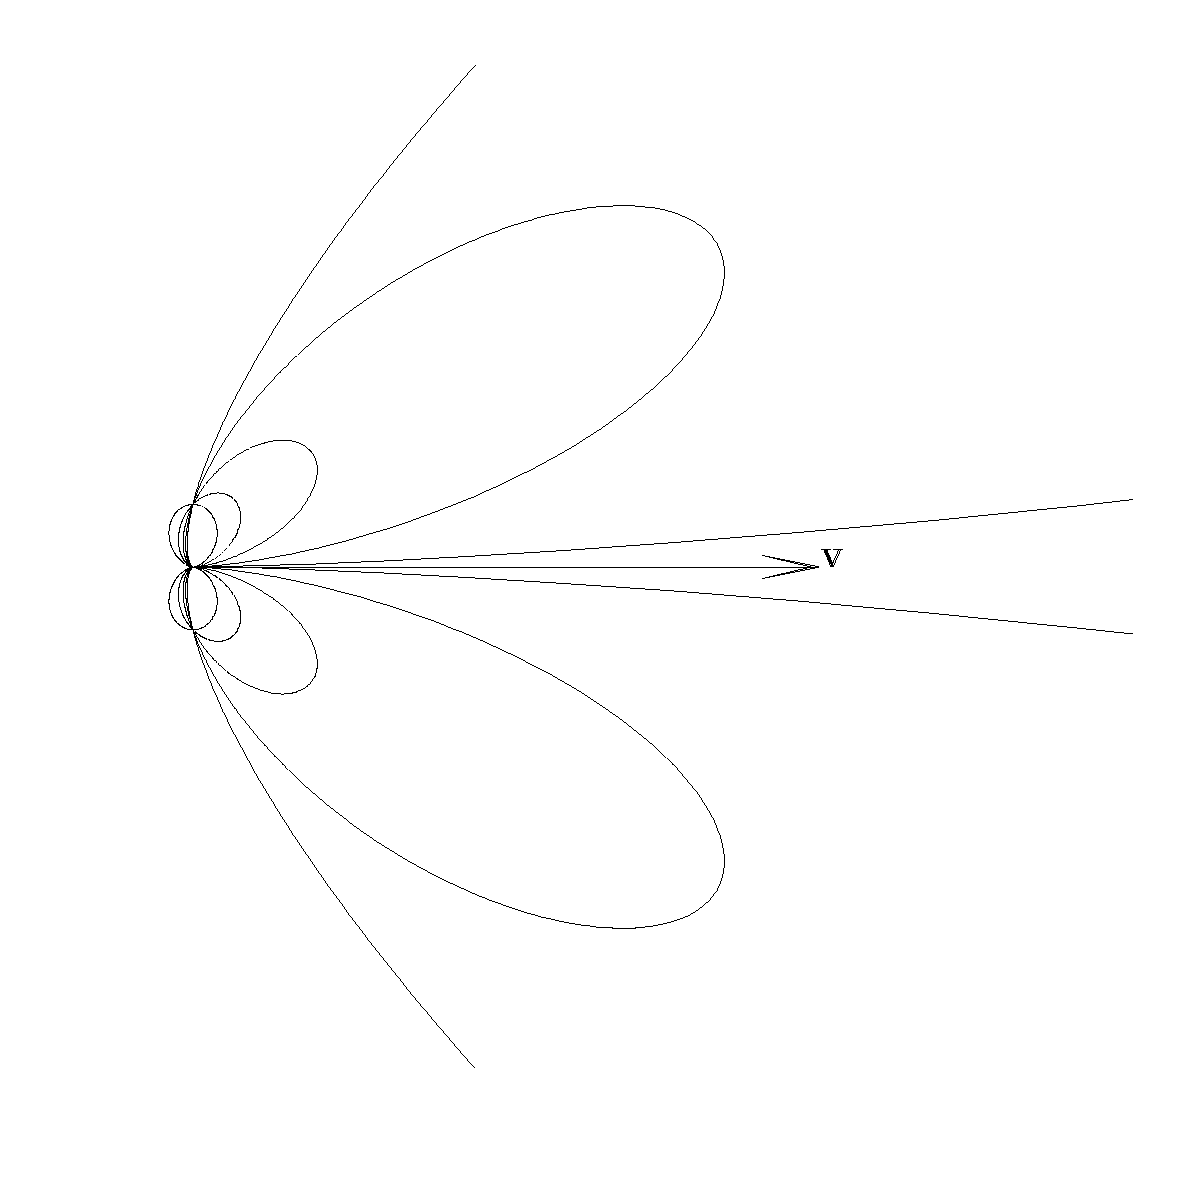
\includegraphics[width=0.45\textwidth]{sp}
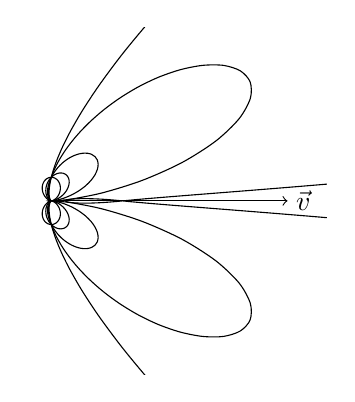
\begin{tikzpicture}
\clip (-0.3,-2.2) rectangle (3.5,2.2);
\foreach \b in {0, 0.2, 0.4, 0.6, 0.8} 
\draw plot [domain=0:360,smooth,samples=100] ( {-0.3*cos(\x)*sin(\x)^2/(1+\b*cos(\x))^5} ,
{0.3*sin(\x)^3/(1+\b*cos(\x))^5});
\draw [->] (0,0)--(3,0);
\draw (3.2,0) node {$\vec v$};
\end{tikzpicture}
% \includegraphics[width=0.45\textwidth]{rp2} 
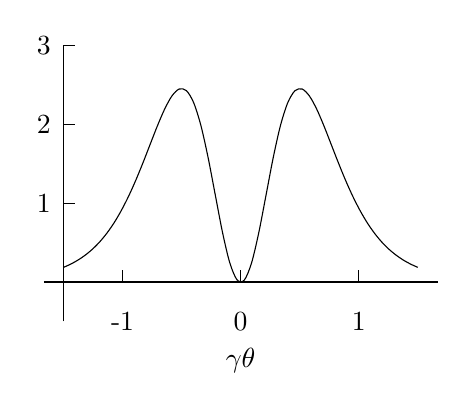
\begin{tikzpicture}
\draw plot [domain=-1.5:1.5,samples=50,smooth] ( {1.5*\x} , { \x*\x /
  (1+\x*\x)^5 *30 });
\draw  (-2.5,0)--(2.5,0) ;
\draw  (-2.25,-0.5)--(-2.25,3) ;
\draw (0,-1) node {$\gamma\theta$} ;
\foreach \x in { -1, 0, 1 }
  \draw (1.5*\x,-0.5) node {\x} (1.5*\x,0)--(1.5*\x,0.15);
\foreach \y in { 1, 2, 3 }  
  \draw (-2.5,\y) node {\y} (-2.25,\y) -- (-2.1,\y) ;
\end{tikzpicture}
\caption{Radiated power as a function of angle and $\gamma \theta$ for
  longitudinal motion. The left-hand panel shows from inside out
  $\beta=0,0.2,0.4,0.6,0.8$.}
\end{figure}
}

Let's repeat the calculation for circular motion, in which $\betabold
\perp {\dot{\betabold}}$.  To be definitive we have to specify two
angles for our observer ${\bf n}$.  Let's take the velocity to be
along the $z$-axis and the accelation along the $z$ axis, so $\Theta$
is the angle between ${\bf n}$ and the velocity and $\phi$ is the
angle between the projection of the vector ${\bf n}$ into the $x-y$-plane 
and the acceleration ({\em i.e.} these are just ordinary spherical coordinates). We obtain in general,
\begin{equation}
\frac{dP(t')}{d\Omega} = \frac{q^2 {\dot u}^2}{4\pi c^3} 
\frac{ 1 }{\left ( 1 - \beta \cos\Theta  \right )^3}
\left [ 1 - 
\frac{ \sin^2 \Theta \cos^2\phi }{\gamma^2 \left ( 1 - \beta \cos\Theta  \right )^2} \right ]
\label{eq:219}
\end{equation}
If we integrate this over all angles we get
\begin{equation}
P(t') = \frac{2}{3} \frac{q^2 {\dot u}^2}{c^3} \gamma^4
\label{eq:220}
\end{equation}
At first glance, the power from longitudinal motion seems much larger that the circular 
motion, but it is important to compare the power emitted for the same applied force ($d{\bf p}/dt$).

For circular motions the applied force is $\gamma m {\dot u}$, yielding
\begin{equation}
P_\rmscr{circ}(t') = \frac{2}{3} \frac{q^2}{m^2 c^3} \gamma^2 \left ( \frac{d {\bf p}}{d t}\right )^2
\label{eq:221}
\end{equation}
For longitudinal acceleration, the applied force is given by $m \gamma^3 {\dot u}$
\begin{equation}
P_\rmscr{long}(t') = \frac{2}{3} \frac{q^2}{m^2 c^3} \left ( \frac{d {\bf p}}{d t}\right )^2
\label{eq:222}
\end{equation}
For a given applied force, the radiation due to the component
perpendicular to the motion is much larger than the parallel
component.  If the particles are ultrarelativistic it is appropriate
to neglect the parallel contribution completely.

\subsection{Radiation from Systems of Particles}
\label{sec:radi-from-syst}

Let's focus back on the radiation from a non-relativistic particle,
specifically a bunch of such particles.  The electric field is linear
so the total electric field of the ensemble is the sum of the
particle's individual contributions,
\begin{equation}
{\bf E}_\rmscr{tot} = \sum_i
 \frac{q_i}{c^2 R_i} \left [ {\bf n}_i \times
    \left \{ {\bf n}_i \times \dot{\bf u}_i \right \} \right ] 
\label{eq:223}
\end{equation}
This sum could get really cumbersome, especially if you have $\sim
10^{40}$ particles.  You have to calculate the retarded position and
keep track of the velocity of each one.   There is an easier way.

Let's assume that the particles are confined to a region of size $l$
and we are really far from that region, $R_i \gg\ l$ so $R_i \approx
R$ where $R$ is the distance to the centre of the region and ${\bf n}_i
\approx {\bf n}$, a vector pointing to the centre of the region.

For the above expression for the electric field to be valid, $R/c$
must be greater than any timescale ($\tau$ for the particles to change
position ({\em i.e.} we are in the ``far'' zone).  Let's also assume that
$c\tau \gg\ l$ which means that we can neglect the difference in
retarded time between particles at one end of the region and the
other.  Let's make these changes
\begin{equation}
{\bf E}_\rmscr{tot} = \frac{1}{c^2 R} 
 \left [ {\bf n} \times
    \left \{ {\bf n} \times  \sum_i q_i \dot{\bf u}_i \right \} \right ] 
\label{eq:224}
\end{equation}
Let's define the dipole moment of the ensemble
\begin{equation}
{\bf d} = \sum_i q_i {\bf r}_{0,i}
\label{eq:225}
\end{equation}
which yields
\begin{equation}
{\bf E}_\rmscr{tot} = \frac{1}{c^2 R} 
 \left [ {\bf n} \times
    \left \{ {\bf n} \times  \ddot {\bf d} \right \} \right ] 
\label{eq:226}
\end{equation}
We also get
\begin{equation}
\frac{d P}{d \Omega} = \frac{\ddot{\bf d}^2}{4\pi c^3} \sin^2 \Theta
~~\rmmat{and}~~ P=\frac{2 \ddot{\bf d}^2}{3c^3}
\label{eq:227}
\end{equation}
Let's examine the spectrum of dipole radiation.  To make things
easier, let us assume that the dipole lies in a single direction and
varies in magnitude (imagine a negative charge moving up and down a
wire).  In this case the electric field is parallel to ${\bf d}$ and
we have
\begin{equation}
E(t) = \ddot{d} (t) \frac{\sin \Theta}{c^2 R}
\label{eq:228}
\end{equation}
Let's define 
\begin{equation}
d(t) = \int_{-\infty}^\infty e^{-i\omega t} {\hat d}(\omega) d \omega
\label{eq:229}
\end{equation}
so we have
\begin{equation}
\ddot{d}(t) = -\int_{-\infty}^\infty \omega^2 e^{-i\omega t} {\hat d}(\omega) d \omega
\label{eq:230}
\end{equation}
so
\begin{equation}
{\hat E}(\omega) = - \frac{1}{c^2 R_0} \omega^2 {\hat d}(\omega) \sin \Theta
\label{eq:231}
\end{equation}
and the power per unit solid angle and frequency is
\begin{equation}
\frac{dW}{d \omega d\Omega} = \frac{1}{c^3} \omega^4 |{\hat
  d}(\omega)|^2 \sin^2 \Theta ~\rmmat{and}~ \frac{dW}{d\omega} =
\frac{8\pi \omega^2}{3c^3} |{\hat d}(\omega)|^2
\label{eq:232}
\end{equation}

\subsection{A Physical Aside: Multipole Radiation}
\label{sec:phys-asid-mult}
\index{electrodynamics!multipole radiation}

It is possible to calculate the radiation field to higher order in
$L/(c\tau)$.  This is necessary if the dipole moment vanishes, for
example.   We can expand the exponential to yield
\begin{equation}
A_\omega ({\bf r}) = \frac{e^{ikr}}{cr} \sum_{n=0}^\infty \frac{1}{n!}
\int {\bf j}_\omega ({\bf r}') \left ( -ik{\bf n}\cdot {\bf r}' \right
)^n d^3 r'
\label{eq:233}
\end{equation}
where $k\equiv\omega/c$  $n=0$ gives the dipole radiation, $n=1$ gives
the quadrupole radiation and so on.

\section{Cherenkov Radiation}
\label{sec:cherenkov-radiation}
\index{electrodynamics!Cherenkov radiation}
\index{Cherenkov radiation}
\index{Cerenkov radiation}
\index{electrodynamics!moving charges!Cherenkov radiation}

\newcommand{\waves}[1]{
  \fill (0,0) circle (0.02);
  \draw [->,thick] (-1.6*#1,0)--(0,0) ;
  \draw [dashed] (-1.6*#1,0)--(-1.6*#1,-2.4) 
                 (0,0) -- (0,-2)
                 (-1.6*#1+1.6,0) -- (-1.6*#1+1.6,-2.4);
  \draw [<-] (-1.6*#1,-2.3) -- (-1.6*#1+0.6,-2.3) ;
  \draw [->] (-1.6*#1+1.0,-2.3) -- (-1.6*#1+1.6,-2.3) ;
  \draw (-1.6*#1+0.8,-2.3) node {$ct$};
  \draw [<-] (-1.6*#1,-1.9) -- (-0.8*#1-0.2,-1.9) ;
  \draw [->] (-0.8*#1+0.2,-1.9) -- (0,-1.9) ;
  \draw (-0.8*#1,-1.9) node {$vt$};
   \foreach \t in {0.2,0.4,...,1.6} \draw (-\t*#1,0) circle (\t);
}
\begin{figure}
\begin{center}
\begin{tikzpicture}
\waves{0.5}
\draw (-0.8,-2.8) node {$v<c/\sqrt{\epsilon}$};
\begin{scope}[shift={(6,0)}]
\waves{1.5}
\draw (-1.118033989*2,2) -- (0,0) -- (-1.118033989*2,-2);
\draw (-2,-2.8) node {$v>c/\sqrt{\epsilon}$};
\draw [->] (-2.4,0) -- ++(48.191106385:2);
\draw  (-1.9,0) arc (0:48.191106385:0.5);
\draw  (-2.4,0) ++(24.095553193:0.5) node [right] {$\theta_C$};
\end{scope}
\end{tikzpicture}
\end{center}
\caption{The propagation of electromagnetic waves from a source
  travelling slower and faster than the speed of light in the medium
  ($c/\sqrt{\epsilon}$ in \S~\ref{sec:cherenkov-radiation}).}
\label{fig:cherenkov}
\end{figure}

When a charge travels through a medium faster than the speed of light
in the medium (taken to be $c/\sqrt{\epsilon}$ in this section),
additional complications arise.  Fig.~\ref{fig:cherenkov} illustrates
how for $v<c/\sqrt{\epsilon}$ each point yields a unique retarded time
denoted by the circles.  On the other hand if $v>c/\sqrt{\epsilon}$
the space is divided into two regions.  In one outside the ``Cherenkov
cone'' one cannot assign a retarded time to a particular point and
within one must assign two different times to each point.  On the cone
one has a range of proper times.  We can translate our earlier
results, for example Eq.~\ref{eq:204}, by making the following
substitutions
\begin{equation}
c \rightarrow \frac{c}{\sqrt{\epsilon}}~\hbox{\rm and}~q \rightarrow \frac{q}{\sqrt{\epsilon}}
\end{equation}
yielding
\begin{equation}
\frac{d W}{d\omega d\Omega} = \frac{q^2 \omega^2 \epsilon^{1/2}}{4\pi^2 c^3} 
\left | \int_{-\infty}^\infty {\bf n} \times ({\bf n} \times \betabold) e^{i
  \omega \left ( t'- {\bf n} \cdot {\bf r}_0 (t') \epsilon^{1/2} / c \right )} dt'
\right |^2.
\label{eq:826}
\end{equation}
Here we have uniform motion in a straight line ${\bf r}(t')={\bf v}
t'$ so
\begin{equation}
\frac{d W}{d\omega d\Omega} = \frac{q^2 \epsilon^{1/2}}{c^3} 
|{\bf n} \times {\bf v}|^2 
\left | \frac{\omega}{2\pi} \int_{-\infty}^\infty e^{i
  \omega t' \left ( 1 - {\bf n} \cdot {\bf v} \epsilon^{1/2} / c \right )} dt'
\right |^2.
\label{eq:827}
\end{equation}
The integral is a Dirac delta function, so we have
\begin{equation}
\frac{d W}{d\omega d\Omega} = \frac{q^2 \epsilon^{1/2} \beta^2 \sin^2
  \theta}{c} 
\left | \delta ( 1 - \epsilon^{1/2} \beta \cos \theta)\right |^2
\label{eq:815}
\end{equation}
where $\theta$ is measured relative to the velocity of the particle.
The radiation is only emitted at the angle
\begin{equation}
\cos \theta_C = \frac{1}{\beta \epsilon^{1/2}}.
\end{equation}
In general the dielectric constant is a function of frequency and the
frequency dependence does not change the result of Eq.~\ref{eq:815},
so we also find that the radiation is only emitted 
at frequencies where $\beta\epsilon^{1/2}(\omega) > 1$, or to put it another
way at frequencies where the charge exceeds the propagation speed of
the radiation.

The total energy radiated according to Eq.~\ref{eq:815} diverges;
this simply results from our assumption that the charge travels
through the dielectric material forever and this assumption is easy to
relax by replacing the infinite integral with one over a time $2T$
during which the particle travels through the dielectric
\begin{equation}
\frac{\omega}{2\pi} \int_{-T}^T e^{i  \omega t' \left ( 1 - {\bf n}
    \cdot {\bf v} \epsilon^{1/2} / c \right )} dt' =
\frac{\omega T}{\pi} \frac{\sin \left [ \omega T \left ( 1 -
      \epsilon^{1/2} \beta \cos \theta \right ) \right ]}{\left [ \omega T \left ( 1 -
      \epsilon^{1/2} \beta \cos \theta \right ) \right ]}.
\end{equation}
Again the radiation is sharply peaked at the Cherenkov angle as long
as $\omega T \gg 1$ and we can integrate this result over all angles
to yield the total energy per frequency emitted as the charge travels
through the dielectric 
\begin{equation}
\frac{d W}{d\omega} = \frac{q^2 \omega}{c^2} \sin^2 \theta_c \left (2
  c \beta T \right ) = \frac{q^2 \omega}{c^2} \left [ 1 -
  \frac{1}{\beta^2 \epsilon(\omega)} \right ] \left ( 2 c \beta T
\right )
\end{equation}
where $2 c \beta T$ is the thickness of the dielectric region.

\section{Thomson Scattering}
\label{sec:thomson-scattering}
\index{electrodynamics!Thomson scattering}
\index{radiative transfer!Thomson scattering}
Let's imagine that an electromagnetic wave hits a charge particle causing it to move 
according to the Lorentz force equation,
\begin{equation}
{\bf F} = q \left ( {\bf E}_\rmscr{wave} 
+ \frac{\bf u}{c} \times {\bf B}_\rmscr{wave}  \right ).
\label{eq:234}
\end{equation}
To simplify matters let's assume that $u \ll\ c$ so we can neglect the
magnetic term because $E_\rmscr{wave}=B_\rmscr{wave}$ so we have.
\begin{equation}
\dot{\bf u} = \frac{q}{m} {\bf E}_\rmscr{wave} 
\label{eq:235}
\end{equation}
Because the wave is accelerated, it radiates electromagnetic radiation
\begin{equation}
{\bf E}_\rmscr{acc} = \frac{q^2}{c^2 m R} \left [ {\bf n} \times
    \left \{ {\bf n} \times {\bf E}_\rmscr{wave} \right \} \right ] 
\label{eq:236}
\end{equation}
The radiated wave has the same frequency content as the incident
wave.  The electric field of the radiated wave is in the plane
containing ${\bf E}_\rmscr{wave}$ and ${\bf n}$.
{
\begin{figure}
\centering
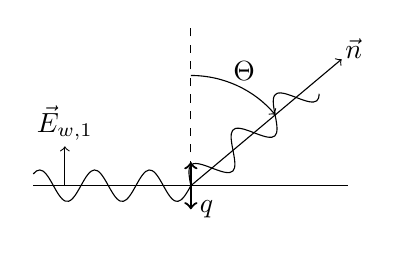
\begin{tikzpicture}
\draw (-2,0) -- (2,0) ;
\draw [dashed] (0,0) -- (0,2);
\draw [<->,thick] (0,-0.3) -- (0,0.3) ;
\draw  (0.2,-0.3) node {$q$};
\draw [->] (0,0) -- (40:2.5) ;
\draw (40:2.7) node {$\vec n$} ;
\draw [->] (90:1.4) arc (90:40:1.4) ;
\draw (65:1.6) node {$\Theta$} ;
\draw [->] (-1.6,0) -- (-1.6,0.5) ;
\draw (-1.6,0.8) node {$\vec E_{w,1}$} ;
\draw plot [domain=-2:0,smooth,samples=50] (\x, {0.2*sin(9*\x r)});
\draw plot [domain=0:2,smooth,samples=50] ({\x*0.7666-0.2*sin(9*\x r)*0.642}, {\x*0.642+0.7666*0.2*sin(9*\x r)});
\end{tikzpicture}
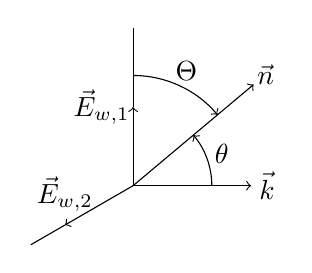
\begin{tikzpicture}
\draw [->] (0,0) -- (-150:1) ;
\draw (-150:1) -- (-150:1.5) ;
\draw (-150:1) ++(0,0.4) node {$\vec E_{w,2}$} ;
\draw [->] (0,0) -- (0:1.5);
\draw (0:1.7) node {$\vec k$} ;
\draw [->] (0,0) -- (90:1) ;
\draw (90:1) ++ (-0.4,0) node {$\vec E_{w,1}$} ;
\draw (90:1) -- (90:2) ;
\draw [->] (0,0) -- (40:2) ;
\draw (40:2.2) node {$\vec n$} ;
\draw [->] (0:1) arc (0:40:1) ;
\draw [->] (90:1.4) arc (90:40:1.4) ;
\draw (65:1.6) node {$\Theta$} ;
\draw (20:1.2) node {$\theta$} ;
\end{tikzpicture}
\caption{Geometry for Thomson scattering}
\end{figure}
}

By averaging over a period of the incident radiation we can derive the
time-averaged power radiated by the charge
\begin{equation}
\frac{dP}{d\Omega} = \frac{q^4 E_0^2}{8\pi m^2 c^3} \sin^2
\Theta~\rmmat{and}~P=\frac{q^4 E_0^2}{3m^2 c^3}
\label{eq:237}
\end{equation}
where $\Theta$ is the angle between the line of sight and the electric
field of the incident radiation.  The incident radiation carries a
flux of $\left \langle S \right \rangle = (c/8\pi) E_0^2$, so we can
define the differential cross section
\begin{equation}
\frac{d \sigma}{d\Omega} = \frac{d P}{d\Omega} \left \langle S \right
\rangle^{-1}=\frac{q^4}{m^2 c^4} \sin^2 \Theta = r_0^2 \sin^2 \Theta
\label{eq:238}
\end{equation}
where $r_0=2.82\times 10^{-13}$~cm for an electron, the classical electron radius.

The total cross section is
\begin{equation}
\sigma = \frac{8\pi}{3} r_0^2 = \sigma_T = 0.665 \times
10^{-24}~\rmmat{cm}^2~\rmmat{for an electron}
\label{eq:239}
\end{equation}

So far we have examined the scattering of polarized radiation.  It is
straightforward to think about scattering of unpolarized radiation by
taking the incoming beam to be a sum of two beams whose polarization
differs by $\pi/2$.
\begin{eqnarray}
\left . \frac{d\sigma}{d\Omega} \right |_\rmscr{unpol} &=& \frac{1}{2}
\left [ \frac{d\sigma(\Theta)}{d\Omega}  +
  \frac{d\sigma(\pi/2)}{d\Omega}  \right ] \\
&=& \frac{1}{2} r_0^2 \left ( 1 + \sin^2 \Theta \right ) = \frac{1}{2}
r_0^2 \left ( 1 + \cos^2 \theta \right ).
\label{eq:240}
\end{eqnarray}
The first term in the expression corresponds to light polarized in the
plane containing ${\bf E}_{w,1}$ and ${\bf n}$ and the second term
traces light polarized in  the
plane containing ${\bf E}_{w,2}$ and ${\bf n}$.   They are two
orthogonal polarizations.   More energy is scattered into the ${\bf
  E}_{w,1}-{\bf n}$ plane than in the other in the ratio of $1:\cos^2
\theta$, so the scattered radiation is polarized with
\begin{equation}
\Pi = \frac{1-\cos^2\theta}{1+\cos^2\theta}
\label{eq:241}
\end{equation}

\section{Radiation Reaction}
\label{sec:radiation-reaction}
\index{electrodynamics!radiation reaction}

We have found that when a charge is accelerated a certain power is
radiated away, so to accelerate the particle we must provide some
extra energy to work against a ``radiation reaction'' force,
\begin{equation}
-{\bf F}_\rmscr{rad} \cdot {\bf u} = \frac{2 q^2 \dot{u}^2}{3 c^3}
\label{eq:242}
\end{equation}
To make sense of this equation, let's consider integrate the power
over a period of time
\begin{equation}
-\int_{t_1}^{t_2} {\bf F}_\rmscr{rad} \cdot {\bf u} dt = \frac{2 q^2 }{3
  c^3} \int_{t_1}^{t_2} \dot{\bf u} \cdot \dot{\bf u} dt = 
\frac{2 q^2 }{3 c^3} \left [ \left . \dot{\bf u} \cdot {\bf u} \right
  |_{t_1}^{t_2} - \int_{t_1}^{t_2} \ddot{\bf u} \cdot \dot{\bf u} dt
  \right ].
\label{eq:243}
\end{equation}
We can drop the term from the endpoints if for example the
acceleration vanishes at $t=t_1$ and $t=t_2$ or if the acceleration
and velocity of the particle are the same at $t=t_1$ and $t=t_2$.  We
can identify,
\begin{equation}
{\bf F}_\rmscr{rad} = \frac{2 q^2}{3 c^3} \ddot{\bf u} = m \tau
\ddot{\bf u}
\label{eq:244}
\end{equation}
where $\tau = 2 r_0/(3 c)$.

\subsection{Radiation from Harmonically Bound Particles}
\label{sec:radi-from-harm}
\index{radiation!bound particles}

We are going to take the results from the previous section to study
particles that are harmonically bound, so their motion satisfies the
following equation,
\begin{equation}
-\tau \dddot{x} + \ddot{x} + \omega_0^2 x = 0
\label{eq:245}
\end{equation}
where the first term contains the radiation reaction.  Let's also
assume that the radiation reaction is only a small perturbation on the
motion so $\dddot{x} \approx -\omega_0 \dot{x}$ and we have
\begin{equation}
\ddot{x} + \omega_0^2 \tau \dot{x} + \omega_0^2 x = 0.
\label{eq:246}
\end{equation}
Let's solve this by assuming that $x(t) = A e^{\alpha t}$.
Substituting and dividing by the exponential yields the characteristic
equation 
\begin{equation}
\alpha^2 +  \omega_0^2 \tau \alpha + \omega_0^2 = 0
\label{eq:247}
\end{equation}
and the solutions
\begin{equation}
\alpha = \pm i \omega_0 \sqrt{1 - \omega_0^2 \tau^2} - \frac{1}{2}
\omega_0^2 \tau.
\label{eq:248}
\end{equation}
To lowest order we can take the square root to be one and we have the
solution
\begin{equation}
x(t) = x_0 e^{-\Gamma t/2} \cos \omega_0 t~\rmmat{where}~\Gamma \equiv
\omega_0^2 \tau = \frac{2 q^2 \omega_0^2}{3mc^3}
\label{eq:249}
\end{equation}
The Fourier transform of this function is
\begin{equation}
{\hat x}(t) = \frac{x_0}{4\pi} \left [ \frac{1}{\Gamma/2 -
    i\left(\omega+\omega_0\right)} + \frac{1}{\Gamma/2 -
    i\left(\omega-\omega_0\right)} \right ]
\label{eq:250}
\end{equation}
If we focus on positive frequencies, the first term is small so we can
approximate the power spectrum of the motion by
\begin{equation}
|{\hat x}|^2 = \left ( \frac{x_0}{4\pi} \right )^2 \frac{1}{(\omega -
  \omega_0)^2 + \left(\Gamma/2\right)^2}.
\label{eq:251}
\end{equation}
and the power radiated per unit frequency is
\begin{eqnarray}
\frac{d W}{d\omega} = \frac{8 \pi \omega^4}{3 c^3}|{\hat d}(\omega)|^2
&=& \frac{8 \pi \omega^4}{3 c^3} \frac{q^2 x_0^2}{(4\pi)^2}  \frac{1}{(\omega -
  \omega_0)^2 + \left(\Gamma/2\right)^2} \\
&=& \left ( \frac{1}{2} k x_0^2 \right ) \frac{\Gamma}{2\pi}\frac{1}{(\omega -
  \omega_0)^2 + \left(\Gamma/2\right)^2}
\label{eq:252}
\end{eqnarray}
The classical line width $\delta \omega=\Gamma$ is a universal
constant for electronic oscillators if expressed as a wavelength
\begin{equation}
\frac{\Delta \lambda}{\lambda} = \frac{\Delta \omega}{\omega}, \Delta
\lambda = \frac{2e^2 \omega_0^2}{3 m c^3} \frac{\lambda}{\omega_0} =  
\frac{4 \pi e^2 }{3 m c^2} = \frac{4\pi}{3} r_0 = 1.2 \times 10^{-12}~\rmmat{cm}
\label{eq:253}
\end{equation}

\subsection{Driven Harmonic Oscillator}
\label{sec:driv-harm-oscill}

Let's imagine that our harmonic oscillator is driven by incoming
electromagnetic wave.  Using the assumptions from the section on
scattering and the radiation reaction we have
\begin{equation}
m \ddot{x} = -m\omega_0^2 x + m \tau \dddot{x} + q E_0 \cos \omega t.
\label{eq:254}
\end{equation}
Let's divide by the mass and take use the exponential for the cosine
\begin{equation}
\ddot{x} -\tau \dddot{x} + \omega_0^2 x = \frac{q E_0}{m} e^{i\omega t}
\label{eq:255}
\end{equation}
and try a solution of the form
\begin{equation}
x = x_0 e^{i\omega t}
\label{eq:256}
\end{equation}
which gives
\begin{equation}
x_0 \left ( -\omega^2 + i \tau \omega^3 + \omega_0^2 \right )= \frac{q E_0}{m} 
\label{eq:257}
\end{equation}
so 
\begin{equation}
x_0 = -\frac{e E_0}{m} \frac{1}{\omega^2-\omega_0^2 - i \tau \omega_0^3}
\label{eq:258}
\end{equation}
It is convenient to express 
\begin{equation}
x_0 = |x_0| e^{i\delta}
\label{eq:259}
\end{equation}
where
\begin{equation}
\tan \delta = \frac{\omega^3\tau}{\omega^2-\omega_0^2}~
\rmmat{and}~|x_0| = \frac{e E_0}{m} 
\left [ \left ( \omega^2-\omega_0^2 \right )^2 + \omega_0^6 \tau^2 \right ]^{-1/2}.
\label{eq:260}
\end{equation}
Let's use the dipole formula to calculate the radiated power
\begin{equation}
P = \frac{q^2 |x_0|^2 \omega^4}{3 c^3} = \frac{q^4 E_0^2}{3m^2 c^3}
\frac{\omega^4}{\left (\omega^2-\omega_0^2\right )^2+\left(\omega_0^3 \tau\right)^2}
\label{eq:261}
\end{equation}
Let's divide by the Poynting vector $\left \langle S \right \rangle =
(c/8\pi) E_0^2$
to get the scattering cross-section
\begin{equation}
\sigma(\omega) = \sigma_T \frac{\omega^4}{\left
  (\omega^2-\omega_0^2\right )^2+\left(\omega_0^3 \tau\right)^2}
\label{eq:262}
\end{equation}
The scattering cross-section has several interesting regimes
\begin{itemize}
\item $\omega \gg\ \omega_0$: $\sigma(\omega) \rightarrow \sigma_T$
\item $\omega \ll\ \omega_0$: $\sigma(\omega) \rightarrow \sigma_T
  \left (\frac{\omega}{\omega_0} \right )^4$
\item $\omega \approx \omega_0$: In this regime it is convenient to
  write 
\begin{equation}
\omega^2 - \omega_0^2 = (\omega - \omega_0) (\omega + \omega_0)
  \approx 2 \omega_0 (\omega-\omega_0)
\label{eq:263}
\end{equation}
and take $\omega=\omega_0$ elsewhere in the cross-section
\begin{equation}
\sigma(\omega) \approx \frac{\pi \sigma_T}{2\tau} 
 \frac{\Gamma}{2\pi}\frac{1}{(\omega -
  \omega_0)^2 + \left(\Gamma/2\right)^2}
\label{eq:264}
\end{equation}
Near the resonance the cross-section has the same profile at the
spontaneous emission.
\end{itemize}

\section{Further Reading}

To learn more about radiation from moving charges, consult Chapter 14
of
\begin{itemize}
\item Jackson, J. D., {\em Classical Electrodynamics}.
\end{itemize}

\section{Problems}

\begin{enumerate}
\item{\bf Constant Velocity Charge}

Show that if charge is not accelerating, the electric field vector
points to the current (not the retarded) position of the charge.

\item{\bf Dipoles:}

Two oscillating dipole moments (radio antennas) ${\bf d}_1$ and ${\bf
d}_2$ are oriented in the vertical direction and are a horizonal
distance $L$ apart.  They oscillate in phase at the same frequency
$\omega$.   Consider radiation at an angle $\theta$ with repect to the
vertical and in the vertical plane containing the two dipoles.

\begin{enumerate}
\item Show that
\[
\frac{dP}{d\Omega} = \frac{\omega^4 \sin^2 \theta}{8 \pi c^3} \left (
d_1^2 + 2d_1 d_2 \cos \delta + d_2^2 \right ),
\]
where
\[
\delta \equiv \frac{\omega L \sin \theta}{c}.
\]
\item Thus show directly that when $L\ll\ \lambda$, the radiation is
  the same as from a single oscillating dipole of amplitude $d_1+d_2$.
\end{enumerate}

\item{\bf Cloud:}

An optically thin cloud surrounding a luminous object is estimate to
be 1 pc in radius and to consist of ionized plasma.  Assume that
electron scattering is the only important extinction mechanism and
that the luminous object emits unpolarized radiation.
\begin{enumerate}
\item If the cloud is unresolved (angular size smaller than the
  angular resolution of the detector), what is the net polarization
  observeed?
\item If the cloud is resolved,  what is the polarization direction of
  the observed radiation as a function of position on the sky?  Assume
  only a single scattering occurs.
\item If the central object is clear seen, what is an upper bound for
  the electron density of the cloud, assuming that the cloud is homogeneous?
\end{enumerate}

\item{\bf Synchrotron Cooling:}

A particle of mass $m$, charge $q$, moves in a plane perpendicular to
a uniform, static, magnetic field $B$.
\begin{enumerate}
\item
Calculate the total energy radiated per unit time, expressing it in
terms of the constants already defined and the ratio
$\gamma=1/\sqrt{1-\beta^2}$ of the particle's total energy to its rest 
energy.  You can assume that the particle is ultrarelativistic.
\item
If at time $t=0$ the particle has a total energy $E_0=\gamma_0 m c^2$,
show that it will have energy $E=\gamma m c^2 < E_0$ at a time $t$,
where
\[
t \approx \frac{3 m^3 c^5}{2 q^4 B^2} \left ( \frac{1}{\gamma} -
\frac{1}{\gamma_0} \right ).
\]
\end{enumerate}

\item{\bf Classical HI:}

A particle of mass $m$ and charge $q$ moves in a circle due to a force 
${\bf F} = -\hat{\bf r} \frac{q^2}{r^2}$.  
You may assume that the particle always moves  non-relativistically.
\begin{enumerate}
\item What is the acceleration of the particle as a function of $r$?
\item What is the total energy of the particle as a function of $r$?
  The potential energy is given by $-q^2/r$.
\item What is the power radiated as a function of $r$?
\item Using the fact the $P=-dE/dt$ and the answer to (b), find
  $dr/dt$. 
\item Assuming that the particle starts with $r=r_i$ at $t=0$, find
  the value of $t$ where $r=0$.   
\item Let's assume that $q=e$, the charge of the electron, and
  $m=m_e$, the mass of the electron.  Write your answer in (d) in
  terms of $r_i$, $r_0$ (the classical electron radius) and $c$.
\item What is the time if $r_i=0.5$\AA\ (for hydrogen)?
\item Compare this to the lifetime of a hydrogen atom.
\end{enumerate}

\item{\bf The Eddington Luminosity:} 

  There is a natural limit to the luminosity a gravitationally bound
  object can emit. At this limit the inward gravitational force on a
  piece of material is balanced by the outgoing radiation
  pressure. Although this limiting luminosity, the Eddington
  luminosity, can be evaded in various ways, it can provide a useful
  (if not truly firm) estimate of the minimum mass of a particular
  source of radiation.

\begin{enumerate}
\item Consider ionized hydrogen gas. Each electron-proton pair has a
  mass more or less equal to the mass of the proton ($m_p$) and a cross
  section to radiation equal to the Thompson cross-section ($\sigma_T$).
\item The radiation pressure is given by outgoing radiation flux over the speed of light.
\item Equate the outgoing force due to radiation on the pair with the inward force of gravity on the pair.
\item Solve for the luminosity as a function of mass.
\end{enumerate}
The mass of the sun is $2 \times 10^{33}$g. What is the Eddington
luminosity of the sun?

\item{\bf The Blue Pool}

Skectch the spectrum of light emitted by an electron with a total
energy of 1~MeV, 3~MeV and 10~MeV travelling through water. 

\end{enumerate}

%%% Local Variables:
%%% TeX-master: "book"
%%% End:

\chapter{Special Relativity}
\label{cha:special-relativity}
\index{special relativity}
\section{Back to Maxwell's Equations}
\label{sec:back-maxw-equat}
Earlier we looked at Maxwell's equations in a vacuum,
\begin{eqnarray}
{\bf \nabla} \cdot {\bf E} = 0 & {\bf \nabla} \cdot {\bf B} =
0 \nonumber \\
{\bf \nabla} \times {\bf E} = -\frac{1}{c} \frac{\partial {\bf
    B}}{\partial t} &
{\bf \nabla} \times {\bf H} = +\frac{1}{c} 
\frac{\partial {\bf D}}{\partial t} 
\label{eq:265}
\end{eqnarray}
and found that they have wave solutions,
\begin{equation}
 {\bf   \nabla}^2 {\bf E}
-\frac{1}{c^2} \frac{\partial^2 {\bf E}}{\partial t^2} = 0
\label{eq:266}
\end{equation}
and a similar equation for the magnetic field.  The waves travel at a
velocity $c$, which turns out to be the speed of light.  The speed of
light had been known approximately since the 1600's (does anyone know
how?). 

Maxwell's and his contemporaries spoke of light travelling through
some medium known as the aether.  Michelson and Morley attempted to
measure the motion of the Earth through the aether, but failed.

Looking at the Michelson-Morley experiment closely shows what is
happening.  Lorentz proposed that to understand the null result of the
experiment objects moving through the aether contract by
$\gamma^{-1}=\sqrt{1-v^2/c^2}$ where $\gamma$ is the Lorentz factor.

Einstein's insight was that if the speed of light was the same for
everyone moving uniformly, one would get the apparent ``Lorentz''
contraction without needing the aether through which light propagates
or for the aether to contract objects.  The aether was originally
proposed by Aristotle and experiments agreed with it for about 2,200
years, so throwing it away was a big deal.

\section{Lorentz Transformations} 
\label{sec:lorentz-transf}
\index{special relativity!Lorentz transformations}

Let's imagine two people moving at a velocity $v$ relative to each
other in the $x$-direction.   Let's also assume that their coordinate
systems coincide at $t=0$, and that one emits a light pulse at
$t=t'=0$ from $x=x'=0$.  After a time has elapsed the light has
reached positions that satisfy,
\begin{equation}
x^2+y^2+z^2 - c^2 t^2 = 0 ~\rmmat{and}~
x'^2+y'^2+z'^2 - c^2 t'^2 = 0.
\label{eq:267}
\end{equation}
We can satisfy these equations if
\begin{eqnarray}
x' &=& \gamma (x-vt) \\
y' &=& y \\
z' &=& z \\
t' &=& \gamma \left ( t - \frac{v}{c^2} x \right )
\label{eq:268}
\end{eqnarray}
and the following inverse relations
\begin{equation}
x = \gamma ( x' + v t'), t=\gamma \left (t'+\frac{v}{c^2} x' \right
)~\rmmat{and the other two equations.}
\label{eq:269}
\end{equation}

\subsection{Length Contraction}
\label{sec:length-contraction}
\index{special relativity!length contraction}

Let's look at the results with the aether again.   If we have a rod of
length $L_0$ in the primed frame what it is length in the unprimed
frame.
\begin{equation}
L_0 = x_2' - x_1' = \gamma ( x_2 - x_1 ) = \gamma L.
\label{eq:270}
\end{equation}
We have define the length to be the extent of an object measured at a
particular time.  Notices that someone in the primed frame would claim
that the person measured the position of one end of the stick at a
different time from the other.

\subsection{Adding velocities}
\label{sec:adding-velocities}
\index{special relativity!adding velocities}

Let's do a final example.  Someone in the primed frame throws a ball
in the $x'$-direction with velocity $u_x'$ from $x'=0$ at $t'=0$, what
velocity will someone measure in the unprimed frame.  After a time
$t'$ the ball will be at $x'=u_x' t'$.  Let's use the inverse
transformation to calculate its coordinates in the unprimed frame,
\begin{equation}
x = \gamma ( u_x' t' + v t' ), t = \gamma \left ( t' + \frac{v}{c^2} u_x'
t' \right ).
\label{eq:271}
\end{equation}
The velocity $u_x$ in the unprimed frame is
\begin{equation}
u_x = \frac{x}{t} = 
\frac{\gamma ( u_x' t' + v t' )}{\gamma \left ( t' + \frac{v}{c^2} t'
  u_x'\right )} = \frac{ u' + v }{1 + v u_x'/c^2}
\label{eq:272}
\end{equation}
If the particle had velocity components in the $y'$ or $z'$ directions
the corresponding components in the unprimed frame are
\begin{equation}
u_y = \frac{y}{t} = 
\frac{\gamma ( u_y' t' )}{\gamma \left ( t' + \frac{v}{c^2} t'
  u_x'\right )} = \frac{ u_y' }{\gamma ( 1 + v u_x'/c^2 )}
\label{eq:273}
\end{equation}
and similarly for the $z$-direction.

The apparent direction of the particle is different in the two frames,
\begin{equation}
\tan \theta = \frac{u_y}{u_x} = \frac{u_y'}{\gamma ( u_x' + v )} =
\frac{u' \sin\theta'}{\gamma ( u' \cos\theta' + v )}.
\label{eq:274}
\end{equation}
This is the aberration equation.  
Let's for an example take $u'=c$ and $\theta'=\pi/2$.   We could
imagine that this is the emission from a dipole moving at a velocity
$v$.  We get
\begin{equation}
\tan \theta = \frac{c}{\gamma v}~\rmmat{or}~\sin\theta = \frac{1}{\gamma}
\label{eq:275}
\end{equation}

\subsection{Doppler Effect}
\label{sec:doppler-effect}
\index{special relativity!Doppler effect}
\index{Doppler effect}
We have a radio transmitter in the primed frame radiating at a
frequency $\omega'$.  According to the time dilation, in the unprimed
frame it oscillates more slowly at a time inverval 
$\Delta t=2\pi \gamma/\omega$.. The
time between the arrival for two crests of the wave in the unprimed
frame is  given by,
\begin{equation}
\Delta t_A = \Delta t - \frac{d}{c} = \Delta t \left (  1 -
\frac{v}{c} \cos\theta \right ).
\label{eq:276}
\end{equation}
so
\begin{equation}
\omega = \frac{2 \pi}{\Delta t_A} = \frac{\omega'}{\gamma \left (  1 -
\frac{v}{c} \cos\theta \right )}
\label{eq:277}
\end{equation}

\section{Four-Vectors}
\label{sec:four-vectors}
\index{special relativity!four-vectors}
\index{four-vectors}

We have found many strange properties of special relativity in a
rather {\em ad hoc} manner.  All of these properties resulted from the
fact that
\begin{equation}
s^2 = -c^2 \tau^2 = -c^2 t^2 + x^2 + y^2 + z^2
\label{eq:278}
\end{equation}
is the same for all observers travelling uniformly relative to each
other.   In three dimensions we can think about vectors whose length
$x^2+y^2+z^2$ is invariant with respect to rotations.  Once we
establish that a certain quantity is a vector we can use the
transformation properties of the vectors under rotation to determine
what its value is in any other frame.

Similarly in relativity, it is convenient to define something called a
four-vector whose components transform between rotated frames and
frames moving at different velocities such that the equation above
holds.  A four vector is simply
\begin{equation}
x^\mu = \left [ \begin{array}{c} ct \\ x\\ y\\ z \end{array} \right ]
\label{eq:279}
\end{equation}
and 
\begin{equation}
s^2 = \sum_{\mu=0}^3 \sum_{\nu=0}^3 \eta_{\mu\nu} x^\mu x^\nu \equiv
\eta_{\mu\nu} x^\mu x^\nu \equiv  x^\mu x_\mu 
\label{eq:280}
\end{equation}
where
\begin{equation}
\eta_{\mu\nu} = \eta^{\mu\nu} = \left [ 
\begin{array}{rrrr}
-1 & 0 & 0 & 0 \\
 0 & 1 & 0 & 0 \\
 0 & 0 & 1 & 0 \\
 0 & 0 & 0 & 1 
\end{array}
\right ]
~\rmmat{and}~
x_\mu = \left [ -ct~x~y~z \right ].
\label{eq:281}
\end{equation}
This tensor $\eta_{\mu\nu}$ defines the metric for flat spacetime.  It
is called the metric because you need it to convert various four
vectors (and other objects tensors) into scalars that we can measure.
We have selected the particular convention that time-time component is
negative (like in Misner, Thorne and Wheeler).  Jackson use the
opposite convention.  If the index is upstairs the vector is
contravariant and if it is downstairs it is convariant.

Now we can write the transformation between two frames very concisely
\begin{equation}
x'^\mu = \Lambda^\mu_{~\nu} x^\nu
\label{eq:282}
\end{equation}
where
\begin{equation}
\Lambda^\mu_{~\nu} = \left [ 
\begin{array}{rrrr}
\gamma      & -\beta \gamma  & 0 & 0 \\
-\beta\gamma &         \gamma & 0 & 0 \\
          0 &             0  & 1 & 0 \\
          0 &             0  & 0 & 1 
\end{array}
\right ]
\label{eq:283}
\end{equation}
This matrix looks remarkably similar to a rotation matrix.  For
example,
\begin{equation}
A = \left [ 
\begin{array}{rrrr}
\cos \theta & -\sin\theta   & 0 & 0 \\
\sin\theta &  \cos\theta & 0 & 0 \\
          0 &             0  & 1 & 0 \\
          0 &             0  & 0 & 1 
\end{array}\right ] 
\label{eq:284}
\end{equation}
This is no coincidence.  A boost (shift between frames with two
different velocities) is like a rotation in spacetime.  However,
we have in the rotation case we have
\begin{equation}
\cos^2\theta + \sin^2\theta = 1
\label{eq:285}
\end{equation}
while in the boost case we have
\begin{equation}
\gamma^2 - (\beta\gamma)^2 = \gamma^2 ( 1 - \beta^2 ) = 1.
\label{eq:286}
\end{equation}
Sometimes people define the rapidity $\zeta$ such that $\gamma = \cosh
\zeta$.  The nice thing about the rapidity is that like the angle
$\theta$ it is additive for successive boosts.

What about the transformation of the covariant vector?
\begin{equation}
s^2 = x^\mu x_\mu = x'^\alpha x'_\alpha = \Lambda^\alpha_\mu 
{\tilde \Lambda}_\alpha^\nu  x^\mu x_\nu
\label{eq:287}
\end{equation}
which tells us that
\begin{equation}
\Lambda^\alpha_\mu 
{\tilde \Lambda}_\alpha^\nu  = \delta^\nu_\mu
\label{eq:288}
\end{equation}
so the covariant vector transforms using the inverse matrix.

Let's try to find some physically meaningful four-vectors.    We know
that a displacement is a four-vector.  Let's try to find a four-vector
related to the velocity of a particle.
\begin{equation}
U^\mu = \frac{d x^\mu}{d t^?}
\label{eq:289}
\end{equation}
The numerator is a displacement that transforms as a four-vector.  For
the left-hand side also to be a four-vector the denominator must be
the same in all frames (a Lorentz scalar).  The only one is $d\tau$
which we defined earlier.  This is the time measured by someone moving
with the particle.  We have
\begin{equation}
U^\mu = \gamma_u \left [ \begin{array}{c} c \\ u_x \\ u_y \\ u_z \end{array} 
    \right ] = \gamma_u \left [ \begin{array}{c} c \\ {\bf u}
  \end{array} \right ]
\label{eq:290}
\end{equation}
What this means is that for each second measured by someone moving
with the particle, $\gamma$ times one second elapses for us and the
particle travels $\gamma {\bf u}$ times one second.

What is the magnitude of $U^\mu$?   
\begin{equation}
U^\mu U_\mu = -\left (\gamma_u c\right)^2 - \left ( \gamma_u {\bf u}
\right )^2 = -c^2 \gamma_u^2 \left ( 1 - \beta^2 \right ) = -c^2 
\label{eq:291}
\end{equation}
If a particle is at rest its four-velocity is given by
$U^0=c$ and $U^i=0$.  

In non-relativistic mechanics, we define the momentum to be the mass
times the velocity, similarly we can define the four-momentum to 
$p^\mu = m U^\mu$.  Let's look at the properties of this vector in
more detail.  Its components are
\begin{equation}
p^\mu = \gamma_u m \left [ \begin{array}{c} c \\ u_x \\ u_y \\ u_z \end{array} 
    \right ] = \left [ \begin{array}{c} \gamma_u m c \\ {\bf p}
  \end{array} \right ]
\label{eq:292}
\end{equation}
Let's expand the first component to see what it is
\begin{eqnarray}
p_t &=& \gamma_u m c = \left (1 - \frac{v^2}{c^2} \right )^{-1/2} m c \approx
 m c + \frac{1}{2} m \frac{v^2}{c} \\
    &=& \frac{m c^2 + \rmmat{KE}}{c} = \frac{E}{c} \\
\label{eq:293}
\end{eqnarray}
If we calculate $p^\mu p_\mu$ we find the relativistic relationship
between energy and momentum 
\begin{eqnarray} 
p^\mu p_\mu &=& -(m c)^2 =  {\bf p}\cdot {\bf p} - \frac{E^2}{c^2} \\
E &=& \sqrt{c^2 p^2 + m^2 c^4}
\label{eq:294}
\end{eqnarray}

Another important four-vector shows up in the equation for the
propagation of an electromagnetic wave.  The electric and magnetic
fields of the wave are proportional to $\cos ({\bf k}\cdot {\bf x} -
\omega t)$.  If both fields vanish at a point and time in spacetime,
all observers should agree on this regardless of their motion so 
\begin{equation}
{\bf k}\cdot {\bf x} - \omega t = k_\mu x^\mu 
\label{eq:295}
\end{equation}
is a scalar. Because $x^\mu$ is a four-vector, 
\begin{equation}
k^\mu = \left [ \begin{array}{c}
\omega/c \\ {\bf k} \end{array} \right ]
\label{eq:296}
\end{equation}
must be one as well.
This leads to a quick way to derive the redshift formula.  The person
observing a wave finds 
\begin{equation}
-\omega' = k^\mu U'_\mu = -\gamma \left (
\omega - {\bf k}\cdot {\bf u} \right ) = -\gamma \omega \left ( 1 -
\frac{v}{c}\cos\theta\right ) 
\label{eq:297}
\end{equation}

\section{Tensors}
\label{sec:tensors}
\index{special relativity!tensors}
\index{tensors}

We have essentially stumbled upon a few nice four-vectors, but there
is a more systematic way of dealing with four-vectors, scalars and
other quantities like the transformation matrix $\Lambda^\mu_{~\nu}$.
All of these objects are examples of tensors.

We can work out how tensors transform by looking at a few examples.  
The quantity
\begin{equation}
T^{\mu\nu} = A^{\mu} B^{\nu}
\label{eq:298}
\end{equation}
is a tensor.  Let's use the Lorentz matrix to transform to a new frame
\begin{equation}
T'^{\alpha\beta} = A'^{\alpha} B'^{\beta} = \Lambda^\alpha_{~\mu} A^{\mu}
\Lambda^\beta_{~\nu} B^{\nu} = \Lambda^\alpha_{~\mu} 
\Lambda^\beta_{~\nu} T^{\mu\nu}.
\label{eq:299}
\end{equation}
We can find similar results for mixed tensors and covariant tensors.

Right now, we can build a contravariant vector by taking a set of
coordinates $x^i$ for a event in spacetime and we can construct a
covariant vector by applying the metric $\eta_{\mu\nu}$ to lower the
index of the vector.  How else can we make a covariant vector?

Let's say there is a scalar field defined over all spacetime.  This just means a 
Lorentz invariant number at each point and time.   We could ask how much this number 
changes as one goes from one event in spacetime to another:
\begin{equation}
\Delta f = f \left (x^{\mu} + \Delta x^\mu \right) -  f \left (x^{\mu}\right)
\label{eq:300}
\end{equation}
The quantity on the left is clearly a scalar because it is the
different in the value of a scalar field at two points.  Let's imagine that we take
$\Delta x^\mu$ to be really smaller so that $\Delta f$ is proportional to 
$\Delta x^\mu$ then we have
\begin{equation}
\Delta f = \frac{\partial f}{\partial x^{\mu}} \Delta x^\mu \equiv f_{,\mu} \Delta x^\mu
\label{eq:301}
\end{equation}
Because $\Delta x^\mu$ transforms as a contravariant vector and $\Delta f$ doesn't 
transform, $f_{,\mu}$ must transform as a covariant vector.

We could also imagine taking the derivative of the vector field to create a tensor, 
for example,
\begin{equation}
A^{\mu}_{,\nu} = \frac{\partial A^\mu}{\partial x^{\nu}}
\label{eq:302}
\end{equation}
If we take $A^{\mu}$ to be the vector potential plus the scalar
potential,
\begin{equation}
A^\mu = \left [ \begin{array}{c}
\phi \\ {\bf A} \end{array} \right ],
\end{equation}
we have
\begin{equation}
\partial_\nu \partial^\nu A^{\mu} = \frac{4 \pi}{c} J^\mu~\rmmat{and}~\partial_\alpha A^\alpha = 0 
\label{eq:303}
\end{equation}
gives the equations of electrodynamics in the Lorenz gauge, where
\begin{equation}
J^\mu = \left [ \begin{array}{c}
c \rho \\ {\bf J} \end{array} \right ].
\end{equation}

We have argued that we can only measure the fields themselves, so we
would like to figure out how the fields transform.  Under rotations
the fields act like vectors.  Can we generalize the electric and
magnetic field to be four-vectors?

The answer is no.   Let's take a look at definitions of the 
fields in terms of the potentials,
\begin{eqnarray}
{\bf E} &=&  - \nabla \phi -\frac{1}{c} \pp{\bf A}{t} \\
{\bf B} &=& \nabla \times {\bf A}
\label{eq:304}
\end{eqnarray}
Let's look at the $x-$components of the fields 
\begin{eqnarray}
E_x &=& - \pp{\phi}{x} -\frac{1}{c} \pp{A_x}{t} = A_{0,1} - A_{1,0} \\
B_x &=& \pp{A_z}{y} - \pp{A_y}{z} = A_{3,2} - A_{2,3} 
\label{eq:305}
\end{eqnarray}
so the electric and magnetic fields seem to be the components of the second rank tensor,
\index{special relativity!field tensor}
\begin{equation}
F_{\alpha\beta} = -\left ( A_{\alpha,\beta} - A_{\beta,\alpha} \right ) = \left [
\begin{array}{cccc} 
0   & -E_x & -E_y & -E_z \\
E_x &    0 &  B_z &  -B_y \\
E_y & -B_z &   0  &  B_x \\
E_z &  B_y &  -B_x &  0
\end{array}
\right ] 
\label{eq:306}
\end{equation}
where the index $\alpha$ labels the rows and $\beta$ labels the columns.
Let's look first at the Lorentz force equation,
\begin{equation}
\dd{\bf p}{t} = q \left ( {\bf E} + \frac{\bf v}{c} \times {\bf B} \right )
\label{eq:307}
\end{equation}
To generalize this we know that ${\bf p}$ transforms as the space-part
of the four-vector $p^\mu$.  We also need to use the proper time $\tau$ instead of the 
coordinate time $t$, this gives
\begin{equation}
\dd{\bf p}{\tau} = \frac{q}{c} \left ( U_0 {\bf E} + {\bf U} \times {\bf B} \right )
\label{eq:308}
\end{equation}

\paragraph{Something to think about.}
Why did the velocity terms on the right-hand side become four velocities?

We also need an equation for the time-like component of the four-momentum.
\begin{equation}
\dd{p_t}{\tau} = \frac{q}{c} {\bf U} \cdot {\bf E}.
\label{eq:309}
\end{equation}
We can combine these equations into a single equation using the field tensor,
\begin{equation}
\dd{p^\alpha}{\tau} = m \dd{U^\alpha}{\tau} = \frac{q}{c} F^{\alpha}_{~~\beta} U^\beta
\label{eq:310}
\end{equation}
or
\begin{equation}
\frac{d}{d\tau}
\left [ \begin{array}{c}
E \\
p_x \\
p_y \\
p_z
  \end{array}
  \right ]
= \frac{\gamma q}{c} \left [ 
\begin{array}{cccc}
0   & E_x & E_y & E_z \\
E_x &  0  & B_z & -B_y \\
E_y & -B_z &  0  & B_x \\
E_z & B_y & -B_x &  0
  \end{array}
\right ]
 \left [ \begin{array}{c}
     c \\
     v_x \\
     v_y \\
     v_z 
  \end{array}
\right ]
\end{equation}
which defines the field tensor without reference to the potentials.
The timelike components of this mixed tensor are not antisymmetric but
it does have the advantage that its components are independent of the
signature that you are using.

Similarly Maxwell's equations can be written in the compact form
\begin{equation}
F^{\alpha\beta}_{~~,\beta} = \frac{4\pi}{c} J^\alpha~\rmmat{and}~{\cal F}^{\alpha\beta}_{~~,\beta} = 0
\label{eq:311}
\end{equation}
where 
\begin{equation}
{\cal F}^{\alpha\beta} = \frac{1}{2} \epsilon^{\alpha\beta\gamma\delta}F_{\gamma\delta} = \left [
\begin{array}{cccc} 
0   & -B_x & -B_y & -B_z \\
B_x &    0 & E_z &  -E_y \\
B_y & -E_z  &   0  & E_x \\
B_z & E_y &  -E_x &  0
\end{array}
\right ] 
\label{eq:312}
\end{equation}
To construct ${\cal F}^{\alpha\beta}$ from $F^{\alpha\beta}$ we put
${\bf E}\rightarrow {\bf B}$ and ${\bf B}\rightarrow-{\bf E}$.  This
is called a duality transformation.

\section{Transformation of Radiative Transfer}
\label{sec:transf-radi-transf}
\index{special relativity!radiative transfer}
The equations of radiative transfer follow the intensity of the
radiation field.  We would like to understand how this and other
radiative transfer quantities transform relativistically.

As I argued earlier, the intensity of a radiation field is related to
the phase space density of photons.  Phase space density is simply the
number of particles in a certain range of momenta in a particular
location,
\begin{equation}
f = \frac{d N}{d^3 {\bf p}' d^3 {\bf x}'}.
\label{eq:313}
\end{equation}
We would like to see how $f$ transforms relativistically.   First the
numerator is simply the number of particles in the region of phase
space that we can count and all should agree upon.   The second term
in the denominator is the volume that the particles occupy.  Let's
assume that the primed frame is moving a velocity $\beta c$ in the
$x-$direction relative to the unprimed frame.  For convenience let's
assume that the origins of the two coordinate systems coincide at
$t=t'=0$.  These assumptions cover all of the possibilities because
the volumes $d^3 {\bf x}$ and $d^3 {\bf p}$ are invariant under
rotations.  The following derivation follows one by Jeremy Goodman.
We will take $c=1$ to simply the proof.

First let's write momenta in the primed frame in terms of its values
in the unprimed frame, we have
\begin{eqnarray}
p'_t &=& \gamma \left ( p_t - \beta p_x \right ) \\
p'_x &=& \gamma \left ( p_x - \beta p_t \right ) \\
p'_y &=& p_y \\
p'_z &=& p_z .
\end{eqnarray}
Now let's construct the Jacobian of the transformation,
\begin{equation}
\left | \begin{array}{ccc}
\frac{\partial  p'_x}{\partial p_x} & \frac{\partial  p'_x}{\partial p_y} & \frac{\partial 
p'_x }{ \partial p_z} \\
\frac{\partial  p'_y}{\partial p_x} & \frac{\partial  p'_y}{\partial p_y} & \frac{\partial 
p'_z }{ \partial p_z} \\
\frac{\partial  p'_z}{\partial p_x} & \frac{\partial  p'_z}{\partial p_y} & \frac{\partial 
p'_z }{ \partial p_z }
  \end{array}
\right | =
\left | \begin{array}{ccc}
\gamma \left ( 1 - \beta \frac{\partial  p_t}{\partial p_x } \right ) & -\gamma
\beta \frac{\partial  p_t}{\partial p_y} & -\gamma \beta \frac{\partial 
p_t }{ \partial p_z} \\
0  & 1 & 0 \\
0 & 0 & 1 
  \end{array}
\right |
\end{equation}
yielding the value of the Jacobian,
\begin{equation}
\gamma \left ( 1 - \beta \frac{\partial p_t}{\partial p_x} \right ).
\end{equation}
Now we can calculate $\partial p_t/\partial p_x$ from the relationship
between the four momentum and mass
\begin{equation}
p_t^2 - {\bf p}^2 = m^2
\end{equation}
so $\partial p_t/\partial p_x=p_x/p_t$ and the Jacobian is
\begin{equation}
\gamma \left ( 1 - \beta \frac{p_x}{p_t} \right ) =
\frac{\gamma \left ( p_t - \beta p_x \right )}{p_t} = \frac{p_t'}{p_t}.
\end{equation}
so 
\begin{equation}
d^3 {\bf p}' = \frac{p_t'}{p_t} d^3 {\bf p} ~\textrm{so}~
\frac{ d^3 {\bf p}}{p_t} ~\textrm{is invariant.}
\end{equation}
Now let's look at the transformation of the length interval $dx$.
Let's take two particles travelling at the same velocity but separated
by some distance. First in the primed frame we have
\begin{equation}
x'_A = v' t_A' + x'_A(0), x'_B = v' t_B' + x'_B(0).
\end{equation}
To measure the distance between them in the primed frame we take
$t'_A=t'_B$ so $\Delta x'=x'_A(0)-x'_B(0)$.  Let's substitute the
values of $x'_A$ and $t'_A$ in terms of $x_A$ and $t_A$ to yield
\begin{equation}
\gamma \left (x_A - \beta t_A \right ) = v' \gamma \left (t_A - \beta x_A\right )
+ x_A(0)
\end{equation}
and solving for $x_A$ yields
\begin{equation}
x_A = \frac{\beta + v'}{1+\beta v'} t_A + \frac{x_A'(0)}{\gamma \left (1 +
  \beta v'\right )}.
\end{equation}
Notice how the particle travels at a different velocity in the new
frame and the relativistic addition of velocities.  Now we find that
\begin{equation}
\Delta x = \frac{\Delta x'}{\gamma \left (1 +
  \beta v'\right )}. 
\end{equation}
Looking at the denominator, we have
\begin{equation}
\gamma \left ( 1 + \beta v' \right ) =  \frac{\gamma\left ( p'_t + \beta p'_x
\right ) }{p'_t} = \frac{p_t}{p'_t}
\end{equation}
where we have used $v'=p'_1/p'_t$ and the inverse Lorentz
transformation, so we find
\begin{equation}
\Delta x = \Delta x' \frac{p'_t}{p_t} 
 ~\textrm{so}~
p_t d^3 {\bf x} ~\textrm{is invariant.}
\end{equation}
% We know that
% \begin{equation}
% dx=\gamma^{-1} dx', dy=dy', dz=dz'
% \label{eq:314}
% \end{equation}
% so the volume in the second frame is smaller by a factor of $\gamma$
% due to the Lorentz contraction,
% \begin{equation}
% d^3 {\bf x} = \gamma^{-1} d^3 {\bf x}'
% \label{eq:315}
% \end{equation}
% Let's imagine in the primed frame that the mean momentum of the
% photons ${\bf p}'$ is small compared to the spread in the momenta
% $d{\bf p}'$.  Let's calculate the spread in the value of $dp^0$.
% \begin{eqnarray}
% (p'^0 + dp'^0)^2 - ({\bf p}' + d {\bf p}' )^2 &=& 0 \\
% (p'^0)^2 + 2 dp'^0 p'^0 + (dp'^0)^2 - {\bf p}'^2 - 2{\bf p}' \cdot d {\bf p}'
% - d{\bf p}'^2 &=& 0 \\
% 2 dp'^0 p'^0 + (dp'^0)^2 - \left( d{\bf p}'^2 \right ) &=&0 .
% \label{eq:316}
% \end{eqnarray}
% The final equation shows that the $dp'^0$ is second order so we can
% neglect it in what follows. Now let's calculate the components of the
% momentum in the unprimed frame,
% \begin{equation}
% dp_y' d p_z' = dp_y dp_x ~\rmmat{and}~ dp_x = \gamma \left (dp_x' +
% \beta dp_t' \right ), dp_x = \gamma d p_x'
% \label{eq:317}
% \end{equation}
% so we have
% \begin{equation}
% d^3 {\bf p} d^3 {\bf x} = \gamma d^3 {\bf p}' \gamma^{-1} d^3 {\bf x}'
% = d^3 {\bf p}' d^3 {\bf x}'
% \label{eq:318}
% \end{equation}
Therefore, $d^3 {\bf x} d^3 {\bf p}$ is Lorentz invariant and
\begin{equation}
f = \frac{d N}{d^3 {\bf p}' d^3 {\bf x}'}. = \frac{d N}{d^3 {\bf p}
  d^3 {\bf x}},
\label{eq:319}
\end{equation}
phase-space density is a Lorentz invariant.

Let's calculate the energy density of the photon field,
\begin{eqnarray}
h\nu f d^3 {\bf p} = h \nu f p^2 dp d\Omega &=& u_\nu (\Omega) d\Omega
d\nu \\
h\nu f \left (\frac{h\nu}{c} \right )^2 d \left (\frac{h\nu}{c}\right
) d\Omega &=& \frac{I_\nu}{c} d \Omega d\nu \\
h^4 \nu^3 c^{-3} f d\nu d\Omega &=& \frac{I_\nu}{c} d \Omega d\nu \\
\frac{h^4}{c^2} f d\nu d\Omega &=& \frac{I_\nu}{\nu^3} d\nu d\Omega
\label{eq:320}
\end{eqnarray}
Because the left-hand side is a bunch of Lorentz invariants we find
that
\begin{equation}
\frac{I_\nu}{\nu^3} = \rmmat{Lorentz invariant}
\label{eq:321}
\end{equation}
A second more heuristic way to find this result is to focus on the
intensity of  blackbody radiation
\begin{equation}
I_\nu = B_\nu(T) = \frac{2 h}{c^2} \frac{\nu^3}{\exp ( h \nu / k T) - 1}.
\end{equation}
To preserve the shape of the blackbody function, the ratio $h \nu/k T$
should be invariant with boosts.  The constants, $h$ and $c$, must
also be invariant, so we have
\begin{equation}
\frac{I_\nu}{\nu^3} = \frac{B_\nu(T)}{\nu^3} = \frac{2 h}{c^2}
\frac{1}{\exp ( h \nu / k T) - 1} = \rmmat{Lorentz invariant}.
\end{equation}
Because the source function $S_\nu$ appears in the equations of
radiative transfer as $I_\nu - S_\nu$, $S_\nu$ must have the same
transformation properties as $I_\nu$, {\em i.e.}
\begin{equation}
\frac{S_\nu}{\nu^3} = \rmmat{Lorentz invariant}
\label{eq:322}
\end{equation}
The optical depth $\tau$ is simply the logarithm of the fraction of
radiation that remains after passing through a slab of absorbing
material we have
\begin{equation}
\tau = \frac{l \alpha_\nu}{\sin \theta} = \frac{l}{\nu \sin \theta}
\nu \alpha_\nu = \frac{l c}{k_y} \nu \alpha_\nu = \rmmat{Lorentz invariant}
\label{eq:323}
\end{equation}
If we move relative to the slab in the $x-$direction, the thickness of
the slab in the $y-$direction, $l$, does not change.  Although $\nu$
and $\sin \theta$ will change, $k_y$ will not change because it is not
in the direction of the motion, so we have
\begin{equation}
\nu \alpha_\nu = \rmmat{Lorentz invariant}
\label{eq:324}
\end{equation}
Finally, we have $j_\nu = \alpha_\nu S_\nu$, so
\begin{equation}
\frac{j_\nu}{\nu^2} = \rmmat{Lorentz invariant}
\label{eq:325}
\end{equation}
These relations allow us to calculate the radiative transfer 
through a medium in whichever frame is convenient.  We could calculate
the source function and absorption in the rest-frame of the material 
and the radiative transfer in the ``lab'' frame.  Or we could
calculate everything in the rest frame and translate the intensity
to the ``lab'' frame.

\section{Further Reading}

To learn more about special relativity, consult Chapter 12
of
\begin{itemize}
\item Jackson, J. D., {\em Classical Electrodynamics}.
\end{itemize}
Please note that Jackson uses the opposite signature to here, so some
formulas may differ.

\section{Problems}

\begin{enumerate}
\item{\bf The Ladder and the Barn: A Spacetime Diagram:}

This problem will work best if you have a sheet of graph paper.
In a spacetime diagram one draws a particular coordinate (in our case
$x$)  along the horizontal direction and the time coordinate
vertically.  People also generally draw the path of a light ray at
45$^\circ$.  This sets the relative units of the two axes.
\begin{enumerate}
\item Draw a spacetime diagram and label the axes $x$ and
  $t$.  The $t$-axis is the path of Emma through the spacetime.

\item Draw the world line of someone travelling at
  $\frac{3}{5}$ of the speed of light.  The world line should
  intersect with the origin of the spacetime diagram.  Label this
  world line $t'$.  The $t'$-axis is the path of Kara through the
  spacetime. 

\item Draw the $x'$ axis on the graph.   Here's a hint about
  where it should go.   The light ray bisects the angle between the
  $x$ and $t$ axes.  Kara who is travelling along $t'$ will find that
  the speed of light is the same for her, so the light ray must also
  bisect the angle between $x'$ and $t'$.

\item Parallel to Emma's time axis draw the walls of the barn
  in pencil.  The barn is 4.5 meters wide in Emma's frame.

\item Draw Kara's ladder along Kara's $x$-axis.   The ladder
is 5 meters long in Kara's frame.  How long is it in Emma's frame.

\item Draw the world lines of the ends of Kara's ladder.
These lines are parallel to Kara's time axis.

\item Erase a portion of the barn walls to allow Kara's ladder
  to fit through.   

\item Using the diagram, explain how Kara and Emma can
  understand how the too-long ladder fits in the too-small barn.
\end{enumerate}

\item{\bf The Fermi Process:}

One model to understand how cosmic rays are accelerated is through
shocks. The main idea is that a charge particle can cross a shock and
turned around by the tangled mangetic field and recross the shock.
Each time the charge does this it gains energy.   

To understand this let's use a simplified model in which two mirrors
are travelling toward each other at some velocity $v$.  When a
particle hits the mirror, its energy in the frame of the mirror
remains unchanged but its velocity and therefore the spacelike
components of the four-momentum change sign.
\begin{enumerate}
\item Draw a diagram with the two mirrors.

\item For argument's
sake, let's first focus on the mirror on the left and consider that
the mirror on the right is moving.   What is the four-velocity in this
frame of the mirror on the left ($U_{l}^\mu$)?  What is the four-velocity in this
frame of the mirror on the right ($U_{r}^\mu$)?

\item Now let's focus on the mirror on the right and consider that
the mirror on the left is moving.  What is the four-velocity in this
frame of the mirror on the left ($U'^\mu_l$)?  What is the
four-velocity in this frame of the mirror on the right ($U'^\mu_r$)?

\item To start let's assume that the particle of mass $m$
  approaches the mirror on the left at the velocity of the mirror on
  the right.  What is the four-momemtum of the particle ($p^\mu$) in
  the frame of the mirror on the left?

\item The particle bounces off of the mirror.  What is its
  four-momentum now?

\item Now the particle is approaching the mirror on the
  right.  What is the zeroth component of the four-momentum of the
  particle in the frame of the right-hand mirror?   One could do a
  Lorentz transformation but it is easier to use $U^\mu_r p_\mu$ to
  determine the energy of the particle in the primed frame.

\item Using the answer to 6, construct the four-momentum of
  the particle in the frame of the right-hand mirror ($p'_\mu$).

\item The particle bounces off of the mirror.  What is its
  four-momentum now?

\item Now the particle is approaching the mirror on the
  left.  What is the zeroth component of the four-momentum of the
  particle in the frame of the left-hand mirror?   Again one could 
  do a Lorentz transformation but it is easier to use $U'^\mu_l p'_\mu$ to
  determine the energy of the particle in the unprimed frame.

\item Compare the energy of the particle in step (d) to the
  energy of the particle in step (i).  Has the energy of the particle
  increased?  Let's let the relative velocity of the mirrors approach
  the speed of light.
$$
\beta \approx 1 - \frac{1}{2\gamma^2}
$$
  By what factor does the energy of the particle increase each time it
  goes back and forth.

\item  The final element is the fact that only a tiny
  fraction of the particles bounce back and forth.  Let's take that
  fraction to be $10^{-5}$ and $\gamma=100$.  What can you say about
  the final distribution of particle energies?

\end{enumerate}
\item{\bf Boosting}
We are going to figure out how times and energies measured by someone in motion differ from what we might measure.
\begin{enumerate}

\item Use special relativity (the Minkowski metric) to figure this
  out. I measure a photon to have an energy $E$. What is the
  four-momentum of the photon?

\item My pal is travelling toward me in the opposite direction of the
  photon at a velocity $\beta c$. What is his four-velocity? Use the
  definition $\gamma = \left ( 1- \beta^2\right)^{-1/2}$ to simplify
  the expression. What energy would he measure for the photon? What
  does the expression look like as $\gamma$ gets much larger than one?

\item If my pal observes the photon to have an energy of 100~MeV while
  I say its energy is less than 500~keV, what is the minimal value of
  $\gamma$ for my pal (take $\beta \approx 1$ to make life easier)?

\item My pal is still coming toward me at a velocity $\beta c$. When
  he is a distance $r$ away from me (at a time $t_0$) he emits a photon
  toward me. How long does it take this photon to reach me?

\item From his point of view a short time $\Delta t$ later he emits
  another photon toward me. How long is $\Delta t$ in my frame and
  when do I receive the second photon? What is the difference in time
  between when I receive the first and second photons? What does the
  expression look like as $\gamma$ gets much larger than one? Compare
  it with you answer to (b).
\end{enumerate}

\item{\bf Precession}
We will calculate the transformation that results from a pair of
boosts in different directions.
\begin{enumerate}
\item Write out the Lorentz transformation matrix for a boost in the
  $x-$direction to a velocity $\beta_x$.
\item Write out the Lorentz transformation matrix for a boost in the
  $y-$direction to a velocity $\beta_y$.
\item
  Write out the Lorentz transformation matrix for a boost in the
  $x-$direction to velocity $\beta_x$ followed by boost to a velocity
  $\beta_y$ in the $y-$direction.
\item
  Write out the Lorentz transformation matrix for a boost in the
  $x-$direction to velocity $\beta_x$, followed by boost to a velocity
  $\beta_y$ in the $y-$direction, followed a boost in the
  $x-$direction to velocity $-\beta_x$ followed by boost to a velocity
  $-\beta_y$ in the $y-$direction.  
\item Now you have undone both boosts and have zero velocity, did you
  get the identity?  Why or why not?
\end{enumerate}

\end{enumerate}
%%% Local Variables:
%%% TeX-master: "book"
%%% End:
\chapter{Bremsstrahlung}
\label{cha:bremsstrahlung}
\index{bremsstrahlung}
Bremsstrahlung or braking radiation is the radiation that the charged
particle emits while being accelerated in the electric field of
another particle.  Because the amount of radiation produced is
proportional to the square of the acceleration, the less massive
particle generally dominates the emission.  Typically, we are talking
about an electron and an ion, so the mass ratio is greater than 1,800
to one.

Why is it called bremsstrahlung?  X-rays were first produced in the
laboratory by accelerating electrons along a strong electric field (a
typical potential difference of 10kV) from an anode to a cathode in
vacuum.  When the electrons hit the thick metal cathode and stop
(brake), they emit cathode rays or X-rays.

\section{The Physics of Bremsstrahlung}
\label{sec:phys-bremsstr}

If we ignore the effect of radiation reaction of the trajectory of the
charged particle, we can solve for its path exactly (at least in the
classical limit) and then use the formulae for the radiation field
that we derived a few weeks back.   You can check out the Padmanabhan
text if you would like to see an exact treatment.

\paragraph{Something to think about.}  What is the exact classical 
trajectory of the charged particle?  

We will approximate the exact trajectories shown in the left-hand
panel of Fig.~1 by a simple straight line trajectory in which the
acceleration of the particle lies mainly normal to the direction of the
particle's motion.
{
\begin{figure}
\centering
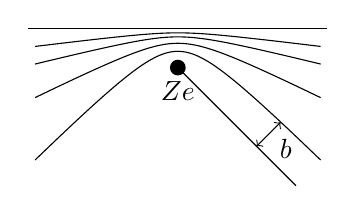
\begin{tikzpicture}
\draw plot [domain=-2:2,smooth] ({(exp(-\x)-exp(\x))/4}, {(-exp(\x)-exp(-\x))/4});
\draw plot [domain=-2:2,smooth] ({(exp(-\x)-exp(\x))/4}, {(-exp(\x)-exp(-\x))/8+sqrt(1/4+1/16)-sqrt(0.5)});
\draw plot [domain=-2:2,smooth] ({(exp(-\x)-exp(\x))/4}, {(-exp(\x)-exp(-\x))/16+sqrt(1/4+1/64)-sqrt(0.5)});
\draw plot [domain=-2:2,smooth] ({(exp(-\x)-exp(\x))/4}, {(-exp(\x)-exp(-\x))/32+sqrt(1/4+1/256)-sqrt(0.5)});
\draw (-1.9,-0.2071067812) -- (1.9,-0.2071067812) ;
\fill (0,-0.707) circle (0.1) ;
\draw (0,-0.707) -- ++(1.5,-1.5);
\draw [<->] (0,-0.707) ++(1,-1) -- ++(0.305,0.305) ;
\draw (0,-1) node {$Ze$} ;
\draw  (0,-0.707) ++(1.2,-1.2) ++(0.1725,0.1725) node {$b$};
\end{tikzpicture}
\begin{tikzpicture}
\draw [->] (0,0) -- (4,0) ;
\draw (4.2,0.2) node {$\vec v$};
\draw [dashed] (0.5,0) -- (0.5,-2) ;
\draw (0.1,-2) node {$Ze$} ;
\draw (0.3,-0.5) node {$b$} ;
\draw [->] (0.5,-2) -- (3,0) ;
\draw (3,-0.5) node {$\vec R$} ;
\fill (3,0) circle (0.1) ;
\fill (0.5,-2) circle (0.1) ;
\draw (3,0.2) node {$e$} ;
\end{tikzpicture}
\caption{Bremsstrahlung.  The left panel gives the exact trajectory
  excluding radiation reaction, and the right panel shows how we will
  approximate the trajectory}

\end{figure}
}

\paragraph{Something to think about.}  When does the straight line 
approximation fail?

We will also use the dipole approximation, so ${\bf d} = -e {\bf R}$
where ${\bf R}$ is the position of the particle.  By taking the time
derivative on both sides twice we find,
\begin{equation}
\ddot{\bf d} = -e\dot{\bf v}
\label{eq:326}
\end{equation}
Ultimately we will be interested in the Fourier transform of the
radiation field to understand the spectrum so we have,
\begin{equation}
-\omega^2 \hat{\bf d}(\omega) = -\frac{e}{2\pi} \int_{-\infty}^\infty
\dot{\bf v} e^{i\omega t} dt.
\label{eq:327}
\end{equation}
Most of the acceleration of the particle occurs during a short time in
which $R\sim b$.  This {\it collision time} is approximately
\begin{equation}
\tau = \frac{b}{v}
\label{eq:328}
\end{equation}
so the bulk of the contribution to the integral happens for $-\tau \lesssim t
\lesssim \tau$.  If $\omega \tau \gg\ 1$, the integrand will oscillate 
rapidly so the integral will be small.  On the other hand if
$\omega\tau \ll 1$ the exponential is essentially unity so
\begin{equation}
\hat{\bf d}(\omega) \sim \left \{ 
\begin{array}{cl}
\frac{e}{2\pi\omega^2} {\bf \Delta v}, &\omega \tau \ll\ 1 \\
 0, & \omega\tau \gg 1
\end{array}
\right .
\label{eq:329}
\end{equation}
where $\bf{\Delta v}$ is the change of velocity during the collision.

The energy spectrum is given by
\begin{equation}
\dd{W}{\omega} = \frac{8\pi \omega^4}{3c^3} \left | \hat{d}(\omega)
\right |^2 = 
\left \{
\begin{array}{cl}
\frac{2 e^2}{3\pi c^3} \left | {\bf \Delta v} \right |^2, &\omega \tau \ll\ 1 \\
 0, & \omega\tau \gg 1
\end{array}
\right .
\label{eq:330}
\end{equation}
Let's estimate the value of $\Delta v$,
\begin{equation}
\Delta v =  \int_{-\infty}^\infty \frac{b}{R}
\frac{1}{m} \frac{Ze^2}{R^2} dt = \frac{Z e^2}{m} 
\int_{-\infty}^\infty \frac{b}{\left ( b^2 + v^2 t^2 \right )^{3/2}} dt
= \frac{2 Z e^2}{m b v}
\label{eq:331}
\end{equation}
so we can estimate the emission from a single collision 
\begin{equation}
\dd{W(b)}{\omega} = 
\left \{
\begin{array}{cl}
\frac{8 Z^2 e^6}{3\pi c^3 m^2 v^2 b^2}, & b \ll v/\omega \\
 0, & b \gg v/\omega
\end{array}
\right .
\label{eq:332}
\end{equation}
We would like to integrate over all impact parameters.  We know that
for a particular frequency, $\omega$, the contribution to the spectrum
vanishes for $b \gg\ v/\omega$.   Let's assume that
there is a mininum value of the impact parameter $b_\rmscr{min}$ below
which our analysis fails.  Looking at the left-hand panel of Fig.~1,
you may be able to figure out when this is the case, so we 
have
\begin{eqnarray}
\frac{d W}{d\omega dV dt} &=& n_e n_i 2\pi v \int_{b_\rmscr{min}}^{b_\rmscr{max}}
\frac{8 Z^2 e^6}{3\pi c^3 m^2 v^2 b^2} b d b
 \\ 
&=& \frac{16 e^6}{3 c^3 m^2 v} n_e n_i Z^2
\int_{b_\rmscr{min}}^{b_\rmscr{max}} \frac{db}{b}\\
&=&
\frac{16 e^6}{3 c^3 m^2 v} n_e n_i Z^2 \ln \left
(\frac{b_\rmscr{max}}{b_\rmscr{min}} \right )
\label{eq:333}
\end{eqnarray}
We can see that our particular choice of the minimum and maximum
impact parameters is not particularly important because they enter
logarthimically.  We can take
\begin{equation}
b_\rmscr{max} \equiv \frac{v}{\omega}.
\end{equation}
There are two ways to get a value of $b_\rmscr{min}$.  First is to
estimate at what impact parameter does the trajectory strongly differ
from a straight line, so $\Delta v \sim v$, we get
\begin{equation}
v \sim \Delta v(b_\rmscr{min}^{(1)}) = 
 \frac{2 Z e^2}{m b_\rmscr{min}^{(1)} v} \rightarrow b_\rmscr{min}^{(1)}
  \sim \frac{2 Z e^2}{m v^2}.
\label{eq:334}
\end{equation}
We could have gotten this same value if we had compared the initial
kinetic energy of the particle with its potential energy at point of
closest approach.  The standard value is slightly different
\begin{equation}
 b_\rmscr{min}^{(1)} 
  = \frac{4 Z e^2}{\pi m  v^2}.
\label{eq:335}
\end{equation}
The second estimate comes from our assumption that the path is
classical.   Typically over distances less that the de Broglie length
of the electron one must treat the problem quantum mechanically,
\begin{equation}
 b_\rmscr{min}^{(2)}  = \frac{h}{m v}
\label{eq:336}
\end{equation}
$b_\rmscr{min}^{(1)} \approx b_\rmscr{min}^{(2)}$ for $mv^2/2 \sim
Z^2 (13.6 \rmmat{eV})$, {\em i.e.} when the kinetic energy of the
particle is comparable to the binding energy of the ion.

Generally, the result for the bremsstrahlung spectrum is expressed as 
\begin{equation}
\frac{d W}{d\omega dV dt} =
\frac{16 \pi e^6}{3 \sqrt{3} c^3 m^2 v} n_e n_i Z^2 g_{ff}(v,\omega)
\label{eq:337}
\end{equation}
where the Gaunt factor
\index{bremsstrahlung!Gaunt factor}
\index{Gaunt factor}
\begin{equation}
g_{ff} (v,\omega) = \frac{\sqrt{3}}{\pi} \ln \left
(\frac{b_\rmscr{max}}{b_\rmscr{min}} \right )
\label{eq:338}
\end{equation}
shifts the uncertainities about the values of the minimum and maximum
impact parameters into some function of order unity.

\section{Thermal Bremsstrahlung Emission}
\label{sec:therm-bremsstr-emiss}
\index{bremsstrahlung!thermal emission}
The most important case astrophysically is thermal bremsstrahlung
where the electrons have a thermal distribution so the probablility of
a particle having a particular velocity is
\begin{equation}
d P \propto e^{-E/kT} d^3 {\bf v} = \exp\left(\frac{-mv^2}{2 k T}
\right ) d^2 {\bf v}
\label{eq:339}
\end{equation}
We would like to integrate the emission over all the velocities of the
electrons to get the total emission per unit volume,
\begin{equation}
\frac{dW(T,\omega)}{d\omega dV dt} = \frac{\int_{v_\rmscr{min}}^\infty
  \frac{dW (v,\omega)}{d\omega d V dt} v^2 e^{-\beta m v^2/2} d v}
{\int_0^\infty v^2 e^{-\beta m v^2/2} d v}
\label{eq:340}
\end{equation}
If we look at the emission for a particular velocity, the emisision
rate diverges as $v \rightarrow 0$, but the phase space vanishes
faster; however, it is stll reasonable to cut off the integral
at some minimum velocity.  We know that radiation comes in bunches of
energy $\hbar \omega$ so for a particular frequency $mv^2/2 > h\nu$
for the electron to have enough energy to emit a photon.

The integral in the numerator is straightforward (the one in the
denominator is also possible) and we get,
\begin{eqnarray}
\epsilon_\nu^{ff} &\equiv& \frac{d W}{dV dt d\nu} \\
&=& \frac{2^5 \pi
  e^6}{3 m c^3} \left ( \frac{2\pi}{3km} \right )^{1/2} T^{-1/2} Z^2
  n_e n_i e^{-h\nu/kT} {\bar g}_{ff} \\
&=& 6.8 \times 10^{-38} Z^2 n_e n_i T^{-1/2} e^{-h\nu/kT} {\bar g}_{ff}
\label{eq:341}
\end{eqnarray}
where everything is in c.g.s. units.  ${\bar g}_{ff}$ is the thermally
averaged Gaunt factor.

We can integrate $\epsilon_\nu^{ff}$ over frequency to obtain,
\begin{eqnarray}
\epsilon^{ff} &=& \frac{2^5 \pi
  e^6}{3 h m c^3} \left ( \frac{2\pi k T}{3m} \right )^{1/2} Z^2
  n_e n_i {\bar g}_{B} \\
&=& 1.4 \times 10^{-27} Z^2 n_e n_i T^{1/2} {\bar g}_{B}
\label{eq:342}
\end{eqnarray}
Use 1.2 or so for ${\bar g}_{B}$.
\begin{figure}
\centering
\begin{tikzpicture}
\begin{scope}
\clip (-2,-2) rectangle (4,1) ;
\draw plot [domain=-1:3,smooth]  ( 2*\x, {1 - exp(2.302585093*\x)/2.302585093});
\draw plot [domain=-1:2,smooth]  ( 2*\x, {0.5 - exp(2.302585093*\x)/10/2.302585093});
\end{scope}
\draw [->] (-2.5,-2.5) -- (4.3,-2.5) node [right] {$\log\nu$};
\draw [->] (-2.3,-2.8) -- (-2.3,1.3) node [above] {$\log\epsilon_\nu^{ff}$};
\end{tikzpicture}
\caption{Thermal bremsstrahlung spectra for two temperatures that
  differ by a factor of ten }
\end{figure}
\section{Thermal Bremsstrahlung Absorption}
\label{sec:therm-bremsstr-absor}
\index{bremsstrahlung!thermal absorption}
If we assume that the photon field is in thermal equilibrium with the
electrons and ion we can obtain an expression for the corresponding
absorption,
\begin{equation}
\frac{\epsilon^{ff}_\nu}{4\pi} = j^{ff}_\nu = \alpha_\nu^{ff} B_\nu (T)
\label{eq:343}
\end{equation}
\paragraph{Something to think about.}  Why does this equation hold?

Using the form of the Planck function we obtain
\begin{equation}
\alpha_{\nu}^{ff} = \frac{4 e^6}{3m h c} 
\left ( \frac{2\pi}{3km} \right )^{1/2} T^{-1/2} Z^2
  n_e n_i \nu^{-3} \left ( 1  - e^{-h\nu/kT} \right ) {\bar g}_{ff}
\label{eq:344}
\end{equation}
For $h\nu \gg\ k T$ the exponential is negligible so $\alpha_\nu
\propto \nu^{-3}$.  For $h\nu \ll\ k T$ we have
\begin{equation}
\alpha_{\nu}^{ff} = \frac{4 e^6}{3m k c} 
\left ( \frac{2\pi}{3km} \right )^{1/2} T^{-3/2} Z^2
  n_e n_i \nu^{-2} {\bar g}_{ff}
\label{eq:345}
\end{equation}
We can also integrate $\alpha_\nu^{ff}$ over all photon energies to 
get the Rosseland mean absorption coefficient which is 
\begin{equation}
\alpha_R^{ff} = 1.7 \times 10^{-25} T^{-7/2} Z^2 n_e n_i {\bar g}_R
\label{eq:346}
\end{equation}

\section{Relativistic Bremsstrahlung}
\label{sec:relat-bremsstr}
\index{bremsstrahlung!relativistic}
We are essentially going to redo the whole bremsstrahlung calculation
in an entirely different way.   This is called the method of virtual
quanta, and it gives hints about how one does calculations in
quantum field theory.

We spent a lot of time looking at the consequences of the
electromagnetic fields of a moving particle, specifically the
so-called acceleration field.    Now we will focus on the velocity
field,
\begin{eqnarray}
{\bf E}(r,t) &=& q \left [ \frac{({\bf n} - \betabold)(1-\beta^2)}{\kappa^3 R^2} \right ] \\
{\bf B}(r,t) &=& \left [ {\bf n} \times {\bf E}(r,t) \right ].
\label{eq:347}
\end{eqnarray}
where
\begin{equation}
\kappa = 1 - {\bf n} \cdot \betabold
\label{eq:348}
\end{equation}
If you remember, the brackets mean that the value inside is taken at
the retarded time.  Let's assume that the charged particle is moving
along the $x-$axis at a constant velocity ${\bf v}$ and passed through
the origin at $t=0$.
{
\begin{figure}
\centering 
\begin{tikzpicture}
\draw [->] (-0.3,0) -- (4,0) ;
\draw [->] (0,-0.3) -- (0,3) ;
\draw (4.2,0) node {$x$} ;
\draw (0,3.2) node {$y$} ;
\fill (0.6,0) circle (0.1) ;
\draw (0.6,-0.4) node {$v t_\mathrm{ret}$} ;
\draw (3,-0.4) node {$v t$} ;
\draw (0.6,0) -- ++(30:3.5) -- (3,0) ;
\fill (0.6,0) ++(30:3.5) circle (0.1);
\draw [->,thick] (0.6,0) -- ++(30:1) ;
\draw (0.6,0) ++(60:0.5) node {$\vec n$} ;
\draw (0.6,0) ++(30:1.75) ++(0,0.3) node {$R$} ;
\end{tikzpicture}
\begin{tikzpicture}
\draw plot [domain=-4:4,samples=200] ( {\x/2}, {-0.5*\x/exp(ln(\x*\x*0.33333+0.25)*1.5)});
\draw plot [domain=-4:4,samples=200] ( {\x/2}, {0.5/exp(ln(\x*\x*0.33333+0.25)*1.5)});
\draw [->] (-2,-1.6)--(2,-1.6) ;
\draw (2.3,-1.6) node {$t$} ;
\draw (0.3,0.2) node {$E_x$} ++(0.2,3) node {$E_y$} ;
\end{tikzpicture}
\caption{Geometry of a moving charge}
\end{figure}
}
First, the retarded time for the particle is
\begin{equation}
t_\rmscr{ret} = t - \frac{R}{c}
\label{eq:349}
\end{equation}
and
\begin{eqnarray}
R^2 &=& y^2 + \left ( x - v t_\rmscr{ret} \right )^2 \\
    &=& y^2 + \left ( x - v t + \frac{v R}{c} \right )^2 \\
0 &=& \left ( \beta^2 - 1 \right ) R^2 + 2 \beta \left (  x - v t
        \right ) R + \left ( x - v t \right )^2 + y^2 
\label{eq:350}
\end{eqnarray}
so
\begin{equation}
R = \gamma^2 \beta (x - v t) + \gamma \left (y^2 + \gamma^2 (x-vt)^2 \right )^{1/2}
\label{eq:351}
\end{equation}
We can also write the unit vector 
\begin{equation}
{\bf n} = \frac{y {\hat {\bf y}} + (x - vt + vR/c){\hat {\bf x}}}{R}
\label{eq:352}
\end{equation}
so
\begin{eqnarray}
{\bf n} - \betabold &=& \frac{y {\hat {\bf y}}+ (x - vt + vR/c -
  vR/c){\hat {\bf x}}}{R} \\
&=& \frac{y {\hat {\bf y}}+ (x - vt){\hat {\bf x}}}{R}.
\label{eq:353}
\end{eqnarray}
Let's calculate 
\begin{eqnarray}
\kappa &=& 1 - {\bf n} \cdot \betabold \\
       &=& 1 - \frac{v (x - vt + vR/c)}{R c} = \frac{(1-\beta^2) R -
       \beta (x - v t)}{R} \\
       &=&  \frac{ R -  \gamma^2 \beta (x - v t)}{\gamma^2 R} = \frac{\left
       ( y^2 + \gamma^2 (x-vt)^2 \right)^{1/2}}{\gamma R}
\label{eq:354}
\end{eqnarray}
Let's get the components of the electric field
\begin{eqnarray}
E_x &=& q(x - v
t)(1-\beta^2)\frac{\gamma^3}{\left[y^2+\gamma^2(x-vt)^2\right]^{3/2}}
\\
    &=& \frac{q\gamma (x-vt)}{r^3} \\
E_y &=& \frac{q\gamma y}{r^3} \\
E_z &=& \frac{q\gamma z}{r^3} 
\label{eq:355}
\end{eqnarray}
where we get the $z$ component and dependence by symmetry and 
\begin{equation}
r^3 = \left[z^2+y^2+\gamma^2(x-vt)^2\right]^{3/2}.
\label{eq:356}
\end{equation}
Let's assume a second charged particle is located a distance $b$ from
the origin along the $y-$axis, it will experience an electric and
magnetic field given by
\begin{eqnarray}
E_x &= -\frac{qv \gamma t}{(\gamma^2 v^2 t^2 + b^2)^{3/2}} &B_x =0 \\
E_y &= \frac{q \gamma b}{(\gamma^2 v^2 t^2 + b^2)^{3/2}}  &B_y =0 \\
E_z &= 0   &B_z =\beta E_y
\label{eq:357}
\end{eqnarray}
The electric field in the $y-$direction is typically larger by a
factor of $\gamma$ also the electric field in the $x-$direction
changes direction so its effects are less.

Let's imagine that the charge is moving at nearly the speed of light,
then the $y-$component of the field really dominates and the
perpendicular magnetic field is nearly the same magnitude, so the
field of the moving charge looks a lot like a transverse
electromagnetic wave.   We can imagine that the second charge Thomson
scatters some of this ``virtual'' wave to form a real wave.

We need to calculate the Fourier transform of this virtual wave to get
the spectrum of scattered radiation
\begin{eqnarray}
{\hat E}_x(\omega) &=& \frac{1}{2\pi} \int E_x(t) e^{i\omega t}dt = -\frac{q
  \gamma v}{2\pi} \int_{-\infty}^\infty  t \left ( \gamma^2 v^2 t^2 + b^2
\right )^{-3/2} e^{i\omega t} dt \\
{\hat E}_y(\omega) &=& \frac{1}{2\pi} \int E_y(t) e^{i\omega t}dt = \frac{q
  \gamma b}{2\pi} \int_{-\infty}^\infty \left ( \gamma^2 v^2 t^2 + b^2
\right )^{-3/2} e^{i\omega t} dt.
\label{eq:358}
\end{eqnarray}
One can see that because $E_x = -vt/b E_y$ that 
\begin{equation}
{\hat E}_x(\omega) = i \frac{v}{b} \dd{}{\omega} {\hat E}_y(\omega)
\label{eq:821}
\end{equation}
After the change of variable $x=\gamma v t /b$, these integrals can be 
expressed as modified Bessel functions
\begin{eqnarray}
{\hat E}_x(\omega) &=&  i \frac{q}{\pi \gamma b v} \left [ \frac{\omega
      b}{\gamma v} K_0 \left ( \frac{\omega b}{\gamma v} \right
    )\right ]
\label{eq:822}
\\
{\hat E}_y(\omega) &=&  \frac{q}{\pi b v} \left [ \frac{\omega
      b}{\gamma v} K_1 \left ( \frac{\omega b}{\gamma v} \right )
  \right ].
\label{eq:823}
\end{eqnarray}
From Fig.~\ref{fig:bremspec} we see that the energy flux carried by
the electric field in the $x-$direction is suppressed by a factor of
$\gamma$ relative to that in $y-$direction and that it peaks around
$\omega=\gamma v/b$.  
\begin{figure}
\begin{center}
\begin{tikzpicture}
\draw[->] (-5.2,0) -- (3.2,0) node[right] {$\ln \omega$}; 
\draw[->] (-5,-0.2) -- (-5,2.5) node[above] {$\frac{dW}{dA d\omega} (\omega, b)$};
\draw plot [domain=-5:2,smooth] file{bremms/bremms0.dat} ;
\draw plot [domain=-5:2,yscale=2,smooth] file{bremms/bremms1.dat} ;
\draw [dashed] (-3,2) -- (2,2) node [right] {$\frac{q^2 c}{\pi^2 v^2 b^2}$} 
               (-2,.4655624413) -- (3,.4655624413) node [right]
               {$\frac{1}{\gamma^2}\frac{q^2 c}{\pi^2 v^2 b^2}$} 
               (0,2.5) -- (0,0) node [below] {$\ln\left(\frac{\gamma v}{b}\right)$};
\end{tikzpicture}
\end{center}
\caption{The frequency spectra for the electric field in the
  $y$-direction (upper) and $x-$direction for a fast moving charge}
\label{fig:bremspec}
\end{figure}

What remains is to integrate this spectrum over all possible impact
parameters from $b_\mathrm{min}$ to infinity.  Because the expressions
in Eq.~\ref{eq:822} and~\ref{eq:823} cut off exponetially for large
values of $b$, we do not need to consider a maximum impact parameter.
This yields
\begin{equation}
\dd{W}{W d\omega}(\omega) = \frac{2}{\pi} \frac{q^2}{c} \left (
  \frac{c}{v} \right )^2 \left [ x K_0(x) K_1(x) - \frac{1}{2}
  \frac{v^2}{c^2} x^2 \left ( K_1^2(x) - K_0^2(x) \right ) \right ]
\end{equation}
where $x=\omega b_\mathrm{min}/(\gamma v)$.
\begin{figure}
\begin{center}
\begin{tikzpicture}
\draw[->] (-4.2,0) -- (2.2,0) node[right] {$\omega b_\mathrm{min}/(\gamma v)$}; 
\draw[->] (-4,-0.2) -- (-4,3) node[above] {$\frac{dW}{dA d\ln \omega}$};
\draw plot [domain=-2:1,yscale=10,smooth,xscale=2] file{bremms/bremmst1.dat} ;
%\draw plot [domain=-2:1,yscale=6,smooth,xscale=2] file{bremms/bremmst5.dat} ;
\draw (0,0.1)--(0,0) node[below] {\small{1}}
(-2,0.1)--(-2,0) node[below] {\small{0.1}}
(2,0.1)--(2,0) node[below] {\small{10}} ;
\end{tikzpicture}
\end{center}
\caption{The frequency spectrum for the total electric field of a
  rapidly moving charge averaged over impact parameter.}
\label{fig:bremspec_tot}
\end{figure}

We could also have used the same assumptions as in the
non-relativistic case to perform the integral.  The bulk of the
contribution to the integral is for $\gamma v t \sim b$, so if $\omega
\gg\ \gamma v/b$ we expect the integral to be really small, on the
other hand if $\omega \ll \gamma v/b$ we have
\begin{equation}
{\hat E}(\omega) \approx \frac{1}{2\pi} \int E_y(t) e^{i\omega t}dt = \frac{q
  \gamma b}{2\pi} \int_{-\infty}^\infty \left ( \gamma^2 v^2 t^2 + b^2
\right )^{-3/2} dt = \frac{q }{v b\pi}
\label{eq:359}
\end{equation}
The energy flux carried by the virtual wave is
\begin{equation}
\frac{dW}{dAd\omega} = c |{\hat E}(\omega)|^2 =
\left \{
\begin{array}{cl}
\frac{ q^2 c}{\pi^2 v^2 b^2}, & b \ll \gamma v/\omega \\
 0, & b \gg \gamma v/\omega
\end{array}
\right .
\label{eq:360}
\end{equation}
It's quite straightforward to calculate the flux of virtual radiation scattered
by the electron,
\begin{equation}
\frac{dW}{d\omega} = \sigma_T \frac{\sigma(\omega)}{\sigma_T} \frac{dW}{dAd\omega} = 
\left \{
\begin{array}{cl}
\frac{ 8 \pi Z^2 e^6}{3 v^2 m^2 c^3 b^2} \frac{\sigma(\omega)}{\sigma_T}, & b \ll \gamma v/\omega \\
 0, & b \gg \gamma v/\omega
\end{array}
\right .
\label{eq:361}
\end{equation}
which for $\gamma\rightarrow 1$ is {\em exactly} what we got before.
The extra bit with $\sigma(\omega)/\sigma_T$ is to include the fact
that the cross-section for electrons to scatter light differs from
$\sigma_T$ for photons with $\hbar \omega > mc^2$.

So bremsstrahlung comes down the Thomson scattering of the virtual
photons of the electromagnetic field of an ion.

\section{Further Reading}

To learn more about bremsstrahlung and virtual quanta, consult Chapter 15
of
\begin{itemize}
\item Jackson, J. D., {\em Classical Electrodynamics}.
\end{itemize}

\section{Problems}
\begin{enumerate}
\item{\bf Bremsstrahlung:}

Consider a sphere of ionized hydrogen plamsa that is undergoing
spherical gravitational collapse.  The sphere is held at uniform
temperature, $T_0$, uniform density and constant mass $M_0$ during the
collapse and has decreasing radius $R_0$.  The sphere cools by
emission of bremsstrahlung radiation in its interior.  At $t=t_0$ the
sphere is optically thin.
\begin{enumerate}
\item What is the total luminosity of the sphere as a function of
  $M_0, R(t)$ and $T_0$ while the sphere is optically thin?
\item
What is the luminosity of the sphere as a function of time after it
becomes optically thick in terms of $M_0, R(t)$ and $T_0$?
\item
Give an implicit relation in terms of $R(t)$ for the time $t_1$ when
the sphere becomes optically thick.
\item
Draw a curve of the luminosity as a function of time.
\end{enumerate}
\end{enumerate}

%%% Local Variables:
%%% TeX-master: "book"
%%% End:
\chapter{Synchrotron Radiation}
\label{cha:synchr-radi}
\index{synchrotron radiation}
Syhchrotron radiation, {\em a.k.a.} magnetic bremmstrahlung, is
produced by relativistic charged particles travelling through a
magnetic field.

\section{Motion in a magnetic field}
\label{sec:moti-magn-field}
\index{motion in a magnetic field}
\index{synchrotron radiation!motion}

The Lorentz force equation relates the rate of change of the
four-momentum to the electric and magnetic field,
\begin{equation}
\dd{p^\mu}{\tau} = \frac{q}{c} F^{\mu\nu} U_\nu
\label{eq:362}
\end{equation}
If the electric field vanishes, we get the following two equations
\begin{equation}
\dd{}{t}(\gamma m {\bf v}) = \frac{q}{c} {\bf v} \times {\bf B}
~\rmmat{and}~
\dd{}{t}(\gamma m c^2) = 0
\label{eq:363}
\end{equation}
The second equation tells us the that the magnitude of the velocity 
does not change.  The first equation tells us that the magnitude of
the velocity ($v_\|$) along the field ${\bf B}$ is also constant.
Because both the magnitude of the velocity and the parallel component
are constant, we find that the magnitude of the perpendicular
component is constant too, so we find
\begin{equation}
\dd{{\bf v}_\perp}{t} = \frac{q}{\gamma m c} {\bf v}_\perp \times {\bf B}
\label{eq:364}
\end{equation}
and the particle gyrates around the magnetic field with a frequency
\begin{equation}
\omega_B = \frac{q B}{\gamma m c}.
\label{eq:365}
\end{equation}
The acceleration ($\omega_B v_\perp$) is perpendicular to the motion
of the particle so we can use formula (44) from Unit 3 to get the
total power, 
\be 
P = \frac{2}{3} \frac{q^2 {\dot u}^2}{c^3} \gamma^4 =
\frac{2q^2}{3c^3} \gamma^2 \frac{q^2 B^2}{m^2 c^2} v^2_\perp =
\frac{2}{3} r_0^2 c \beta^2_\perp \gamma^2 B^2
\label{sec:moti-magn-field-1}\end{equation}
Let's assume that the particles have a random distribution of
velocities relative to the direction of the magnetic field, so we need
the mean value of 
\begin{equation}
\left \langle \beta^2_\perp \right \rangle = \frac{\beta^2}{4\pi} \int
\sin^2\alpha d \Omega = \frac{2\beta^2}{3}
\label{eq:366}
\end{equation}
where $\alpha$ is the pitch angle.

\section{Spectrum of Synchrotron radiation}
\label{sec:spectr-synchr-radi}
\index{synchrotron radiation!spectrum}

If the electron is non-relativistic its dipole moment varies as
$e^{i\omega_B t}$ so we would expect radiation at a single frequency
$\omega_B$.   The relativistic case is somewhat more complicated.
The electron still travels in the circular with a particular frequency
but the electric field essentially vanishes except for a small region
$\Delta \theta \sim 1/\gamma$. near the direction of the electron's
motion (remember relativistic beaming).

We know that the electric field vanishes everywhere except within a cone
of opening angle $1/\gamma$, so a distance observer will only detect a
significant electric field while the electron is within an angle
$\Delta \theta/2 \sim 1/\gamma$ of the point where the path is tangent
to the line of sight.   How long does it take the particle to pass
through this angle?

Using the equation of motion we have
\begin{equation}
\gamma m \frac{\Delta {\bf v}}{\Delta t} = \frac{q}{c} {\bf v} \times
       {\bf B}
\label{eq:367}
\end{equation}
Let's use ${\Delta {\bf v}}=v \Delta \theta=2 v/\gamma$ to get
\begin{eqnarray}
\gamma m \frac{2 v}{\gamma \Delta t} &=& \frac{q}{c} v \sin \alpha B
\\
\Delta t &=& \frac{2 m c}{q B \sin\alpha} = \frac{2}{\gamma \omega_B \sin\alpha}
\label{eq:368}
\end{eqnarray}
We also need to calculate how long between when the radiation emitted
at $t$ and $t+\Delta t$ arrives at the distant observer.   The
difference between the observed times is less than $\Delta t$ by
$v \Delta t/c$ so we get
\begin{equation}
\Delta t^A = \frac{2}{\gamma \omega_B \sin\alpha} \left ( 1 -
\frac{v}{c} \right )
\label{eq:369}
\end{equation}
In the ultrarelativistic limit, $1-v/c \approx 1/(2\gamma^2)$ so we
have
\begin{equation}
\Delta t^A \approx \left ( \gamma^3 \omega_B \sin\alpha \right )^{-1}.
\label{eq:370}
\end{equation}

The distant observer will see zero electric field most of the time
with blips of electric field lasting for a time $\Delta t^A$ every
time the electron loops $2\pi/\omega_B$.   Let's define a critical
frequency,
\begin{equation}
\omega_c \equiv \frac{3}{2} \gamma^3 \omega_B \sin\alpha.
\label{eq:371}
\end{equation}
We expect that the spectrum will cut off at frequencies similar to
$\omega_c$. 

\subsection{Qualitative Spectrum}
\label{sec:qualitative-spectrum}

We earlier found that for a relativistic particle the intensity of the
radiation field depended almost entirely on the combination 
$\gamma\theta$ where $\theta$ is the angle between the line of sight
and the direction of the particle's motion, so
\begin{equation}
E(t) = F(\gamma \theta)
\label{eq:372}
\end{equation}
If we take $t$ to be the
time measured in the observer's frame after $\theta=0$ we find that
\begin{equation}
\gamma\theta \approx 2 \gamma \left ( \gamma^2 \omega_B \sin \alpha
\right) t \propto \omega_c t
\label{eq:373}
\end{equation}
from equation (11), so we find that
\begin{equation}
E(t) = g(\omega_c t).
\label{eq:374}
\end{equation}
To find the spectrum we are interested in Fourier transform of $E(t)$,
\begin{equation}
{\hat E}(\omega) = \frac{1}{2\pi} \int_{-\infty}^\infty
g(\omega_c t) e^{i\omega t} dt. = \frac{1}{2\pi}  \int_{-\infty}^\infty
g(\xi) e^{i\xi \omega/\omega_c} \frac{d\xi}{\omega_c}. = h(\omega/\omega_c)
\label{eq:375}
\end{equation}
so the average power per unit frequency is a function of
$\omega/\omega_c$,
\begin{equation}
\frac{dW}{dtd\omega} = T^{-1} \dd{W}{\omega} \equiv P(\omega) = 
C_1 F\left(\frac{\omega}{\omega_c}\right).
\label{eq:376}
\end{equation}
We already know from equation (5) what the total power emitted by the 
charged particle so we have
\begin{equation}
P = \frac{2}{3} r_0^2 c \beta^2_\perp \gamma^2 B^2 = C_1 \int_0^\infty
F\left(\frac{\omega}{\omega_c}\right) d\omega =  \omega_c C_1 \int_0^\infty
F(x) dx
\label{eq:377}
\end{equation}
We would like the function $F(x)$ to be dimensionless which sets the
value of $C_1$ up to a dimensionless number.  If we take $\beta\approx
1$ we obtain
\begin{equation}
P(\omega) = \frac{\sqrt{3}}{2\pi} \frac{q^3 B \sin\alpha}{mc^2} F\left(\frac{\omega}{\omega_c}\right) 
\label{eq:378}
\end{equation}
where
\begin{equation}
\omega_c = \frac{3\gamma^2 q B \sin\alpha}{2mc}
\label{eq:379}
\end{equation}
\subsection[Power-Law Distribution of Particle Energies]{Spectral Index for a Power-Law Distribution of Particle
\label{sec:spectral-index-power}
  Energies}
\index{synchrotron radiation!non-thermal particles}

Even before calculating the form of $F(\omega/\omega_c)$, we can
determine some interesting properties of the radiation spectrum.
We found from the homework that a shock often gives the electrons that
bounce across it a power-law distribution of energies, such that
\begin{equation}
N(E) dE = C E^{-p} dE~\rmmat{or}~N(\gamma) d\gamma = C \gamma^{-p} d\gamma
\label{eq:380}
\end{equation}
over a particular range of particle energy.  Let's use formula (19) to
calculate the total spectrum from these particles,
\begin{equation}
P_\rmscr{tot} (\omega) = C \int_{\gamma_1}^{\gamma_2} P(\omega) \gamma^{-p}
d\gamma 
\propto \int_{\gamma_1}^{\gamma_2}
F\left(\frac{\omega}{\omega_c}\right) 
\gamma^{-p}d\gamma.
\label{eq:381}
\end{equation}
Let's change variables to $x\equiv \omega/\omega_c$.  Remember that
$\omega_c = A \gamma^2$ so $\gamma^2 \propto \omega/x$, we get
\begin{equation}
P_\rmscr{tot}(\omega) \propto \omega^{-(p-1)/2} \int_{x_1}^{x_2} F(x)
x^{(p-3)/2} d x
\label{eq:382}
\end{equation}
If the range of the power-law distribution is sufficiently large (at
least an order of magnitude) we can take $x_1\rightarrow 0$ and $x_2
\rightarrow \infty$ in (23) so that the integral is simply a constant
and we find that the spectral distribution is also a power-law
$\omega^{-s}$ with a power-law index of $s=(p-1)/2$.  

This power-law spectrum is valid essentially between
$\omega_c(\gamma_1)$ and $\omega_c(\gamma_2)$.  To understand the
spectrum for frequencies outside this range and other details as well
we must calculate the function $F(x)$.

\subsection[Spectrum --- Details]{Spectrum and Polarization of Synchrotron emission ---
\label{sec:spectr-polar-synchr}
  Details}
\index{synchrotron radiation!polarization}
\index{synchrotron radiation!spectrum}

The spectrum of the observed radiation will depend on the Fourier transform
with respect to the observed time of the electric field. The radiation field is
given by the expression
\begin{equation}
{\bf E}(r,t) = \frac{q}{c} \left [ \frac{\bf n}{\kappa^3 R} \times \left [ 
({\bf n} - \betabold ) \times \dot{\betabold} \right ]\right ] 
\ee                              
In chapter three we manipulated this expression under the assumption that we
were really far from the particle so the value of $R$ doesn't change much as
the particle moves to get
\begin{equation}
\frac{d W}{d\omega d\Omega} = \frac{q^2 \omega^2}{4\pi^2 c} 
\left | \int {\bf n} \times ({\bf n} \times \betabold) \exp \left [ i
  \omega \left ( t'-{\bf n} \cdot {\bf r}_0 (t') / c \right ) \right ] dt'
\right |^2
\label{eq:383}
\end{equation}
{
\begin{figure}
{\centering \input sync 
%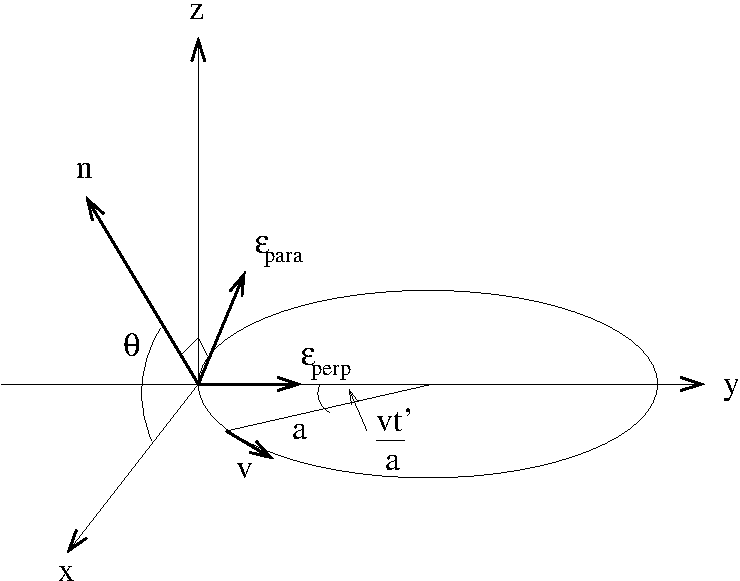
\includegraphics[width=\textwidth]{syncfig}
}
\caption{Geometry of synchrotron emission}
\end{figure}
}

With no loss of generality we can assume that the particle gyrates in
the $x - y -$plane and our line of sight is in the $x - z -$plane and
makes an angle with the $x-$axis. With this geometric setup we can
calculate 
\begin{equation}
{\bf n} \times ({\bf n} \times \betabold) = -\epbold_\perp \sin \left
( \frac{v t'}{a} \right ) + \epbold_\| \cos \left ( \frac{v t'}{a} \right )
\sin \theta
\label{eq:384}
\end{equation}
The term in the exponential is the observed time in terms of the
retarded time, 
\begin{eqnarray}
t' - \frac{{\bf n} \cdot {\bf r}(t')}{c} &=& t' - \frac{a}{c} \cos
\theta
\sin \left ( \frac{v t'}{a} \right ) \\
&\approx& t' - \frac{a}{c} \left ( 1 - \frac{\theta^2}{2} \right )
\left [ \frac{v t'}{a} - \frac{1}{6} \left ( \frac{v t'}{a} \right )^3
\right ] \\
&\approx& t' - \beta t' + \frac{\theta^2}{2} \beta t' + \frac{c^2
\beta^3 t'^3}{6 a^2} \\
&\approx& \left ( 2 \gamma^2 \right )^{-1} \left [ \left ( 1 +
\gamma^2 \theta^2 \right ) t' + \frac{c^2 \gamma^2 t'^3}{3a^2} \right ]
\label{eq:385}
\end{eqnarray}
To get the final equation we took $1 - \beta \rightarrow
(2\gamma)^{-1}$
and $\beta \rightarrow 1$
.
   Substituting these results into equation (25) and taking the small-angle
approximation for the polarization vectors as well yield
\begin{eqnarray}
\dd{W}{\omega d\Omega} &\equiv& \dd{W_\|}{\omega d\Omega} 
+ \dd{W_\perp}{\omega d\Omega} \\
\dd{W_\perp}{\omega d\Omega} &=& 
\frac{q^2 \omega^2}{4\pi^2 c} \left | 
\int \frac{ct'}{a} \exp \left [ \frac{i\omega}{2\gamma^2} \left (
\theta^2_\gamma t' + \frac{c^2 \gamma^2 t'^3}{3a^2} \right ) \right ]
dt' \right |^2\\
\dd{W_\|}{\omega d\Omega} &=& 
\frac{q^2 \omega^2 \theta^2}{4\pi^2 c} \left | 
\int \exp \left [ \frac{i\omega}{2\gamma^2} \left (
\theta^2_\gamma t' + \frac{c^2 \gamma^2 t'^3}{3a^2} \right ) \right ]
dt' \right |^2
\label{eq:386}
\end{eqnarray}
where $\theta_\gamma^2=1 + \gamma^2 \theta^2$.

Let's make the following change of variables,
\begin{equation}
y \equiv \gamma \frac{c t'}{a \theta_\gamma} ~\rmmat{and}~ \eta \equiv
\frac{\omega a \theta_\gamma^3}{3 c \gamma^3} \approx \frac{\omega}{2\omega_c}
\label{eq:387}
\end{equation}
to yield
\begin{eqnarray}
\dd{W_\perp}{\omega d\Omega} &=& 
\frac{q^2 \omega^2}{4\pi^2 c} 
\left ( \frac{a \theta^2_\gamma}{\gamma^2 c} \right )^2
\left | 
\int_{-\infty}^\infty y \exp \left [ \frac{3}{2} i \eta \left ( y +
\frac{1}{3} y^3 \right ) \right ]
dt' \right |^2\\
\dd{W_\|}{\omega d\Omega} &=& 
\frac{q^2 \omega^2 \theta^2}{4\pi^2 c} 
\left ( \frac{a \theta_\gamma}{\gamma c} \right )^2
\left | 
\int_{-\infty}^\infty y \exp \left [ \frac{3}{2} i \eta \left ( y +
\frac{1}{3} y^3 \right ) \right ]
dt' \right |^2\\
\label{eq:388}
\end{eqnarray}

% \begin{figure}
% \begin{center}
% 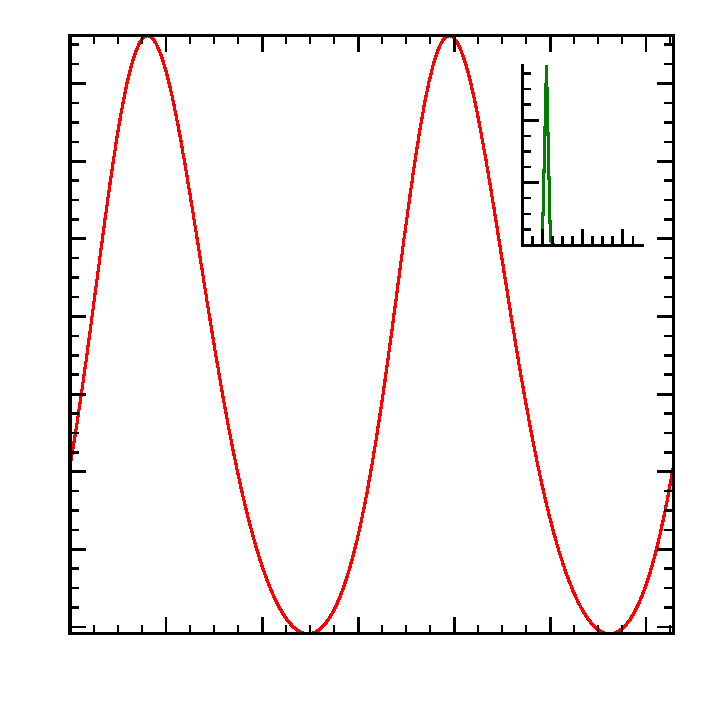
\includegraphics[width=0.49\columnwidth]{syncct_1}
% 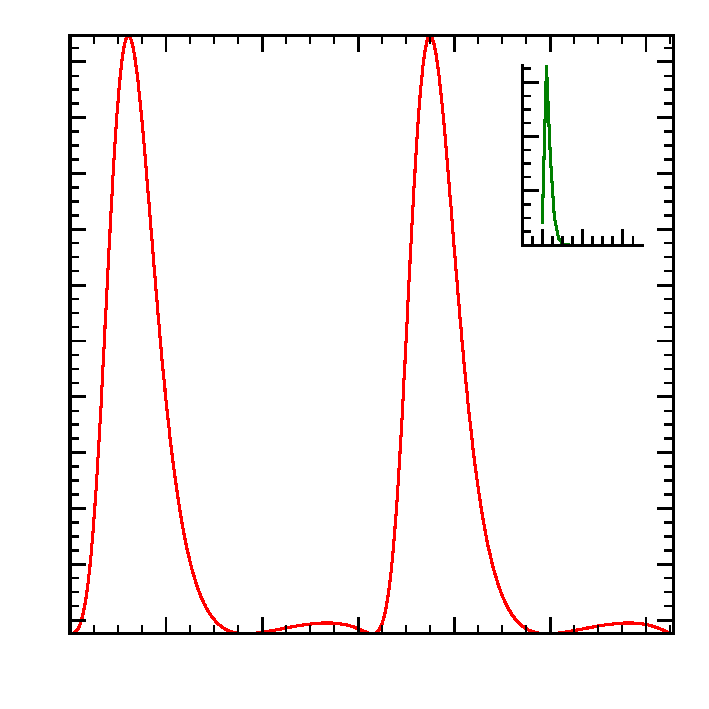
\includegraphics[width=0.49\columnwidth]{syncct_5} 

% 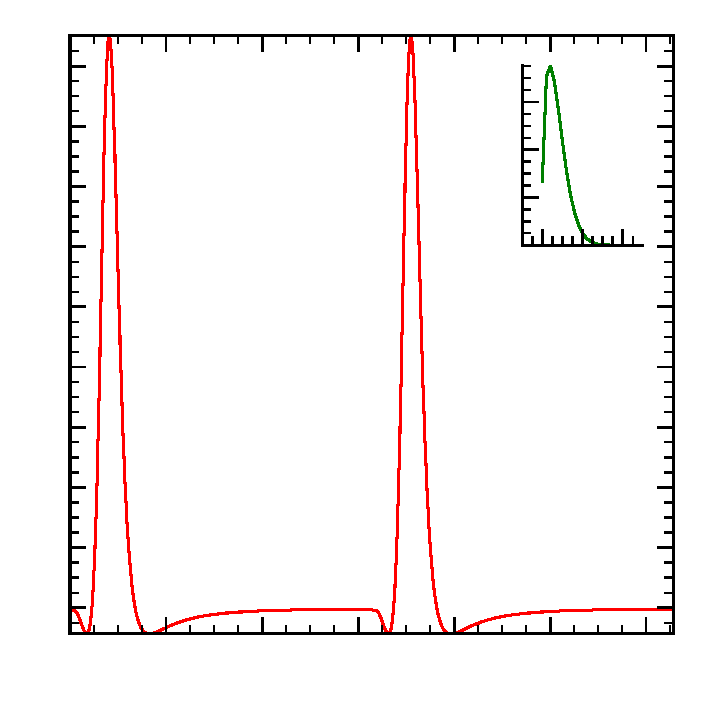
\includegraphics[width=0.49\columnwidth]{syncct_9}
% 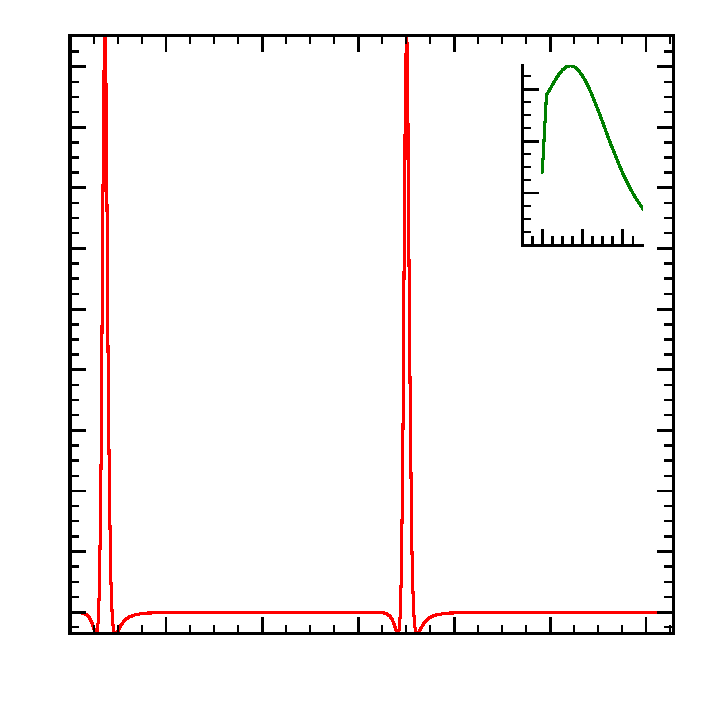
\includegraphics[width=0.49\columnwidth]{syncct_99} 
% \end{center}
% \caption{Electric field from a gyrating particle
%  $\beta = 0.1, 0.5, 0.9$ and 0.99.  The insets show the power spectrum
% with $\omega/\omega_c$ along the $x-$axis.  These were calculated
% without the small-angle or ultrarelativistic approximations.  Keep in
% mind a particle with $\gamma=10^3$ has $\beta=0.9999995$.
% }
% \end{figure}

\begin{figure}
\begin{center}
\begin{tikzpicture}
\begin{scope}[yscale=2,xscale=0.4]
\draw plot file{sync/syncmin_0.1} (-3.2,0.6) node {$\beta=0.1$};
\pgftransformxshift{400}
\draw plot file{sync/syncmin_0.5} (-3.6,0.4) node {$\beta=0.5$};
\pgftransformyshift{-40}
\draw plot file{sync/syncmin_0.99} (-4,0.4) node {$\beta=0.99$};
\pgftransformxshift{-400}
\draw plot file{sync/syncmin_0.9} (-4,0.4) node {$\beta=0.9$};
\end{scope}
\begin{scope}[xscale=0.07]
\pgftransformxshift{180}
\pgftransformyshift{25}
\draw plot [yscale=4] file{sync/psync_0.1} ;
\pgftransformxshift{2200}
\draw plot [yscale=20] file{sync/psync_0.5} ;
\pgftransformyshift{-80}
\draw plot [yscale=1000] file{sync/psync_0.99} ;
\pgftransformxshift{-2200}
\draw plot [yscale=100] file{sync/psync_0.9} ;
\end{scope}
\draw [->] (-3.7,-3.2) -- (8,-3.2) node [right] {$t$};
\draw [->] (-3.5,-3.4) -- (-3.5,2) node [above] {$E(t)$};
\end{tikzpicture}
\end{center}
\caption{Electric field from a gyrating particle
 $\beta = 0.1, 0.5, 0.9$ and 0.99.  The insets show the power spectrum
with $\omega/\omega_c$ along the $x-$axis.  These were calculated
without the small-angle or ultrarelativistic approximations.  Keep in
mind a particle with $\gamma=10^3$ has $\beta=0.9999995$.
}
\end{figure}

It turns out that these integrals can be performed with some special
functions called Airy integrals or modified Bessel functions to yield,
\begin{eqnarray}
\dd{W_\perp}{\omega d\Omega} &=& 
\frac{q^2 \omega^2}{4\pi^2 c} 
\left ( \frac{a \theta^2_\gamma}{\gamma^2 c} \right )^2
K^2_\frac{2}{3} (\eta)\\
\dd{W_\|}{\omega d\Omega} &=& 
\frac{q^2 \omega^2 \theta^2}{4\pi^2 c} 
\left ( \frac{a \theta_\gamma}{\gamma c} \right )^2
K^2_\frac{1}{3} (\eta)
\label{eq:389}
\end{eqnarray}

    We would like to find the total emission per orbit over all solid angles.
The emission lies within an angle $1/\gamma$ 
of a cone of half-angle $\alpha$ centered on
the magnetic field, so we can take the element of solid angle 
$d\Omega = 2 \sin \alpha d \theta$
and integrate,
\begin{eqnarray}
\dd{W_\perp}{\omega} &=& 
\frac{2 q^2 \omega^2 a^2 \sin\alpha}{3\pi c^3 \gamma^4}
\int_{-\infty}^\infty
\theta_\gamma^4
K^2_\frac{2}{3} (\eta)
d\theta 
\\
\dd{W_\|}{\omega} &=& 
\frac{2 q^2 \omega^2 a^2 \sin\alpha}{3\pi c^3 \gamma^4}
\int_{-\infty}^\infty
\theta_\gamma^2 \theta^2
K^2_\frac{1}{3} (\eta)
d\theta 
\label{eq:390}
\end{eqnarray}

These integrals can be written in terms of Bessel functions to yield,
\begin{eqnarray}
\dd{W_\perp}{\omega} &=& 
\frac{\sqrt{3} q^2 \gamma \sin\alpha}{2c} \left [ F(x) + G(x) \right ]
\\
\dd{W_\|}{\omega} &=& 
\frac{\sqrt{3} q^2 \gamma \sin\alpha}{2c} \left [ F(x) - G(x) \right ]
\label{eq:391}
\end{eqnarray}
where
\begin{equation}
F(x) = x \int_x^\infty K_\frac{5}{3}(\xi) d\xi, 
~~~~~~~
G(x) = x K_\frac{2}{3}(x)
\label{eq:392}
\end{equation}
and x = $\omega/\omega_c$ .
% \begin{figure}
% \begin{center}
% \begin{tikzpicture}
% \begin{scope}[yscale=3,xscale=2,smooth]
% \draw[very thin,color=gray] (-0.02,-0.02) grid [ystep=0.5] (5.1,1.1);
% \draw[->] (-0.2,0) -- (5.2,0) node[right] {$x$}; 
% \draw[->] (0,-0.2) -- (0,1.2) node[above] {$F(x),G(x)$};
% \draw (0.72,0.9) node {$F(x)$} (1.5,0.25) node {$G(x)$};
% \draw (0,1) node [left] {\small 1};
% \draw (0,0.5) node [left] {\small 0.5};
% \foreach \x in {1,...,5} 
%   \draw (\x,0) node [below] {\small \x};
% \draw[color=red] plot  file{sync/syncf.dat};
% \draw[color=blue] plot file{sync/syncg.dat};
% \end{scope}
% \end{tikzpicture}
% \end{center}
% \caption{Synchrotron Functions}
% \label{fig:fgfunk}
% \end{figure}
\begin{figure}
\begin{center}
\begin{tikzpicture}
\begin{scope}[scale=2.5,smooth]
\clip (-2.5,-3) rectangle (1,2) ;
\draw[color=red] plot file{sync/lsyncf.dat} ;
\draw[color=blue] plot file{sync/lsyncg.dat};
\end{scope}
\begin{scope}[scale=2.5]
\draw[very thin,color=gray] (-2.52,-3.02) grid [ystep=1] (0.7,-0.8);
\draw[->] (-2.7,-3) -- (0.7,-3) node[right] {$x$}; 
\draw[->] (-2.5,-3.2) -- (-2.5,-0.8) node[above] {$F(x),G(x)$};
\draw (-1.8,-1.3) node {$F(x)$} (-1.8,-1.9) node {$G(x)$};
\foreach \x in {-2,...,0} 
  \draw (\x,-3) node [below] {\small $10^{\x}$};
\foreach \x in {-2,...,-1} 
  \draw (-2.5,\x) node [left] {\small $10^{\x}$};
\end{scope}
\end{tikzpicture}
\end{center}
\caption{Synchrotron Functions}
\label{fig:lfgfunk}
\end{figure}

{\bf Something to think about.} Why could we take the limits of integration
in equations (35) and (36) and (39) and (40) to be infinite?

    To convert these values in a power per frequency we have to divide by
the orbital period of the charge $T = 2\pi /\omega_B$ to give
\begin{eqnarray}
P_\perp &=& 
\frac{\sqrt{3} q^3 B \sin\alpha}{4\pi m c^2} \left [ F(x) + G(x) \right ]
\\
P_\| &=& 
\frac{\sqrt{3} q^3 B \sin\alpha}{4\pi m c^2} \left [ F(x) - G(x) \right ]
\label{eq:393}
\end{eqnarray}
The total power is proportional to $F(x)$ that has the following asymptotic
values,
\begin{eqnarray}
F(x) &\sim& \frac{4\pi}{\sqrt{3} \Gamma \left ( \frac{1}{3} \right )}
\left ( \frac{x}{2} \right )^{1/3}, ~~ x \ll\ 1
\label{eq:835} \\
F(x) &\sim& \left(\frac{\pi}{2}\right)^{1/2} e^{-x} x^{1/2}
, ~~ x \gg\ 1 
\label{eq:394}
\end{eqnarray}


\section{Synchrotron Absorption}
\label{sec:synchr-absorpt}

We are particularly interested in the form of the spectrum from a
power-law distribution of particles for frequencies where the region
is optically thick.  We know from the formal soltuion of radiative
transfer that the spectrum approaches the source function at large
optical depth.  Furthermore Eq.~\ref{eq:78} yields a relationship
between the number of particles of various energies and the volume of
phase space at each energy
\begin{equation}
S_\nu = \frac{2h\nu^3}{c^2} \left (
\frac{g_2 n_1}{g_1 n_2} - 1 \right )^{-1}.
\label{eq:838}
\end{equation}
For free ultrarelativistic particles the density of states is
proportional to $E^2$, and we have assumed that their number is
proportional to $E^{-p}$.   Let us imagine that synchrotron emission
is a transition between the upper state at an energy $E+h\nu$ and the
lower state at energy $E$, so
\begin{equation}
\frac{g_2 n_1}{g_1 n_2} - 1 = \frac{(E+h\nu)^2 E^{-p}}{E^2
  (E+h\nu)^{-p}} - 1 = \left ( 1 + \frac{h\nu}{E}\right )^{p+2} - 1
\approx \left ( p + 2 \right ) \frac{h \nu}{E}
\label{eq:840}
\end{equation}
where the final result obtains in the classical limit where $h\nu \ll
E$, so we have
\begin{equation}
S_\nu \approx \frac{2h\nu^3}{c^2} \frac{E}{\left (p+2\right) h \nu}
\approx \frac{2}{\left (p+2\right)} \left ( \frac{4\pi}{3}
  \frac{m^3 c}{q B \sin\alpha} \right )^{1/2} \nu^{5/2}
\label{eq:841}
\end{equation}
where we have related the energy of the state ($E$) to the frequency
through Eq.~\ref{eq:371}.  Notice that the spectral index does not
depend on the power-law index of the particle distribution but rather
results from the power-law relationship between particle energy and
frequency.  Because the optically thin emission spectrum increases
more slowly with frequency than the source function (or even
decreases), we expect synchrotron absorption to be important at low
frequencies where the the integrated optically thin emission exceeds
the source function.


\section{A Complete Synchrotron Spectrum}
 \label{sec:compl-synchr-spectr}
The complete spectrum from synchrotron radiation must account for the
evolution of the electron energies, absorption, the minimum electron
energy and the age of the source.  We have all the necessary
ingredients to figure this out.  First,
\S~\ref{sec:spectral-index-power} calculates the shape of the photon
spectrum for a given power-law distribution of electron energies.
The second ingredient is to calculate the distribution of electron
energies as a function of the time since the electrons were
accelerated (or {\em injected}).   Let us assume that the electrons
initially have a power-law distribution of energies
\begin{equation}
\dd{N}{t d\gamma_0} = C \gamma_0^{-p}  ~\mathrm{for}~\gamma_0>\gamma_m.
\end{equation}
Furthermore the electron energies decrease with time according to
\begin{equation}
\gamma = \frac{\gamma_0 }{1 + A \gamma_0 t'} , A = \frac{2 q^4
  B_\perp^2}{3m^3 c^5}
\label{eq:836}
\end{equation}
where $t'$ is the time since the particles were accelerated
By inverting this equation we obtain the initial electron energy in terms
of the final electron energy
\begin{equation}
  \gamma_0 = \frac{\gamma}{1-A\gamma t'} 
\end{equation}
and
\begin{equation}
   \dd{\gamma_0}{\gamma} = \frac{1}{\left( 1- A \gamma t' \right)^2}
\end{equation}
so
\begin{equation}
\dd{N}{\gamma d t} = C \gamma^{-p} \left ( 1 - A \gamma t' \right )^{p-2}.
\end{equation}
It is crucial to understand the validity of this distribution. Clearly
we must have 
\begin{equation}
\frac{\gamma_m}{1+A\gamma_m t'} < \gamma <
\frac{1}{At'}.
\label{eq:830}
\end{equation}
Otherwise the number of electrons vanishes because either they have
not yet had time to cool to such a low energy or they have already
cooled below this energy.  The original power-law distribution is
truncated at high energies and is extended below $\gamma_m$
by cooling.  

If the source were only active instantaneously or for a short time
long ago $\Delta t \ll t'$, this would be sufficient, but if we are
interested in a source that has been active continually from some time
ago we must intergrate this distribution over the injection times in
the past.  The resulting distribution is 
\begin{equation}
  \dd{N}{\gamma} = C \gamma^{-p} \int_{t_0}^{t_1} \left( 1 - A
  \gamma t'\right )^{p-2} d t' =C \gamma^{-p} \left . \frac{(1 - A
  \gamma t')^{p-1}}{(p-1) (-A\gamma)} \right |_{t_0}^{t_1}
\end{equation}
where the conditions in Eq.~\ref{eq:830} determine the values of $t_0$
and $t_1$.  We have
\begin{equation}
  t_0 = \max\left [0, \frac{1}{A} \left (\gamma^{-1} -
      \gamma_m^{-1} \right ) \right ]~\mathrm{and}~t_1=\min
  \left (t, \frac{1}{A\gamma} \right ).
\label{eq:831}
\end{equation}
The latter expression in Eq.~\ref{eq:831} encourages us to define
\begin{equation}
\gamma_c = \frac{1}{At}.
\end{equation}
We will use this quantity to eliminate $A$ from the equations.
The energy divides the electrons into those that have had a chance to
cool significantly since the source turned on a time $t$ ago and those
that have not cooled significantly.   There are two possibilities for
the resulting distribution depending on whether $\gamma_c$
exceeds $\gamma_m$.  We will examine the distribution for
$\gamma_c>\gamma_m$ first; this is known as the
{\em slow cooling} regime.  There are three possibly ranges for
$\gamma$.  First at the highest energies we have 
\begin{equation}
\dd{N}{\gamma} = \frac{Ct \gamma_c}{p-1} \gamma^{-(p+1)}~\mathrm{for}~\gamma_m< \gamma_c <\gamma.
\label{eq:832}
\end{equation}
For intermediate energies we have
\begin{equation}
\dd{N}{\gamma} = \frac{Ct \gamma_c}{p-1} \gamma^{-(p+1)} \left [ 1 - \left ( 1 - \frac{\gamma}{\gamma_c}
    \right)^{p-1} \right ] ~\mathrm{for}~\gamma_m < \gamma<  \gamma_c 
\label{eq:833}
\end{equation}
For $\gamma \ll\ \gamma_c$ this reduces to
\begin{equation}
\dd{N}{\gamma} \approx  C t \gamma^{-p} ~\mathrm{for}~  \gamma_m < \gamma \ll \gamma_c .
\label{eq:833}
\end{equation}
For the lowest energies the following expression obtains
\begin{equation}
\dd{N}{\gamma} = 
\frac{C t \gamma_c}{p-1} \gamma^{-(p+1)} \left [ \left (\frac{\gamma}{\gamma_m} \right
  )^{p-1} - \left ( 1 - \frac{\gamma}{\gamma_c} \right)^{p-1} \right ]
 ~\mathrm{for}~  \gamma < \gamma_m <  \gamma_c .
\label{eq:834}
\end{equation}

The other cooling regmine is called {\em fast cooling} where
$\gamma_c < \gamma_m$.  Is this regime for the
largest energies $\gamma>\gamma_m>\gamma_c$,
Eq.~\ref{eq:832} also holds.   For intermediate energies we have
\begin{equation}
\dd{N}{\gamma} = \frac{Ct \gamma_c}{(p-1) \gamma_m^{p-1}} \gamma^{-2}~\mathrm{for}~\gamma_c<\gamma<\gamma_m.
\end{equation}
and for the smallest energies
$\gamma<\gamma_c<\gamma_m$ Eq.~\ref{eq:834}
again obtains.

Both of the distributions either for slow or fast cooling vanish for
\begin{equation}
  \gamma < \gamma_\mathrm{cut-off} = \left (
    \frac{1}{\gamma_m} +\frac{1}{\gamma_c}
  \right )^{-1}.
\end{equation}
Well into the slow cooling regime we have $\gamma_m\ll
\gamma_c$ so $\gamma_\mathrm{cut-off} \approx
\gamma_m$.  Well into the fast cooling regime we have
$\gamma_\mathrm{cut-off} \approx \gamma_c$.  To find the
distribution of photon energies we have to convolve the electron
distribution with the function $F(x)$.  
For $\omega > \omega_\mathrm{max}$ where
\begin{equation}
\omega_\mathrm{max} = \frac{3 \gamma_\mathrm{cut-off}^2 q B \sin
  \alpha}{2mc}
\end{equation}
the results of \S~\ref{sec:spectral-index-power} apply.  On the other
hand below this frequency, the radiation results from the
low-frequency limit of the function $F(x)$ (Eq.~\ref{eq:835}),
i.e. $F_\omega \propto \omega^{1/3}$.   A second complication is the
role of synchrotron absorption outlined in
\S~\ref{sec:synchr-absorpt}.   We can combine the various results from
this section to derive a schematic of the emission spectrum from a
synchrotron cooling population of electrons with constant particle
injection.   Figs.~\ref{fig:sync_slow}
and~\ref{fig:sync_fast} depict the spectrum for slow and fast cooling.

% \begin{table}
% \caption{Regimes of Synchrotron Cooling}
% \label{tab:synch-cool}
% \begin{center}
% \begin{tabular}{cccc}
% \hline
% \hline
% Lorentz Factor Range & $dN/d\gamma$ & Frequency Range & $F_\omega$ \\
% \hline
% \multicolumn{4}{c}{\em slow cooling} \\
% \hline
% $\gamma>\gamma_c = \frac{3 m^3 c^5}{2 q^4 B_\perp^2 t}$ &
% $\gamma^{-(p+1)}$ & $\omega > \omega_c=\frac{27}{8} \frac{m^5
%   c^9}{q^7 B_\perp^3 t^2}$ & $F_{\omega,m} \frac{\omega_m^{(p-1)/2} \omega_c^{1/2}}{\omega^{p/2}}$
%  \\
% $\gamma_m < \gamma < \gamma_c$ & \gamma^{-p} & $\omega_m < \omega <
% \omega_c$ & $F_m \left ( \frac{\omega_m}{\omega} \right )^{-(p-1)/2}$ \\
% ? ? & ? & ? ? & ? \\
% ? ? & ? & ? ? & ? \\
% \hline
% \multicolumn{4}{c}{\em fast cooling} \\
% \hline
% ? ? & ? & ? ? & ? \\
% ? ? & ? & ? ? & ? \\
% ? ? & ? & ? ? & ? \\
% ? ? & ? & ? ? & ? \\
% \hline
% \end{tabular}
% \end{center}
% \end{table}

\begin{figure}
\begin{center}
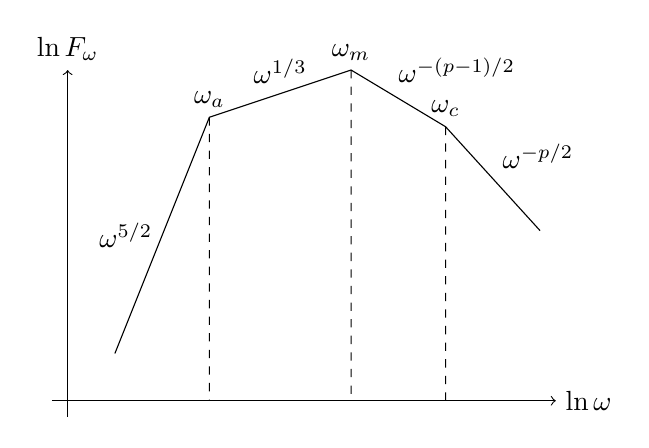
\begin{tikzpicture}
\draw[->] (-0.2,0) -- (6.2,0) node[right] {$\ln \omega$}; 
\draw[->] (0,-0.2) -- (0,4.2) node[above] {$\ln F_\omega$};
\begin{scope}[scale=6]
\draw  (0.1,0.1) -- 
  ++(0.2,0.5) node [above] (oma) {$\omega_a$} 
  node [pos=0.5,left] {$\omega^{5/2}$} -- 
++(0.3,0.1) node [above] (ommi) {$\omega_m$} 
  node [pos=0.5,above] {$\omega^{1/3}$} --
++(0.2,-0.12) node [above] (omc) {$\omega_c$} 
node [pos=0.4,above right] {$\omega^{-(p-1)/2}$} -- 
++(0.2,-0.22) node [pos=0.5,above right] {$\omega^{-p/2}$} ;
\draw [dashed] (oma) -- (0.3,0) (ommi) -- (0.6,0) (omc) -- (0.8,0);
\end{scope}
\end{tikzpicture}
\end{center}
\caption{Complete synchrotron spectrum for an age less than the
  maximum cooling time (slow cooling).}
\label{fig:sync_slow}
\end{figure}

\begin{figure}
\begin{center}
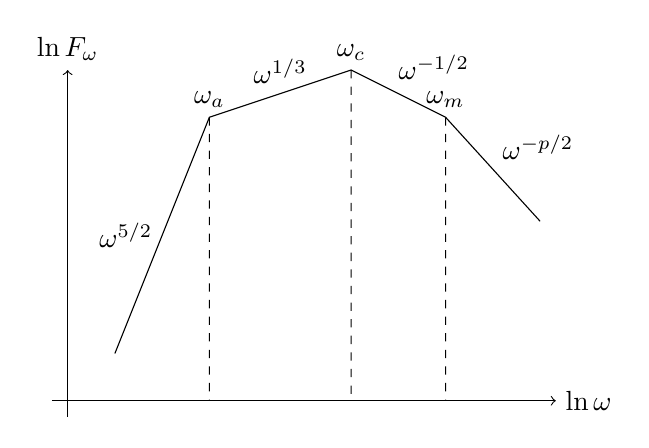
\begin{tikzpicture}
\draw[->] (-0.2,0) -- (6.2,0) node[right] {$\ln \omega$}; 
\draw[->] (0,-0.2) -- (0,4.2) node[above] {$\ln F_\omega$};
\begin{scope}[scale=6]
\draw  (0.1,0.1) -- 
  ++(0.2,0.5) node [above] (oma) {$\omega_a$} 
  node [pos=0.5,left] {$\omega^{5/2}$} -- 
++(0.3,0.1) node [above] (omc) {$\omega_c$} 
  node [pos=0.5,above] {$\omega^{1/3}$} --
++(0.2,-0.1) node [above] (ommi) {$\omega_m$} 
node [pos=0.4,above right] {$\omega^{-1/2}$} -- 
++(0.2,-0.22) node [pos=0.5,above right] {$\omega^{-p/2}$} ;
\draw [dashed] (oma) -- (0.3,0) (omc) -- (0.6,0) (ommi) -- (0.8,0);
\end{scope}
\end{tikzpicture}
\end{center}
\caption{Complete synchrotron spectrum for an age greater than the
  maximum cooling time (fast cooling).}
\label{fig:sync_fast}
\end{figure}

To learn more about the frequency spectrum of synchrotron emission
from mono-energetic electrons, consult Chapter \S14.6
of
\begin{itemize}
\item Jackson, J. D., {\em Classical Electrodynamics}.
\end{itemize}

\section{Problems}
\begin{enumerate}
\item{\bf Synchrotron Radiation:}

An ultrarelativistic electron emits synchrotron radiation.  Show that
its energy decreases with time according to
\begin{equation}
\gamma = \gamma_0 \left ( 1 + A \gamma_0 t \right )^{-1}, A=\frac{2e^4
  B_\perp^2}{3m^3 c^5}.
\label{eq:395}
\end{equation}
Here $\gamma_0$ is the initial value of $\gamma$ and $B_\perp = B
\sin\alpha$.  Show that the time for the electron to lose half its
energy is
\begin{equation}
t_{1/2} = \left (A\gamma_0\right)^{-1}
\label{eq:396}
\end{equation}
How do you reconcile the decrease of $\gamma$ with the result of
constant $\gamma$ for motion in a magnetic field?

\item{\bf Synchrotron Cooling More Precisely:}

Derive the evolution of the energy of the electron (or $\gamma$)
evolves in time without making the ultrarelativistic approximation.

\item{\bf Power-Law Distribution More Precisely:}

Calculate the photon spectrum for a power-law distribution of electron
energies as in \S~\ref{sec:spectral-index-power} including the
normalization and polarization. 

\end{enumerate}
%%% Local Variables:
%%% TeX-master: "book"
%%% End:

\chapter{Compton Scattering}
\label{cha:compton-scattering}\index{Compton scattering}
When we looked at the scattering of light by electrons we assumed that
the energy of photon was not changed by the scattering and that the
electron was not relativistic.  Compton scattering involves dropping
these two assumptions.

\section{The Kinematics of Photon Scattering}
\label{sec:kinem-phot-scatt}
\index{Compton scattering!kinematics}

We assumed that the light carries only energy but it also carries
momentum so when an electron scatters light some momentum may be
transferred between the light and the electron.  Let's consider that
the electron is at rest (we can always move into the frame of the
electron).  Initially we have
\begin{equation}
p^\mu_{ei} = \left [ \begin{array}{c}mc\\ {\bf 0}  \end{array} \right
] ~\rmmat{and}~ p^\mu_{\gamma i} = \frac{E_i}{c} \left [
  \begin{array}{c}1 \\ {\bf n}_i  \end{array} \right
]
\label{eq:397}
\end{equation}
and after the scattering we have
\begin{equation}
p^\mu_{ef} = \left [ \begin{array}{c}\frac{E}{c}\\ {\bf p}  \end{array} \right
] ~\rmmat{and}~ p^\mu_{\gamma i} = \frac{E_f}{c} \left [
  \begin{array}{c}1 \\ {\bf n}_f  \end{array} \right
]
\label{eq:398}
\end{equation}
The conservation of energy-momentum tells us that
\begin{equation}
p^\mu_{ei} + p^\mu_{\gamma i}  = p^\mu_{ef} + p^\mu_{\gamma f} 
\label{eq:399}
\end{equation}
or
\begin{equation}
p^\mu_{ef}  = p^\mu_{ei} + p^\mu_{\gamma i} -  p^\mu_{\gamma f} 
\label{eq:400}
\end{equation}
Let's calculate the square of both sides,
\begin{eqnarray}
p^\mu_{ef} 
p_{\mu,ef} &=&
( p^\mu_{ei} + p^\mu_{\gamma i} -  p^\mu_{\gamma f} ) 
( p_{\mu,ei} + p_{\mu,\gamma i} -  p_{\mu,\gamma f} ) \\
m^2 c^2 &=& m^2 c^2 + 2 p^\mu_{ei} p_{\mu,\gamma i} - 2p^\mu_{ei}
p_{\mu,\gamma f} - 2 p^\mu_{\gamma f} p_{\mu,\gamma i}  \\
0 &=& 2 m E_i - 2 m E_f - 2 \frac{E_i E_f}{c^2} \left ( 1 - \cos\theta
\right ) \\
E_f &=& \frac{E_i}{1+ \frac{E_i}{mc^2} \left ( 1 - \cos\theta
\right )}
\label{eq:401}
\end{eqnarray}
We can write this really compactly by using the relationship between
the energy and wavelength of a photon ($E=hc/\lambda$),
\begin{equation}
\lambda_f = \lambda_i + \frac{h}{mc} \left (1 - \cos \theta \right )
\label{eq:402}
\end{equation}
A cute thing to ask is what is the final energy of the photon if the 
initial energy is much greater than the electron's rest-mass.  We get
\begin{equation}
E_f \approx \frac{mc^2}{1-\cos\theta}
\label{eq:403}
\end{equation}

There is a second important change.  If the energy of the photon
changes dramatically, {\em i.e.} $E_f \ll E_i$, the cross section for
the scattering is reduced from $\sigma_T$. Specifically
\begin{equation}
\dd{\sigma}{\Omega} = \frac{r_0^2}{2} \left ( \frac{E_f}{E_i}
\right )^2 \left ( \frac{E_i}{E_f} + \frac{E_f}{E_i} - \sin^2 \theta
\right )
\label{eq:404}
\end{equation}
for unpolarized radiation. 

\section{Inverse Compton Scattering}
\label{sec:inverse-compt-scatt}
\index{inverse Compton scattering}
\index{Compton scattering!inverse}

In Compton scattering the photon always loses energy to an electron
initially at rest.   Inverse Compton scattering corresponds to the
situation where the photon gains energy from the electron because the
electron is in motion.

Let's imagine that the electron is travelling along the $x-$axis with
Lorentz factor $\gamma$.  Furthermore, let's think about the lab frame
(unprimed) and the electron's rest frame (primed).  The initial and
final energies 
\begin{equation}
E_i' = E_i \gamma \left ( 1 - \beta \cos \theta_i \right )~\rmmat{and}~
E_f = E_f' \gamma \left ( 1 - \beta \cos \theta_f' \right )
\label{eq:405}
\end{equation}
where $\theta$ is the angle that the photon makes with the $x-$axis in
the lab frame.  Furthermore, we know that
\begin{equation}
E'_f = \frac{E'_i}{1+ \frac{E'_i}{mc^2} \left ( 1 - \cos\Theta \right)}
\label{eq:406}
\end{equation}
where $\Theta$ is the angle between the incident and scattered photon
in the rest-frame of the electron.

Let's consider the case we $E_i' \ll m c^2$ so $E_i' \approx E_f'$.
If we look at the redshift formulae we find that
\begin{equation}
E_f = E_i \gamma^2 \left ( 1 - \beta \cos \theta \right ) \left ( 1 +
\beta \cos \theta_f' \right )
\label{eq:407}
\end{equation}
Let's consider the case of relativistic electrons.  If we assume that
the photon distribution is isotropic, the angle $\langle \cos\theta
\rangle = 0$.  $\langle \cos\theta_f'\rangle$ is also zero because the
scatter photon is forward-backward symmetric in the rest-frame of the
electron so we
find that
\begin{equation}
E_f = \gamma^2 E_i
\label{eq:408}
\end{equation}
when averaged over angle.

\subsection{Inverse Compton Power - Single Scattering}
\label{sec:inverse-compt-power}

Let's consider an isotropic distribution of photons and
derive the total power emitted by an electron passing through. 

We will first make use on some of the transformation rules that we
derived for the phase-space density of photons.  Let $v dE$ be the
density of photons having energy in the range $dE$.  The number of
photons in a box over the energy range is a Lorentz invariant
\begin{equation}
v dE d^3 x = v' dE' d^3 x'
\label{eq:409}
\end{equation}
Remember that $d^3 x = \gamma^{-1} d^3 x'$ and that $E = \gamma E'$ (with
forward-backward symmetry) so we
find that
\begin{equation}
\frac{v dE}{E} = \frac{v' dE'}{E'} = \rmmat{Lorentz Invariant}
\label{eq:410}
\end{equation}
Let's switch to the rest-frame of the electron.   The total power
scattered in the electron's rest frame is
\begin{equation}
\dd{E_f}{t} = \dd{E_f'}{t'} = c \sigma_T \int E_f' v' d E'
\label{eq:411}
\end{equation}
where we have assumed that $E_i' \ll m c^2$.  The first equality holds
because the emitted power is a Lorentz invariant. {\bf Why is this true?}

Let's assume that the change in the energy of the photon in the
rest frame of the electron is negligible compared to the change in the
energy of the photon in the lab frame, {\em i.e.} $\gamma^2 - 1 \gg
E/(m c^2)$, so $E_f'=E'$, so we have
\begin{equation}
\dd{E_f}{t} = c \sigma_T \int E'^2 \frac{v' dE'}{E'} = c
\sigma_T \int E'^2 \frac{v dE}{E}
\label{eq:412}
\end{equation}
The redshift formula for photons is 
\begin{equation}
E' = E \gamma \left ( 1 - \beta \cos\theta \right )
\label{eq:413}
\end{equation}
so we have
\begin{equation}
\dd{E_f}{t} = c \sigma_T \gamma^2 \int \left ( 1  - \beta
\cos\theta \right )^2 E v dE = c \sigma_T \gamma^2 \left ( 1 + \frac{1}{3}
\beta^2 \right ) U_\rmscr{ph}
\label{eq:414}
\end{equation}
where
\begin{equation}
U_\rmscr{ph} = \int E v dE
\label{eq:415}
\end{equation}

The rate of decrease of the total initial photon energy is
\begin{equation}
\dd{E}{t} = -c\sigma_T \int E v dE = -\sigma_T c U_\rmscr{ph}
\label{eq:416}
\end{equation}
so the total change in the energy of the electron and converted into
the increased energy of the radiation field is
\begin{equation}
\dd{E_\rmscr{rad}}{t} = \dd{E_f}{t} + \dd{E}{t} = c\sigma_T
U_\rmscr{ph} \left [ \gamma^2 \left ( 1 + \frac{1}{3} \beta^2 \right )
  - 1 \right ] = \frac{4}{3} \sigma_T c \gamma^2 \beta^2 U_\rmscr{ph}.
\label{eq:417}
\end{equation}
Let's compare this with the synchrotron power of the same electron,
\begin{equation}
P = 
\frac{2}{3} r_0^2 c \beta^2_\perp \gamma^2 B^2 = \frac{2}{3}
\left ( \frac{3}{8\pi} \sigma_T \right ) c \left ( \frac{2}{3} \beta^2
\right ) \left ( 8\pi U_B \right ) = \frac{4}{3} \sigma_T c \gamma^2 \beta^2
 U_B 
\label{eq:418}
\end{equation}
\subsection{Inverse Compton Spectra - Single Scattering}
\label{sec:inverse-compt-spectr}

Let's suppose that we have an isotropic distribution of photons of a
single energy $E_0$ and a beam of electrons travelling along the
$x-$axis with energy $\gamma m c^2$ and density $N$.  Let's also use
an intensity that counts the number of photons not their energies so
\begin{equation}
I(E) = \frac{I_\nu}{h \nu} = F_0 \delta (E-E_0).
\label{eq:419}
\end{equation}
What does the intensity look like in the rest frame of the electrons.
Remember that $I_\nu/\nu^3$ was a Lorentz invariant so we have
\begin{eqnarray}
I'(E',\mu') &=& F_0 \left (\frac{E'}{E}\right)^2 \delta (E-E_0)\\
& =& F_0
\left (\frac{E'}{E_0}\right)^2 \delta (\gamma E' (1+\beta\mu') -E_0) \\
&=&  \frac{F_0}{\gamma\beta E'} 
\left (\frac{E'}{E_0}\right)^2 \delta \left (\mu' - \frac{E_0-\gamma
  E'}{\gamma\beta E'} \right )
\label{eq:420}
\end{eqnarray}
In the rest frame of the electrons the emission coefficient is simply
proportional to the mean intensity,
\begin{equation}
j'(E_f') = N' \sigma_T \frac{1}{2} \int_{-1}^1 I'(E_f',\mu') d \mu'
\label{eq:421}
\end{equation}
where we have assumed that $E_f'=E'$.  Because $I'$ is proportional to
a delta function, the integral is trivial giving
\begin{equation}
j'(E_f') = \frac{N' \sigma_T E_f' F_0}{2 E_0^2  \gamma
  \beta}~\rmmat{if}~ \frac{E_0}{\gamma (1+\beta)} < E_f' < \frac{E_0}{\gamma(1-\beta)}
\label{eq:422}
\end{equation}
and zero otherwise.  Now we can transform into the lab frame, using
the fact that $j_\nu/\nu^2$ is a Lorentz invariant. We have
\begin{eqnarray}
j(E_f,\mu_f) &=& \frac{E_f}{E_f'} j'(E_f') \\
&=& \frac{N \sigma_T E_f F_0}{2 E_0^2 \gamma^2 \beta}  \\ 
& &~~\rmmat{if}~
\frac{E_0}{\gamma (1+\beta)(1-\beta \mu_f)} < E_f <
\frac{E_0}{\gamma(1-\beta)(1-\beta \mu_f)} \nonumber
\label{eq:423}
\end{eqnarray}
and zero otherwise. {\bf Where did the extra $\gamma$ come from?}.

Let's assume that there are many beams isotropically distributed, so
we need to find the mean value of $j(E_f,\mu_f)$ over angle,
\begin{equation}
j(E_f) = \frac{1}{2} \int_{-1}^1 j(E_f,\mu_f) d\mu_f
\label{eq:424}
\end{equation}
Depending on the value of $E_f/E_0$ this integral may vanish.
Specifically the integrand is non-zero only if $\mu_f$ lies in the
range
\begin{equation}
\frac{1}{\beta} \left [ 1 - \frac{E_0}{E_f} \left ( 1 + \beta \right )
  \right ] < \mu_f < 
\frac{1}{\beta} \left [ 1 - \frac{E_0}{E_f} \left ( 1 - \beta \right )
  \right ].
\label{eq:425}
\end{equation}
Putting this together and integrating yields,
\begin{equation}
j(E_f) = \frac{N \sigma_T F_0}{4 E_0 \gamma^2 \beta^2} \left \{
\begin{array}{lc}
  (1+\beta) \frac{E_f}{E_0} - (1 -\beta ),  & \frac{1-\beta}{1+\beta} <
  \frac{E_f}{E_0} < 1 \\
  (1+\beta) - \frac{E_f}{E_0} (1 -\beta ),  & 1 < 
  \frac{E_f}{E_0} < \frac{1+\beta}{1-\beta} \\
  0, & \rmmat{otherwise}
\end{array}
\right .
\label{eq:426}
\end{equation}
If $\gamma \gg 1$, the second portion of the emission dominates (many
more photons gain energy than lose) and we can derive a simple
approximation.  Let 
\begin{equation}
x \equiv \frac{E_f}{4\gamma^2 E_0}
\label{eq:427}
\end{equation}
and we find that
\begin{equation}
j(E_f) = \frac{3 N \sigma_T F_0}{4\gamma^2 E_0} \underbrace{\left [ \frac{2}{3} (
1 - x ) \right ]}_{f_\rmscr{iso}(x)}
\label{eq:428}
\end{equation}
The mean energy of the scattering photon has $x=1/2$ or $E_f=2\gamma^2
E_0$ [see equation (15)].

To be more precise, we could have relaxed the assumption that the
scattering is isotropic and we would have found
\begin{equation}
f(x) = 2 x \ln x + x + 1 - 2 x^2, ~~~ 0 < x < 1 .
\label{eq:429}
\end{equation}
Here the mean energy of the scattered photon is slightly lower $4/3
\gamma^2 E_0$.

Now we have all of the ingredients to determine the  spectrum
of radination scattered off of a power-law distribution of electrons,
$d N = C \gamma^{-p} d \gamma$.  We have
\begin{eqnarray}
\frac{d E}{dV dt dE_f} &=& 4 \pi E_f j(E_f) \\
&=& \frac{3}{4} c \sigma_T C \int d E \left ( \frac{E_f}{E} \right )  v(E)
\int_{\gamma_1}^{\gamma_2} d \gamma \gamma^{-p-2} f \left (
\frac{E_f}{4\gamma^2 E} \right ) \\
&=& 3\sigma_T c C 2^{p-2} E_f^{-(p-1)/2} \times \\ 
\nonumber & & ~~~\int d E E^{(p-1)/2} v(E)
\int_{x_1}^{x_2} x^{(p-1)/2} f(x) dx
\label{eq:430}
\end{eqnarray}
so we find that the scattered photons have an energy distribution
$E^{-s}$ where $s=(p-1)/2$.  This is the same index as for synchrotron
radiation. {\bf Can you say why?}

This power-law distribution is valid over a limited range of photon
energies.  If the initial photon distribution peaks at ${\bar E}$ the
power-law will work between $4 \gamma_1^2 {\bar E}$ and $4 \gamma_2^2
{\bar E}$

\section{Repeated Scattering}
\label{sec:repeated-scattering}
\index{inverse Compton scattering!Compton $y$-parameter}

Let's now look at the case where a photon might scatter off of the
electrons many times before it manages to tranverse the hot plasma.
Let's define the Compton $y$-parameter to be
\begin{equation}
y \equiv \left [ \begin{array}{c}\rmmat{average fractional} \\
    \rmmat{energy change per} \\ \rmmat{scattering} \end{array} \right
] \times  \left [ \begin{array}{c}\rmmat{mean number of } \\
    \rmmat{scatterings} \end{array} \right] 
\label{eq:431}
\end{equation}
The second part of this expression is simply related to the optical
depth.  Specifically, a good heuristic is that it is
Max($\tau_{es},\tau_{es}^2$) where
\begin{equation}
\tau_{es} = \rho \kappa_{es} R = \rho \frac{\sigma_T}{m_p} R.
\label{eq:432}
\end{equation}
if we neglect absorption.

The first term requires a bit more thought.   First let's do the
non-relativistic limit,  Let's imagine that to lowest order the
electron is not moving, so we can use Eq.~(\ref{eq:401}) to lowest order
\begin{equation}
E_f \approx E_i \left [ 1 - \frac{E_i}{mc^2} \left ( 1 - \cos\theta \right )
  \right ] = E_f \left [ 1 - \frac{E_i}{mc^2} \right ]
\label{eq:433}
\end{equation}
where the second equality holds after averaging over $\cos\theta$.
However, the electrons have some thermal motion so we would expect
that there would be an additional term proportional to the thermal
energy of the electrons,
\begin{equation}
\frac{E_f - E_i}{E_i} = -\frac{E_i}{mc^2}  + \frac{\alpha k T}{mc^2}.
\label{eq:434}
\end{equation}
Let's suppose that the photons and electrons are in thermal
equilibrium with each other but only scattering is important.  In this
case, the number of photons cannot change.  Also let's assume that the
number of photons is small so the number of photons of a particular
energy is
\begin{equation}
d N = K E^2 e^{-E/kT} dE
\label{eq:435}
\end{equation}
Because the photons and electrons are in equlibrium the average change
in the energy of a photon must be zero
\begin{eqnarray}
\langle E_f - E_i \rangle &=& -\frac{\langle E_i^2 \rangle}{mc^2}  +
\frac{\alpha k T}{mc^2} \langle E_i \rangle = 0. \\
&=& -\frac{12 (kT)^2}{mc^2} + \frac{3 \alpha (kT)^2}{mc^2} = 0
\label{eq:436}
\end{eqnarray}
so $\alpha=4$ and we find that the fractional change in the photon's
energy per scattering is
\begin{equation}
\frac{E_f - E_i}{E_i} = \frac{1}{mc^2}\left ( 4 k T - E_i \right )
\label{eq:437}
\end{equation}

We have already worked through the ultrarelatistic case, from equation
(24), we find that
\begin{equation}
E_f - E_i \approx \frac{4}{3} \gamma^2 E_i
\label{eq:438}
\end{equation}
If the electrons are ultrarelativistic, they follow the distribution
in Eq.~(\ref{eq:435}), so we have
\begin{equation}
\frac{E_f - E_i}{E_f} \approx \frac{4}{3} \left [ 12 \left (
  \frac{kT}{mc^2} \right )^2 \right ] = 16  \left (
  \frac{kT}{mc^2} \right )^2.
\label{eq:439}
\end{equation}
Combining these results we can calculate the Compton $y-$parameter in
the two regimes
\begin{eqnarray}
y_{NR} &=& \frac{4kT}{mc^2} \rmmat{Max} (\tau_{es},\tau_{es}^2) \\
y_{R} &=& \left ( \frac{4kT}{mc^2} \right )^2 \rmmat{Max} (\tau_{es},\tau_{es}^2) 
\label{eq:440}
\end{eqnarray}
Essentially the Compton $y-$parameter tracks how the energy of a
photon changes as it passes through a cloud of hot electrons.
Specifically, the energy of a photon will be $E=e^y E_i$ after passing
through a cloud of non-relativistic electrons with $kT \gg E$

\section{Repeated Scattering with Low Optical Depth}
\label{sec:repe-scatt-with}

We saw how a power-law energy distribution of electrons can yield a
power-law energy distribution of photons.  This is not too
surprising.  However, it is also possible to produce a power-law
distribution of photons from a thermal distribution of electrons if
the optical depth to scattering is low.  This will also give some
insight about how one gets power-law energy distributions in general.

Let $A$ be the mean amplification per scattering,
\begin{equation}
A \equiv \frac{E_f}{E_i} \sim \frac{4}{3} \langle \gamma^2 \rangle =
16 \left ( \frac{kT}{mc^2} \right )^2.
\label{eq:441}
\end{equation}
The probability that a photon will scatter as it passes through a
medium is simply $\tau_{es}$ if the optical depth is low, and the
probability that it will undergo $k$ scatterings $p_k \sim
\tau_{es}^k$ and its energy after $k$ scatterings is $E_k=A^k E_i$, so we have
\begin{equation}
\frac{E_k}{E_i} = A^k~\rmmat{and}~p_k=\tau_{es}^k
\label{eq:442}
\end{equation}
The intensity after scattering looks like
\begin{equation}
I(E_k) = I(E_i) p_k = I(E_i) \tau_{es}^k
\label{eq:443}
\end{equation}
To make sense of this let's take the logarithm of the first expression
in Eq.~\ref{eq:442} to get
\begin{equation}
k = \frac{\ln\frac{E_k}{E_i}}{\ln A}
\label{eq:444}
\end{equation}
and substitute this into the intensity formula
\begin{equation}
I(E_k) = I(E_i) \exp \left ( \frac{\ln\tau_{es} 
\ln\frac{E_k}{E_i}}{\ln A} \right ) = I(E_i) \left ( \frac{E_k}{E_i}
\right )^{-\alpha}
\label{eq:445}
\end{equation}
where
\begin{equation}
\alpha = \frac{-\ln \tau_{es}}{\ln A}
\label{eq:446}
\end{equation}
The total Compton power in the output spectrum is
\begin{equation}
P = \int_{E_i}^{A^{1/2}mc^2} I(E_k) dE_k = I(E_i) E_i \left [
  \int_1^{A^{1/2} mc^2/E_i} x^{-\alpha} dx \right ].
\label{eq:447}
\end{equation}
If $\alpha \leq 1$ the factor in the brackets can get really large so
we find that the amplification is important when 
\begin{equation}
\ln \frac{1}{\tau_{es}} \gtrsim \ln A
\label{eq:448}
\end{equation}
so
\begin{equation}
A \tau_{es} \approx 16 \left ( \frac{kT}{mc^2} \right )^2.
\tau_{es} \gtrsim 1
\label{eq:449}
\end{equation}
which is equivalent to $y_R \gtrsim 1$ but $\tau_{es} < 1$


\section{Problems}
\begin{enumerate}

\item{\bf The Sunyaev-Zeldovich Effect}
\index{Sunyaev-Zeldovich effect}
\index{inverse Compton scattering!Sunyaev-Zeldovich effect}

\begin{enumerate}
\item Let's say that you have a blackbody spectrum of temperature $T$
  of photons passing through a region of hot plasma ($T_e$).   You can assume
  that $T \ll T_e \ll m c^2/k$ 

  What is the brightness temperature of the photons in the
  Rayleigh-Jeans limit after passing through the plasma in terms of
  the Compton $y-$parameter?
\item Let's suppose that the gas has a uniform density $\rho$ and
  consists of hydrogen with mass-fraction $X$ and helium with
  mass-fraction $Y$ and other stuff $Z$.  You can assume that
  $Z/A=1/2$ is for the other stuff.  What is the number density of
  electrons in the gas?
\item
  If you assume that the gas is spherical with radius $R$, what is the
  value of the Compton $y-$parameter as a function of $b$, the
  distance between the line of sight and the center of the cluster?
  You can assume that the optical depth is much less than one.
\item 
  Let's assume that the sphere contains $10^{15}$~M$_\odot$ of gas and
  that the radius of the sphere is 1 Mpc, $X=0.7, Y=0.27$ and
  $Z=0.03$ what is the value of the $y-$parameter?
\item
  Let's suppose that the blackbody photons are from the cosmic
  microwave background.   What is the difference in the brightness 
  temperature of the photons that pass through the cluster and those
  that don't (including the sign)?   How does this difference compare
  with the primordial fluctuations in the CMB?  How can you tell this
  change in the spectrum due to the cluster from the primordial
  fluctuations? 
\end{enumerate}

\item{\bf Synchrotron Self-Compton Emission Blazars}

\begin{enumerate}
\item
What is the synchrotron emission from a single electron passing
through a magnetic field in terms of the energy density of the
magnetic field and the Lorentz factor of the electron?
\item 
The number density of the electrons is $n_e$ and they fill a
spherical region of radius $R$.  What is the energy density of photons
within the sphere, assuming that it is optically thin?
\item
What is the inverse Compton emission from a single electron passing
through a gas of photons field in terms of the energy density of the
photons and the Lorentz factor of the electron?
\item
What is the total inverse Compton emission from the region if you
assume that the synchrotron emission provides the seed photons for the
inverse Compton emission?  
\end{enumerate}
\end{enumerate}
%%% Local Variables:
%%% TeX-master: "book"
%%% End:

\chapter{Atomic Structure}
\label{cha:atomic-structure}
\index{atomic structure}
So far we have used classical and semi-classical approaches to
understand how radiation interacts with matter.  We have generally
treat the electrons (the lightest charged particle so the biggest
emitter) classically and the radiation either classically or as coming
in quanta (i.e. semi-classically).  We also derived some important
relationships between how atoms emit and absorb radiation, but to
understand atomic processes in detail we will have to treat the
electrons quantum mechanically.  

\index{Schrodiner equation}
\index{atomic structure!Schrodiner equation}
In quantum mechanics we characterize the state of a particles (or
group of particles) by the wavefunction ($\Psi$).   The wavefunction
evolves forward in time according to the {\em time-dependent
  Schrodinger equation}
\begin{equation}
i\hbar \pp{\Psi}{t} = H \Psi
\label{eq:450}
\end{equation}
where $H$ is the Hamiltonian operator.  If the Hamiltonian is
independent of time we can solve this equation by
\begin{equation}
\Psi({\bf r}, t) = \psi({\bf r}) e^{-iEt/\hbar}
\label{eq:451}
\end{equation}
where $\psi$ satisfies the {\em time-independent Schrodinger
  equation},
\begin{equation}
H\psi = E \psi
\label{eq:452}
\end{equation}
where $E$ is the energy and $\psi$ is the wave function of the
corresponding energy state.  We can imagine the operator $H$ as a
matrix that multiplies the state vector $\psi$, so this equation is an
eigenvalue equation with $E$ as the eigenvalue and $\psi$ as an
eigenvector (or eigenfunction) of the matrix (or operator) $H$.

The Hamiltonian classically is the sum of the kinetic energy and the
potential energy of the particles.  This realization allows us to
write the equation that the wavefunction of an atom must satisfy
\be\left( -\frac{\hbar^2}{2m} \sum_j \nabla_j^2 - E - Ze^2 \sum_j
\frac{1}{r_j} + \sum_{i>j} \frac{e^2}{r_{ij}} \right ) \psi
({\bf r}_1,{\bf r}_2,\ldots,{\bf r}_j) = 0 
\end{equation}
We have neglect the spin of the electrons, relativistic and nuclear 
effects.  For most atomic states, these effects can be treated at
perturbations.  We can simplify these equations by using
\begin{equation}
a_0 = \frac{\hbar}{me^2} = 0.529 \times 10^{-8}~\rmmat{cm}w~\rmmat{and}~
\frac{e^2}{a_0} = 4.36 \times 10^{-11} \rmmat{erg} = 27.~ \rmmat{eV}
\label{eq:453}
\end{equation}
and the unit of length and energy respectively.  This gives the
following dimensionless equation
\begin{equation}
\left( \frac{1}{2} \sum_j \nabla_j^2 + E - Z \sum_j
\frac{1}{r_j} + \sum_{i>j} \frac{1}{r_{ij}} \right ) \psi
({\bf r}_1,{\bf r}_2,\ldots,{\bf r}_j) = 0 
\label{eq:454}
\end{equation}
\section{A single electron in a central field}
\label{sec:single-electr-centr}
\index{atomic structure!central field}

Let's first treat the case of a single electron in a central field.  
Although in principle this approximation will only apply accurately to
hydrogen, it is extremely powerful (it explains the periodic table for
example).  We can imagine that when we focus on a single electron in
an atom, the sum of all the other electrons averages out to a
spherical distribution.  This assumption isn't perfect for all atoms,
but the imperfections can be treated as perturbations. 

As the electron gets really far from the atom, the potential
approaches
\begin{equation}
V(r) \rightarrow \frac{Z-N+1}{r} 
\label{eq:455}
\end{equation}
where $N$ is the total number of electrons.  On the other hand near
the nucleus the potential looks like
\begin{equation}
V(r) \rightarrow \frac{Z}{r}.
\label{eq:456}
\end{equation}
This effect is called shielding.

If the potential is a function of the radial distance from the nucleus
alone the Schrodinger equation is separable,
\begin{equation}
\psi(r,\theta,\phi) = r^{-1} R(r) Y(\theta,\phi)
\label{eq:457}
\end{equation}
where the functions $Y(\theta,\psi)$ are the {\em spherical harmonics}
\begin{equation}
Y=Y_{lm} (\theta,\phi) = \left [ \frac{(l-|m|)!}{(l+|m|)!}
  \frac{2l+1}{4\pi} \right ]^{1/2} (-1)^{(m+|m|)/2} P_l^{|m|} (\cos\theta)e^{im\phi}
\label{eq:458}
\end{equation}
where $P_l^m(x)$ are the Legendre polynomials.

The functions $Y_{lm}$ are eigenfunctions of the angular momentum
operator.   If the potential only depends on the radius, angular
momentum is conserved classically.  This means quantum-mechanically
that the Hamiltonian commutes with the angular momentum operator, and
that the wavefunctions that satify the Hamiltonian also are
eigenfunction of the angular momentum operator (${\bf L}={\bf r}\times
{\bf p}$).   We have
\begin{equation}
{\bf L}^2 Y_{lm} = l(l+1) Y_{lm} ~\rmmat{and}~L_z Y_{lm} = m Y_{lm}
\ee 
so the total angular momentum of the state is related to $l$ and the
$z-$component of the angular momentum is related to $m$.  Both $l$ and
$m$ take on integral values with $-l < m < l$.  The states with
different values of $l$ have special letters associated with them we
have $s$, $p$, $d$, $f$ and $g$ for $l=0,1,2,3,4$ respectively.

The angular eigenfunctions are orthronormal so
\begin{equation}
\int d\Omega Y_{lm}^*(\theta,\phi) Y_{l'm'}(\theta,\phi) = \delta_{l,l'}
\delta_{m,m'}.
\label{eq:459}
\end{equation}
The angular eigenfunctions take this form regardless of the form of
the central potential.  They are simply the eigenfunctions of the
angular momentum operator.

The radial part of the wavefunction satisfies the equation
\begin{equation}
\frac{1}{2} \frac{d^2 R_{nl}}{dr^2} + \left [ E - V(r) -
  \frac{l(l+1)}{2r^2} \right ] R_{nl} = 0 
\label{eq:460}
\end{equation}
This equation is pretty straightforward to understand.  The first term
is simply the kinetic term (like the Laplacian in the 3-D Schrodinger
equation).  The next term is the energy eigenvalue.  $V(r)$ is the
radial potential and the term proportional to $l(l+1)$ is the
centripetal potential.

Because the equation does not depend on $m$, the radial wavefunction
only depends on $l$.  Because it is an eigenvalue equation we also
expect each $l$ value to have several solutions labeled by $n$.

As we have defined them in Eq.~\ref{eq:457}, the radial eigenfunctions have the
following normalization.  
\begin{equation}
\int_0^\infty R_{nl}(r) R_{n'l} (r) dr = \delta_{n,n'}
\label{eq:461}
\end{equation}
Because the radial eigenfunctions for different values of $l$ satisfy
different equations, there is no orthogonality relation for the radial
wavefunctions with different $l$ values.  

\index{atomic structure!hydrogen}
If $V(r)=-Z/r$, we have the following solutions
\begin{eqnarray}
R_{nl}(r) &=& - \left \{ \frac{Z(n-l-1)!}{n^2 \left [ (n+1)! \right ]^3}
\right \} e^{-\rho/2} \rho^{l+1} L_{n+1}^{2l+1} (\rho) \\
E_n &=& -\frac{Z^2}{2 n^2} \\
\rho &=& \frac{2 Z r}{n}
\label{eq:462}
\end{eqnarray}
where $L_{n+l}^{2l+1}$ are the associated Laguerre polynomials.   

To make things concrete some of the radial functions are
\begin{eqnarray}
R_{10} &=& 2 Z^{3/2} r e^{-Zr} \\
R_{20} &=& \left ( \frac{Z}{2} \right )^{3/2} (2-Zr) r e^{-Zr/2} \\
R_{21} &=& \left ( \frac{Z}{2} \right )^{3/2} \frac{Zr^2}{\sqrt{3}} e^{-Zr/2} 
\label{eq:463}
\end{eqnarray}
The electrons themselves have spin, so we have an additional quantum
number $m_s=\pm \frac{1}{2}$ to denote the spin of an electron.

\section{Energies of Electron States}
\label{sec:energ-electr-stat}
\index{atomic structure!multi-electron}
The energy levels of the hydrogen atom at this level of approximation
simply depend on the quantum number $n$.   For atoms with more than
one electron the picture is more complicated.  The most important
effect is that when an electron is far from the nucleus the charge of
the nucleus is shielded by the other electrons, so wavefunctions that
get closer to the nucleus see the full charge of the nucleus and lie
lower in energy.  

If we look at Eq.~\ref{eq:460}, we see that the centripetal term is proportional
to $l(l+1)$, so we would expect that wavefunctions with larger values
of $l$ typically stay further from the nucleus, so we have the rule
that for a given value of $n$ states with smaller values of $l$ are
more bound.   {\em N.B.}  This result only applies to atoms with more
than one electron, so at this level of approximation, the $2s$
($n=2,l=0$) and $2p$ ($n=2,l=1$) are degenerate.   Actually, it is
relativistic effects that remove this degeneracy.

Sometimes this shielding effect is stronger than the change in the
principal quantum number so we have the following ordering of states
\begin{equation}
1s 2s 2p 3s 3p [4s 3d] 4p [5s 4d] 5p [6s 4f 5d] 6p [7s 5f 6d] 7p\ldots
\label{eq:464}
\end{equation}
The energies of the levels in brackets is really  close so sometimes
the filling order varies from atom to atom because of the {\em Hund's
  rules} below.  I have used the letters $s, p, d, f, g \ldots$ to
denote $l = 0,1,2,3,4 \ldots$ of the single electron states.

A second important fact is that because electrons are
indistinguishable, the wave function of more than one electron must be
antisymmetric with respect to interchange of any two electrons (within
the axioms of non-relativistic QM it could have be symmetric, but one
can prove in relativistic QM that the wavefunction must be
antisymmetric -- the spin-statistics theorem).

This has several important consequences.   Two electrons cannot occupy
the same state.  We can label the states by their quantum numbers, $n,
l, m_l, m_s$ where $l < n$, $-l\leq m_l \leq l$, $m_s=\pm
\frac{1}{2}$.   This is quite important.  If electrons were bosons
(particles that can occupy the same state), atoms would not have the
structure that they do.  All of the electrons would simply drop down
to the lowest energy state available.

\index{atomic structure!Slater determinant}
\index{Slater determinant}
Furthermore, we generally try to solve the multielectron problem by
assuming that the wavefunction of all the electrons is the
antisymmetrized product of single electron wavenfunctions,
\begin{equation}
\psi ({\bf r}_1,{\bf r}_2 \ldots {\bf r}_n) = \frac{1}{\sqrt{N!}} \left |
\begin{array}{cccc} 
u_a({\bf r}_1) & u_a({\bf r}_2) & \cdots u_a({\bf r}_n) \\
u_b({\bf r}_1) & u_b({\bf r}_2) & \cdots u_b({\bf r}_n) \\
\vdots \\
u_k({\bf r}_1) & u_k({\bf r}_2) & \cdots u_k({\bf r}_n) \\
\end{array}
\right |
\label{eq:465}
\end{equation}
This is called the {\em Slater determinant}.

\index{atomic structure!Hartree-Fock equations}
\index{Hartree-Fock equations}
When you substitute this into the multi-particle Schrodinger equation
you get an equation for each electron state (the {\em Hartree-Fock equations})
\begin{equation}
F u_i({\bf r}_1) = E_i u_i({\bf r}_1)
\label{eq:466}
\end{equation}
where
\begin{equation}
F = \frac{p_i^2}{2m} - \frac{Z e^2}{r} + V({\bf r}_1).
\label{eq:467}
\end{equation}
where the potential $V$ has two terms, one is called the {\em direct
  interaction} term and the other is called the {\em exchange
  interaction term}.
\begin{equation}
V({\bf r}_1) = \sum_j \left [ J_j({\bf r}_1)+ (-1)^S K_j({\bf r}_1) \right ] 
\label{eq:468}
\end{equation}
where $S=m_{s,i}+m_{s,j}$ and
\index{atomic structure!direct interaction}
\index{atomic structure!exchange interaction}
\begin{eqnarray}
J_j({\bf r}_1) u_i({\bf r}_1) &=& \left [ \int d^3 {\bf r}_2 u_j^*({\bf r}_2) \left (
\frac{e^2}{r_{12}} \right ) u_j({\bf r}_2) \right ] u_i({\bf r}_1) \\
K_j({\bf r}_1) u_i({\bf r}_1) &=& \left [ \int d^3 {\bf r}_2 u_j^*({\bf r}_2) \left (
\frac{e^2}{r_{12}} \right ) u_i({\bf r}_2) \right ] u_j({\bf r}_1) 
\label{eq:469}
\end{eqnarray}
The term $J_j$ is simply the potential that one electron in the state
$i$ feels from another electron in the state $j$.  The $K_j$ term has
no classical analogue.  

Let's try to understand what this means.  When we solve this set of
equations we imagine that all of the other electrons are fixed and we
are try to solve for a single extra electron.  Let's imagine that we
only have two electrons. The total energy of the first electron 
including the effect of the second electron is
\begin{equation}
\int d^3 {\bf r}_1 u_1^*({\bf r}_1)  \left ( \frac{p_1^2}{2m} - Z
  \frac{e^2}{r_1} + J_2({\bf r}_1) + (-1)^S K_2({\bf r}_1) \right )
u_2 ({\bf r}_1)
\label{eq:470}
\end{equation}
Both $J$ and $K$ are positive, so if $S=1$ the system has slightly lower
energy.  

\index{atomic structure!Hund's rules}
\index{Hund's rules}
yIn multielectron systems this result holds for any pair of electrons,
so we get two rules of thumb (called {\em Hund's rules}) that all
other things being equal
\begin{enumerate}
\item
States with the spin of the electrons aligned have lower energies, or
states with larger total spin ($S$) lie lower in energy.
\item
Of those states with a given spin, those with the largest value of $L$
tend to lie lower in energy.
\end{enumerate}
The second rule comes about because a large value of $L$ implies that
the electrons are orbiting the nucleus in the same direction which
reduces the value of the $J$ integral.

These two rules order electron configurations (lists of the values of
$n$ and $l$ for a set of electrons: {\em e.g.} $4p4d$) into terms with equal
energies labels by the total orbital and spin angular momentum ($L$
and $S$) {\em e.g.} $^3F$.  The superscript is the $2S+1$, the multiplicity
of the spin states and the letter is the value of $L$ using the rules
described earlier.

\section{Perturbative Splittings}
\label{sec:pert-splitt}
\index{atomic structure!perturbations}

\subsection{Spin-Orbit Coupling}
\label{sec:spin-orbit-coupling}
\index{atomic structure!spin-orbit coupling}
\index{atomic structure!fine structure}
\index{spin-orbit coupling}

There are various fine structure splittings enter due to relativistic
corrections.  The simplest of these is the spin-order coupling.
Let's imagine that we move into the frame of the electron, we are
moving through an electric field so there is a magnetic field
\begin{equation}
{\bf B} = - \frac{1}{c} {\bf v} \times {\bf E} = \frac{{\bf l}}{mecr} \frac{dU}{dr}
\label{eq:471}
\end{equation}
where $U(r)$ is the electrostatic potential.  The electron has a
magnetic moment of 
\begin{equation}
{\bf \mu} = -\frac{e}{mc} {\bf s}
\label{eq:472}
\end{equation}
The magnetic  energy of the electron in the field is
\begin{equation}
H_{so} = \frac{1}{2m^2 c^2} {\bf s}\cdot{\bf l} \frac{1}{r} \frac{d U}{dr}
\label{eq:473}
\end{equation}
Notice that this is one-half of what you would expect.  This is due to
a relativistic effect called {\em Thomas precession}.   More important
to notice is that the spin-orbit term vanishes as $c\rightarrow
\infty$, so it is indeed a relativistic correction.  For a single
electron because $dU/dr$ is positive we find that if ${\bf s} \| {\bf
  l}$ the energy of the state is higher so lower values of $j$ the
total angular momentum have lower energies.

For hydrogen we have
\begin{equation}
1s [2s_{1/2} 2p_{1/2}] 2p_{3/2} 
\label{eq:474}
\end{equation}
where the states in the brackets are still degnerate.

In multiple electron systems we find that
\begin{equation}
H_{so} = \xi {\bf S}\cdot {\bf L}
\label{eq:475}
\end{equation}
where the value of $\xi$ depends on the configuration.

Let's focus on states with the same values of $S$ and $L$ but
different values of $J$.  We know that
\begin{equation}
{\bf J}^2 = ({\bf L} + {\bf S}) \cdot ({\bf L} + {\bf S})
= {\bf L}^2 + {\bf S}^2 + 2{\bf L}\cdot{\bf S}
\label{eq:476}
\end{equation}
so we can write 
\begin{equation}
H_{so} = \frac{1}{2} \xi \left  ({\bf J}^2 - {\bf L}^2 - {\bf S}^2
\right ) = \frac{1}{2} C \left [ J(J+1) - L(L+1) - S(S+1) \right ]
\label{eq:477}
\end{equation}
so if $L$ and $S$ are fixed we have
\begin{equation}
E_{J+1} - E_J = C (J+1)
\label{eq:478}
\end{equation}
The value of $C$ can be positive (shells less than half-full) or
negative (shells more than half-full).  Notice that we recover the
result for hydrogen; the $2p$ shell is clearly less than half-full.

We can make sense of the situtation of a nearly full shell but
realizing that a completely full shell is spherically symmetric so a
nearly full level acts as if it has a few holes whose charge and
magnetic moment have the opposite sign of an electrons.

\subsection{Zeeman Effect and Nuclear Spin}
\label{sec:zeem-effect-nucl}
\index{atomic structure!Zeeman effect}
\index{Zeeman effect}

The Zeeman effect is the splitting of atomic levels on the basis of
the value of the total angular momentum in the direction of the
magnetic field $m_J$.  This is why the quantum number $m$ uses the
letter $m$; it stands for ``magnetic''.  The picture is similar to the
spin-orbit coupling except we are looking at the interaction of the
total magnetic moment of the atom with the magnetic field
\begin{equation}
U_B = -{\bf \mu} \cdot {\bf B}
\label{eq:479}
\end{equation}
where
\begin{equation}
{\bf \mu} = - \sum \left [ \frac{1}{2} \left (\frac{e}{mc}\right )
  {\bf l}_i + \left (\frac{e}{mc}\right )
  {\bf s}_i \right ]
\label{eq:480}
\end{equation}
If we average over the precession of the magnetic moments around the
imposed magnetic field we get the following splitting
\begin{equation}
U_B = \frac{1}{2} \left ( \frac{e\hbar B}{mc} \right ) g M_J
\label{eq:481}
\end{equation}
where
\begin{equation}
g(J,L,S) = 1 + \frac{J(J+1)+S(S+1)-L(L+1)}{2J(J+1)}
\label{eq:482}
\end{equation}

\index{atomic structure!hyperfine structure}
\index{hyperfine structure}
A related effect that is really important astrophysically is that the
nucleus itself has a magnetic moment
\begin{equation}
\mu_N = g \frac{e}{2Mc} {\bf I}
\end{equation} 
that can interact with the magnetic moment of the electron.  ${\bf I}$
is the total angular momentum of the proton and that total angular
momentum of the system is ${\bf F}={\bf J}+{\bf I}$

We can have transitions where the orientation of ${\bf J}$ changes
with respect to ${\bf I}$ so we have a splitting depending on the
value of $M_J$.  An important case is the ground state of hydrogen 
which is a $^2S_{1/2}$ term.  The proton has spin $1/2$ so we can have
$F=0$ and $F=1$.  The splitting between these two states corresponds
to a frequency of 1420~MHz or $\lambda=21$~cm.

It is simplest to see this effect by considering the nucleus to be
stationary and averaging the effect of the electron over its
wavefunction.   There are two separate effects the interaction of the
magnetic moment of the nucleus with that of the current induced by the
electron orbital angular momentum and the interaction between the two
magnetic moments themselves.  

The magnetic field produced by the orbiting electron is given by
\begin{equation}
{\bf B}=-2 \mu_B \frac{{\bf l}}{r^3}
\end{equation}
where $r$ is the distance between the electron and the nucleus and
${\bf l}$ is the orbital angular momentum of the electron.   The
situtation for the intrinsic magnetic moment of the electron is a bit
more subtle.  The field of a magnetic dipole is given by
\begin{equation}
{\bf B}=\frac{1}{r^3} \left [ 3 \left ( \bm{\mu} \cdot \mathbf{\hat{r}} \right
) \mathbf{\hat{r}} - \bm{\mu}  \right ].
\end{equation}
However this is not the entire picture because there is the
possibility that the electron and the nucleus lie right on top of each
other.  Let's imagine that the magnetic moment of the electron is
produced by a small ring of current of radius $R$ and integrate the
total magnetic flux passing outside the ring through the plane of the
ring according the formula above
\begin{equation}
\Phi_\textrm{\scriptsize Outside} = \int_\textrm{\scriptsize Outside} {\bf B} \cdot {\bf dA} = \mu
\int_R^\infty \frac{1}{r^3} 2\pi r d r = 2\pi\frac{\mu}{R} 
\end{equation}
and the flux clearly points in a direction opposite to the magnetic
moment of the electron.  Now the total flux through the entire plane
that contains the current ring should vanish (the magnetic field is
divergence free), so within the ring we have
\begin{equation}
\Phi_\textrm{\scriptsize Inside} = \int_\textrm{\scriptsize Inside} {\bf B}_\textrm{\scriptsize Inside}
 \cdot {\bf dA} = {\bar{\bf B}} \pi R^2
\end{equation}
and
\begin{equation}
{\bar{\bf B}}=2\frac{\mbox{\boldmath$\mu$}}{R^3}.
\end{equation}
Now let's integrate this mean field over a small sphere of radius $R$
to yield
\begin{equation}
\int_{S(R)} {\bar{\bf B}} dV = \frac{8\pi}{3} \mbox{\boldmath$\mu$}.
\end{equation}
This yields a correction to the dipole field called the {\em Fermi
  contact interaction},
\begin{equation}
{\bf B}=\frac{1}{r^3} \left [ 3 \left ( \bm{\mu} \cdot \mathbf{\hat{r}} \right
) \mathbf{\hat{r}} - \bm{\mu}_s  \right ] + \frac{8\pi}{3}
\bm{\mu} \delta^3 ({\bf r}).
\end{equation}
A second way to obtain this result is to take the expression for the
vector potential of a point magnetic dipole
\begin{equation}
{\bf A} = \frac{\mbox{\boldmath$\mu$} \times {\bf r}}{r^3}
\end{equation}
and calculate the magnetic field, ${\bf B} = \nabla \times {\bf A}$.

Combining this result with the orbital contribiution yields a complete
expression for the hyperfine splitting, since the energy of a magnetic
dipole in a magnetic field is given by $U=-\bm{\mu}\cdot
{\bf B}$,
\begin{equation}
H_\textrm{\scriptsize HFS} = -\frac{8\pi}{3}
\mbox{\boldmath$\mu$}_e\cdot \bm{\mu}_N  \delta^3 ({\bf
  r})  + \frac{1}{r^3} 
\left [ \mbox{\boldmath$\mu$}_e\cdot \bm{\mu}_N - 3
  \frac{\left({\bf r} \cdot  \bm{\mu}_e \right )
    \left({\bf r} \cdot  \mbox{\boldmath$\mu$}_N \right )}{r^2} -
  \frac{e}{mc} {\bf L} \cdot\mbox{\boldmath$\mu$}_N 
\right ].
\end{equation}
One can observe that the first term vanishes for states with $l>0$
and the second term vanishes for $l=0$.



\section{Thermal Distributions of Atoms}
\label{sec:therm-distr-atoms}
\index{atomic structure!thermal distribution}

In thermal equilibrium the number of atoms in a particular state is
proportional to $ge^{-\beta E}$ where $\beta=1/kT$ and $g$ is the
statistical weight or degeneracy of the state (for $L-S-$coupling
$g=2(2J+1)$), so we find that
\begin{equation}
N_i = \frac{N}{U} g_i e^{-\beta E_i}
\label{eq:483}
\end{equation}
where $N$ is the total number of atoms and $U$ is a normalization
factor
\begin{equation}
U = \sum g_i e^{-\beta E_i}.
\label{eq:484}
\end{equation}
We already run into a problem.  Atoms generally have a certain
ionization energy (for example, hydrogen has 13.6~eV) but there are an
infinite number of states between the ground state and the ionization
level so $e^{-\beta E_i}$ approaches a constant for large $i$ and
$g_i$ typically increases so $U$ will diverge.   

In practice this is not really a problem for two reasons.  First, for
temperatures less than $10^4$~K only the ground state is typically
populated so it is okay to take $U=g_0$.  Second is that atoms don't
live in spendid isolation.  The size of the highly excited states of
atoms increases as $n^2$ so we only have to sum over the states until
we reach 
\begin{equation}
n_\rmscr{max}^2 a_0 Z^{-1} \sim N^{-1/3}, ~~ n_\rmscr{max} ~ \left (
\frac{Z}{a_0}\right)^{1/2} N^{-1/6}.
\label{eq:485}
\end{equation}

\subsection{Ionization Equilibrium - the Saha Equation}
\label{sec:ioniz-equil-saha}
\index{atomic structure!Saha equation}
\index{Saha equation}
\index{atomic structure!ionization equilibrium}
\index{ionization equilibrium}

Let's consider a electron and ions in the ground state in
equilibrium with neutral atoms also in the ground state
\begin{equation}
\frac{d N_0^+(v) }{N_0} = \frac{g_e g_0^+}{g_0} \exp \left [ 
-\frac{E_I + \frac{1}{2} m_e v^2}{kT} \right ]
\label{eq:486}
\end{equation}
where
\begin{equation}
g_e = \frac{2 dx_1 dx_2 dx_3 dp_1 dp_2 dp_3}{h^3}
\label{eq:487}
\end{equation}
and $v$ is the velocity of the electron.

The volume $dx_1 dx_2 dx_3$ contains a single electron, so $dx_1 dx_2
dx_3=N_e^{-1}$.  Furthermore, if we assume that the electron velocity
distribution is isotropic we can derive
\begin{equation}
\frac{d N_0^+}{N_0} = \frac{8 \pi m_e^3}{h^3} \frac{g_0^+}{N_e g_0} 
 \exp \left [ 
-\frac{E_I + \frac{1}{2} m_e v^2}{kT} \right ] v^2 d v
\label{eq:488}
\end{equation}
Let's integrate over the electron's velocity to get,
\begin{equation}
\frac{N_0^+ N_e}{N_0} = \left ( \frac{2\pi m_e kT}{h^2} \right)^{3/2}
\frac{2g_0^+}{g_0} e^{-E_I/kT}
\label{eq:489}
\end{equation}
We know that the ratio of the number of atoms in any state to those in
the ground states is simply $g_0/U(T)$, so we can get {\em Saha's
  equation}
\begin{equation}
\frac{N^+ N_e}{N} = \left ( \frac{2\pi m_e kT}{h^2} \right)^{3/2}
\frac{2 U^+(T)}{U(T)} e^{-E_I/kT}.
\label{eq:490}
\end{equation}
We can also derive a Saha equation that connects any two stages of 
ionization, 
\begin{equation}
\frac{N_{j+1} N_e}{N_j} = \left ( \frac{2\pi m_e kT}{h^2} \right)^{3/2}
\frac{2 U_{j+1}(T)}{U_j(T)} e^{-E_{I,j,j+1}/kT}.
\label{eq:491}
\end{equation}

In astrophysical contexts, there is generally a mixture of different
elements.  Some elements such as the alkali metals have very small
values of $E_I$ so they may dominate the number of electrons in the
gas when more abundant elements such as hydrogen are completely
neutral.

A bit of nomenclature: HI is neutral hydrogen, HII is ionized
hydrogen, Fe XXVI has a single electron, and Fe I has all twenty six.
Don't confuse HII with H$_2$.

\section{A Practical Aside - Orders of Magnitude}
\label{sec:pract-aside-order}
\index{order-of-magnitude calculations}
One of the most important tools that a card-carrying astrophysics has
is the order of magnitude estimate.  The order of magnitude estimate
combines the lack of rigour of dimensional analysis with the lack of
accuracy of keeping track of only the exponents; this makes
multiplication in your head easier!

The first part of the tool is the knowledge of the various constants
of nature in c.g.s units but you only need to keep the exponent in
your head.  A glance at Table~\ref{tab:physical} shows that some of
the physical constants are easier to remember than others, but one can
exploit the relationships between them a remember only a few key
numbers to obtain the the rest.

\begin{table}
\caption{Common Physical Constants in c.g.s.}
\label{tab:physical}
{\footnotesize
\begin{center}
\begin{tabular}{lrcr}
\hline
\multicolumn{1}{c}{Name} &
\multicolumn{1}{c}{Value} &
\multicolumn{1}{c}{Units} &
\multicolumn{1}{c}{Exponent}
 \\ \hline \\
\multicolumn{4}{c}{Mathematical Quantities} \\ \\
$\pi$ & $3.14$ & & 0.5 \\
Arc Second & $4.86 \times 10^{-6}$ & & -5.5 \\ 
\hline
\\
\multicolumn{4}{c}{Astrophysical Quantities} \\ \\
Mass of Sun, M$_\odot$ & $1.99 \times 10^{33}$ & g & 33.5 \\
Luminosity of Sun, L$_\odot$ & $3.83 \times 10^{33}$ & erg s$^{-1}$ & 33.5 \\
Radius of Sun, R$_\odot$ & $6.96 \times 10^{10}$ & cm & 11 \\
Mass of Earth, M$_\oplus$ & $5.98 \times 10^{27}$ & g & 28 \\
Radius of Earth, R$_\oplus$ & $6.38 \times 10^{8}$ & cm & 9 \\
$2 \pi R_\oplus$ & $40,000$ & km & 4.5 \\
Year & $3.16 \times 10^7$ & s & 7.5 \\
Parsec & $3.09 \times 10^{18}$ & cm & 18.5 \\
Astronomical Unit & $1.50 \times 10^{13}$ & cm & 13 \\   \hline
\\
\multicolumn{4}{c}{Physical Constants} \\
\\
Speed of light & $3.00 \times 10^{10}$ & cm s$^{-1}$ & 10.5 \\
Newton's Constant $G$ & $6.67 \times 10^{-8}$ & dyn cm$^{2}$g$^{-2}$
& $-7$ \\
                      & $(2\pi)^2$ & AU$^{-3}$yr$^{-2}$
M$_{\odot}^{-1}$ & 1.5 \\ 
Thomson cross-section, $\sigma_T$ & $6.65 \times 10^{-25}$ & cm$^{2}$
& $-24$ 
\\ 
Electron mass, $m_e$ & $9.11 \times 10^{-28}$ & g & $-27$ \\
                    & 511 & keV c$^{-2}$ & 2.5 \\
Proton mass, $m_p$ & $1.67 \times 10^{-24}$ & g & $-27$ \\
                    & 938 & MeV c$^{-2}$ & 3 \\
Electron-scattering opacity & 0.4 &
cm$^{-2}$ g$^{-1}$ & $-0.5$ \\
~~~~$\kappa_e=\sigma_T/m_p$ & \\
$m_p/m_e$ & 1836.109 & & 3  \\
Planck constant, $h$& $6.63 \times 10^{-27}$ & erg s & $-26$ \\
Reduced Planck constant, & $1.05 \times 10^{-27}$
& erg s & $-27$ \\
~~~~$\hbar=h/(2\pi)$ & \\
$\hbar c$ & $3.16 \times 10^{-17}$ & erg cm & $-16.5$ \\
Fine structure constant,  & $1/137.$ & & $-2$
\\
~~~~$\alpha=e^2/(\hbar c)$ & \\
Electron Compton Wavelength, &
$3.86 \times 10^{-11}$ & cm & -10.5 \\
~~~~$\lambdabare=\hbar/(m_e c)$ & \\
Bohr radius, $a_0=\lambdabare/\alpha$ & 0.529 & \r{A} $= 10^{-8}$cm & -8.5 \\
Boltzmann constant, $k_B$ & $1.38 \times 10^{-16}$ & erg K$^{-1}$ &
$-16$ \\
Stephan-Boltzmann constant, $\sigma$ & $5.67 \times 10^{-5}$ & erg
cm$^{-2}$s$^{-1}$K$^{-4}$ &
$-4.5$ \\
Electron volt, eV & $1.60 \times 10^{-12}$ & erg & $-12$ \\
                   & $11600$ &  K $k_b^{-1}$ & 4 \\
\\ \hline
\end{tabular}
\end{center}
}
\end{table}
\clearpage
\section{Problems}
\begin{enumerate}
\item{\bf Particles in a Box}

A reasonable model for the neutrons and protons in a nucleus is that
they are confined to a small region.   Let's take a one-dimensional
model of this.  The potential is $V(x)$ is zero everywhere for $0<x<l$
and infinite otherwise.  This means that 
\begin{equation}
-\frac{\hbar^2}{2m} \frac{d^2 \psi}{d x^2} = E_n \psi ~\rmmat{if}~0<x<l
\label{eq:492}
\end{equation}
and $\psi=0$ if $x<0$ or $x>l$.  
What are the energy levels of this system?

\item{\bf Hyperfine Transition - Ballpark}

Calculate the energy and wavelength of the hyperfine transition of the
hydrogen atom.  You may use the following formula for the energy of
two magnets near to each other
\begin{equation}
E = -\frac{{\bf \mu}_1 \cdot {\bf \mu}_2}{r^3}
\label{eq:493}
\end{equation}
We are looking for an order of magnitude estimate of the wavelength.
I got 151~cm which is in the ballpark.

\item{\bf Hyperfine Transition - Precise}

Calculate the energy and wavelength of the transition of hydrogen with
the spin of the electron and proton aligned to antialigned.  Assume
that the electron is in the ground state.

\item{\bf Density and Ionization}

Calculate the ionized fraction of pure hydrogen as a function of the
density for a fixed temperature.  You may take $U(T)=g_0=2$ and 
$U^+(T)=g_0^+=2$.
\end{enumerate}
%%% Local Variables:
%%% TeX-master: "book"
%%% End:
\chapter{Radiative Transitions}
\label{cha:radi-trans}
\index{atomic structure!radiative transitions}
\section{Perturbation Theory}
\label{sec:perturbation-theory}
\index{atomic structure!time-dependent perturbations}

After we figured out the wavefunctions for the hydrogen atom, we
examine the energy states of atoms with more than one electron.  We
didn't resolve Schrodinger's equation, but rather we used the
spherical harmonic solutions to understand how various additional
terms like the interaction between the electrons would affect the
energies of the states.  This powerful technique is called
perturbation theory (specifically time-independent perturbation
theory).  

Through this process we built up a picture of the structure of atoms
from two simple ideas: Schrodinger's equation and that the
wavefunction of a bunch of electrons is odd under interchange of any
pair of electrons.   Our atoms are elegant, we know their energy
levels, angular momenta \ldots but they never do anything.

To understand how atoms change with time we could use the
time-dependent Schrodinger equation, but like for the problem of the
energies of multi-electron systems this is probably too hard and not
really worth the effort.  On the other hand, maybe there is something
called {\em time-dependent perturbation theory} that will do the
heavy-lifting for us.

Let's start with the {\em time-dependent Schrodinger equation} and add
a small extra time-dependent term in the potential.
\begin{equation}
i\hbar \pp{\Psi}{t} = H \Psi + \lambda H'({\bf r},t) \Psi
\label{eq:494}
\end{equation}
If the $\lambda H'({\bf r},t)$ bit weren't there we would know the solutions:
\begin{equation}
\Psi({\bf r}, t) = \psi({\bf r}) e^{-iEt/\hbar}
\label{eq:495}
\end{equation}
such that
\begin{equation}
H\psi = E \psi.
\label{eq:496}
\end{equation}
Solutions to equations like Eq.~\ref{eq:496} form a complete set.  This means
that you can use a sum of them to represent any function, so let's
imagine that the real solution to Eq.~\ref{eq:494} is the sum of the solutions
to Eq.~\ref{eq:495} but let's allow the coefficients to be a function of time
\begin{equation}
\Psi({\bf r}, t) = \sum_j \sum_{l=0}^\infty A_{jl}(t) \lambda^l \psi_j({\bf r}) e^{-iE_j t/\hbar}
\label{eq:497}
\end{equation}
and substitute into Eq.~\ref{eq:494}
\begin{eqnarray}
i\hbar \sum_j \sum_{l=0}^\infty 
\left [
 -\frac{i E_j}{\hbar} A_{jl}(t) + \dd{A_{jl}(t)}{t} \right ] 
\lambda^l  \psi_j({\bf r})  & \!\!\!\!\!\!\!\!\!\!\!\! e^{-iE_j t/\hbar}  \nonumber \\
= \sum_j \sum_{l=0}^\infty 
\left [ E_j + \lambda H'({\bf r},t) \right ] &\!\!\!\!\!\! \lambda^l  \psi_j({\bf r}) e^{-iE_j t/\hbar}.
\label{eq:498}
\end{eqnarray}
To make some progress we multiply both sides by $\psi^*_f({\bf r})$ and
integrate over all space.  We remember that the wavefunctions $\psi_f$
are orthonormal so that the integral of a product of two wavefunctions 
over all space is $\delta_{jf}$.
\begin{eqnarray}
  i\hbar \sum_{l=0}^\infty 
  \left [
    -\frac{i E_f}{\hbar} A_{fl}(t) + \dd{A_{fl}(t)}{t} \right ] 
  \lambda^l   & \hspace{-2in}e^{-iE_f t/\hbar}  \nonumber \\
  =\sum_{i} \sum_{l=0}^\infty A_{il}(t) \lambda^l 
&  \!\!\!\!\!\!\! \Biggr[ \langle \psi_f | \psi_j \rangle E_j + \lambda \langle\psi_f | H'({\bf r},t) |\psi_j \rangle
  \Biggr] e^{-iE_j t/\hbar} \\
  = \sum_{l=0}^\infty \lambda^l \Biggr  [ A_{fl}(t) E_f
  e^{-iE_f t/\hbar} 
  &\!\!\!\!\!\!\!\!\!\!\!\!\! + \lambda \sum_{j}  A_{jl}(t)  \langle\psi_f | H'({\bf r},t) |\psi_j \rangle
  e^{-iE_j t/\hbar} \Biggr ]
\label{eq:499}
\end{eqnarray}
where we have used the Dirac notation
\begin{equation}
\langle\psi_f | H'({\bf r},t) |\psi_j \rangle = \int d^3 x \psi_f^*
H'({\bf r},t) \psi_j .
\label{eq:500}
\end{equation}
The integral is also over the spin coordinates if necessary.

Now we look at this summation in powers of $\lambda$.  First let's do
$\lambda^0$ 
\begin{equation}
i\hbar 
\left [
 -\frac{i E_f}{\hbar} A_{f0}(t) + \dd{A_{f0}(t)}{t} \right ] 
  e^{-iE_f t/\hbar} = A_{f0}(t) E_f e^{-iE_f t/\hbar}.
\label{eq:501}
\end{equation}
This equation implies that
\begin{equation}
\dd{A_{f0}(t)}{t}=0 \Rightarrow A_{f0}(t) = A_{f0}(0).
\label{eq:502}
\end{equation}
Let's now look at the $\lambda^1$ term 
\begin{eqnarray}
i\hbar \left [ -\frac{i E_f}{\hbar} A_{f1}(t) + \dd{A_{f1}(t)}{t}
  \right ]  e^{-iE_f t/\hbar} &=& 
  A_{f1}(t) E_f  
e^{-iE_f t/\hbar} + \nonumber \\ 
 & & \hspace{-1in} \sum_{j}  A_{j0}(0)  \langle\psi_f | H'({\bf r},t) |\psi_j \rangle
 e^{-iE_j t/\hbar}  
\label{eq:503}
\end{eqnarray}
Canceling terms and rearranging gives
\begin{equation}
i\hbar\dd{A_{f1}(t)}{t} =  \sum_{j}  A_{j0}(0)  \langle\psi_f | H'({\bf r},t) |\psi_j \rangle
 e^{-i(E_j-E_f) t/\hbar} 
\label{eq:504}
\end{equation}
Let's assume that $H'({\bf r},t) = \frac{1}{2} H'({\bf r}) (
e^{i\omega t} + e^{-i\omega t})$ for $t>0$
and that at $t=0$, $A_{j0}(0)=\delta_{ij}$
\begin{equation}
A_{f1}(t) = \frac{1}{2} \langle\psi_f | H'({\bf r}) |\psi_i \rangle 
\left [ \frac{e^{-i [  E_i - E_f - \hbar \omega ]
      t/\hbar}-1}{E_i-E_f-\hbar \omega} +
\frac{e^{-i [  E_i - E_f + \hbar \omega ] t/\hbar}-1}{E_i-E_f+\hbar
  \omega} \right ]
\label{eq:505}
\end{equation}
Let's calculate the probability that the atom is in the state $f$
after a time $t$,
\begin{eqnarray}
A^*_{f1}(t) A_{f1}(t) &=& \frac{1}{4} |\langle\psi_f | H'({\bf r}) |\psi_i \rangle
|^2
\Biggr [ \frac{2(1-\cos(\omega_{fi}-\omega)t)}{\hbar^2
    (\omega_{fi}-\omega)^2} + \nonumber \\ 
& & ~~
4 \cos(\omega t) \frac{\cos(\omega t)-\cos(\omega_{fi}
  t)}{\omega_{fi}^2-\omega^2} +
\frac{2(1-\cos(\omega_{fi}+\omega)t)}{\hbar^2 (\omega_{fi}+\omega)^2}
\Biggr ]
\\
&=&  \frac{|\langle\psi_f | H'({\bf r}) |\psi_i \rangle|^2}{\hbar^2}
 \Biggr \{
\frac{\sin^2 \left [ \frac{1}{2} ( \omega_{fi}-\omega ) t \right
]}{{ (\omega_{fi}-\omega)^2}} + \nonumber \\
& & ~~~ 
 \cos(\omega t) \frac{\cos(\omega t)-\cos(\omega_{fi}
  t)}{\omega_{fi}^2-\omega^2} +
\frac{\sin^2 \left [ \frac{1}{2} ( \omega_{fi}+\omega ) t \right
]}{{ (\omega_{fi}+\omega)^2}}\Biggr \} 
\label{eq:506}
\end{eqnarray}
where $\omega_{fi}=(E_f-E_i)/\hbar$.

We see that if $E_f - E_i \approx \hbar \omega$, then 
$A^*_{f1}A_{f1}$ is big and the first term dominates if $t\omega \gg
1$.  This corresponds to absorption of radiation.
The frequency range over which the
transition probablility is large is $\Delta \omega \approx 4\pi/t$.

Let's imagine that the perturbation $H'({\bf r})$ is due to a
quasimonochromatic radiation field such that the phases for different
frequencies are not correlated and that the amplitude of 
$H'_\omega({\bf r})$ is constant over a frequency range much larger
than $\Delta \omega$.  We can integrate the transition probability
(keeping only the dominant first term)
over all frequencies to get
\begin{equation}
A^*_{f1}(t) A_{f1}(t) = \frac{\pi}{2} t  \frac{|\langle\psi_f | H'_\omega({\bf r})
  |\psi_i \rangle |^2}{\hbar^2}
\label{eq:507}
\end{equation}
so we get a transition rate of 
\begin{equation}
W(i\rightarrow f)=  \frac{\pi}{2}  \frac{|\langle\psi_f | H'_\omega({\bf r})
  |\psi_i \rangle |^2}{\hbar^2}
\label{eq:508}
\end{equation}

\subsection{The Perturbation to the Hamiltonian}
\label{sec:pert-hamilt}

The Hamiltonian of an electron in a external electromagnetic field
is given by
\begin{eqnarray}
H &=& \frac{1}{2m} \left ( {\bf p} - \frac{e{\bf A}}{c} \right )^2 +
e\phi \\
H &=& \frac{p^2}{2m} - \frac{e}{mc} {\bf A} \cdot {\bf p} + \frac{e^2
  A^2}{2mc^2} + e\phi
\label{eq:509}
\end{eqnarray}
To go from the first to the second equation we have assumed that
$\nabla \cdot {\bf A}=0$, the Coulomb gauge, so that the momentum
commutes with the vector potential.
\begin{equation}
H' =  - \frac{e}{mc} {\bf A} \cdot {\bf p} + \frac{e^2 A^2}{2mc^2} 
+ e\phi
\label{eq:510}
\end{equation}
In the Coulomb gauge, $\nabla^2 \phi = 4\pi \rho$ but because there
are no other charges around we can take $\phi=0$, so we are left with
\begin{equation}
H' =  - \frac{e}{mc} {\bf A} \cdot {\bf p} + \frac{e^2 A^2}{2mc^2} .
\label{eq:511}
\end{equation}
The second term is generally smaller than the first for weak waves, so
let's focus on the first term.  We know that
\begin{equation}
{\bf E}({\bf r}, t) = -\frac{1}{c} \pp{A}{t} = -i \frac{\omega}{c} {\bf A}
\label{eq:512}
\end{equation}
so we can write
\begin{equation}
H'({\bf r},t) =  -i \frac{e}{mc} \frac{c}{\omega} \left ( {\bf E}  e^{i{\bf k}\cdot{\bf
    r}} e^{-i\omega t} \right ) \cdot {\bf p}
\label{eq:513}
\end{equation}
where we can expand the exponential to yield
\begin{equation}
e^{i{\bf k}\cdot {\bf r}} = 1 + {\bf k}\cdot {\bf r} + \cdots.
\label{eq:516}
\end{equation}
If we take the electric field to be constant in space (the dipole
approximation), it is handy to write 
\begin{equation}
H'({\bf r}) = {\bf E} \cdot {\bf d}
\label{eq:514}
\end{equation}
where
\begin{equation}
{\bf d} = -i \frac{e}{m\omega} {\bf p} .
\label{eq:515}
\end{equation}
This expression is generally applicable.  Classically however, the
dipole moment of a charge is $e{\bf r}$.  It would be nice to get a
similar expression for the quantum mechanical system.

We can proceed in several ways.   We intend to focus on the electric 
dipole approximation which is appropriate if $v\ll c$.  If one looks
at Eq.~\ref{eq:509} one sees that if $p \ll mc$, the dominant term in the
perturbation is 
\begin{equation}
H' = e\phi + {\cal O}\left ( \frac{v}{c} \right )
\label{eq:517}
\end{equation}
and we could write $\phi={\bf E} \cdot {\bf r}$ and get
\begin{equation}
{\bf d} = e {\bf r}.
\label{eq:518}
\end{equation}
This derivation is not really valid.  However, the expression above
does turn out to be useful in particular situations.  Let's first
prove
\begin{eqnarray}
\left ( {\bf r} H_0 - H_0 {\bf r} \right ) \psi &=&
- {\bf r} \frac{\hbar^2}{2m} \nabla^2 \psi + {\bf r} V({\bf r})\psi
+ \frac{\hbar^2}{2m} \nabla^2 \left ( {\bf r} \psi \right ) -
V({\bf r}) {\bf r} \psi \\
&=&
- {\bf r} \frac{\hbar^2}{2m} \nabla^2 \psi 
+ \frac{\hbar^2}{2m} \nabla \cdot \left ( \psi \nabla {\bf r} + {\bf
  r} \nabla \psi \right ) \\
&=&
- {\bf r} \frac{\hbar^2}{2m} \nabla^2 \psi 
+ \frac{\hbar^2}{2m}  \left ( \nabla  \psi \cdot \nabla {\bf r} 
+ {\bf r} \nabla^2 \psi + \nabla \psi \cdot \nabla {\bf r} \right ) \\
&=&
- {\bf r} \frac{\hbar^2}{2m} \nabla^2 \psi 
+ \frac{\hbar^2}{2m}  \left ( 2 \nabla \psi + {\bf r} \nabla^2 \psi
\right ) \\
&=& \frac{\hbar^2}{m} \nabla \psi = i\frac{\hbar}{m} {\bf p} \psi
\label{eq:519}
\end{eqnarray}
and substitute this result into Eq.~\ref{eq:518} to get
\begin{equation}
\langle \psi_f | {\bf d} | \psi_i \rangle =
-\frac{e}{\hbar\omega} \langle \psi_f | {\bf r} H_0 - H_0 {\bf r} |
\psi_i \rangle
\label{eq:520}
\end{equation}
Let's suppose that $H_0 \psi_f= E_f \psi_f$ and $H_0 \psi_i = E_i
\psi_i$ ({\em i.e.} they are eigenstates of the unperturbed
Hamiltonian) we have
\begin{equation}
\langle \psi_f | {\bf d} | \psi_i \rangle =
-\frac{e}{\hbar\omega} (E_i - E_f) \langle \psi_f | {\bf r} |
\psi_i \rangle = e \langle \psi_f | {\bf r} |
\psi_i \rangle
\label{eq:521}
\end{equation}
so 
\begin{equation}
{\bf d} = e {\bf r}
\label{eq:522}
\end{equation}
when and only when ${\bf d}$ operates on two eigenstates of the
unperturbed Hamiltonian.



\subsection{Dipole Approximation}
\label{sec:dipole-approximation}

Let's assume that $H'_\omega({\bf r})=e {\bf E}_{\omega} \cdot {\bf r}$.  This implicitly
assumes that the wavelength of the radiation is much bigger than the
atom, then we get
\begin{equation}
W(i\rightarrow f)=  \frac{\pi}{2}  
e^2 \frac{|\langle\psi_f | {\bf E}_{\omega} \cdot {\bf r} |\psi_i \rangle
  |^2}{\hbar^2} = \frac{\pi}{2{\hbar^2}}  
{\bf E}_{{\bf d}, \omega}^2 |d_{if}|^2
\label{eq:523}
\end{equation}
where
\begin{equation}
|{\bf d}_{if}|^2 = e^2 \left ( |\langle\psi_f | x |\psi_i \rangle |^2 +
|\langle\psi_f | y |\psi_i \rangle |^2 +
|\langle\psi_f | z |\psi_i \rangle |^2 \right )
\label{eq:524}
\end{equation}
The energy density of the field is
\begin{equation}
u_\nu = (2\pi) \frac{3 E_{{\bf d},\omega}^2}{8\pi} = 4\pi \frac{J_\nu}{c}.
\label{eq:525}
\end{equation}
so
\begin{equation}
E_{x,\omega}^2 = \frac{16 \pi}{3} \frac{J_\nu}{c}
\label{eq:526}
\end{equation}
The factor of threes arise because we assume that the radiation is
isotropic so the value of $E_x^2$ is typically one third of $E^2$
Using this in the transition rate gives
\begin{equation}
W(i\rightarrow f)=  \frac{8 \pi^2}{3}  \frac{|{\bf d}_{if}|^2}{\hbar^2 c}
 J_\nu.
\label{eq:527}
\end{equation}

We can write this result as an Einstein coefficient
\begin{equation}
B_{if}=  \frac{8 \pi^2}{3}  \frac{|{\bf d}_{if}|^2}{\hbar^2 c}
\label{eq:528}
\end{equation}

\subsection{Oscillator Strengths}
\label{sec:oscillator-strengths}
\index{atomic structure!oscillator strengths}
\index{oscillator strengths}
A classical harmonic oscillator driven by electromagnetic radiation
has a cross-section to absorb radiation of 
\begin{equation}
\sigma(\omega) = \sigma_T \frac{\omega^4}{\left
  (\omega^2-\omega_0^2\right )^2+\left(\omega_0^3 \tau\right)^2}
\label{eq:529}
\end{equation}
If we integrate this over all frequencies around the resonance
we obtain
\begin{equation}
\int_0^\infty \sigma(\omega) d\nu = \frac{\pi e^2}{mc} =
B_{if}^\rmscr{classical} \frac{h\nu_{fi}}{4\pi}
\label{eq:530}
\end{equation}
so
\begin{equation}
B_{if}^\rmscr{classical} = \frac{4\pi^2 e^2}{h\nu_{fi} m c}
\label{eq:531}
\end{equation}
We can write the Einstein coefficients in term of this classical one
\begin{equation}
f_{if} = \frac{B_{if}}{B_{if}^\rmscr{classical}} = \frac{2 m }{3
  \hbar^2 g_i e^2} \left ( E_f - E_i \right )  \sum |{\bf d}_{if}|^2
\label{eq:532}
\end{equation}
Here we have included the possibility that the lower state has a
$g_f$-fold degeneracy and we have summed over the degenerate upper
states. 

In Eq.~\ref{eq:508} the final term could be important if the $E_i-E_f \approx
-\hbar \omega$ this corresponds to stimulated emission of radiation.
Except for the degeneracy factors for the two states, the Einstein
coefficients will be the same, so we can define an oscillator strength
for stimulated emission as well,
\begin{equation}
f_{if} = \frac{2 m}{3
  \hbar^2 g_i e^2} \left ( E_i - E_f \right )  \sum |{\bf d}_{if}|^2
\label{eq:533}
\end{equation}
Here $E_i > E_f$ so the oscillator strength is negative.

There are several summation rules that restrict the values of the
oscillator strengths,
\begin{equation}
\sum_{n'} f_{nn'} = N
\label{eq:534}
\end{equation}
where $N$ is the total number of electrons in the atom and the
summation is over all the states.  One must include transitions to the
continuum in this summation.  If there is a closed shell of electrons
we can focus on just the $q$ electrons in the open shell to get
\begin{equation}
\sum_{n'} f_{nn'} = q
\label{eq:535}
\end{equation}
where the sum is over transitions that involve the outermost
electrons.  We can also separate the emission from absorption
oscillator strengths
\begin{equation}
\sum_{n', E_n'>E_n} f_{nn'} + 
\sum_{n', E_n'<E_n} f_{nn'} = q
\label{eq:536}
\end{equation}
Because the second term is for stimulated emission.  All of the values
of $f_{nn'}$ are negative so
\begin{equation}
\sum_{n', E_n'>E_n} f_{nn'} \ge q.
\label{eq:537}
\end{equation}

\section{Selection Rules}
\label{sec:selection-rules}
\index{atomic structure!selection rules}
\index{selection rules}
We can determine the selection rules for dipole emission by examining
the defintion of the dipole matrix element
\begin{equation}
{\bf d}_{fi} \equiv e \int \psi_f^* \sum_j {\bf r}_j \psi_i d^3 x
\label{eq:538}
\end{equation}
where $j$ sums over the electrons in the atom.
First let's calculate the dipole matrix element after a parity
transformation that takes ${\bf r} \rightarrow -{\bf r}$.  Unless
$\psi_f* \psi_i$ is odd under the parity transformation, the integral
will vanish, so the parity of the initial and final states must be
different. The parity of a particular configuration is $(-1)^{\sum
  l_j}$ where $l_j$ are the orbital angular momentum quantum numbers
of each electron.

We can also prove that only one electron can change its state during
the transition, {\em the one-electron jump rule}.  If we examine the
integral in detail, especially the spatial part we have
\begin{equation}
\Delta l = \pm 1, \Delta m = 0, \pm 1
\label{eq:539}
\end{equation}
for the jumping electron.  For the total configuration we have
\begin{equation}
\Delta S=0,  \Delta L=0, \pm 1, \Delta J=0, \pm 1 (\rmmat{except}~ J=0
~\rmmat{to}~ J=0)
\label{eq:540}
\end{equation}
The first condition holds because the dipole operator does not couple
to the spin of the electrons and the final condition exists because a
photon carries away one unit of angular momentum.

Transitions that follow these rules are know as {\em allowed} and they
are written using the name of the species and the wavelength.  For
example, HI 1219\AA\ is Lyman-$\alpha$.  On the other hand transitions
that don't follow these rules can proceed through magnetic dipole or
higher order multipole interactions.  These transitions are called
{\em forbidden} and are designated by [OII] 3727 \AA.   The transition
between $J=0$ and $J=0$ cannot proceed through the emission of a
single photon but through the emission of two photons.  An example is
the relaxation of the $2s$ state of to the $1s$ which has a lifetime
of about 0.1~s (really slow) compared to $\sim 1$ns for the $2p$ to
the $1s$ state. 

\section{Bound-Free Transitions and Milne Relations}
\label{sec:bound-free-trans}
\index{atomic structure!bound-free transitions}
\index{atomic structure!Milne relations}
\index{bound-free transitions}
\index{Milne relations}

We have covered bound-bound transitions and free-free transitions
(Bremmstrahlung). We would also like to understand bound-free
transitions or ionization.  In this case we have to calculate the
transition rate for the atom to ionize with the freed electron to be
in a particular range of momentum travelling
\begin{equation}
dw = \frac{8\pi^2}{3 \hbar^2 c} | {\bf d}_{if} |^2 \left [
  \frac{dn}{dp d\Omega} dp d\Omega \right ] J_\nu
\label{eq:541}
\end{equation}
in the dipole approximation.

We want to calculate an ionization cross section such that
\begin{equation}
dw = d\sigma \frac{dN}{dA dt}
\label{eq:542}
\end{equation}
where $dN/(dA dt)$ is the number of incident photons per unit area per
unit time.  We know that
\begin{equation}
\frac{dN}{dA dt} = 4\pi \frac{J_\nu}{\hbar \omega} d\nu =
4\pi \frac{J_\nu}{2\pi \hbar\omega} d\omega
\label{eq:543}
\end{equation}
Let's divide Eq.~\ref{eq:549} by Eq.~\ref{eq:550} to obtain
\begin{equation}
d\sigma = \frac{8\pi^2}{3 \hbar^2 c} \frac{\hbar\omega}{2 d\omega} | {\bf d}_{if} |^2 \left [
  \frac{dn}{dp d\Omega} dp d\Omega \right ] 
\label{eq:544}
\end{equation}
We know that by conservation of energy that the electron final
momentum must satisfy
\begin{equation}
\hbar d \omega = \frac{p dp}{m}.
\label{eq:545}
\end{equation}
Furthermore, we know that if the electron is localized to a volume
$V$, the density of states is
\begin{equation}
\frac{dn}{dpd\Omega} = \frac{p^2 V}{h^3}
\label{eq:546}
\end{equation}
Combining these results yields
\begin{equation}
\frac{d\sigma}{d\Omega} = \frac{p V m \omega}{6\pi c \hbar^3} |{\bf d}_{if} |^2 .
\label{eq:547}
\end{equation}

Let's calculate the cross-section for a photon with $\hbar\omega \gg
13.6 Z^2$~eV to ionize a hydrogen-like ion from the ground state.
Because the energy of the outgoing electron is much greater than the
binding energy of hydrogen it is safe to assume that
\begin{equation}
\psi_f = \frac{1}{\sqrt{V}} e^{i {\bf q}\cdot {\bf r}}
\label{eq:548}
\end{equation}
where ${\bf q}={\bf p}/\hbar$.

The initial state is
\begin{equation}
\psi_i = \left ( \frac{Z^3}{\pi a_0^3} \right )^{1/2} e^{-Zr/a_0}
\label{eq:549}
\end{equation}
The dipole operator is
\begin{equation}
{\bf d}=\frac{ie}{m \omega_{if}} {\bf p} = -\frac{e}{m
  \omega_{if}} \hbar \nabla_{\bf r}.
\label{eq:550}
\end{equation}
We cannot use the simpler expression ${\bf d}=e{\bf r}$
because the final plane wave is not strictly an eigenstate of the
Hamiltonian. 

Let's apply it to the initial and final states
\begin{eqnarray}
{\bf d}_{if} &=& -\frac{e\hbar}{m \omega_{if}} \frac{1}{\sqrt{V}} \left ( \frac{Z^3}{\pi a_0^3} \right )^{1/2}\int  
  e^{-Zr/a_0} \nabla_{\bf r} e^{i {\bf q}\cdot {\bf r}} d^3 x \\
  &=& -\frac{i e\hbar {\bf q} }{m \omega_{if}} \frac{1}{\sqrt{V}} \left ( \frac{Z^3}{\pi a_0^3} \right )^{1/2}\int  
  e^{-Zr/a_0} e^{i {\bf q}\cdot {\bf r}} d^3 x \\
&=& -\frac{ie \hbar {\bf q}}{m \omega_{if}} \frac{1}{\sqrt{V}} \left ( \frac{Z^3}{\pi a_0^3} \right )^{1/2}2\pi \int_0^\infty r^2 dr \int_{-1}^1
 d \mu e^{-i q r \mu} e^{-Zr/a_0} \\
&=& -\frac{i e \hbar {\bf q}}{m \omega_{if}} \frac{1}{\sqrt{V}} \left ( \frac{Z^3}{\pi
  a_0^3} \right )^{1/2}\frac{4\pi}{q} \int_0^\infty r dr e^{-Zr/a_0}
  \sin qr  \\
&=& -\frac{i e\hbar {\bf q}}{m \omega_{if}} \frac{1}{\sqrt{V}} \left ( \frac{Z^3}{\pi
  a_0^3} \right )^{1/2} \frac{8\pi a_0^3 Z}{\left (Z^2 + q^2 a_0^2\right)^2} 
\label{eq:551}
\end{eqnarray}
%Let's focus on the integral
%\begin{eqnarray}
%\int  
% e^{-i {\bf q}\cdot {\bf r}} {\bf r}  e^{-Zr/a_0} d^3 x &=&
% i \frac{\partial}{\partial {\bf q}} \int  
% e^{-i {\bf q}\cdot {\bf r}} e^{-Zr/a_0} d^3 x  \\
%&=& i \frac{\partial}{\partial {\bf q}} 2\pi \int_0^\infty r^2 dr \int_{-1}^1
% d \mu e^{-i q r \mu} e^{-Zr/a_0} \\
%&=& i \frac{\partial}{\partial {\bf q}}
%\frac{4\pi}{q} \int_0^\infty r dr e^{-Zr/a_0} \sin qr \\
%&=& 4\pi i
%\frac{\partial}{\partial {\bf q}} \frac{2 a_0^3 Z}{\left (Z^2 + q^2
% a_0^2\right)^2} = -32 \pi i \frac{a_0^5 Z {\bf q}}{\left (Z^2 + q^2
% a_0^2\right)^3}
\label{eq:552}
%\end{eqnarray}
%\begin{equation}
%{\bf d}_{if} = e \frac{1}{\sqrt{V}} \left ( \frac{Z^3}{\pi a_0^3} \right )^{1/2}\int  
% e^{-i {\bf q}\cdot {\bf r}} {\bf r}  e^{-Zr/a_0} d^3 x
\label{eq:553}
%\end{equation}
%Let's focus on the integral
%\begin{eqnarray}
%\int  
% e^{-i {\bf q}\cdot {\bf r}} {\bf r}  e^{-Zr/a_0} d^3 x &=&
% i \frac{\partial}{\partial {\bf q}} \int  
% e^{-i {\bf q}\cdot {\bf r}} e^{-Zr/a_0} d^3 x  \\
%&=& i \frac{\partial}{\partial {\bf q}} 2\pi \int_0^\infty r^2 dr \int_{-1}^1
% d \mu e^{-i q r \mu} e^{-Zr/a_0} \\
%&=& i \frac{\partial}{\partial {\bf q}}
%\frac{4\pi}{q} \int_0^\infty r dr e^{-Zr/a_0} \sin qr \\
%&=& 4\pi i
%\frac{\partial}{\partial {\bf q}} \frac{2 a_0^3 Z}{\left (Z^2 + q^2
% a_0^2\right)^2} = -32 \pi i \frac{a_0^5 Z {\bf q}}{\left (Z^2 + q^2
% a_0^2\right)^3}
\label{eq:554}
%\end{eqnarray}
Let's substitute the value of $\omega_{if}$
\begin{equation}
\hbar \omega_{if} = \frac{Z^2 e^2}{2 a_0} + \frac{\hbar^2 q^2}{2 m} =
\frac{e^2}{2 a_0} \left ( Z^2 + \frac{\hbar^2 q^2}{2 m} a_0 \right )
\label{eq:555}
\end{equation}
to get
\begin{equation}
{\bf d}_{if} = -16 \pi i \frac{1}{\sqrt{V}} \left ( \frac{Z^3}{\pi
  a_0^3} \right )^{1/2} \frac{a_0^5 Z e {\bf q}}{\left (Z^2 + q^2
a_0^2\right)^3}
\label{eq:556}
\end{equation}
and 
\begin{equation}
  |{\bf d}_{if} |^2 = \frac{256\pi}{V} \left ( \frac{Z}{a_0} \right )^5 
  \left ( \frac{Z^2}{a_0^2} + q^2 \right )^{-6} e^2 q^2 \approx
  \frac{256\pi e^2}{V}  \left ( \frac{Z}{a_0} \right )^5  q^{-10}.
\label{eq:557}
\end{equation}
Using this in the formula for the differential cross-section and multiplying by
$4\pi$ gives
\begin{equation}
\sigma_{bf}\approx \frac{16 \sqrt{2} e^2 \pi Z^5}{3 m^{7/2} \omega^{7/2} c
  a_0^5} =  \frac{(2 \alpha)^{9/2} \pi Z^5 c^{7/2}}{3 a_0^{3/2} \omega^{7/2} } 
\label{eq:558}
\end{equation}
Had we used the classical dipole operator ${\bf d} = e {\bf r}$ we
would have twice the true value of ${\bf d}_{if}$ and four times the
cross section, so the difference is not subtle.

We can improve upon the assumption that we made that the electron's
energy is much greater than the ionization energy by using Coulomb
wavefunctions which are solutions to the Schrodinger equation for
positive ({\em i.e.} continuum) energy values.

The total cross-section for a photon of frequency $\omega$ to ionize 
an electron from a hydrogenic atom in
state $n$ is 
\be 
\sigma_{bf} = \left ( \frac{64\pi n g}{3\sqrt{3} Z^2}
\label{sec:bound-free-trans-1}\right ) \alpha a_0^2 \left ( \frac{\omega_n}{\omega} \right )^3 \end{equation}
where $g$ is a Gaunt factor and \be \omega_n = \frac{\alpha^2 mc^2
Z^2}{2\hbar n^2}.  
\label{sec:bound-free-trans-2}\end{equation}

More interesting is the fact that you can relate the cross section for
ionization to that of recombination, through the {\em Milne
relations}.  These are derived using the principle of detailed balance
simliar to the derivation of the Einstein relations.

If we assume that the photons are in equilibrium with a set of ions
and atoms we can use the blackbody formula for the photon distirbution
and the Saha equation for the ions.  Let $\sigma_{fb}(v)$ be the cross
section for recombination for electrons with velocity $v$, then we
have a recombination rate per unit volume of
\begin{equation}
N_+ N_e \sigma_{fb} f(v) v dv
\label{eq:559}
\end{equation}
where $f(v)$ is the Maxwellian velocity distribution, $N_e$ is the
electron density and $N_+$ is the ion density.

The ionization rate is given by
\begin{equation}
\frac{4\pi}{h\nu} N_n \sigma_{bf} ( 1 - e^{-h\nu/kT} ) B_\nu d\nu
\label{eq:560}
\end{equation}
where $N_n$ is the number density of neutrals and the factor in front
of the blackbody function accounts for stimulated recombination.
These two rates must be equal in equilibrium so we have
\begin{equation}
\frac{\sigma_{bf}}{\sigma_{fb}} = \frac{N_+ N_e}{N_n} e^{h\nu/kT}
\frac{f(v) c^2 h}{8\pi m \nu^2}
\label{eq:561}
\end{equation}
where we have used $h\nu = \frac{1}{2} m v^2 + E_I$ to eliminate
$d\nu$ and $dv$.

We know that
\begin{equation}
\frac{N^+ N_e}{N} = \left ( \frac{2\pi m_e kT}{h^2} \right)^{3/2}
\frac{2 U^+(T)}{U(T)} e^{-E_I/kT}.
\label{eq:562}
\end{equation}
and
\begin{equation}
f(v) = 4\pi \left ( \frac{m}{2\pi k T} \right )^{3/2} v^2 \exp \left
(-\frac{mv^2}{2kT} \right )
\label{eq:563}
\end{equation}
Putting all of this together give us the Milne relation:
\begin{equation}
\frac{\sigma_{bf}}{\sigma_{fb}} = \frac{m^2 c^2 v^2}{\nu^2 h^2}
\frac{g_e g_+}{2 g_n}.
\label{eq:564}
\end{equation}

\section{Line Broadening Mechanisms}
\label{sec:line-broad-mech}
\index{atomic structure!line broadening}
\index{line broadening}
There are two types of broadening mechanisms.  The first type is
called {\em inhomogeneous broadening} which results from different
atoms experiencing different conditions so the energy of the
transition photons that we observe is different.  Some examples of
this are rotation, random bulk motions, thermal motions and 
varying magnetic field.   In all but the last of these examples the
energy of the photon is shifted due to the Doppler effect.

The profile function is 
\begin{equation}
\phi(\nu) = \frac{1}{\Delta \nu_D \sqrt{\pi}} e^{-(\nu-\nu_0)^2/\Delta\nu_D^2}
\label{eq:565}
\end{equation}
where
\begin{equation}
\Delta \nu_D = \frac{\nu_0}{c} \left ( \frac{2kT}{m_a} + \xi^2 \right
)^{1/2}.
\label{eq:566}
\end{equation}
The $T$ is the temperature of the gas and $m_a$ is the mass of the
atoms. 

The second type is called {\em homogeneous broadening}.  Here each
atom emits photons over a range of energies inherently.  The main
source of homogeneous broadening is that the atom has a finite
lifetime or it can only emit phase-connected wavetrain for a finite
time.   Both of these effects result in a Lorentz profile for the
line of the form
\begin{equation}
\phi(\nu) = \frac{\Gamma/4\pi^2}{(\nu-\nu_0)^2 + (\Gamma/4\pi)^2}
\label{eq:567}
\end{equation}
where
\begin{equation}
\Gamma = \gamma_u + \gamma_l + 2 \nu_\rmscr{col}.
\label{eq:568}
\end{equation}
The first two terms are the lifetime of the upper and lower states and
$\nu_\rmscr{col}$ is the frequency of collisions.  For example,
\begin{equation}
\gamma_u = \sum_{n'<n} \left ( A_{un} + B_{un} J_\nu \right ).
\label{eq:569}
\end{equation}

The Gaussian convolution of the Lorentz profile  profiles has a special
name: the {\em Voigt function}
\begin{equation}
H(a,u) \equiv \frac{a}{\pi} \int_{-\infty}^\infty \frac{e^{-y^2}}{a^2+(u-y)^2}
\label{eq:570}
\end{equation}
and the combined profile is
\begin{equation}
\phi(\nu) = (\delta \nu_D)^{-1} \pi^{-1/2} H(a,u)
\label{eq:571}
\end{equation}
where
\begin{equation}
a \equiv \frac{\Gamma}{4\pi \delta \nu_D}
~\rmmat{and}~u\equiv\frac{\nu-\nu_0}{\Delta \nu_D}
\label{eq:572}
\end{equation}

\section{Problems}
\begin{enumerate}
\item{\bf Lifetime}

Derive the lifetime of the $n=2, l=1, m=0$ state of hydrogen to emit a
photon and end up in the $n=1, l=0, m=0$ state.


\item{\bf Hydrogen-Like Absorption}

How much energy does a photon need to ionize the following atoms by
removing a K-shell electron?  

Hydrogen, Helium, Carbon, Oxygen, Iron

Using the formula that I derived in class, draw an energy diagram that
shows the total cross section for one gram of gas as a function of
energy between 10eV and 10keV.   It would be great if you used the
initial expression in Eq.~\ref{eq:557} for the dipole matrix element rather
than the final answer given by Eq.~\ref{eq:558}.

Consider that the mass fraction of the different atoms are hydrogen
(0.7), helium (0.27), carbon (0.008), oxygen (0.016) and iron (0.004).


\end{enumerate}
%%% Local Variables:
%%% TeX-master: "book"
%%% End:
\chapter{Molecular Structure}
\label{cha:molecular-structure}
\index{molecular structure}
We are to deal with the structure and energetics of molecules in a
very heuristic fashion, deriving the energies and importance 
of various transitions.   

The simplest molecules are the diatomic molecules such as H$_2$, CO,
{\em etc.}. They are also among the most abundant in the universe, so
we are going to restrict our attention to these two-atom molecules.

\section{The Born-Oppenheimer Approximation}
\label{sec:born-oppenh-appr}
\index{molecular structure!Born-Oppenheimer approximation}
\index{Born-Oppenheimer approximation}

The problem of understanding the structure of molecules initially
appears formidable.  At a basic level the equations are no longer
spherically symmetric.  This is a real difficulty.  For diatomic
molecules there is still a rotational symmetry about the line
connecting the two nuclei.  The key simplification is that the
electrons whip around a lot faster than the nuclei, so one can
approximate the sitution by assuming that the electrons sit in a
particular eigenstate of the potential with the two ions fixed.
The ions on the other hand experience an effective potential as a
function of their separation that includes the effects of the
electrons (whose state we have already calculated).  This in the {\em
  Born-Oppenheimer} approximation.

By looking a moleculle in terms of the electrons and the nuclei
separately, we can estimate the energies of the various transitions of
the molecule.  Let's assume that the ions are separated by a distance
$a \sim a_0$.  By the uncertainty principle the momentum of the
electrons will be on the order of $\hbar / a$, and the typical energy
of electronic transitions will be
\begin{equation}
E_\textrm{\scriptsize elec} \sim \frac{p^2}{m} \sim 
\frac{\hbar^2}{m a^2} \sim \alpha^2 m c^2 \sim 1~\textrm{eV}
\label{eq:10000}
\end{equation}
or the visibile, near-infrared and ultraviolet.

The nuclei are separated by a distance of order $a$ as well and the
typical energy change from moving nuclei over a distance $a$ is the
electronic energy (Eq.~\ref{eq:10000}), so we can define a spring
constant for the nuclei
\begin{equation}
  k \sim \frac{E_\textrm{\scriptsize elec}}{a^2} \sim \frac{\hbar^2}{m a^4}
\label{eq:10001}
\end{equation}
yielding a vibrational energy corresponding to changes in the distance
between the nuclei of 
\begin{equation}
E_\textrm{\scriptsize vib} \sim \hbar \omega = \hbar \left
  (\frac{k}{M} \right )^{1/2}
= \hbar \left ( \frac{\hbar^2}{m M a^4} \right )^{1/2}
= \left ( \frac{m}{M} \right )^{1/2} \frac{\hbar^2}{m a^2}
\sim 0.01-0.1~\textrm{eV}.
\label{eq:10002}
\end{equation}
These energies fall in the infrared.  Finally the molecule can change
its rotational state.  The angular momentum of the molecule is
quanized in units of $\hbar$ so we would expect transitions with
energies of the order of 
\begin{equation}
E_\textrm{\scriptsize rot} \sim \frac{\hbar^2 L \left (L+1\right) }{2
  I} = \frac{\hbar^2 L \left (L+1\right )}{M
  a^2} = \frac{m}{M} \frac{\hbar^2}{m a^2} L \left (L+1\right )\sim 10^{-3}~\textrm{eV}.
\label{eq:10003}
\end{equation}
Because the typical energies of the various transitions are well
separated we can to a good approximate consider each of them
separately, justifying the Born-Oppenheimer approximation.

\section{The H$_2^+$ Molecular Ion}

An example which illustrates much of the physics of diatomic molecules
is the hydrogen molecular ion H$_2^+$.  The Schrodinger equation for
this system is
\begin{equation}
\left [ -\frac{\hbar^2}{2 \mu_{AB}} \nabla^2_{\bf R}
  -\frac{\hbar^2}{2 \mu_e} \nabla^2_{\bf r} - \frac{e^2}{r_A} -
\frac{e^2}{r_B} + \frac{e^2}{R} - E \right ] \psi({\bf r},{\bf R}) = 0  
\label{eq:573}
\end{equation}
$\mu_{AB}$ is the reduced mass of the two protons, $M/2$ and $\mu_e$
is the reduced mass of the electron relative to the two protons
$\approx m_e$.   $r_A$ and $r_B$ are the distances between the
electron and the two protons and $R$ is the distance between the two
protons.    The key to the Born-Oppenheimer approximation is first to
hold ${\bf R}$ fixed and neglect the first kinetic energy term and
solve for the electronic wavefunction $\chi_j({\bf r};{\bf R})$.
\begin{equation}
\left [ 
  -\frac{\hbar^2}{2 \mu_e} \nabla^2_{\bf r} - \frac{e^2}{r_A} -
\frac{e^2}{r_B} + \frac{e^2}{R} - E_j({\bf R}) \right ] \chi_j({\bf r};{\bf R}) = 0  
\label{eq:574}
\end{equation}
where the semicolon in the $\chi_j$ function encourages us to think of
${\bf R}$ as a parameter.  We try various values of ${\bf R}$ and
solve for $\chi_j({\bf r};{\bf R})$ each time. The solutions to this
equation are called {\em molecular orbitals}.

After the electronic wavefuntion is calculated as a function of $R$,
we can determine the proton wavefunction.  The proton wavefunction
satisfies the one-body Schrodinger equation 
\begin{equation} 
\left [
-\frac{\hbar^2}{2 \mu_{AB}} \nabla^2_{\bf R} + E_j({\bf R}) - E \right
] F_j({\bf R}) = 0 
\label{eq:575}
\end{equation}

Eq.~\ref{eq:574} is generally to difficult to solve directly, so one generally
picks a trial wavefunction and calculates the value of the energy for
this function.  One can prove that the ground state eigenvalue $E$ of the
Hamiltonian $H$
\begin{equation}
E \leq  \langle \psi | H | \psi \rangle
\label{eq:576}
\end{equation}
where $\psi$ is any normalized wavefunction.  This is the basis of the
{\em Rayleigh-Ritz variational method}.

For the case in point, we will guess that the wavefunction of the
electron is a {\bf l}inear {\bf c}ombination of {\bf a}tomic {\bf
  o}rbitals (LCAO), specifically the $1s$ state of hydrogen.
\begin{equation}
\chi_g = \frac{1}{\sqrt{2}} \left ( \psi_{1s} (r_A) + \psi_{1s}(r_B)
  \right )
\label{eq:577}
\end{equation}
and 
\begin{equation}
\chi_u = \frac{1}{\sqrt{2}} \left ( \psi_{1s} (r_A) - \psi_{1s}(r_B)
  \right )
\label{eq:578}
\end{equation}
The $g$ and the $u$ refer to {\em gerade} (even-parity) and {\em
  ungerade} (odd-parity) wavefunctions.

We can substitute these trial wavefunctions into the Hamiltonian in
Eq.~(\ref{eq:574}) to find an upper limit on the value of $E_j({\bf R})$.  We
obtain
\begin{equation}
E_{gu} (R) = E_{1s} + \frac{e^2}{R} \frac{(1 +
  R/a_0)e^{-2R/a_0}\pm[1-(2/3)(R/a_0)^2] e^{-R/a_0}}{1\pm[1+R/a_0+(R/a_0)^2/3]e^{-R/a_0}}
\label{eq:579}
\end{equation}
where the upper (positive) sign corresponds to the {\em gerade} configuration.
Fig.~\ref{fig:h2p} depicts the energy of the electronic configuration
and Fig.~\ref{fig:psiug} shows the electron density for the two
orbitals.  We see that the only the gerade state binds in the case.
From the picture of the electron probability density we can see why
this is the case.  In the gerade case, the electron lies in between
the two ions so it can shield the charge of one ion from the other.
In the ungerade state because it has odd parity, the electron cannot
lie on the midplane between the ions so the shielding is much less 
effective.  
{
\begin{figure}
\begin{center}
\begin{tikzpicture}
\begin{scope}[yscale=20,smooth]
\clip (0,-0.1) rectangle (6,0.2);
\draw[color=red] plot file{xegx.dat} ;
\draw[color=blue] plot file{xeux.dat} ;
\draw[dashed] plot file{xmorsex.dat} ;
\end{scope}
\begin{scope}[yscale=20]
\draw[->] (-0.2,-0.1) -- (6.2,-0.1) node[right] {$\frac{R}{a_0}$}; 
\draw[->] (0,-0.12) -- (0,0.22) node[above] {$\frac{E a_0}{e^2}$};
\foreach \x in {1,...,6} 
  \draw (\x,-0.1) node [below] {$\x$};
\foreach \x in {-0.1,0,0.1,0.2}
  \draw (-0.1,\x) node [left] {$\x$};
\end{scope}
\end{tikzpicture}
\end{center}
%\centering
%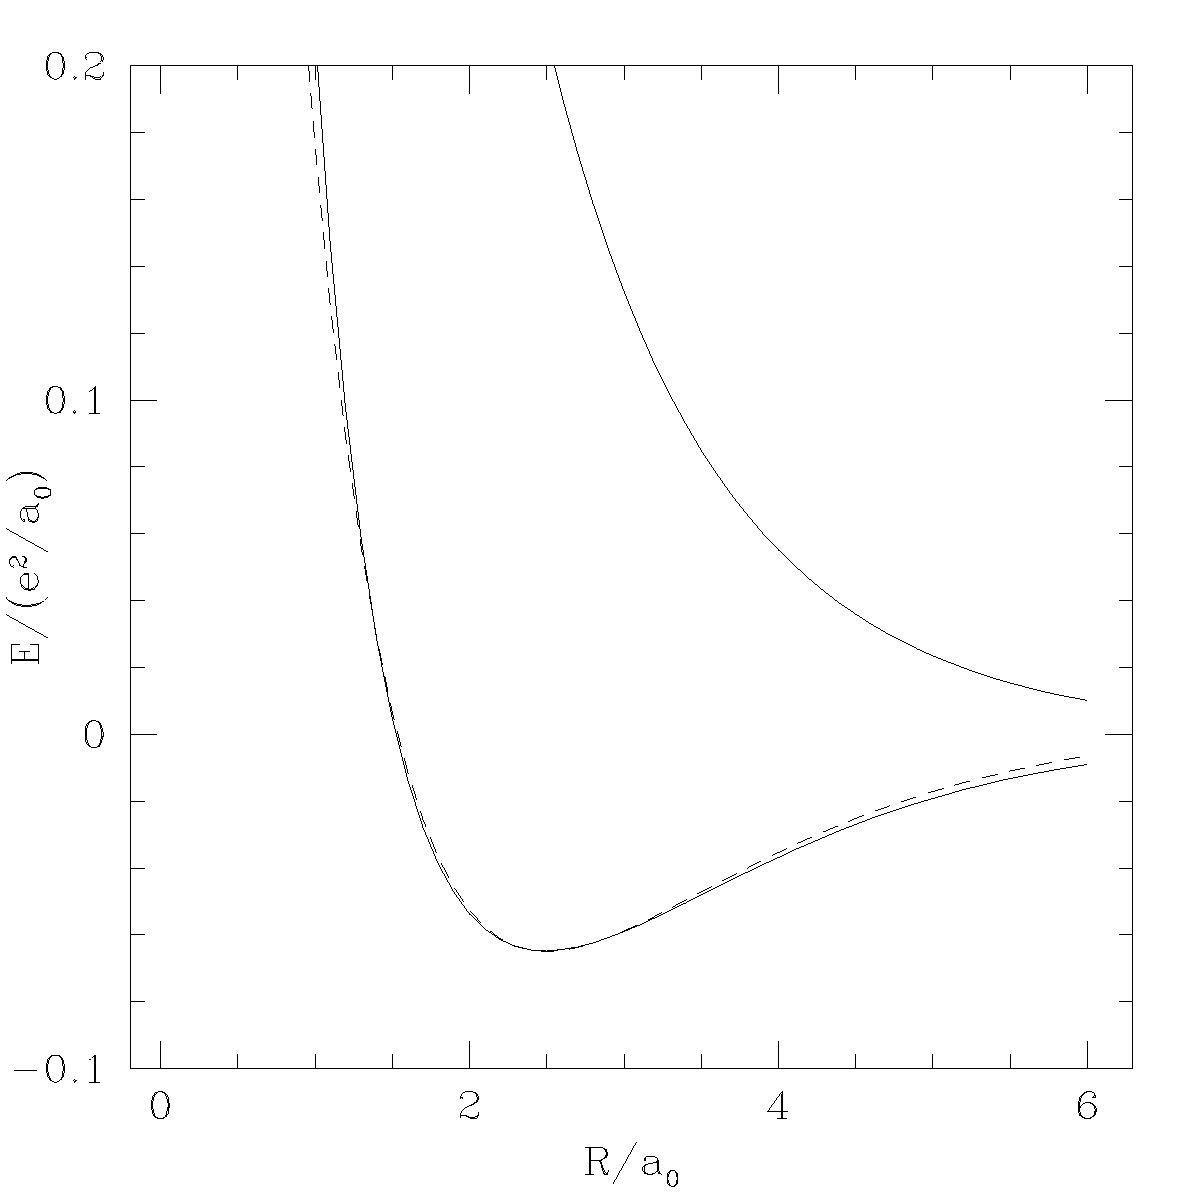
\includegraphics[width=0.45\textwidth]{h2p} 
\caption{$E_{u}$ (upper curve) and $E_g$ (lower curve) for
  H$_2^+$. The dashed curve is a well-fit Morse potential for $E_g(R)$.}
\label{fig:h2p}
\end{figure}
}
{
\begin{figure}
\centering
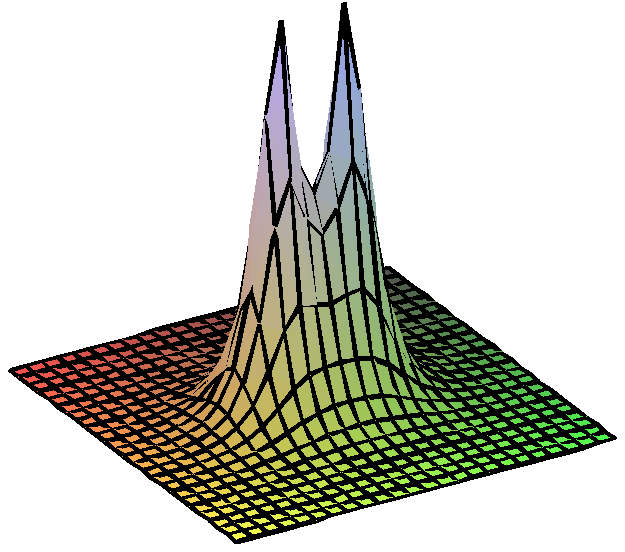
\includegraphics[width=0.45\textwidth]{psig} 
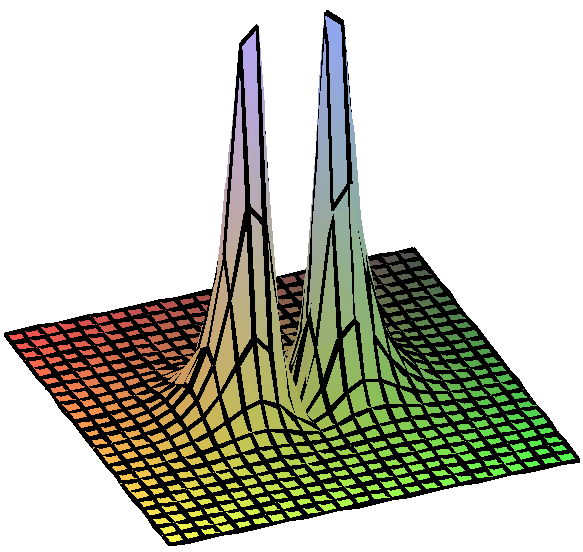
\includegraphics[width=0.45\textwidth]{psiu} 
\caption{$|\psi_g|^2$ (left) and $|\psi_u|^2$ (right) for H$_2^+$ with
  $R=2 a_0$.}
\label{fig:psiug}
\end{figure}
}

For molecules with more than one electron, we find that the Hund's rule
for the total spin of a system is reversed for molecules.  The states
with even parity (gerade) tend to bond.  Because the spatial wavefunction is
even with respect interchanging the electrons their spins must be
antiparallel. 

\section{Molecular Excitations}
\label{sec:molec-excit}
\index{molecular structure!excitations}

The energy states of molecule may be excited in three ways: {\em
  electronic}, {\em vibrational}, and {\em rotational}.  Let's start
  with the least energetic of these.

We can get a first-order understanding of the rotational states of a
molecule simply looking at the Schrodinger equation for the ions
\be 
\left [
-\frac{\hbar^2}{2 \mu_{AB}} \left ( \frac{d^2}{dR^2} -
\frac{L(L+1)}{R^2} \right )  + E_j({\bf R}) - E \right
] F_j({\bf R}) = 0 
\label{sec:molec-excit-1}\end{equation}
where we have solved the angular wavefunction in terms of spherical
harmonics like we did for hydrogen.  In Fig.~\ref{fig:h2p} we saw that
the function $E_j({\bf R})$ varies over atomic distances $\sim a_0$.
On the other hand because the mass of the ions is much larger than
that of the electrons we expect the wavefunction of the ions to be
localized in a region $\sim a_0 m/M \ll a_0$.  Over this small region
we can expand the function $E_j(R)$ about its minimum $R_0$
\begin{equation}
E_j(R) = E_j(R_0) + (R-R_0) \left [ \dd{E_j(R)}{R} \right ]_{R=R_0} +
\frac{1}{2} (R-R_0)^2 \left [ \frac{d^2 E_j(R)}{d R^2} \right
]_{R=R_0} + \cdots
\label{eq:580}
\end{equation}
where the second term vanishes because $R_0$ is the minimum so we have
\be 
\left [
-\frac{\hbar^2}{2 \mu_{AB}} \frac{d^2}{dR^2} -
\frac{\hbar^2}{2\mu_{AB}} \frac{L(L+1)}{R^2} + E_j(R_0) + \frac{1}{2}
k (R-R_0)^2 - E \right
] F_j({\bf R}) = 0 
\label{sec:molec-excit-2}\end{equation}
so we have
\begin{equation}
E = E_j(R_0) + \hbar \omega_0 \left ( v + \frac{1}{2} \right ) + \frac{\hbar^2}{2\mu_{AB}} \frac{L(L+1)}{R_0^2}
\label{eq:581}
\end{equation}
where $\omega_0 = (k/\mu_{AB})^{1/2}$ and 
we have treated the rotational motion of the molecule
perturbatively.  We have effectively ignored the possible centrifugal
stretching of the molecule.  If we were to include the stretching of
the molecule we would have
\begin{equation}
E_\rmscr{rot} = \frac{\hbar^2}{2\mu_{AB}} \frac{L(L+1)}{R_0^2} \left [
  1 - \frac{2\hbar^2 L(L+1)}{k \mu_{AB} R_0^4} \right ]
\label{eq:582}
\end{equation}

We can get dipole transitions between the different rotational states
if
\begin{equation}
|d| = Z_1 e r_1 + Z_2 e r_2 + |d_e| \neq 0 
\label{eq:583}
\end{equation}
and $\Delta L = \pm 1$.  We see that homonuclear diatomic molecules
cannot emit dipole radiation due to changes in their rotational state.
The energy of the radiation is given by
\begin{equation}
E_{L+1,L} = \frac{\hbar^2 (L+1)}{\mu_{AB} R_0^2} \left [ 1 - 4
    \frac{\hbar^2 (L+1)^2}{k \mu_{AB} R_0^4} \right ]
\label{eq:584}
\end{equation}
This energy is $\sim e^2/a_0 (m/\mu_{AB})$ or $\sim 10^{-3}$~eV.

The transitions between vibrational states has a typical energy of 
$\sim e^2/a_0 (m/\mu_{AB})^{1/2}$ or $\sim 10^{-1}$~eV.  If one
includes the centrifugal effects one finds that 
\begin{equation}
E_v = \hbar \omega_L \left ( v + \frac{1}{2} \right )
\label{eq:585}
\end{equation}
where
\index{Morse function}
\index{molecular structure!Morse function}
\begin{equation}
\omega_L \approx \mu_{AB}^{-1/2} \left [ k + \frac{3 \hbar^2
    L(L+1)}{\mu_{AB} R_0^4} \right ]^{1/2}
\label{eq:586}
\end{equation}
Morse found that the internuclear potential can often be well
approximated by a function of the form
\begin{equation}
E_n(R) = E_{n,0} + B_n \left \{ 1 - \exp \left[ \beta_n \left ( R -
  R_0 \right )\right ] \right \}^2
\label{eq:587}
\end{equation}
The energy eigenvalues of this potential are
\begin{equation}
E_{nv} = \hbar \omega_{n0} \left ( v + \frac{1}{2} \right ) -
\frac{\hbar^2 \omega_0^2}{4 B_n} \left ( v + \frac{1}{2} \right )^2.
\label{eq:588}
\end{equation}
The vibrational levels get closer together as $v$ increases and there
are a finite number of vibrational levels
\begin{equation}
0 \leq v \leq \frac{(2\mu_{AB} B_n)^{1/2}}{\beta_n \hbar} - \frac{1}{2}
\label{eq:589}
\end{equation}

The selection rules for vibrational transtions are again $|d|\neq 0$ but
also $d|d|/dR \neq 0$.  We can change the vibrational level by $\Delta
v=\pm 1$ and we must also have $\Delta L=L_\textrm{\scriptsize lower}-L_\textrm{\scriptsize upper}=+1$ ($P$ branch) or $\Delta
L=-1$ ($R$ branch) or if there is an component of electronic orbital
or spin angular momentum along the internuclear axis $\Delta L=0$ ($Q$ branch).

Fig.~\ref{fig:molecule_trans} shows the three branches for
roto-vibrational transitions, if we neglect the stretching of the
molecule.    We see that
for the $R$ branch the transition energy decreases with increasing $L$.
For the $Q$ branch it is constant, and for the $P$ branch the
transition energy increases with increase $L$.  The centrifugal stretching reduces the spacing of the
angular momentum energy levels for large values of $L$ (Eq.~\ref{eq:584}), but it
stiffens the spring constant of the vibrational statres (Eq.~\ref{eq:586}).  The latter
dominates, so the stretching effect
tends to make the transition energies increase with increasing $L$ for
large values of $L$.  Fig.~\ref{fig:COCar} depicts the
roto-vibrational spectrum of CO (the most commonly observed molecule
in astrophysics --- it isn't the most common, what is the most common
molecule and why isn't it commonly observed?) from samples of car
exhaust.  The CO molecule does not exhibit a $Q$-branch which would
appear at about 2140~cm$^{-1}$.

The Fortrat diagram (Fig.~\ref{fig:fortrat})
depicts the transition energies for various roto-vibrational
transitions as a function of the rotational quantum number $L$.  The
figure shows the expected behaviour, especially for the ``22''
transitions for which all three branches are depicted.  For small
values of $L$ the $Q$-branch has constant energy with $L$ and then
begins to increase with increasing $L$  The energy of the $P$-branch
transitions decreases with increasing $L$, and the opposite occurs
for the $R$ branch.

\begin{figure}
\begin{center}
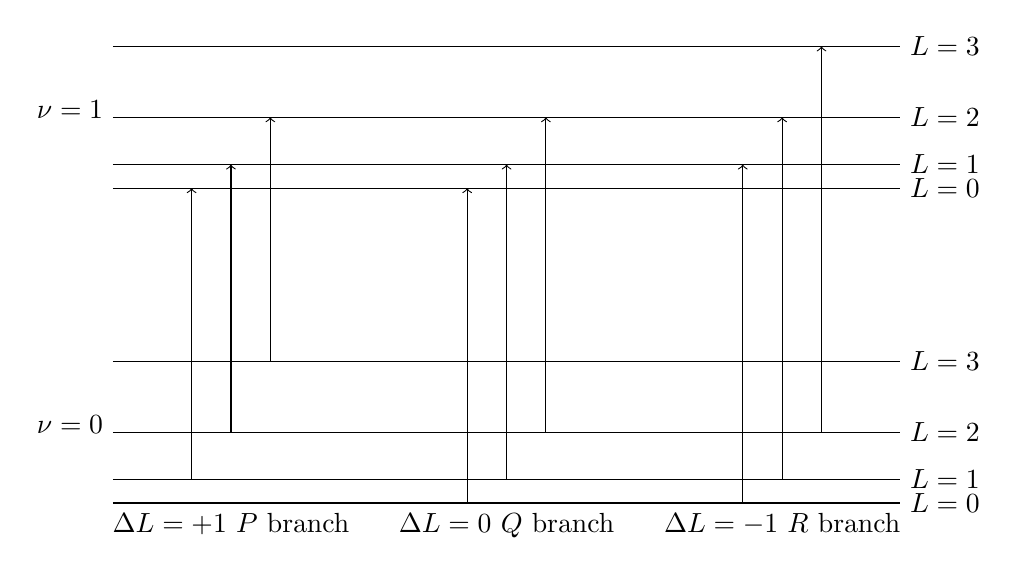
\begin{tikzpicture}
\foreach \nqn in {0,1}
  \foreach \lqn in {0,1,2,3} 
    \draw (0,\nqn*4+0.15*\lqn*\lqn+0.15*\lqn) -- (10,\nqn*4+0.15*\lqn*\lqn+0.15*\lqn) node [right] {$L=\lqn$};
\draw (0,5) node [left] {$\nu=1$} (0,1) node [left] {$\nu=0$};
\draw [->] (1,0.3) -- (1,4);
\draw [->] (1.5,0.9) -- (1.5,4.3);
\draw [->] (2,1.8) -- (2,4.9);
\draw (1.5,0) node [below] {$\Delta L=+1$ $P$ branch};
\draw [->] (4.5,0) -- (4.5,4);
\draw [->] (5,0.3) -- (5,4.3);
\draw [->] (5.5,0.9) -- (5.5,4.9);
\draw (5,0) node [below] {$\Delta L=0$ $Q$ branch};
\draw [->] (8,0) -- (8,4.3);
\draw [->] (8.5,0.3) -- (8.5,4.9);
\draw [->] (9,0.9) -- (9,5.8);
\draw (8.5,0) node [below] {$\Delta L=-1$ $R$ branch};
\end{tikzpicture}
\end{center}
\caption{Roto-Vibrational Transitions Neglecting Stretching}
\label{fig:molecule_trans}
\end{figure}

{\begin{figure}
\centering
\begin{tikzpicture}[scale=0.9]
\draw (0,0) node {
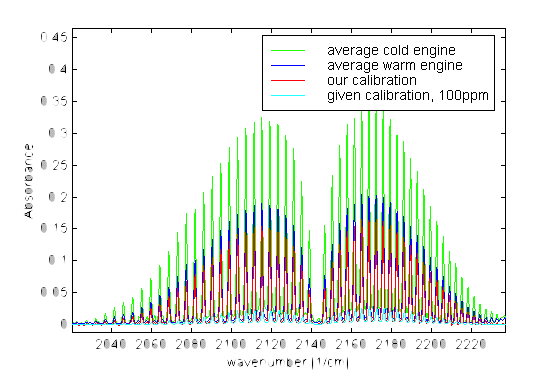
\includegraphics[width=0.9\textwidth,clip,trim=2.8cm 1.68cm 2.1cm 3.93cm]{CO_Car}
};
\draw [->] (-6.2,-3.25) -- (-6.2,3.05);
\draw [->] (-6.3,-3.15) -- (6.5,-3.15);
\draw (0,-3.6) node [below] {Wavenumber [cm$^{-1}$]};
\foreach \lam in {2040,2060,...,2220} 
   \draw (0.05893*\lam-125.5,-3.2) node [below] {\lam};
\foreach \abs in {0,0.1,0.2,0.3} 
   \draw (-6.2,18.6*\abs-3.15) node [left] {\abs};
\end{tikzpicture}
\caption{Absorption vs.\ Wavenumber for FTIR Spectroscopy of CO in car
  exhaust from {\tt
    http://home.swipnet.se/$\sim$w-74877/ftir/ftir.htm}.  Green is a
  cold engine, blue is a warm engine, red is a calibration reading and
cyan is a 100ppm calibration.}
\label{fig:COCar}
\end{figure}}
{\begin{figure}
\centering
\begin{tikzpicture}[scale=0.9]
\draw (0,0) node {
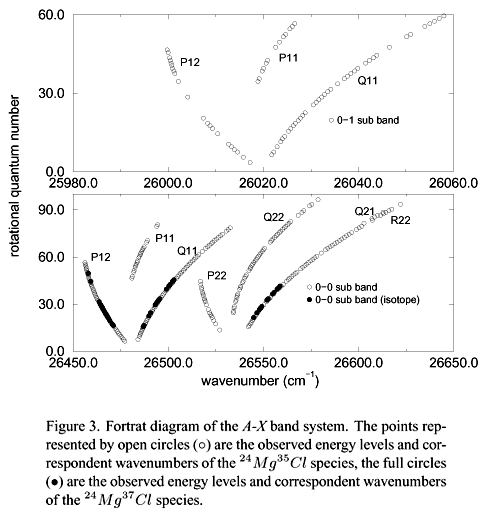
\includegraphics[width=0.9\textwidth,clip,trim=1cm 4.6cm 0 6.7cm]{fortrat.png} 
};
\draw (-6.5,0.3) node [rotate=90] {Rotational Quantum Number};
\end{tikzpicture}
\caption{A Fortrat diagram for $^{24}$Mg$^{35}$Cl and
  $^{24}$Mg$^{37}$Cl (isotope) from Gutterres et al. (2003),
  Braz. J. Phys. vol. 33}
\label{fig:fortrat}
\end{figure}}

In general each vibration transition includes a rotational transition
as well so one gets group of transitions.  The final wrinkle is that
electronic transitions in molecules whose energy $\sim 1$~eV
necessarily include changes in the rotational and vibrational state of
the molecule.  The general electronical-vibrational-rotational
spectrum takes the form of bands which can be resolved into individual
lines if the broadening is weak.

\section{Problems}
\begin{enumerate}

\item{\bf The Number of Levels}

I fit a Morse function to the potential of  H$_2^+$.  The parameters
were
\begin{equation}
E_{n,0} = -0.065 \frac{e^2}{a_0}, B_n = 0.07 \frac{e^2}{a_0}, \beta_n
= 0.7 a_0^{-1}, R_0 = 2.5 a_0
\label{eq:590}
\end{equation}
How many vibrational levels does H$_2^+$ have?   How many rotational
levels does each vibrational level typically have?

\item{\bf Nuclear Overlap}

Consider two deuterons bound by a single electron as in question (1).
What is the probability that the two deuterons lie on top of each
other, {\ie} that $R<4$~fermi, the diameter of the deuteron?   What is the
probability if the two deuterons are bound by a single muon, $m_\mu
\approx 207 m_e$?  You can find the eigenfunctions of the Morse
potential on Wikipedia.

If you assume that whenever the deuterons overlap they fuse and that
you get to ``roll the dice'' once each oscillation period, calculate
the fusion rate in both cases.

\item{\bf Stretching}

Calculate the value of $L$ for which the energy of the $P$ branch
transitions begins to increase.

\item{\bf Temperature}

Using the results depicted in Fig.~\ref{fig:COCar}, estimate the
temperature of the hot and cold car exhaust and the relative
concentration of CO in the two cases.
\end{enumerate}

%%% Local Variables: 
%%% mode: latex
%%% TeX-master: "book"

\chapter{Fluid Mechanics}
\label{cha:fluid-mechanics}\index{fluid mechanics}
\section{Phase-Space Density}
\label{sec:phase-space-density}
\index{fluid mechanics!phase-space density}
\index{phase-space density}

The phase-space density of particles gives the number of particles in
an infinitesimal region of phase space,
\begin{equation}
d N = f(x^\alpha,{\bf p}) d^3 {\bf x} d^3 {\bf p}
\label{eq:591}
\end{equation}
If there is no dissipation, the phase-space density 
along the trajectory of a particular particle
is given by
\begin{equation}
\dd{f}{\tau} = {\cal C}
\label{eq:592}
\end{equation}
where ${\cal C}$ accounts for two-body interactions between
particles.   This is known as the Boltzmann equation. If there are no collisions, ${\cal C}=0$, so
\index{Lioville's theorem}
\index{fluid mechanics!Lioville's theorem}
\begin{equation}
\dd{f}{\tau} = 0.
\label{eq:593}
\end{equation} 
This is called Lioville's theorem or the collisionless Boltzmann
equation.  This limit applies in galactic dynamics.  Here we are
interested in particles in a gas that do collide so we expand out the
derivative along the flow lines to get
\begin{equation}
\pp{f}{t} + {\bf v} \cdot \nabla f + {\bf F} \cdot \pp{f}{{\bf p}} =
   {\cal C}
\label{eq:594}
\end{equation}
where ${\bf F}$ is a force that accelerates the particles.  The
collision term ${\cal C}$ must now be expressed in the lab frame of
this equation that is no longer manifestly covariant.  The requirement
of no dissipation tells us that $\nabla_{\bf p} \cdot {\bf F} = 0$.

We would like to define some quantities that are integrals over
momentum space that transform simply under Lorentz transformations.
We derived earlier (\S~\ref{sec:transf-radi-transf}) that
\begin{equation}
\frac{d^3 {\bf p}}{p_t} = \frac{d^3{\bf p}'}{p'_t}.
\label{eq:595}
\end{equation}
We also know that $E_{\bf p} = p_t = (p^2 c^2 + m^2 c^4)^{1/2}$
so
\begin{equation}
\frac{d^3 {\bf p}}{E_{\bf p}} = \rmmat{Lorentz Invariant}
\label{eq:596}
\end{equation}
so we can define various integrals
\begin{equation}
\frac{n(x^\alpha)}{{\bar E}_\rmscr{har}(x^\alpha)} \equiv \int \frac{d^3 {\bf
    p}}{E_{\bf p}} f(x^\alpha, {\bf p})
\label{eq:597}
\end{equation}
that transforms as a scalar where $n(x^\alpha)$ is the number density..  Unfortunately, there isn't much that one
can do with it.  One could use it as the source for a scalar theory of
gravity, but it would violate the equivalence principle.

\subsection{Particle Current}
\label{sec:particle-current}
\index{fluid mechanics!particle current}
Next let's define
\begin{equation}
J^\mu (x^\alpha)  \equiv c \int \frac{d^3 {\bf p}}{E_{\bf p}} p^\mu f(x^\alpha, {\bf p}).
\label{eq:598}
\end{equation}
Because this is simply the sum of things that transform as a
four-vector, $J^\mu$ also transforms as a four-vector.  Let's look at
it component by component
\begin{eqnarray}
J^0(x^\alpha) &=& \int \frac{d^3 {\bf p}}{E_{\bf p}} c p^0 f(x^\alpha, {\bf p}) = 
\int d^3 {\bf p} f(x^\alpha, {\bf p}) =  n(x^\alpha) \\
{\bf J}(x^\alpha) &=& \int \frac{d^3 {\bf p}}{E_{\bf p}} c {\bf p}
f(x^\alpha, {\bf p}) = \frac{1}{c} \int d^3 {\bf p} {\bf v} f(x^\alpha, {\bf
  p}) =  \frac{\langle {\bf v} \rangle}{c} n(x^\alpha) 
\label{eq:599}
\end{eqnarray}
If we assume that the scattering (${\cal C}$) conserves energy, momentum
and particles we have
\begin{equation}
J^{\mu}_{~~,\mu} = \pp{J^\mu}{x^\mu} = n \langle \nabla_{\bf p} \cdot {\bf F} \rangle.
\label{eq:600}
\end{equation}
We can prove this simply by integrating Eq.~\ref{eq:594} over $d^3 {\bf p}$.
The first two terms yield the left-hand side of the equation above.  
The third term gives the right-hand side.  This vanishes
as long as 
\begin{equation}
\nabla_{\bf p} \cdot {\bf F} = 0 
\label{eq:601}
\end{equation}
and the right-hand side vanishes if the scattering conserves energy
and momentum.

Let's define ${\bf V}=\langle {\bf v} \rangle$ and write out Eq.~\ref{eq:601}
by components,
\begin{equation}
\pp{n}{t} + \nabla \cdot \left (n {\bf V} \right ) = 0 
\label{eq:602}
\end{equation}
or
\begin{equation}
\pp{\rho}{t} + \nabla \cdot \left (\rho {\bf V} \right ) = 0 
\label{eq:603}
\end{equation}
where $\rho=mn$ where $m$ is the rest mass of the individual particles.
This is the continuity equation.  This must hold true regardless of
the nature of the force, {\em i.e.} even if $\nabla_{\bf p} \cdot F
\neq 0$.  Because Eq.~(\ref{eq:600}) is consistent with the Lioville
equation (Eq.~\ref{eq:593}) and more generally with the Boltzmann
equation (Eq.~\ref{eq:592}) and $J^\mu_{;\mu}=0$ if particles are
conserved,  the Lioville and Boltzmann equations cannot hold if 
$\nabla_{\bf p} \cdot F \neq 0$ and particles are conserved.

\subsection{Stress Tensor}
\label{sec:stress-tensor}
\index{fluid mechanics!stress tensor}

Let's construct a tensor from the distribution function
\begin{equation}
T^{\mu\nu} (x^\alpha)  \equiv c^2 \int \frac{d^3 {\bf p}}{E_{\bf p}}
p^\mu p^\nu f(x^\alpha, {\bf p}).
\label{eq:604}
\end{equation}
this is called the energy-momentum tensor or stress tensor of the
system.  Let's take one of the indices to be zero
\begin{equation}
T^{\mu 0} (x^\alpha) = c^2 \int \frac{d^3 {\bf p}}{E_{\bf p}}
p^\mu \frac{E_{\bf p}}{c} f(x^\alpha, {\bf p}) = 
c \int d^3 {\bf p} p^\mu f(x^\alpha, {\bf p})
\label{eq:605}
\end{equation}
which is the product of the total four momentum of the particle per
unit volume with $c$.  $T^{00}(x^\alpha)$ gives the energy-density and
the component $T^{0\mu}(x^\alpha)$ gives the density of the 
$\mu-$component of the three-momentum.

We are free to fix a Lorentz frame that is moving with the material
such that $J^\mu=0$ for $\mu\neq 0$.  If we are willing to neglect
effects that depend on the gradient of the velocity (such as
viscosity or heat conduction) we can define this frame globally.  Furthermore, let's
assume that the distribution function is isotropic in the momentum.
Fluids for which this is possible are called {\em ideal fluids}.  In
this case we have
\begin{equation}
J^0 = 4\pi \int_0^\infty p^2 f(p) dp, J^\mu = 0 
\label{eq:606}
\end{equation}
and
\begin{equation}
\epsilon = T^{00} = 4\pi \int_0^\infty p^2 E(p) f(p) dp, T^{0\mu}=0
\label{eq:607}
\end{equation}
The space-space part of the energy-momentum tensor must be symmetric,
isotropic and a three-dimensional tensor (a matrix).  The only tensor
that works is
\begin{equation}
T^i_{~~j} = P \delta^i_{~~j}
\label{eq:608}
\end{equation}
where
\begin{equation}
T^i_{~~i} = P \delta^i_{~~i} = 3 P = c^2 \int \frac{d^3 {\bf p}}{E_p} p^2 f(p) = 
4 \pi c^2 \int_0^\infty \frac{p^4}{E(p)} f(p) dp
\label{eq:609}
\end{equation}
so
\begin{equation}
P = \frac{4 \pi}{3} c^2 \int_0^\infty \frac{p^4}{E(p)} f(p) dp.
\label{eq:610}
\end{equation}
Notice that the trace of the energy-momentum tensor $T^\mu_{~~\mu}$ is a
scalar.  In fact it is simply the product of $m^2 c^4$ with the scalar
density defined in Eq.~\ref{eq:597}.

Let's look at the non-relativistic limit of the energy-momentum tensor.
Let's take $T^{00} = mc^2 n + \epsilon_\rmscr{nr}$ where
\begin{equation}
T^{00} = 4\pi \int_0^\infty p^2 \left (mc^2 + \frac{p^2}{2m} \right )
f(p) dp = n mc^2 + \epsilon_\rmscr{nr}
\label{eq:611}
\end{equation}
where
\begin{equation}
\epsilon_\rmscr{nr} = 4\pi \int_0^\infty p^2 \frac{p^2}{2m} f(p) dp =
\frac{2\pi}{m} \int_0^\infty p^4 f(p) dp.
\label{eq:612}
\end{equation}
Let's look at the non-relativistic limit of the pressure
\begin{equation}
P_\rmscr{nr} = \frac{4 \pi}{3} c^2 \int_0^\infty \frac{p^4}{mc^2}
f(p) = \frac{4\pi}{3m} \int_0^\infty p^4 f(p) dp
\label{eq:613}
\end{equation}
so $\epsilon_\rmscr{nr} = \frac{3}{2} P_\rmscr{nr}$.  Now let's take
the opposite limit
\begin{equation}
\epsilon_\rmscr{ur} = T^{00} = 4 \pi \int_0^\infty p^2 (p c) f(p) dp,
p_\rmscr{ur} = \frac{4\pi}{3} c^2 \int_0^\infty \frac{p^4}{pc} f(p) dp
\label{eq:614}
\end{equation}
so $P=\epsilon/3$ in the ultrarelativistic limit.  We can transform
from this special frame to a frame where the fluid moves and get
\begin{equation}
T^\mu_{~~\nu} = (P + \epsilon) U^\mu U_\nu - P \delta^\mu_{~~\nu}
\label{eq:615}
\end{equation}
and 
\begin{equation}
J^\mu = n_\rmscr{prop} U^\mu
\label{eq:616}
\end{equation}
$n_\rmscr{prop}$ is the number density of the particles in a frame
moving with the particles and $U^\mu$ is the bulk four-velocity of the
fluid. 

We can calculate the evolution of this tensor by integrating over
Lioville's equation times $p^\mu$ to get
\begin{equation}
T^{\mu\nu}_{~~~~,\nu} = \pp{T^{\mu\nu}}{x^\nu} = \left \{ \begin{array}{ll}
n \langle {\bf v} \cdot {\bf F} \rangle, & \mu = 0 \\
c n \langle {\bf F} \rangle, & \mu > 0 
\end{array} \right . .
\label{eq:617}
\end{equation}
We prove this by integrating Eq.~\ref{eq:594} times $p^\mu$ over $d^3{\bf p}$.
The zero-component is simply the work performed by the force on the
particles in the volume.  The other components account for the change
in the momentum of the particles.

\subsubsection{Non-relativistic limit}
\label{sec:non-relat-limit}
\index{fluid mechanics!non-relativistic}

Let's examine what this equation means in the non-relativistic limit,
\begin{equation}
T^{00} = c^2 \int d^3 {\bf p} f(p) m c^2 \left ( 1 +
\frac{1}{2}\frac{v^2}{c^2} \right )= \rho c^2 + \int d^3 p f \left (
\frac{1}{2} m v^2 \right ) = \rho c^2 + n \langle E \rangle
\label{eq:618}
\end{equation}
and
\begin{equation}
T^{0\nu} = c^2 \int d^3 {\bf p} f m c v^\nu \left ( 1 +
\frac{1}{2}\frac{v^2}{c^2}\right ) = \left ( \rho c {\bf V} +
\frac{1}{c} {\bf q} \right )^{\nu}
\label{eq:619}
\end{equation}
where
\begin{equation}
{\bf q} = \int d^3 {\bf p} \left ( \frac{1}{2} m v^2 \right ) {\bf v} f
\label{eq:620}
\end{equation}
is the flux of kinetic energy.  The first term is the flux of
rest-mass energy.  Finally for the space-space part we have
\begin{equation}
T^{\mu\nu} = \int d^3{\bf p} m v^\mu v^\nu f.
\label{eq:621}
\end{equation}
Let's look at the zero-component of Eq.~\ref{eq:617} 
\begin{equation}
\frac{1}{c} \pp{}{t} \left ( \rho c^2 + n \langle E \rangle \right ) + \nabla
\cdot \left ( \rho c {\bf V} + \frac{\bf q}{c} \right ) = n \langle
      {\bf v} \cdot {\bf F} \rangle
\label{eq:622}
\end{equation}
We can subtract $c$ times the continuity equation to get
\begin{equation}
\pp{n \langle E \rangle}{t} + \nabla \cdot {\bf q} = n \langle
      {\bf v} \cdot {\bf F} \rangle.
\label{eq:623}
\end{equation}
This ensures conservation of energy.  We can divide the energy from
the bulk flow from the random kinetic energy of the fluid
\begin{equation}
N \langle E \rangle = N \left \langle \frac{1}{2} m \left ( {\bf V} + {\bf v}_r
\right )^2 \right \rangle = \frac{1}{2} \rho V^2 + \frac{1}{2} \rho
\langle v_r^2 \rangle = \frac{1}{2} \rho V^2 + \frac{3}{2} N T,
\label{eq:624}
\end{equation}
defining the temperature $T$ of the fluid.

The spatial part of Eq.~\ref{eq:618} gives
\begin{equation}
\frac{1}{c} \pp{}{t} \left ( \rho c {\bf V} + \frac{\bf q}{c} \right
)^i + \pp{T^{ik}}{x^k} = n \langle {\bf F} \rangle.
\label{eq:625}
\end{equation}
The first term in the parentheses is larger by a factor of $c^2$ so to
lowest order we have
\begin{equation}
\pp{}{t} \left ( \rho V^i \right ) + \pp{T^{ik}}{x^k} = n \langle {\bf F} \rangle.
\label{eq:626}
\end{equation}
This is equivalent to neglecting the momentum carried by the flow of 
energy.

\section{Ideal Fluids}
\label{sec:ideal-fluids}
\index{fluid mechanics!ideal fluids}
\index{ideal fluids}
For an ideal fluid we found that the stress tensor took a particular
form,
\begin{equation}
T^{\mu\nu} = (p + \epsilon) U^\mu U^\nu - P g^{\mu\nu}
\label{eq:627}
\end{equation}
In the non-relativistic limit we find that space-space components are
\begin{equation}
T_{ik} = \rho V_i V_k + P \delta_{ik}
\label{eq:628}
\end{equation}
and
\begin{equation}
{\bf q} = \left [ \frac{1}{2} V^2 + w \right ] \rho {\bf V}
\label{eq:629}
\end{equation}
where $w=(\epsilon + P)/\rho$ is the heat function (enthalpy) per
unit mass of the fluid. Notice that there is no energy flow without
bulk motion.  If we substitute this into the equations
derived earlier we get
\begin{equation}
\pp{\rho}{t} + \nabla \cdot \left ( \rho {\bf V} \right ) = 
\pp{\rho}{t} + \left ( {\bf V} \cdot \nabla \right ) \rho 
+ \rho \nabla \cdot {\bf V} =
\dd{\rho}{t} + \rho \nabla \cdot {\bf V} = 0
\label{eq:630}
\end{equation}
and
\begin{equation}
\pp{{\bf V}}{t} + \left ( {\bf V} \cdot \nabla \right ) {\bf V} =
\dd{\bf V}{t} = -\frac{\nabla P}{\rho} + \frac{\langle {\bf F} \rangle}{m}
\label{eq:631}
\end{equation}

In the ideal fluid, no heat is tranferred between different parts of
the fluid, so if we denote $s$ as the entropy per unit rest mass we have
\begin{equation}
\dd{s}{t} = 0
\label{eq:632}
\end{equation}
for a bunch of fluid; therefore, we also have a continuity equation
for the entropy
\begin{equation}
\pp{(\rho s)}{t} + \nabla \cdot \left ( \rho s {\bf v} \right ) = 0.
\label{eq:633}
\end{equation}
We can use the continuity equation for particle number to simplify
this further,
\begin{equation}
\rho \pp{s}{t} + {\bf v} \cdot \nabla (\rho s) = 0.
\label{eq:634}
\end{equation}

\subsection{Isentropic flows}
\label{sec:isentropic-flows}
\index{fluid mechanics!isentropic flows}
\index{isentropic flows}

An important case of adiabatic flows is when the entropy $s$ is
initially constant.  In such an isentropic flow, the entropy will
remain constant and we can derive some additional useful forms of
Eq.~\ref{eq:631}.

From the definition of the work function $w$ and thermodynamics we
know that
\begin{equation}
d w = T ds + \frac{1}{\rho} dp = \frac{dp}{\rho}
\label{eq:635}
\end{equation}
because the entropy is constant, $ds=0$.  We get
\begin{equation}
\pp{{\bf V}}{t} + \left ( {\bf V} \cdot \nabla \right ) {\bf V} =
\dd{\bf V}{t} = -\nabla w + \frac{\langle {\bf F} \rangle}{m}
\label{eq:636}
\end{equation}
From vector analysis we know
\begin{equation}
\frac{1}{2} \nabla v^2 = {\bf v} \times (\nabla \times {\bf v}) + ({\bf
  v} \cdot \nabla ) {\bf v}
\label{eq:637}
\end{equation}
and we can get
\begin{equation}
\pp{{\bf V}}{t} + \frac{1}{2} \nabla v^2 - {\bf v} \times (\nabla
\times {\bf v} ) = -\nabla w + \frac{\langle {\bf F} \rangle}{m}.
\label{eq:638}
\end{equation}
If we take the curl of both sides we find that
\begin{equation}
\pp{}{t}\left ( \nabla \times {\bf V} \right ) = \nabla \times \left( {\bf V}
\times (\nabla \times {\bf V} ) \right ) + \nabla \times \frac{\langle
  {\bf F} \rangle }{m}
\label{eq:639}
\end{equation}
$\omega = \nabla \times {\bf V}$ is called the vorticity.

If we assume that ${\bf F}/m = -\nabla \phi$ which is often the case,
we find that if the flow in an isentropic, ideal fluid is initially
irrotational it will remain irrotational.

We can go further than this.  Let's define
\begin{equation}
\Gamma = \oint {\bf v} \cdot d{\bf l}
\label{eq:640}
\end{equation}
taken along some closed contour that moves with the fluid.   Let's
calculate
\begin{equation}
\dd{\Gamma}{t} = \dd{}{t}\oint {\bf v} \cdot d{\bf l} = \dd{}{t} \oint {\bf v}
\cdot \delta {\bf r} = \oint \dd{\bf v}{t} \cdot \delta {\bf r}
+ \oint {\bf v} \cdot \dd{}{t} \delta {\bf r}.
\label{eq:641}
\end{equation}
Because $\delta {\bf r}$ is the difference between two positions
moving with the fluid we have
\begin{equation}
{\bf v} \cdot \dd{}{t} \delta {\bf r} = {\bf v} \cdot \delta \dd{\bf
  r}{t} = {\bf v} \cdot \delta {\bf v} = \delta v^2
\label{eq:642}
\end{equation}
so
\begin{equation}
\dd{}{t}\oint {\bf v} \cdot d{\bf l} =\oint \dd{\bf v}{t} \cdot d {\bf
  l} = \oint \left ( -\nabla w + \frac{\langle {\bf F} \rangle}{m}
\right ) d {\bf l} = 0 
\label{eq:643}
\end{equation}
if ${\bf F}/m = -\nabla \phi$, so the circulation around a contour
moving with the fluid is constant if the flow is isentropic.

\begin{figure}
\begin{center}
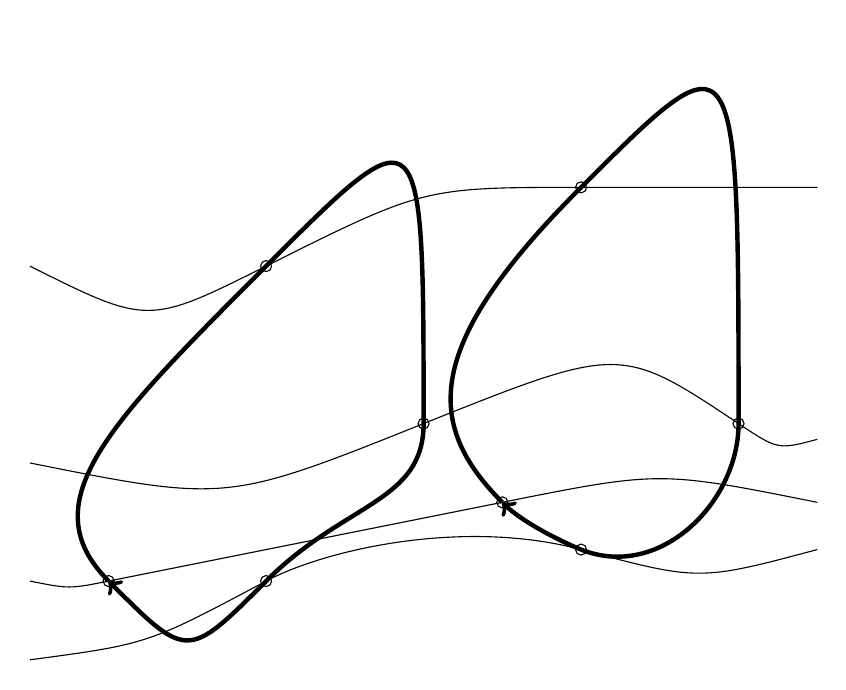
\begin{tikzpicture}
\draw [->,ultra thick] (0,0) .. controls (-1,1) and (0,2) .. (2,4) .. controls (4,6)
.. (4,2) .. controls (4,1) and (3,1) .. (2,0) .. controls (1,-1)
.. (0,0);
\draw [->,ultra thick] (5,1) .. controls (4,2) and (4,3) .. (6,5) .. controls (8,7)
.. (8,2) .. controls (8,1) and (7,0) .. (6,0.4) .. controls (5.75,0.5)
and (5.25,0.75) .. (5,1);
\draw [->] (-1,0) .. controls (-0.5,-0.1) .. (0,0) circle (2pt)
.. controls (0.5,0.1) .. (5,1) circle (2pt) .. controls (7,1.4) .. (9,1);
\draw [->] (-1,4) .. controls (0.5,3.25) .. (2,4) circle (2pt)
.. controls (4,5) .. (6,5) circle (2pt) -- (9,5);
\draw [->] (-1,1.5) .. controls (1.5,1) .. (4,2) circle (2pt)
.. controls (6.5,3) .. (8,2) circle (2pt) .. controls (8.5,1.66667) .. (9,1.8);
\draw [->] (-1,-1) .. controls (0.5,-0.8) .. (2,0) circle (2pt)
.. controls (2.75,0.4) and (4.5,0.8) .. (6,0.4) circle (2pt) .. controls (7.5,0) .. (9,0.4);
\end{tikzpicture}
\caption{The circulation around a close contour (bold lines) that
  travels with the fluid along the streamlines (light lines) is
  conserved if the fluid is isentropic.}
\end{center}
\end{figure}

\subsection{Hydrostatics}
\label{sec:hydrostatics}
\index{fluid mechanics!hydrostatics}
\index{hydrostatics}
Let's assume that the fluid is not moving.  If we look at Eq.~\ref{eq:632} we
get the equation of hydrostatic equilibrium.  Let's further suppose
that the force is derived from a potential, we obtain,
\begin{equation}
\frac{\nabla P}{\rho} = - \nabla \phi.
\label{eq:644}
\end{equation}
Let's take the divergence of both sides
\begin{equation}
\nabla \cdot \left ( \frac{\nabla p}{\rho} \right ) = -\nabla^2 \phi
= -4\pi G \rho
\label{eq:645}
\end{equation}
and in spherical coordinates we have
\begin{equation}
\frac{1}{r^2} \dd{}{r} \left ( \frac{r^2}{\rho} \dd{p}{r} \right ) =
-4\pi G \rho.
\label{eq:646}
\end{equation}
An interesting and important case is when the fluid is isentropic as
well, then we have
\begin{equation}
\nabla w = -\nabla \phi.
\label{eq:647}
\end{equation}
and
\begin{equation}
\nabla^2 w = -4\pi G \rho
\label{eq:648}
\end{equation}
If we look at the Eq.~\ref{eq:648} and imagine that the fluid is rotating we
have an extra term,
\begin{equation}
\nabla w = -\nabla \phi + \Omega^2({\bf r}) {\bf R}
\label{eq:649}
\end{equation}
where ${\bf R}$ is a vector pointing from the rotation axis to 
the point in the fluid.  Let's take the curl of both sides to get
\begin{equation}
0 = 0 + \nabla \times \left ( \Omega^2({\bf r}) {\bf R} \right )
\label{eq:650}
\end{equation}
which tells us that
\begin{equation}
\Omega ( {\bf r} ) = \Omega(R)
\label{eq:651}
\end{equation}
or that isentropic stars must have constant angular velocity on
cylindrical surfaces.

\subsection{Really Little Sound Waves}
\label{sec:really-little-sound}
\index{sound waves}
\index{fluid mechanics!sound waves}
The next order of complexity is to assume that the fluid is at rest
with a small perturbation and to see what the perturbation does.  We
have 
\begin{equation}
\pp{\rho}{t} + \nabla \cdot (\rho {\bf V}) = \pp{\rho'}{t} + \rho_0
\nabla \cdot {\bf V}' = 0 
\label{eq:652}
\end{equation}
and 
\begin{equation}
\pp{{\bf V}}{t} + \left ( {\bf V} \cdot \nabla \right ) {\bf V} =
\dd{\bf V}{t} + \frac{\nabla P}{\rho} =
\pp{{\bf V}'}{t} + \frac{\nabla P'}{\rho_0} = 0.
\label{eq:653}
\end{equation}
We can write $P' = (\partial P/\partial \rho)_s \rho'$ and rewrite the
continuity equation to get
\begin{equation}
\pp{P'}{t} + \rho_0 \left ( \pp{P}{\rho} \right )_s \nabla \cdot {\bf
  V'} = 0
\label{eq:654}
\end{equation}
Let's take the divergence of the Euler equation to get
\begin{equation}
\pp{{\bf \nabla \cdot V}'}{t} + \frac{\nabla^2 P'}{\rho_0} = 0.
\label{eq:655}
\end{equation}
and the time derivative of the continuity equation to get
\begin{equation}
\pp{^2 P'}{t^2} + \rho_0 \left ( \pp{P}{\rho} \right )_s \nabla \cdot \pp{\bf
  V'}{t} = 0.
\label{eq:656}
\end{equation}
Finally we put the two together to get
\begin{equation}
\pp{^2 P'}{t^2} - \left ( \pp{P}{\rho} \right )_s \nabla^2 P' = 0.
\label{eq:657}
\end{equation}
This is a wave equation with a sound speed of $c_s^2 = (\partial
P/\partial \rho)_s$.  Let's take a solution to this equation for the
pressure,
\begin{equation}
P' = p' \exp[i({\bf k} \cdot {\bf r} - \omega t)]
\label{eq:658}
\end{equation}
with $k^2 c_s^2=  \omega^2$ and calculate the velocity of the fluid
\begin{equation}
{\bf V}' = {\bf v}' \exp[i({\bf k} \cdot {\bf r} - \omega t)]
\label{eq:659}
\end{equation}
From Eq.~\ref{eq:654} we get
\begin{equation}
- \omega {\bf v}' +  \frac{p'}{\rho_0} {\bf k} = 0
\label{eq:660}
\end{equation}
and from Eq.~\ref{eq:655} we get
\begin{equation}
- \omega p' +  \rho_0 c_s^2 {\bf k} \cdot {\bf v'} = 0.
\label{eq:661}
\end{equation}
Combining these results gives
\begin{equation}
- \omega {\bf v}' +  \frac{c_s^2 {\bf k} \cdot {\bf
    v'}}{\omega} {\bf k} =0
\label{eq:662}
\end{equation}
and rearranging
\begin{equation}
{\bf v}' = \frac{c_s^2 {\bf k} \cdot {\bf v'}}{\omega^2} {\bf
  k} = v' \frac{\bf k}{k}.
\label{eq:663}
\end{equation}
Therefore, the fluid is displaced in the direction of the propagation
of the wave; it is a longitudinal wave.

\subsection{Steady Supersonic Flow}
\label{sec:steady-supers-flow}
\index{fluid mechanics!supersonic flow}
\index{supersonic flow}
Many disturbances travel through a fluid at a finite speed (changes in
the entropy or vorticity move with the fluid).  If the fluid itself
travels faster than the speed of sound, a disturbance starting at
particular point only can travel downstream so the upsteam flow cannot
know about it.  A flow can become supersonic abruptly as in a
shock or continuously.  We will examine this latter case here.

Let's imagine that a fluid is flowing through a pipe of variable cross
section $A(x)$ and that the flow is steady so that all partial time
derivatives vanish.  We can write the continuity equation as $\rho v
A=$constant.  The Euler equation becomes
\begin{equation}
v \dd{v}{t} = - \frac{1}{\rho} \dd{p}{t} = -\frac{c_s^2(\rho)}{\rho} \dd{\rho}{t}
\label{eq:664}
\end{equation}
where we have assumed that the fluid flows in the $x-$direction.  From
the continuity equation we know
\begin{equation}
-\frac{1}{A} \dd{A}{t} = \frac{1}{\rho v} \dd{(\rho v)}{t} 
= \frac{1}{\rho v} \left ( v \dd{\rho}{t} + \rho \dd{v}{t}  \right ) .
\label{eq:665}
\end{equation}
We can combine the two equations to get
\index{fluid mechanics!de Laval nozzle}
\index{de Laval nozzle}
\begin{equation}
\dd{\ln A}{t} = \frac{c_s^2}{v^2} \left ( 1 -
\frac{v^2}{c_s^2} \right ) \dd{\ln \rho}{t} = \frac{p}{\rho v^2}  \left ( 1 -
\frac{v^2}{c_s^2} \right )\dd{\ln p}{t} = - \left ( 1 -
\frac{v^2}{c_s^2} \right ) \dd{\ln v}{t}.
\label{eq:deLaval}
\label{eq:666}
\end{equation}
If $v<c_s$ we have the following situation,
\begin{itemize}
\item If the area of the pipe decreases (nozzle) in the direction of
  the flow, the velocity increases and the pressure and density
  decrease.
\item If the area of the pipe increases (diffuser) in the direction 
  of the flow,  the velocity decreases and the pressure and density increase.
\end{itemize}
On the other hand if the flow is supersonic ($v>c_s$) we have
\begin{itemize}
\item If the area of the pipe decreases (nozzle) in the direction of
  the flow, the velocity decreases and the pressure and density
  increase.
\item If the area of the pipe increases (diffuser) in the direction 
  of the flow,  the velocity increases and the pressure and density 
  decrease.
\end{itemize}

If we have a tube in which the flow is initially subsonic and the area
of the tube decreases, the flow will accelerate.  If the area of the
tube increases again the flow will decelerate and you're back where
you started.   On the other hand let's imagine that the area of the
tube decreases sufficiently that the velocity of the flow reaches the
speed of sound at the cinch point of the tube, the fluid will exit the
cinch point supersonically and accelerate as the tube inreases in
cross-section.   Now you know why a rocket engine is shaped like it is
(this is called a de Laval nozzle).


%\subsection{Bigger Sound Waves}
%
%Let's revisit sound waves but this time we will treat their evolution
%exactly rather than pertubatively.  The wave is
%travelling in the $x-$direction so we have the continuity and Euler
%equation
%\begin{equation}
%\pp{\rho}{t} + \pp{(\rho v)}{x} = 0, \pp{v}{t} + v \pp{v}{x} +
%\frac{1}{\rho} \pp{p}{x} = 0.
\label{eq:667}
%\end{equation}
%Let's assume that the flow is adiabatic so $p=p(\rho)$ and also let's
%assume that the velocity of the fluid is function of density alone
%$v=v(\rho)$, then we have
%\begin{equation}
%\pp{\rho}{t} + \dd{(\rho v)}{\rho} \pp{\rho}{x} = 0, \pp{v}{t} + \left
%( v + \frac{1}{\rho} \dd{p}{v} \right ) \pp{v}{x} = 0
\label{eq:668}
%\end{equation}
%

\subsection{Flow through a Channel}
\label{sec:flow-through-channel}
{
\begin{figure}
\begin{center}
\begin{tikzpicture}
\draw [scale=5] plot file {channel_dat/chan_y.res} node [right] {$y(x)$}
                plot file {channel_dat/chan.res} node [right] {$z(x)$}
                plot file {channel_dat/chan_m.res}
                plot file {channel_dat/chan_t.res};
\foreach \y in {1,...,4} \draw [->] (-4,\y) -- (-2.5,\y);
\draw (-2.5,4) node [right] {$v(x)$};
\end{tikzpicture}
%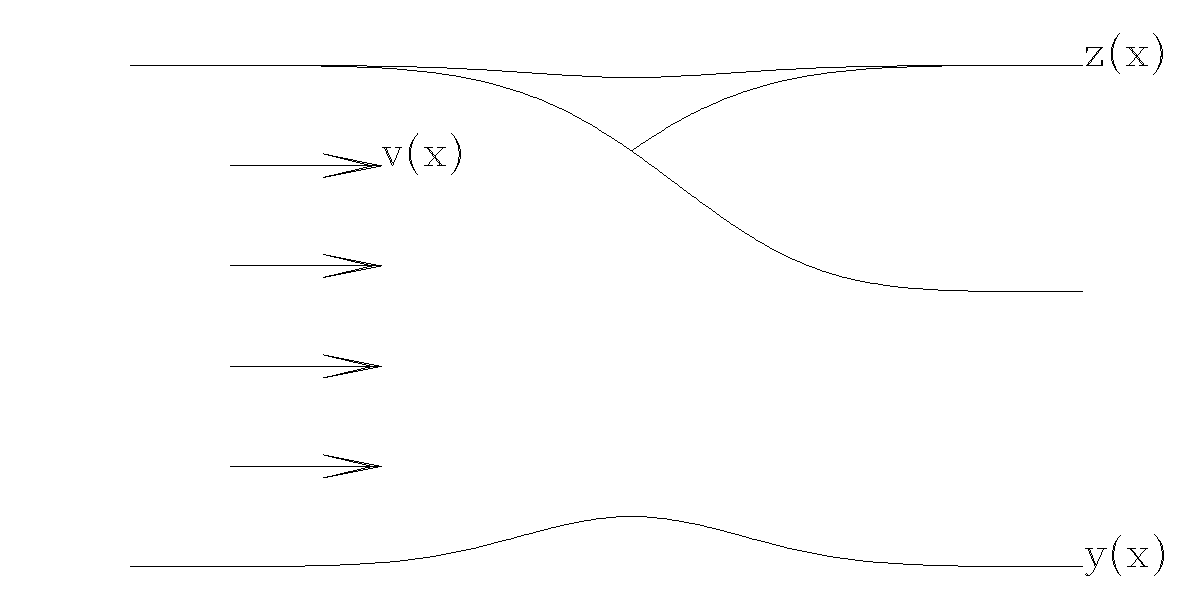
\includegraphics[width=\textwidth]{channel} 
\caption{A channel of variable depth}
\label{fig:channel}
\end{center}
\end{figure}


We can see many of the features of the supersonic flow through a de
Laval nozzle in the flow through a channel.  Much of the intuition
developed in hydraulics carries over to other fluid systems (even
astrophysical ones); furthermore, water running through a channel is
something with which most are familiar.

Let's look at a channel of constant width but varying depth $y(x)$.
Let's take $y$ equals to zero well before the bump.  We would like to
know how the height of the surface of the flow $z(x)$ changes as it
passes through the channel (as shown in Fig.~\ref{fig:channel}).

Let's write out the Bernoulli equation (divided by $g$ as customary in
hydraulics) for the fluid moving along the
surface,
\begin{equation}
\frac{v^2}{2g} + z + \frac{p_a}{g}= \frac{v_0^2}{2g} + z_0 +
\frac{p_a}{g} = h_0
\label{eq:669}
\end{equation}
where $p_a$ is the pressure of the atmosphere.  The quantity $h_0$ is
a constant along the surface streamline, and it is so important in
hydraulics that it has a special name, {\em specific head}.
From continuity we have
\begin{equation}
v \left ( z - y \right ) = v_0 z_0 = q_0
\label{eq:670}
\end{equation}
where $q_0$ is the flux.  Notice that we have neglected
the vertical velocity of the flow.  This is a common assumption in
hydraulics.  Combining the equations yields
\begin{equation}
\frac{v_0^2}{2} \left [ \left ( \frac{z_0}{z-y} \right )^2 - 1 \right
] + g \left (z-z_0\right) = 0 .
\label{eq:bern}
\label{eq:671}
\end{equation}
Taking the derivative with respect to $x$ yields
\begin{equation}
\frac{dy}{dx}=\frac{dz}{dx} \left [ 1 - \frac{g\left(z-y\right)^{3}}{v_0^2
      z_0^2} \right ] = \frac{dz}{dx} \left [ 1 -
    \frac{g\left(z-y\right)}{v^2} \right ] = 
\frac{dz}{dx} \left [ 1 - \mathrm{Fr}^{-2}\right ].
\label{eq:672}
\end{equation}
where $\mathrm{Fr}$ is the Froude number, the ratio of the speed of
flow to the speed of small wavelength gravity waves (see
\S~\ref{sec:gravitywaves}).  We can rearrange this a bit to yield
\begin{equation}
\frac{dz}{dx} = -\frac{dy}{dx} \frac{\mathrm{Fr}^2}{1-\mathrm{Fr}^2},
\label{eq:dzdx}
\label{eq:673}
\end{equation}
so if the fluid is {\em subcritical} or streaming (``subsonic'') over the bump, the surface will dip, and 
if the fluid is {\em supercritical} or shooting (``supersonic'') the surface will bulge.  For the
equation to make sense, if the flow becomes supercritical, it must do
so at the top of the bump.  

Fig.~\ref{fig:channel} shows the various possibilities.  Essentially
for given values of $g, v_0$ and $z_0$ and for a small enough values
of $y(x)$, there are two solutions for $z(x)$.  One is a small
deviation in the level of the surface that corresponds to a subcritical
flow.  The second has a large deviation (supercritical flow).  When the
flow is critical these two solutions coincide.  The upper curves show the
surface for various values of $v_0$.  The uppermost curve is always
well in the subcritical regime.  The middle curve nearly reaches the
critical point at the top of the bump, and the lower curve reaches the
critical point and is supercritical to the right of the bump.

When the flow is critical at the top of the bump, we see that the
smooth solution is the one that goes supercritical after the bump.  At
first glance the whole setup seems quite sensitive.  In particular
what if the bump is so big that the flow goes critical before reaching
the top of the bump?  For a particular set of initial conditions we
can calculate the height of the bump where the fluid goes
critical to be
\begin{equation}
y_c = z_0 + \frac{v_0^2}{2g} - \frac{3 \left (v_0 z_0\right)^{2/3}}{2
  g^{1/3}} = h_0 - \frac{3 q_0^{2/3}}{2 g^{1/3}}
\label{eq:ycrit}
\label{eq:674}
\end{equation}
We can actually do much better than this.  If we look at
Eq.~\ref{eq:bern} and make the substitution $z=y+1/u$ we get
\begin{equation}
\frac{v_0^2 z_0^2}{2} u^3 - \left [ \frac{v_0^2}{2} + g \left ( z_0 -
    y \right )   \right ] u + g = 0.
\label{eq:bernu}
\label{eq:675}
\end{equation}
This equation has the form
\begin{equation}
A u^3 - B u + C = 0.
\label{eq:cubic}
\label{eq:676}
\end{equation}
\index{cubic equation}
Let us substitute $u=\sqrt{4B/3A} \cos t$ to give after some
manipulation
\begin{equation}
\cos 3 t = -\frac{3 C}{2 B} \sqrt{\frac{3A}{B}}
\label{eq:cubic_sol}
\label{eq:677}
\end{equation}
which gives three real solutions for $u$ as long as the absolute value
of the right-hand side does not exceed unity.
We can also use this result to solve for $v_0$ in terms of $y_c$ in
Eq.~\ref{eq:ycrit}.   Both this and the solutions to
Eq.~\ref{eq:bernu} are left for the exercises.


\section{Real Sound Waves}
\label{sec:real-sound-waves}
\index{fluid mechanics!sound waves}
Let's take a closer look at sound waves.  As before we shall assume
that the background is static so before we perturb the medium the
entropy is constant throughout.  Let's perturb the fluid in a
particular wave so that $s$ remains constant.  In this case, we can
express the pressure in terms of the density alone.

Furthermore, let's assume that the velocity of fluid at any point depends
on the density alone and look at the continuity and Euler equations
\begin{equation}
\pp{\rho}{t} + \pp{(\rho v)}{x} = 0, ~~~ \pp{v}{t} + v \pp{v}{x} +
\frac{1}{\rho} \pp{P}{x} = 0
\label{eq:680}
\end{equation}
where we have assumed that the wave is a plane wave travelling in the
$x-$direction.  Using the relationships between the pressure, velocity
and density we can obtain,
\begin{equation}
\pp{\rho}{t} + \dd{(\rho v)}{\rho} \pp{\rho}{x} = 0, ~~~ \pp{v}{t} +
\left ( v + \frac{1}{\rho} \dd{P}{v} \right ) \pp{v}{x} = 0.
\label{eq:681}
\end{equation}
We can define the speed of the wave as the rate at which regions of
the same density or velocity move forward along the $x-$direction,
\begin{equation}
\left( \pp{x}{t} \right )_\rho = - \left [
  \frac{\pp{\rho}{t}}{\pp{\rho}{x}} \right ] = \dd{(\rho v)}{\rho} = v
+ \rho \dd{v}{\rho}
\label{eq:682}
\end{equation}
and
\begin{equation}
\left( \pp{x}{t} \right )_v = - \left [
  \frac{\pp{v}{t}}{\pp{v}{x}} \right ] = v + \frac{1}{\rho} \dd{P}{v}.
\label{eq:683}
\end{equation}
These two velocities must be equal so we get
\begin{equation}
\rho \dd{v}{\rho} = \frac{1}{\rho} \dd{P}{v} = \frac{c_s^2}{\rho} \dd{\rho}{v}
\label{eq:684}
\end{equation}
so
\begin{equation}
v = \pm \int \frac{c_s}{\rho} d\rho = \pm \int \frac{dP}{\rho c_s}.
\label{eq:685}
\end{equation}
We can find how fast a portion of the wave travels by substituting
into Eq.~\ref{eq:684} to get
\begin{equation}
\left( \pp{x}{t} \right )_v = v \pm c_s(v)
\label{eq:686}
\end{equation}
so we find that
\begin{equation}
x = t [  v \pm c_s(v) ] + f(v)
\label{eq:687}
\end{equation}
where $f(v)$ determines the initial shape of the wave.   Let's derive
an expresion for the sound speed as a function of the density,
\begin{equation}
c_s = \left [\dd{P}{\rho}\right ]^{1/2} = \left [ \gamma K
  \rho^{\gamma-1} \right ]^{1/2}
\label{eq:688}
\end{equation}
so
\begin{equation}
\rho = \rho_0 \left ( \frac{c_s}{c_0} \right )^{2/(\gamma-1)}.
\label{eq:689}
\end{equation}
If we substitute this into Eq.~\ref{eq:688} we get
\begin{equation}
c_s = c_0 \pm \frac{1}{2} (\gamma -1 ) v.
\label{eq:690}
\end{equation}
We can use this result to express the density and pressure in terms of
the fluid velocity
\begin{equation}
\rho = \rho_0 \left [ 1 \pm \frac{1}{2} (\gamma-1) \frac{v}{c_0}
  \right]^{2/(\gamma-1)}, ~~~ P = P_0
\left [ 1 \pm \frac{1}{2} (\gamma-1) \frac{v}{c_0}
  \right]^{2\gamma/(\gamma-1)}.
\label{eq:691}
\end{equation}
Putting things together we find that
\begin{equation}
x = t \left [ \pm c_0 + \frac{1}{2} (\gamma+1) v \right ] + f(v)
\label{eq:692}
\end{equation}
or rearranging
\begin{equation}
v = F \left \{ x - \left [ \pm c_0 + \frac{1}{2} (\gamma+1) v \right ]
t \right \}
\label{eq:693}
\end{equation}
If we look at Eq.~\ref{eq:693} we see that we can have a situation where the
same value of $x$ has more than one value of $v$.  This isn't
physical.  This first occurs at a time $t$ when
\begin{equation}
\left ( \pp{x}{v} \right)_t = 0, \left ( \pp{^2x}{v^2} \right)_t = 0, 
\label{eq:694}
\end{equation}
or at
\begin{equation}
t = -\frac{2 f'(v)}{\gamma+1}, f''(v) = 0.
\label{eq:695}
\end{equation}
\index{fluid mechanics!shock formation}
The first expression tells us when the shock forms, and the second
tells us that the shock forms at a point of inflection in the wave.

Another important situation is when the discontinuity forms at a
boundary between gas that is moving at gas that is stationary
($v=0$).  In this case we have
\begin{equation}
t = - \frac{2f'(0)}{\gamma+1}
\label{eq:696}
\end{equation}
As an example let's assume that we have a pipe closed at one end by a
piston and we start to move the piston according to $v_\rmscr{pist}=a
t$.  Because the gas at the edge of the piston must move with the
piston we have $v=at$ at $x=\frac{1}{2} at^2$, so we can write down an
expression for 
\begin{equation}
f(v) = f(at) = \frac{1}{2} at^2 - -c_0 t - \frac{1}{2} (\gamma + 1)
at^2 = -c_0 tb - \frac{1}{2} \gamma at^2 = -\left (\frac{c_0}{a} \right
) v - \frac{1}{2} \frac{\gamma}{a} v^2.
\label{eq:697}
\end{equation}
Using the expression for $x$ we get
\begin{equation}
x - \left [ c_0 + \frac{1}{2} (\gamma+1) v \right ] t = f(v) = -\left (\frac{c_0}{a} \right
) v - \frac{1}{2} \frac{\gamma}{a} v^2.
\label{eq:698}
\end{equation}
Solving for $v$ gives
\begin{equation}
v = \frac{1}{\gamma} \left ( \left \{ \left [ c_0 - \frac{1}{2}
  (\gamma+1) a t \right ]^2 + 2 a \gamma (c_0 t -x ) \right \}^{1/2} -
\left [ c_s - \frac{1}{2} (\gamma + 1 ) a t \right ] \right \}.
\label{eq:699}
\end{equation}
If $a<0$ a rarefaction wave travels through the gas.  On the other
hand if $a>0$ we get a shock at a time,
\begin{equation}
t = - \frac{2 f'(0)}{\gamma+1} = \frac{2 c_0}{a(\gamma+1)}.
\label{eq:700}
\end{equation}
We leave the exploration of shocks to the next chapter; suffice it to
say for now that shocks happen.

\begin{figure}
\begin{center}
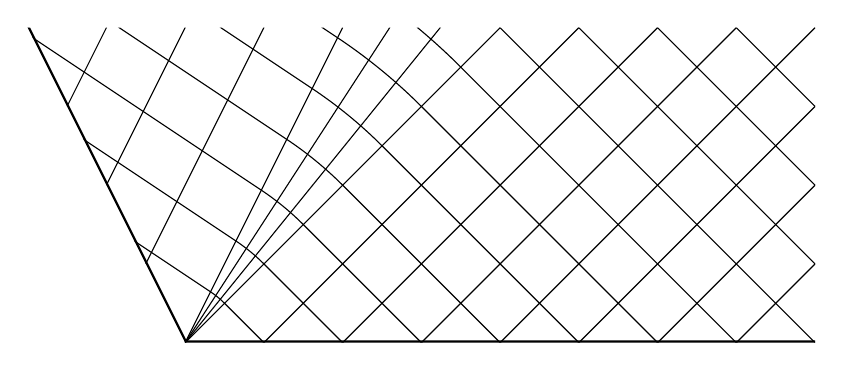
\begin{tikzpicture}
\clip (-2,4) -- (0,0) -- (8,0) -- (8,4) -- cycle;
\draw [ultra thick] (0,0) -- (8,0) (0,0) -- (-2,4);
\foreach \x in {0,...,12} {
  \draw (\x,0) -- ++(4,4) 
%        (\x,0) -- (\x/2,\x/2) arc (45:63.43:0.707*\x) -- ++(-6,4);
        (\x,0) -- (\x/2,\x/2) arc (45:56.3099:1.165*\x) -- ++(-6,4);
}
\foreach \x in {51,57} {
  \draw (0,0) -- (\x:6);
}
\foreach \y in {0,...,4} {
  \draw (-\y/2,\y) -- ++(2,4);
}
\end{tikzpicture}
\end{center}
\caption{The Characteristic Structure for a Rarefaction Wave,
  $a<0$. Notice the smooth transition between the regions.}
\end{figure}

\begin{figure}
\begin{center}
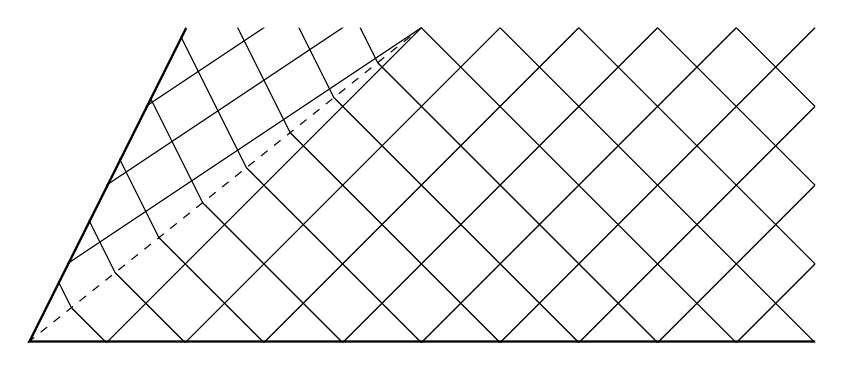
\begin{tikzpicture}
\clip (2,4) -- (0,0) -- (10,0) -- (10,4) -- cycle;
\draw [ultra thick] (0,0) -- (10,0) (0,0) -- (2,4);
\foreach \x in {1,...,14} {
  \draw (\x,0) -- ++(4,4) 
        (\x,0) -- (5*\x/9,4*\x/9) -- ++(-2,4);
}
\draw [dashed] (0,0) -- (5,4);
\foreach \y in {1,...,4} {
  \draw (\y/2,\y) -- ++(6,4);
}
\end{tikzpicture}
\end{center}
\caption{The Characteristic Structure for a Compression Wave, $a>0$. Notice the abrupt transition between the regions.}
\end{figure}

\section{Problems}
\begin{enumerate}


\item{\bf Maximum Flux}

Calculate from the Euler equation and the continuity equation, at what
velocity does the flux ($\rho V$) reach its maximum for fluid flowing 
through a tube of variable cross-sectional area?   
At which velocities does the flux vanish?  You can consider the flow
to be adiabatic.

\item{\bf Stream Bed}

  Fig.~\ref{fig:channel} shows how the level of the surface changes
  for a flow passing over an obstacle.  For an initial depth of
  $z_0=1$ and $g=10$ and a bump height of $y(x)=0.1 e^{-x^2}$, find the
  solutions to Bernoulli's equation (Eq.~\ref{eq:bern}) for $z$ as a
  function of $x$ and the initial velocity $v_0$.  You may find
  several solutions for a given $x$.   Also you should only worry
  about the positive real solutions for $z$.  What are the values of
  the critical velocities $v_0$?

\item{\bf Sound Velocity}

  Show that for a linear sound wave {\em i.e.} one in which $\delta
  \rho \ll \rho$ that the velocity $v$ of fluid motion is much less
  than $c_s$. Estimate the maximum longitudinal fluid velocity in the
  case of a sound wave in air at STP in the case of a disturbance
  which sets up pressure fluctuations of order 0.1\%.
\end{enumerate}


%%% Local Variables:
%%% TeX-master: "book"
%%% End:
\chapter{Shock Waves}
\label{cha:shock-waves}\label{sec:shock-waves}
\index{fluid mechanics!shock waves}
\index{shocks}

\section{Non-relativistic Shocks}
\label{sec:non-relat-shocks}
\index{fluid mechanics!non-relativistic shock waves}
\index{shocks!non-relativistic}

Discontinuities signal a failure of fluid mechanics as we have
formulated it.   Fluid mechanics assumes that the material is
continuous so quantities cannot change discontinuously.  In practice
viscosity and thermal conduction save the day, so although the wave
may get really steep, a discontinuity doesn't actually form.  To
understand the structure of a shock, one needs to include viscosity,
but one can understand the behaviour of shocks without including
viscosity as we shall see.

Let's stand in the frame of the shock.  The fluid approaches the shock
supersonically on the left side and exits subsonically on the right
side.   Let $P_1, \rho_1$ and $v_1$ denote the physical quantities on
the left-hand side (the pre-shock fluid) and $P_2, \rho_2$ and $v_2$
in the post-shock fluid. 

First we have
\begin{equation}
\rho_1 v_1 = \rho_2 v_2 = j.
\label{eq:701}
\end{equation}
What goes into the shock must come out of the shock.  If you remember
the energy flux for an ideal fluid is
\begin{equation}
{\bf q} = \left [ \frac{1}{2} V^2 + w \right ] \rho {\bf V} .
\label{eq:702}
\end{equation}
This flux must be the same on each side (unless the shock is
radiative) so we have
\begin{equation}
\left ( \frac{1}{2} v_1^2 + w_1  \right ) \rho_1 v_1 = 
\left ( \frac{1}{2} v_2^2 + w_2  \right ) \rho_2 v_2 .
\label{eq:703}
\end{equation}
Because of conservation of mass we can simplify this to
\begin{equation}
 \frac{1}{2} v_1^2 + w_1 = \frac{1}{2} v_2^2 + w_2.
\label{eq:704}
\end{equation}
This states that the sum of the kinetic and internal energy per unit
mass is conserved across the shock.   Third we have to conserve the
momentum flux
\begin{equation}
P_1 + \rho_1 v_1^2 = P_2 + \rho_2 v_2^2
\label{eq:705}
\end{equation}
We can use the defintion of the enthalpy to eliminate it from the
equations
\begin{equation}
w = \epsilon + \frac{P}{\rho} = \frac{\gamma}{\gamma-1} \frac{P}{\rho} = 
 \frac{\gamma}{\gamma-1} k_B T.
\end{equation}
Let's define the Mach number of the incoming flow as $M_1=v_1/c_s$ and
rewrite Eq.~\ref{eq:705} as
\begin{equation}
\frac{P_2}{P_1} = 1 + \frac{\rho_1}{P_1} v_1^2 - \frac{\rho_2}{P_1}
v_2^2 = 1 + \gamma M_1^2 \left ( 1 -  \frac{\rho_1}{\rho_2} \right ).
\label{eq:837}
\end{equation}
We can also rewrite Eq.~\ref{eq:704} to yield
\begin{equation}
\frac{P_2}{P_1} = \frac{\rho_2}{\rho_1} + \frac{1}{2} M_1^2 \left
  (\gamma-1\right ) \left( \frac{\rho_2}{\rho_1} -
  \frac{\rho_1}{\rho_2} \right )
\label{eq:842}
\end{equation}
and we can equate these two expressions to solve for $\rho_2/\rho_1$.
From inspection we see that one solution is $\rho_2=\rho_1$, which
means that there is not discontinuity.   The other solution yields
\begin{eqnarray}
\frac{\rho_2}{\rho_1} = \frac{v_1}{v_2} &=& \frac{(\gamma+1) + (\gamma+1)
( M_1^2 - 1 )}{(\gamma+1)+(\gamma-1) (M_1^2-1)} = \frac{(\gamma+1)
  M_1^2}{2 + M_1^2 (\gamma-1)} \label{eq:679}\\
\frac{P_2}{P_1} &=&  \frac{(\gamma+1) + 2\gamma (M_1^2 -
  1)}{(\gamma+1)} = \frac{1-\gamma + 2 M_1^2 \gamma }{(\gamma+1)}, \\
\frac{T_2}{T_1} &=& \frac{(1-\gamma+2 M_1^2 \gamma) [2 + M_1^2
  (\gamma-1)]}{(\gamma+1)^2 M_1^2} \\
M_2^2 &=& \frac{(\gamma+1)+(\gamma-1) (M_1^2-1)}{(\gamma+1) + 2\gamma (M_1^2 -
  1)} = \frac{2+M_1^2(\gamma-1) }{1 - \gamma + 2  M_1^2\gamma}
\label{eq:706}
\end{eqnarray}
where intermediate expressions are given to show that if $M_1>1$, then
$\rho_2>\rho_1$, $P_2>P_1$ and $M_2<1$.
The fluid enters the shock supersonically and leaves the
shock subsonically.  The post-shock fluid has higher pressure and
density.  It is not obvious from the expression but the post-shock
temperature always exceeds the pre-shock value.

As we take the limit of a stong shock $M_1 \rightarrow \infty$ we find
that the compresssion ratio and square of the downstream Mach number approach
\begin{equation}
\frac{\rho_2}{\rho_1} = \frac{\gamma+1}{\gamma-1}~\textrm{and}~M_2^2 = \frac{1}{2} - \frac{1}{2\gamma}.
\label{eq:707}
\end{equation}
For $\gamma=5/3$ the compression ratio is 4 and the downstream Mach
number is $1/\sqrt{5}$.  For a diatomic gas ($\gamma=7/5$) the maximum compression
ratio is larger at 6 and the square of the downstream Mach number is $1/\sqrt{7}$ --- in
fact the compression ratio $\rho_2/\rho_1$ always equals $1/M_2^2 -
1$ for any value of $M_1$.

Although the solution outlined above gives the ratio of pressures,
densities and other quatities as a function of the incoming Mach
number $M_1$, there is an alternative approach that is somewhat more
illustrative.   First let us define the specific volume of the fluid
$V=1/\rho$, so we can write $v_1=jV_1$ and $v_2=jV_2$ from
Eq.~\ref{eq:701}.  Let's substitute this in Eq.~\ref{eq:705} to give
\begin{equation}
p_1 + j^2 V_1 = p_2 + j^2 V_2
\label{eq:844}
\end{equation}
so 
\begin{equation}
j^2 = \frac{p_2-p_1}{V_1-V_2} = - \frac{\Delta p}{\Delta V}.
\label{eq:845}
\end{equation}
Let's use this value of $j^2$ to determine the velocity difference
\begin{equation}
v_1-v_2=j\left ( V_1 - V_2 \right )~\textrm{so}~\left
  (v_1-v_2\right)^2 = \left ( p_2 - p_1 \right ) \left (V_1 -
  V_2\right ) = -\Delta p \Delta V.
\label{eq:848}
\end{equation}
Both Eq.~\ref{eq:845} and~\ref{eq:848}

Now let's use the same values of $v_1$ and $v_2$ in the energy
equation
\begin{equation}
  \label{eq:846}
  w_1 + \frac{1}{2} j^2 V_1^2 = w_2 + \frac{1}{2} j^2 V_2^2
\end{equation}
and
\begin{equation}
  \label{eq:847}
  w_1 - w_2 + \frac{1}{2} \left ( V_1 + V_2 \right ) \left ( p_2 - p_1
  \right ) = 0.
\end{equation}
Because the specific enthalpy $w$ is a function of $P$ and $V$,
Eq.~\ref{eq:847} defines a curve.  Let's specialize for an ideal gas,
for which $w = \gamma/(\gamma - 1) p V$, so 
\begin{equation}
p_2 = p_1 \frac{\frac{\gamma}{\gamma-1} V_1 - \frac{1}{2} \left ( V_1
    + V_2 \right ) }{\frac{\gamma}{\gamma-1} V_2 - \frac{1}{2} \left ( V_1
    + V_2 \right ) }.
\label{eq:851}
\end{equation}
The denominator vanishes for 
\begin{equation}
\frac{V_1}{V_2} = \frac{\rho_2}{\rho_1} = \frac{\gamma+1}{\gamma-1},
\label{eq:852}
\end{equation}
the same value as Eq.~\ref{eq:707}
\begin{figure}
\begin{center}
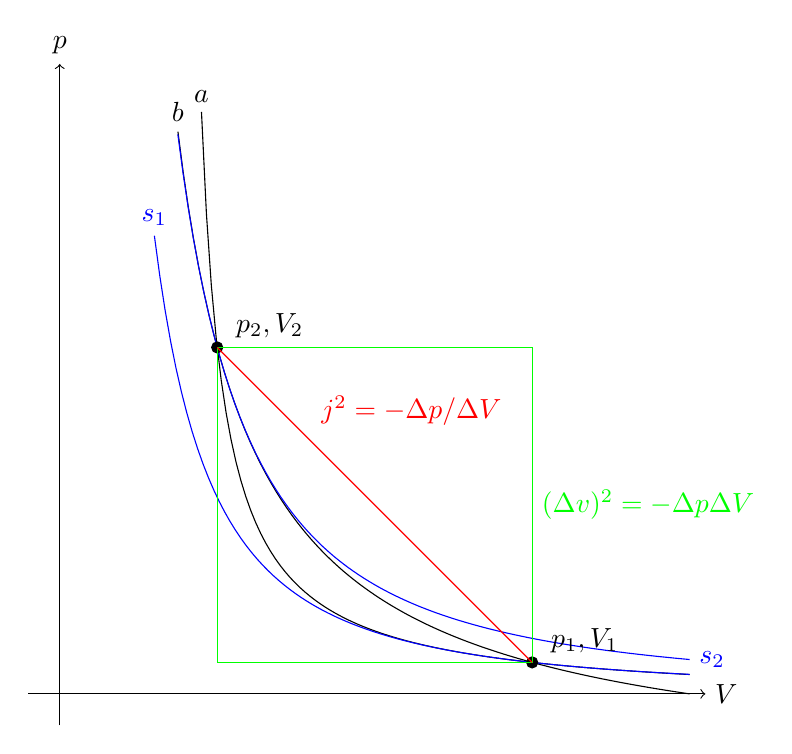
\begin{tikzpicture}
\begin{scope}[xscale=2,yscale=2]
\draw plot [domain=1.33333333:0.3,samples=100] ( 3*\x, { 0.2*(2.5 -
    0.5*(1+\x))/(2.5*\x-0.5*(1+\x))}) node [above] {$a$};
\draw plot [domain=1.33333333:0.25,samples=100] ( 3*\x, { 2.2*(5/6 -
  0.5*(1/3+\x))/(2.5*\x-0.5*(1/3+\x))}) node [above] {$b$};
\draw [blue] plot [domain=1.3333333:0.2,samples=100] ( 3*\x, {
  0.2*exp(-1.666667*ln(\x)) }) node [above] {$s_1$};
\draw [blue] plot [domain=0.25:1.3333333,samples=100] ( 3*\x, {
  2.2*exp(-1.666667*ln(3*\x)) }) node [right] {$s_2$};
\filldraw  (3,0.2) circle (1pt) node [above right] {$~p_1,V_1$}
           (1,2.2) circle (1pt) node [above right] {$~p_2,V_2$};
\draw [green] (3,0.2) rectangle (1,2.2) (3,1.2) node [right] { $(\Delta
  v)^2=-\Delta p \Delta V$};
\draw [red] (3,0.2) -- (1,2.2) (1.6,1.8) node [right] { $j^2 =
  -\Delta p/\Delta V$} ;
\draw [->] (-0.2,0)--(4.1,0) node [right] {$V$} ;
\draw [->] (0,-0.2)--(0,4) node [above] {$p$};
\end{scope}
\end{tikzpicture}
\end{center}
\caption{Shock (Hugoniot) Adiabats (in black) and Standard (Poisson)
  Adiabats (in blue)}
\label{fig:Hugoniot}
\end{figure}
\index{shocks!shock abiabat}
\index{fluid mechanics!Hugoniot abiabat}
\index{Hugoniot abiabat}
Fig.~\ref{fig:Hugoniot} depicts the shock or Hugoniot adiabat for a
shock with a preshock pressure $p_1$ and specific volume $V_1$.  Any
point along the curve $a$ to the left of $(p_1,V_1)$ is a possible
postshock condition.  A particular postshock condition $(p_2,V_2)$ is
highlighted. The minimum flux passing through the shock is
given by the negative of the slope at $(p_1,V_1)$, and it increases as
the shock gets stronger.  The velocity difference vanishes for small
shocks and grows as the area of the box as the shock grows.  

The curve
$b$ to the left of $(p_2,V_2)$ shows the possible postshock conditions
if the preshock condition is $(p_2,V_2)$.  Notice that it also
intersects the curve $a$ at $(p_1,V_1)$.  There are two (or no) shock adiabats
that connect any two points in the $p-V-$plane.  One corresponds to
pressure and density increasing through the shock (curve $a$), and one
corresponds to pressure and density decreasing through the shock
(curve $b$).   Earlier it was stated that these quantities must
increase through the shock, but no reason was given.
Fig.~\ref{fig:Hugoniot} shows the curves of constant entropy
or standard (Poisson) adiabats on the $p-V-$plane corresponding to the
values of the entropy at $(p_1,V_1)$, $s_1$, and  at $(p_2,V_2)$,
$s_2$.   We know that if the pressure is higher at a particular
density or specific volume than the entropy is larger so $s_2>s_1$.
From the second law of thermodynamics we know that entropy cannot
decrease in an isolated system, so the initial state of the flow must
be $(p_1,V_1)$ and the final state is $(p_2,V_2)$.  Furthermore, we
can see that the curves of constant entropy not only pass through the
correponding plots in the plane (this is by design) but they are also
tangent to and have the same radius of curvature as the shock
adiabats.  This means that both the first and second derivatives
coincide for these two sets of curves and that the increase in entropy
is third order in the size of the shock.

Although the curve $b$ that travels from $(p_2,V_2)$ to $(p_1,V_1)$ is
an unphysical solution for a shock because entropy decreases along the
path, it does provide some great insights.  What is the velocity of
the flow on either side of the shock?  We have
\begin{equation}
v_1^2 = j^2 V_1^2 = -\frac{\Delta p}{\Delta V} V_1^2~\textrm{and}~
v_2^2 = -\frac{\Delta p}{\Delta V} V_2^2.
\label{eq:849}
\end{equation}
What is the sound speed on either side of the shock?  We have
\begin{equation}
c_{s,1}^2 = \left . \frac{\partial P}{\partial \rho} \right |_{s_1} =
-V_1^2 \left . \frac{\partial P}{\partial V} \right |_{s_1} = -V_1^2
\left . \frac{\partial P}{\partial V} \right
|_{a}~\textrm{and}~c_{s,2}^2 = -V_1^2
\left . \frac{\partial P}{\partial V} \right |_{b}
\label{eq:850}
\end{equation}
so the Mach numbers on each side of the shock are given by the ratio
of the slope of the secant to the slope of the tangent.  That is,
\begin{equation}
M_1^2 =\frac{\Delta p}{\Delta V} \Big / {\left . \frac{\partial
      P}{\partial V} \right |_{a}}~\textrm{and}~M_2^2 = {
  \frac{\Delta p}{\Delta V} } \Big / {\left . \frac{\partial P}{\partial V} \right |_{b}}.
\end{equation}
Because all of the adiabats are concave up in the $p-V-$plane, the
slope of the secant must be larger than that of the tangent at $(p_1,V_1)$, so
the flow enters the shock supersonically.  Conversely at $(p_2,V_2)$
the slope of the secant must be smaller than that of the tangent, so the
flow exits the shock subsonically.  As the shock decreases in
intensity, the figure demonstrates that both Mach numbers approach
unity.
 

\section{A Spherical Shock - The Sedov Solution}
\label{sec:spher-shock-sedov}
\index{Sedov solution}
\index{fluid mechanics!Sedov solution}
\index{fluid mechanics!spherical shock}

Let's imagine that we dump a really large amount of energy into a
small region.  The energy is initially carried by a small mass ($m$).
Initially, as long as 
\begin{equation}
m \gg \frac{4}{3} \pi r^3 \rho.
\label{eq:708}
\end{equation}
where the right-hand side is the mass swept up.
The ejecta will freely expand.  Let's imagine sometime later when the
mass of the ejecta is negligible but that the energy of the explosion
is still large compared to the enthapy of the swept-up material
\begin{equation}
E \gg \frac{4}{3} \pi r^3 \rho w.
\label{eq:709}
\end{equation}
This is equivalent to $p_2 \gg p_1$, so we have a strong shock, so
$\rho_2/\rho_1 = (\gamma+1)/(\gamma-1)$

In this situation, we only have four numbers of interest,
\begin{itemize}
\item $r$, the distance from the centre of the explosion
\item $t$, the time since the explosion and
\item $E$, the energy of the explosion.
\item $\rho_1$, the density of the undisturbed gas
\end{itemize}
By combining $E$, $t$ and $\rho$ we can find only one expression with
the dimension of length, so let us take the radius of the shock to be
\begin{equation}
R(t) =  R_0 \left ( \frac{E t^2}{\rho_1} \right )^{1/5}.
\label{eq:710}
\end{equation}
where $R_0$ is a dimensionless constant that we will determine from
the solution.  The velocity of the shock wave with respect to the
undisturbed gas is
\begin{equation}
v_s = -v_{1,s} = \dd{R}{t} = \frac{2R}{5t} = \frac{2}{5} R_0 E^{1/5}
\rho_1^{-1/5} t^{-3/5}
\label{eq:711}
\end{equation}
We would like to know the speed of the gas relative to the undisturbed
gas after the shock has passed,
\begin{equation}
v_{2,s} - v_{1,s}  = v_{2,u} - v_{1,u} = v_{2,u}
\label{eq:712}
\end{equation}
For a strong shock we have
\begin{equation}
v_{2,u} = \frac{\gamma-1}{\gamma+1} v_{1,s} - v_{1,s} =
\frac{2}{\gamma+1} v_s
\label{eq:713}
\end{equation}
and
\begin{equation}
\rho_2 = \rho_1 \frac{\gamma+1}{\gamma-1}~\rmmat{and}~P_2 =
\frac{2}{\gamma+1} \rho_1 u_1^2.
\label{eq:714}
\end{equation}
Behind the shock, the fluid is ideal so we can use the continuity,
Euler and energy equations
\begin{eqnarray}
\pp{v}{t} + v \pp{v}{r} +\frac{1}{\rho} \pp{p}{r} &=& 0 \\
\pp{\rho}{t} +  \pp{(\rho v)}{r} + \frac{2\rho v}{r} &=& 0 \\
\left ( \pp{}{t} + v \pp{}{r} \right ) 
\ln \left (\frac{p}{\rho^\gamma} \right ) &=& 0.
\label{eq:715}
\end{eqnarray}
The final equation says that the entropy per unit mass does not
change.
The trick to solve these equations is to assume that all of the
variables depend on the similarity variable $\xi = [ r/R(t) ]$ with
the right scaling.  For example we have
\begin{equation}
v = \frac{2r}{5t} V(\xi), \rho = \rho_1 G(\xi), c_s^2 = \gamma
\frac{P}{\rho} = \frac{4 r^2}{25 t^2} Z(\xi).
\label{eq:716}
\end{equation}
The shock jump conditions give the boundary conditions for the
solution,
\begin{equation}
V(1) = \frac{2}{\gamma+1}, G(1) = \frac{\gamma+1}{\gamma-1}, Z(1) =
\frac{2\gamma (\gamma-1)}{(\gamma+1)^2}.
\label{eq:717}
\end{equation}

Padmanabhan gives a general solution to these equations in closed
form, but let's look at the results for $\gamma=5/3$ depicted in
Fig.~\ref{fig:sedov}.   In general the value of $V$ ranges between $1/\gamma$ at
$\xi=0$ and $2/(\gamma+1)$ at $\xi=1$; it doesn't change much
with the similarity variable; most of the change in the velocity from
the center to the edge comes from the scaling in Eq.~\ref{eq:716}
and the values of $G(\xi)$ and $Z(\xi)$ can be written in terms of
$V(\xi)$.   We can find one of these relationships by examining the
conservation of energy in the flow.  The total energy of the flow is
simply $E$ because no energy leaves the flow and the material swept up
by the shock is assumed to have no energy.  Furthermore, the flow is
self-similar so the energy contained within a spherical shell labelled
by the similarity variable $\xi$ must be constant with time.  Let's
look at a the flow at particular value of $\xi$.  The total energy
flowing outward through a spherical surface over a time $dt$ is 
\begin{equation}
d E = 4\pi r^2 \left ( w+\frac{v^2}{2}\right ) \rho v dt.
\end{equation}
On the other hand the volume swept out
as the flow expands self-similarly is 
\begin{equation}
d V = 4 \pi r^2 \left .\frac{\partial r}{\partial t}\right |_\xi d t.
\end{equation}
We can combine this with the energy density to yield the energy in the region
\begin{equation} 
d E = 4 \pi r^2 \left .\frac{\partial r}{\partial t}\right |_\xi
\left ( \epsilon + \frac{v^2}{2} \right ) \rho d t.
\end{equation}
We can equate these two energies and solve for $c_s^2 = \gamma P/\rho$ to give
\begin{equation}
Z(\xi) = \frac{\gamma(\gamma-1) V(\xi)^2 \left [ 1-V(\xi) \right ]}{2
  \left [ \gamma V(\xi) -1 \right ]}
\end{equation}

The final step in completing the solution is to find the relationship
between the energy of the explosion and the value of $R_0$. We have
\begin{equation}
E = \int_0^R 4 \pi r^2 dr \rho \left [ \frac{v^2}{2} + \epsilon \right
] =\int_0^R 4 \pi r^2 dr \rho \left [ \frac{v^2}{2} +
  \frac{c_s^2}{\gamma(\gamma-1)} \right ]
\end{equation}
and change variables to $\xi$ with $r=R(t) \xi$ to yield
\begin{equation}
E = R(t)^5 \rho_1 \frac{16\pi}{25 t^2} \int_0^1 \xi^4 G(\xi) \left [
  \frac{V(\xi)^2}{2} + \frac{ Z(\xi) }{\gamma(\gamma-1)} \right ] 
\end{equation}
and
\begin{equation}
1 = R_0^5 \frac{16\pi}{25} \int_0^1 \xi^4 G(\xi) \left [
  \frac{V(\xi)^2}{2} + \frac{ Z(\xi) }{\gamma(\gamma-1)} \right ],
\end{equation}
showing explicitly that the value of $R_0$ is a dimensionless number
that only depends on the value of $\gamma$.  The value $R_0$ is
approximately 1.033 for $\gamma=7/5$ and 1.152 for $\gamma=5/3$.  It
ranges from 0.783 to 1.232 as $\gamma$ goes from 1.1 to 1.9.
Amazingly without knowing $\gamma$ well one can get an estimate of the
energy of the blast (within a factor of three) simply from measuring
the value of the radius of the shock at a particular time and taking
$R_0=1$.
\begin{figure}
\begin{center}
\begin{tikzpicture}
\begin{scope}[xscale=5,yscale=3]
\draw plot file{sedov/sedovv.dat} ;
\draw (0.8,0.9) node {$v/v_2$} (0.1,0.4) node {$p/p_2$} (0.3,0.1) node
{$\rho/\rho_2$};
\draw plot file{sedov/sedovrho.dat} ;
\draw plot file{sedov/sedovp.dat} ; 
\draw [->] (-0.2,0)--(1.1,0) node [right] {$r/R$} ;
\draw [->] (0,-0.2)--(0,1.1) ;
\end{scope}
\end{tikzpicture}
\end{center}
\caption{Variation of the density, velocity and pressure behind the
  shock for the Sedov-Taylor blast wave}
\label{fig:sedov}
\end{figure}
% {
% \begin{figure}
% \centering
% \includegraphics[width=\textwidth]{sedov} 
% \caption{Sedov Solution}
% \label{fig:sedov}
% \end{figure}
% }

\section{Detonation Waves}
\label{sec:detonation-waves}
\index{fluid mechanics!detonation waves}

In a detonation as the material passes through the shock energy is
released either through chemical changes or nuclear burning.  One
could have either a release of energy through the shock (like
combustion) or a consumption of energy (like ionization).   The jump
conditions are with the exception of the energy equation
\begin{equation}
\frac{1}{2} v_1^2 + w_1 = \frac{1}{2} v_2^2 + w_2
\label{eq:853}
\end{equation}
where $w_1$ and $w_2$ are now different functions of $p$ and $V$ to
reflect the different chemical or nuclear composition of the gas
before and after the reactions.  Fig.~\ref{fig:Detonation} depicts the
situation graphically.  The lower curve $a$ is the shock adiabat
without the chemical changes and $a'$ is the detonation abiabat which
uses the functional form of the enthalpy in the burnt gas.  We still
have the relationships between the flux, velocities and slopes and
areas on the $p-V-$plane, because these originated from the
conservation of momentum and mass not from the energy equation that
has changed.
\index{shocks!detonation abiabat}
\index{fluid mechanics!detonation abiabat}

The various points outline how the gas changes as it passes through
the shock and burns.  An example of the general case, the gas enters
the shock supersonically at $A$ and is compressed to point $B$ and
leaves the shock subsonically and at the same time or after the gas
burns and moves along the chord to point $E$.  Because the flux of the
flow is conserved through the transition, the state of the gas must
remain on the chord $AB$.  There is a minimum flux that can pass
through the detonation front, $j_\mathrm{min}$, and this flux also
corresponds to the minimum velocity jump through the front where the
final state is $O$ or the Jouguet point.  In the
case of a shock without a chemical change there is no minimum velocity
jump.  

\index{Jouguet point}
\index{shocks!Jouguet point}
\index{Chapman-Jouguet condition}
Although the minimal value of the flux appears to be a special case,
it is actually occurs in nature often.  A detonation that proceeds
from $A$ to $D$ and then to $O$ minimizes the entropy incease in the
front. Furthermore, for final states above $O$ along $a'$ the gas
leaves the front subsonically.  If the final state lies at $O$, the
gas leaves the detonation front right at the speed of sound in the
downstream flow.  This special situation often arises when the
combustion itself creates the shock.  Let's take a specific example of
a detonation front that starts near the closed end of a tube.  The
front must be followed by a rarefaction wave that travels up the tube
at the speed of sound through the postshock gas.  If the postshock gas
is traveling subsonically relatively to the shock then the rarefaction
wave will eventually catch up to the back of the shock reducing the
flux through the shock by reducing the postshock pressure and shock
velocity relative to the preshock gas until the minimum flux is
achieved.  At this point the postshock gas leaves the front at the
sound speed so the rarefaction wave no longer overtakes the shock and
the combined detonation front and rarefaction wave achieves a steady
state.  The detonation adiabat below the Jouguet point $O$ cannot be
reached if the combustion begins after the gas is compressed.  The
point $E$ for example has a lower entropy than point $C$ so the gas
cannot pass from $C$ to $E$ either immediately after the shock or
through a subsequent shock.

% $\beta P_1/\rho_1$ is the energy per unit mass released or
% removed as material passes through the shock.  In this case
% Eq.~\ref{eq:837} stands but Eq.~\ref{eq:842} becomes
% \begin{equation}
% \frac{P_2}{P_1} = \frac{\rho_2}{\rho_1} \left ( 1 - \beta
%   \frac{\gamma-1}{\gamma} \right ) + \frac{1}{2} M_1^2 \left
%   (\gamma-1\right ) \left( \frac{\rho_2}{\rho_1} -
%   \frac{\rho_1}{\rho_2} \right ).
% \label{eq:843}
% \end{equation}
% It is apparent that we still have two solutions but $\rho_2=\rho_1$ is
% not one of them.

\begin{figure}
\begin{center}
\begin{tikzpicture}
\begin{scope}[xscale=2,yscale=2]
\draw [gray] plot [domain=1.33333333:0.3,samples=100] ( 3*\x, { 0.2*(2.5 -
    0.5*(1+\x))/(2.5*\x-0.5*(1+\x))}) node [above] {$a$};
\draw plot [domain=1.33333333:0.345,samples=100] ( 3*\x, { 0.4*(2.5 -
    0.5*(1+\x))/(2.5*\x-0.5*(1+\x))}) node [above] {$a'$};
% \draw [blue] plot [domain=1.3333333:0.2,samples=100] ( 3*\x, {
%   0.2*exp(-1.666667*ln(\x)) }) node [above] {$s_1$};
% \draw [blue] plot [domain=1.3333333:0.2,samples=100] ( 3*\x, {
%   0.4*exp(-1.666667*ln(\x)) }) node [above] {$s_1'$};
% \draw [blue] plot [domain=0.25:1.3333333,samples=100] ( 3*\x, {
%   2.2*exp(-1.666667*ln(3*\x)) }) node [right] {$s_2$};
\draw [blue] plot [domain=0.8:4,samples=100] ( \x, {
  0.7075383629*exp(-1.666667*ln(\x/2.1383708395)) }) node [right] {$s_O$};
\filldraw  (3,0.2) circle (1pt) node [ below left] {$A$} 
           (1,2.2) circle (1pt) node [above right] {$B$}
           (1.315,1.885) circle (1pt) node [above right] {$C$}
           (2.73,0.47) circle (1pt) node [above right] {$E$}
           (3, 0.2) ++(149.5:2.12) circle (1pt) node [above right] {$D$}
           (3, 0.2) ++(149.5:1) circle (1pt) node [below] {$O$};
% \draw [green] (3,0.2) rectangle (1,2.2) (3,1.2) node [right] {
% $(\Delta v)^2=-\Delta p \Delta V$};
\draw [red,dashed] (3,0.2) -- (1,2.2) (1.6,1.8) node [right] { $j^2 =
  -\Delta p/\Delta V$} ;
\draw [red] (3,0.2) -- ++(149.5:2.12) (2,0.8) node [left] { $j_\mathrm{min}^2$ };
\draw [->] (-0.2,0)--(4.1,0) node [right] {$V$} ;
\draw [->] (0,-0.2)--(0,4) node [above] {$p$};
\end{scope}
\end{tikzpicture}
\end{center}
\caption{Shock (Hugoniot) Adiabat (in gray), Detonation Adiabat (in
  black) and Standard (Poisson) Adiabat (in blue)}
\label{fig:Detonation}
\end{figure}

\section{Radiative Shocks}
\label{sec:radiative-shocks}
\index{fluid mechanics!radiative shocks}
\index{shocks!radiative}

So far we have assumed that the energy in a fluid element is conserved
through the shock, that no energy leaves the flow or is radiated.  The
opposite extreme is that the shock heats the gas sufficiently that
radiative losses are important near the shock and the gas rapidly
cools.  In this case we must abandon the conservation of energy flux
through the shock (Eq.~\ref{eq:704}) and find another criterion to
understand how the gas changes through the shock.  Astrophysically the
rate that gas cools can depend very sensitively on the temperature of
the gas.  In particular gas above about $10^4$~K radiates much more
effectively than cooler gas.  Imagine if the gas before the shock was
just below the critical temperature at which cooling set in.  As it
passes through the shock, it goes above this temperature and then
rapidly begins to cool and rapidly returns to its initial
temperature.  The additional condition that we seek is that final
temperature equals the initial temperature.
\index{shocks!isothermal}
\index{fluid mechanics!isothermal shocks}
\begin{figure}
\begin{center}
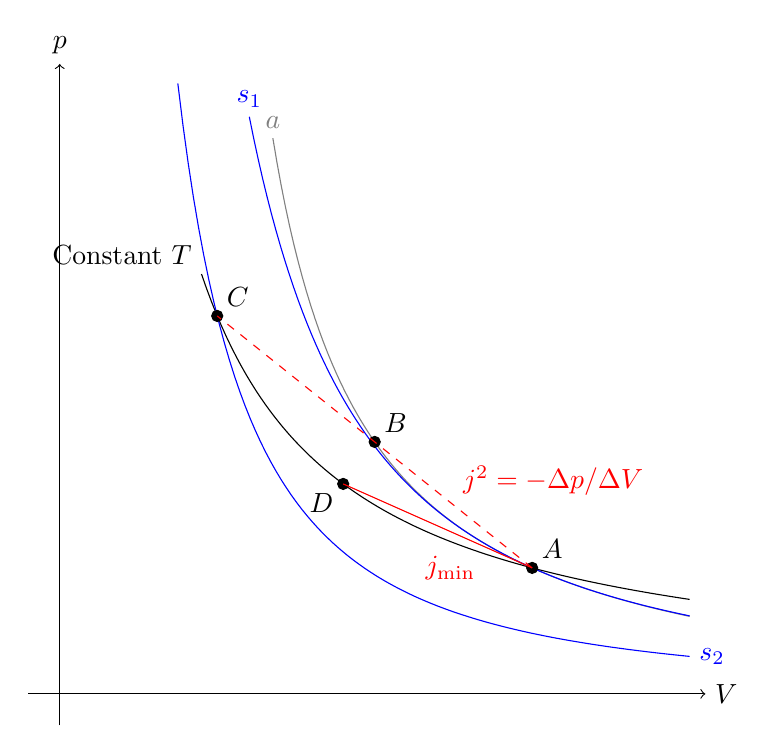
\begin{tikzpicture}
\begin{scope}[scale=2]
\draw [gray] plot [domain=1.33333333:0.45,samples=100] ( 3*\x, { 0.8*(2.5 -
    0.5*(1+\x))/(2.5*\x-0.5*(1+\x))}) node [above] {$a$};
\draw plot [domain=1.33333333:0.3,samples=100] ( 3*\x, { 0.8/\x}) node
[above left] {Constant $T$};
\draw [blue] plot [domain=1.3333333:0.4,samples=100] ( 3*\x, {
  0.8*exp(-1.666667*ln(\x)) }) node [above] {$s_1$};
\draw [blue] plot [domain=0.25:1.3333333,samples=100] ( 3*\x, {
  2.4*exp(-1.666667*ln(3*\x)) }) node [right] {$s_2$};
\filldraw  (3,0.8) circle (1pt) node [above right] {$A$}
           (2,1.6) circle (1pt) node [above right] {$B$}
           (1,2.4) circle (1pt) node [above right] {$C$}
           (1.8,1.3333333) circle (1pt) node [below left] {$D$};
\draw [dashed,red] (3,0.8) -- (1,2.4) node [pos=0.25, above right] { $j^2 =
  -\Delta p/\Delta V$} ;
\draw [red] (3,0.8) -- (1.8,1.3333333) node [pos=0.25, below left] {
  $j_\mathrm{min}$ } ;
\draw [->] (-0.2,0)--(4.1,0) node [right] {$V$} ;
\draw [->] (0,-0.2)--(0,4) node [above] {$p$};
\end{scope}
\end{tikzpicture}
\end{center}
\caption{Isotherm (in black), Shock (Hugoniot) Adiabat (in gray), Standard (Poisson)
  Adiabats (in blue)}
\label{fig:isothermalshock}
\end{figure}

Again we still have the relationships between the flux, velocities,
slopes and areas on the $p-V-$plane that result from the conservation
of momentum and mass, but the shock adiabat is replaced with an
isotherm as shown in Fig.~\ref{fig:isothermalshock}.  From the diagram
it is apparent that the entropy of the gas decreases through an
isothermal shock; as a gas is compressed at constant temperature, its
entropy decreases.  The radiation carries away both energy and
entropy.  Because the standard adiabats are generally steeper than the
isotherms, the gas always leaves the shock subsonically.  Again
because the momentum flux is conserved, the gas must remain on the
chord $AC$ throughout.   As it passed through the shock it is heated
from $A$ to point $B$ and then as it cools it travels from $B$ to $C$.
As for the case of a detonation, we find that there is a minimum flux
that can pass through an isothermal shock and a minimal velocity
change.  Just above the flux $j_\mathrm{min}$ the flow enters the
shock slightly supersonically and leaves subsonically.

The initial and final Mach numbers and densities are related through
\begin{equation}
M_2 = \frac{1}{\gamma M_1}, \frac{\rho_2}{\rho_1} = \gamma M_1^2, \frac{P_2}{P_1} = \gamma M_1^2.
\label{eq:678}
\end{equation}
The ratio of the energy flux entering the radiative shock to that
leaving is given by
\begin{equation}
\frac{q_1}{q_2} = \gamma^2 M_1^2 \frac{(\gamma-1) M_1^2 + 2}{2 \gamma^2
  M_1^2 + \gamma - 1}.
\end{equation}
For large values of $M_1$ the initial energy flux is much larger than
the final energy flux.  At the other end the minimum value of $M_1$ is
of course unity. This yields a minimum energy ratio for the isothermal
shock of
\begin{equation}
\left .  \frac{q_1}{q_2} \right |_\mathrm{min} = \frac{\gamma^2}{2
  \gamma -1}.
\end{equation}
Even this weakest of isothermal shocks results in a compression ratio
$\rho_2/\rho_1 = \gamma$.

Sometimes the temperature of the gas is held constant through the
interaction with an external radiation field, so that even slight
departures from isothermality disappear on a short timescale.  In this
case it makes sense to take $\gamma=1$.   If we substitute $\gamma=1$
in Eq.~\ref{eq:679} through~\ref{eq:706} we obtain Eq.~\ref{eq:678}.
However, the enthalpy of an isothermal gas is given by
\begin{equation}
  w = c_s^2 \ln \left ( \frac{\rho}{\rho_0} \right ),
\end{equation}
so if we take the reference density $\rho_0=\rho_1$ we find
\begin{equation}
\frac{q_1}{q_2} = \frac{M_1^4}{1+\ln M_1^4}
\label{eq:757}
\end{equation}

\section{Relativistic Shocks}
\label{sec:relativistic-shocks}
\index{fluid mechanics!relativistic shock waves}
\index{shocks!relativistic}

We will look at relativistic shocks as an example of relativistic
hydrodynamics.  In particular we will look at the relativistic jump
conditions across the shock.  The particle flux must be conserved
across the shock (Eq.~\ref{eq:616})
\begin{equation}
J_{x,1} = J_{x,2}, \frac{U_1}{V_1} = \frac{U_2}{V_2}
\label{eq:854}
\end{equation}
where $V_1=1/n_{\mathrm{prop},1}$ and $U_1 = \gamma_1 v_1/c$
is the spatial component of four-velocity of the flow before the shock
and $\gamma_1=(1-v_1^2/c^2)^{-1/2}$.  It is most clear to use the
rest-mass energy density for $n_\mathrm{prop}$.  The components of the
stress-energy tensor must also be conserved (Eq.~\ref{eq:627})
\begin{equation}
T_{x0,1}=T_{x0,2}, w_1 U_1 \gamma_1= w_2 U_2 \gamma_2
\label{eq:855}
\end{equation}
and
\begin{equation}
T_{xx,1}=T_{xx,2}, w_1 U_1^2 + p_1 = w_2 U_2^2 + p_2
\label{eq:856}
\end{equation}
where $w=\epsilon + p$ and $\epsilon$ includes the rest-mass energy of
the particles.  Here $w$ is the enthalpy per unit volume whereas in
previous sections it denoted the enthalpy per unit mass,
$w_\mathrm{mass}=w_\mathrm{volume} V$.

By combining the particle flux, Eq.\ref{eq:854}, and the momentum
equations, Eq.~\ref{eq:856}, we obtain the results
\begin{eqnarray}
j^2 &=& \frac{p_2-p_1}{w_1 V_1^2 - w_2 V_2^2} = \frac{p_2-p_1}{V_{w,1} - V_{w,2}}, 
\label{eq:859}
\\
\left( U_1 - U_2 \right )^2 &=&
j^2 \left( V_1 - V_2 \right )^2  =  \frac{V_1-V_2} {V_{w,1}-V_{w,2}}
\left (p_2 - p_1 \right ) \left ( V_1 - V_2 \right )
\label{eq:857}
\end{eqnarray}
where $V_w = w V^2=(p + \epsilon ) V^2$.  These are analogous to
Eq.~\ref{eq:845} and~\ref{eq:848}.  Finally we can derive the equation
of the shock adiabat, using the identity $\gamma^2 = 1 + U^2$, to
yield
\begin{equation}
  w_1 V_{w,1} - w_2 V_{w.2} + \left( V_{w,1} + V_{w,2} \right ) \left (p_2 - p_1 \right ) = 0
\label{eq:860}
\end{equation}
which is very close in form to Eq.~\ref{eq:847}.  In the
non-relativistic limit for the second term we can take $V_w=V$,
but we must look at the first terms more closely because the result
depends on the difference of two quantities that are equal to lowest
order in the non-relativistic limit.  In particular,
\begin{equation}
w_1 V_{w,1} = w_1^2 V_1^2 = \left ( \rho_1 c^2 + w_{NR,1} \right )^2
V_1^2 = 1 + 2 w_{NR,1} V_1 + w_{NR,1}^2 V_1^2
\label{eq:861}
\end{equation}
where we have used $\rho_1 c^2 V_1=1$.  We can drop the last term.
The first term cancels in Eq.~\ref{eq:860}, leaving the middle term
which equals twice the enthalpy per unit mass and results in
twice Eq.~\ref{eq:847}.

\section{Hydraulic Jump}
\label{sec:hydraulic-jump}
\index{fluid mechanics!hydraulic jump}
\index{shocks!hydraulic jump}
Let's revist the dynamics of water travelling down a shallow channel.
We neglect the vertical motion of the fluid and assume that all
dimensions are large compared with the depth of the fluid --- this is the
{\em hydraulic} approximation.  If the flow only depends on the
position $x$ along the channel and time $t$, the continuity and
momentum equation are
\begin{equation}
\pp{h}{t} + \pp{(vh)}{x} = 0, \pp{v}{t} + v \pp{v}{x} = -g \pp{h}{x}.
\label{eq:862}
\end{equation}
where the depth $h$ is assumed to be constant across the channel.  We
can define a surface density ${\bar \rho} = \rho h$ and a mean
pressure ${\bar p}=\rho g h^2/2$ and recast the equations as
\begin{equation}
\pp{\bar \rho}{t} + \pp{(v {\bar \rho}}{x} = 0, \pp{v}{t} + v \pp{v}{x} =
-\frac{1}{\bar \rho} \pp{\bar p}{x}.
\label{eq:862}
\end{equation}
These equations are identical to the equations for the adiabatic flow
of a gas with $\bar p \propto \bar \rho^2$.  We can apply the results
from gas dynamics to hydraulics as along as the flow is abiabatic ---
no shocks.

These equations do not include the conservation of energy equation
because we assume that the flow does not have any internal energy or
entropy.  In practice the energy in the flow can be transferred to
small scale motion of the fluid which is quickly dissipated.  Let us
examine discontinuities in the fluid height and velocity by using the
conditions of continuity on the particle and momentum flux.  Such
discontinuities are known as {\em hydraulic jumps}. The mass
flux density is simply $j=\rho v h$ and the momentum flux is
\begin{equation}
\int_0^h \left ( p + \rho v^2 \right ) dz = \frac{1}{2} \rho g h^2 +
\rho v^2 h.
\label{eq:863}
\end{equation}
The jump conditions are 
\begin{equation}
v_1 h_1 = v_2 h_2, v_1^2 h_1 + \frac{1}{2} g h_1^2= v_2^2 h_2 + \frac{1}{2} g h_2^2.
\label{eq:864}
\end{equation}
We can express any two quantities in terms of the others in particular
we have the velocities in terms of the heights
\begin{equation}
v_1^2 = \frac{1}{2} g \frac{h_2}{h_1} \left ( h_1 + h_2 \right ),
v_2^2 = \frac{1}{2} g \frac{h_1}{h_2} \left ( h_1 + h_2 \right ).
\label{eq:865}
\end{equation}
If we look at the energy flux in the channel we have
\begin{equation}
q = \int_0^h \left ( \frac{p}{\rho} + \frac{1}{2}v^2 \right ) \rho v
dz = \frac{1}{2} j \left ( g h + v^2 \right ) 
\label{eq:866}
\end{equation}
and the difference in energy flux is
\begin{equation}
q_1 - q_2 = g j \frac{\left (h_1^2 + h_2^2 \right ) (h_2 - h_1)}{4 h_1
  h_2}. 
\label{eq:867}
\end{equation}
Because the energy flux of the flow must decrease through the jump
$h_2>h_1$ --- the height of the fluid must increase downstream of the
jump.  Substituting $h_2<h_1$ into Eq.~\ref{eq:865} shows that $v_1 .
\sqrt{g h_1}$ and $v_2 > \sqrt{g h_2}$.  The flow enters the jump
supercritically and leaves the jump subcritically.

\section{Problems}
\begin{enumerate}

\item{\bf Shock Entropy}
  Show that the entropy of the fluid increases as it passes
  through a shock. Hint: the equation of state of an isentropic fluid
  is $P = K\rho^\gamma$ where the value of $K$ increases with
  increasing entropy.

\begin{figure}
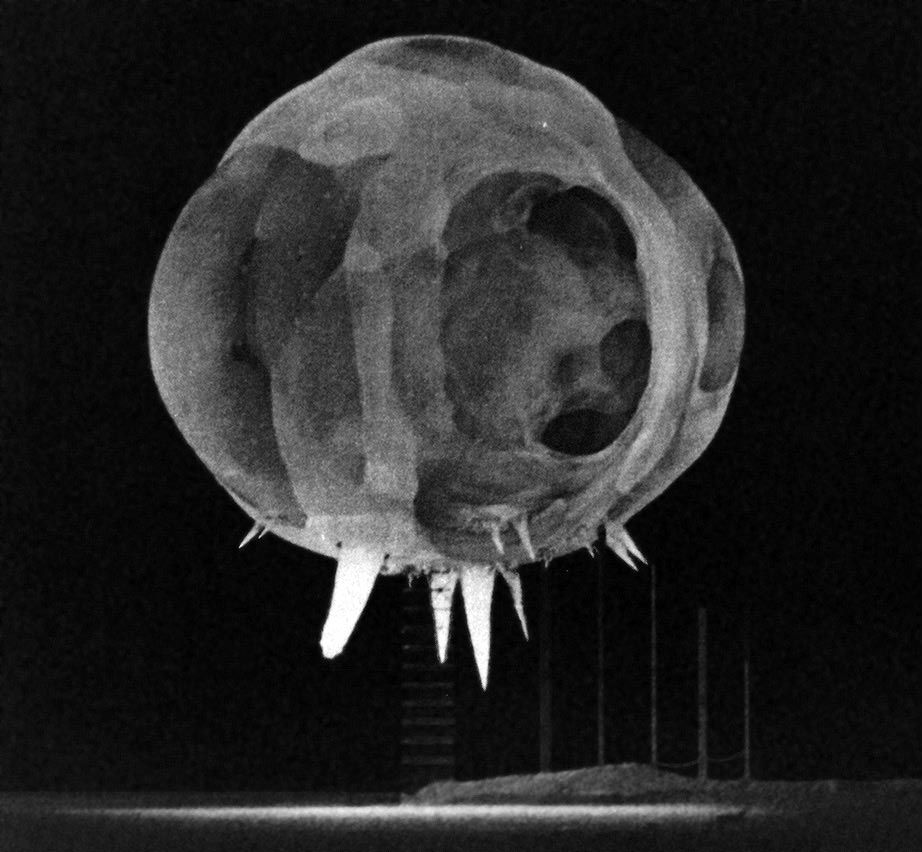
\includegraphics[width=\textwidth]{Tumbler_Snapper_rope_tricks.jpg}  
\caption{The explosion of nuclear device in 1952 about 2~ms after detonation.}
\label{fig:tumbler}
\end{figure}

\item{\bf Bomb Yield}

  Fig.~\ref{fig:tumbler} shows shocked air heated to incandescence
  about two milliseconds after the detonation of a nuclear
  bomb.  The height of the device was 90~meters.  What
  was the approximate yield of the device?

\item{\bf Relativistic Shock}

  Find the incoming and outgoing velocity of a relativistic shock in
  terms of the energy density and pressure on either side of the
  shock.

\item{\bf Relativistic Bernoulli}

  Find the relativistic generalisation of Bernoulli's equation for a
  streamline (you can neglect gravitiy).

\item{\bf Bathtub Physics}

  When water flows into a bathtub, a circular hydraulic jump forms
  around the incoming stream of water.  If you assume that the flow
  rate is constant and the flow is initially vertical, calculate the
  height of the water downstream of the jump as a function of the
  radius of the jump and the flow rate.  You may neglect friction and
  assume that the velocity upstream of the jump is constant. If
  the bathtub is large compared to the radius of the jump and the
  walls are vertical, how does the radius of the jump change with
  time?
\end{enumerate}
%%% Local Variables:
%%% TeX-master: "book"
%%% End:

\chapter{Accretion and Winds}
\label{cha:accretion-winds}
We continue looking at steady flows with two specific applications:
matter flowing onto an object (accretion) and matter flowing away from
an object (winds). 

\section{Spherical Accretion}
\label{sec:spherical-accretion}
\index{fluid mechanics!spherical accretion}
\index{spherical accretion}
We can apply what we learned about the de Laval nozzle to accretion
onto an astrophysical object.  We will assume that the accretion is
steady at a rate ${\dot M}$ and that the pressure $P \propto
\rho^\gamma$ with $1 < \gamma < 5/3$.   First let's write the
continuity equation
\begin{equation}
\frac{1}{r^2} \pp{}{r} \left ( r^2 \rho v \right ) = 0 
\label{eq:718}
\end{equation}
so $\rho v r^2=$constant.  Let's write down the Euler equation
\begin{equation}
v\pp{v}{r} + \frac{1}{\rho} \pp{p}{r} + \frac{GM}{r^2} = 0
\label{eq:719}
\end{equation}
Let's use the equation of state to eliminate $p$ from the Euler
equation and use the continuity equation to eliminate $\rho$,
\begin{equation}
\frac{1}{\rho} \pp{\rho}{r} = -\frac{1}{vr^2}
\pp{}{r}(vr^2)~\rmmat{and}~\pp{p}{r} = \pp{p}{\rho} \pp{\rho}{r} =
c_s^2 \pp{\rho}{r},
\label{eq:720}
\end{equation}
we get
\begin{equation}
v\pp{v}{r} - \frac{c_s^2}{vr^2} \pp{}{r} (vr^2) + \frac{GM}{r^2} = 0.
\label{eq:721}
\end{equation}
We can rearrange this 
\begin{equation}
\frac{1}{2} \left ( 1 - \frac{c_s^2}{v^2} \right ) \pp{v^2}{r} =
-\frac{GM}{r^2} \left ( 1 - \frac{2c_s^2 r}{GM} \right ).
\label{eq:722}
\end{equation}
Far away from the star, the sound speed $c_s$ approaches some constant
value, so the right hand side of the equation will be positive at
large $r$.  We would like the gas to accelerate toward the star, so
$\pp{v^2}{r} < 0$ at large distances.  For this to be the case $v<c_s$
far from the star.   As the gas falls toward the star, it accelerates
until it reaches the critical radius.
\begin{equation}
\frac{2c_s^2 r_c}{GM} = 1
\ee 
If we use $c_s^2 = \gamma p/\rho=\gamma k T$ we get
\begin{equation}
r_c = \frac{GM}{2c_s^2(r_c)} \approx 7.5 \times 10^{13} \left (
\frac{T}{10^4 K} \right )^{-1} \left ( \frac{M}{\rmmat{M}_\odot}
\right )\rmmat{cm} 
\label{eq:723}
\end{equation}
that is much larger that most stars, so we have to worry about what
happens with $r_c$.  If the flow is subsonic when it gets to $r_c$ it
will decelerate within $r_c$ and the accretion stagnates.  If the flow
becomes supersonic before reaching $r_c$, then $\pp{v^2}{r}$ diverges
as the flow becomes supersonic.  This is unphysical because you get
two values of $v^2$ at a single value of $r$.

The only viable accretion mode is for the flow to become supersonic
precisely at $r_c$.  It then accelerates for $r<r_c$ as well.  We can
work further to determine the flow by integrating Eq.~\ref{eq:719} to get a
Bernoulli equation
\begin{equation}
\frac{v^2}{2} + \frac{c_s^2}{\gamma - 1} - \frac{G M}{r} = \rmmat{constant}
\label{eq:724}
\end{equation}
We know that as $r \rightarrow \infty$, $v^2 \rightarrow 0$ so we have
\begin{equation}
\frac{v^2}{2} + \frac{c_s^2 - c_s^2(\infty)}{\gamma - 1} - \frac{G M}{r} = 0.
\label{eq:725}
\end{equation}
At the critical radius we have $v^2=c_s^2$ and $GM/r_c = 2 c_s^2$, so
\begin{equation}
\frac{c_s^2(r_c)}{2} + \frac{c_s^2(r_c) - c_s^2(\infty)}{\gamma-1} - 2
c_s^2(r_c) = 0 .
\label{eq:726}
\end{equation}
We can find that
\begin{equation}
c_s^2(r_c) = c_s^2(\infty) \left [ \frac{2}{5 - 3 \gamma } \right ]
\label{eq:727}
\end{equation}
so
\begin{equation}
r_c = \frac{G M}{c_s^2(\infty)} \frac{5 - 3 \gamma}{4}
\label{eq:728}
\end{equation}
and
\begin{equation}
\rho (r_c) = \rho(\infty) \left [ \frac{2}{5-3\gamma} \right ]^{1/(\gamma-1)}
\label{eq:729}
\end{equation}
We can determine 
\begin{eqnarray}
{\dot M} &=& 4\pi r_c^2 \rho(r_c) c_s(r_c) = \pi G^2 M^2
\frac{\rho(\infty)}{c_s^3(\infty)} \left(  \frac{2}{5-3\gamma} \right
)^{(5-3\gamma)/2(\gamma-1)} \\
&=& 1.4 \times 10^{11}\rmmat{g s}^{-1} \left
(\frac{M}{\rmmat{M}_\odot} \right )^2 \left [
  \frac{\rho(\infty)}{10^{-24} \rmmat{g cm}^{-3}} \right ] \left [
  \frac{c_s(\infty)}{10 \rmmat{km s}^{-1}} \right ]^{-3}.
\label{eq:730}
\end{eqnarray}
for $\gamma=1.4$.  The gamma-dependent factor ranges from $e^{3/2}$
for $\gamma=1$, to $5/2$ at $\gamma=7/5$ and 1 at $\gamma=5/3$.
{
\begin{figure}
\centering
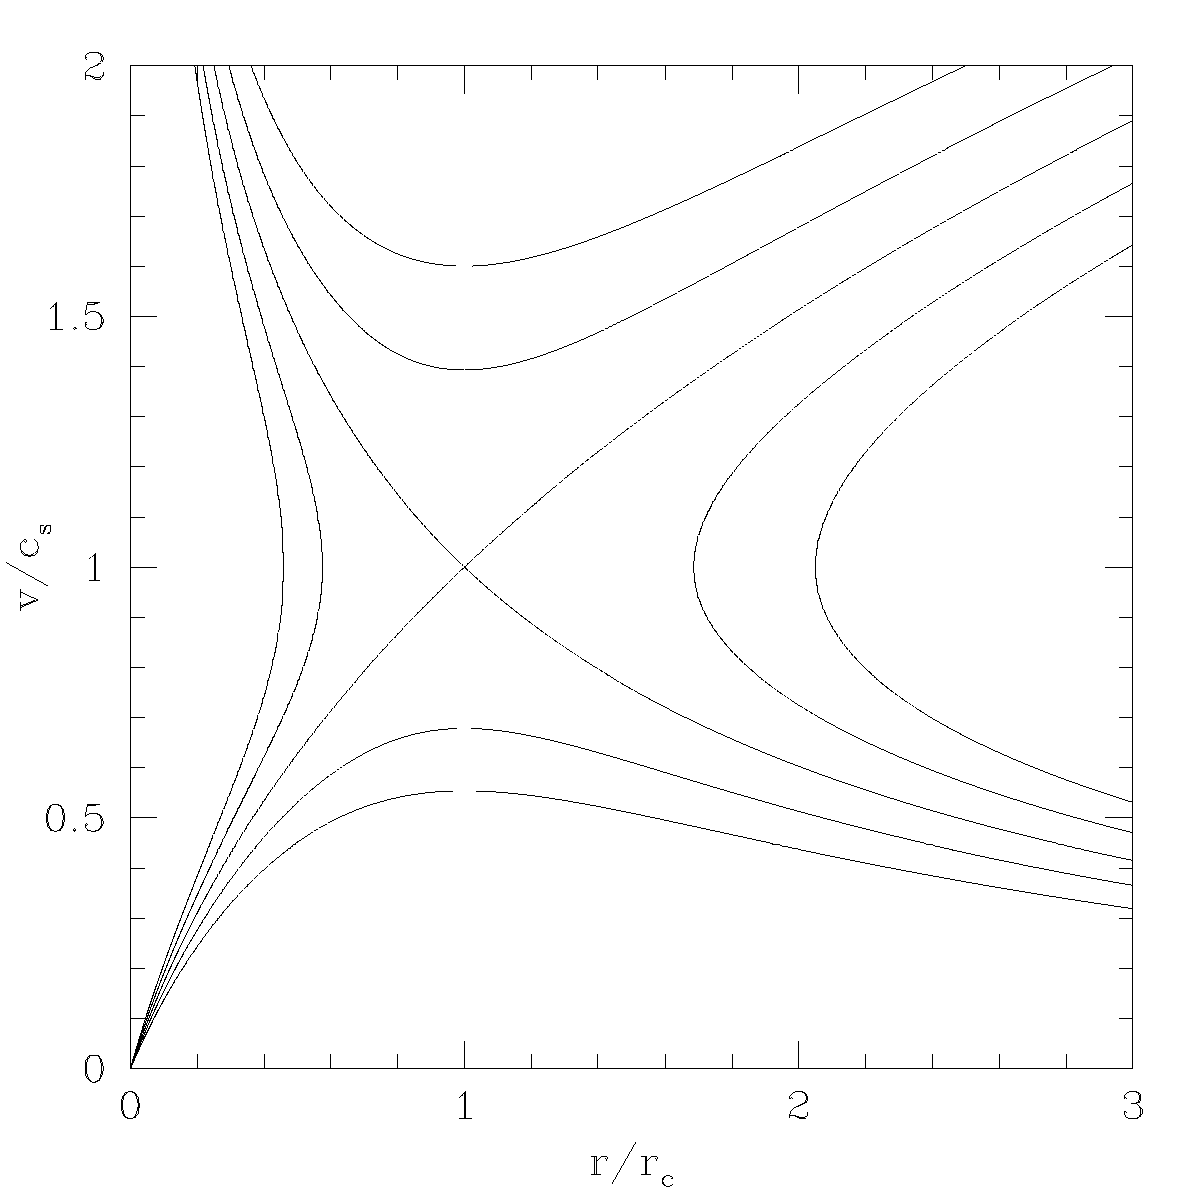
\includegraphics[width=\textwidth]{bondijsh} 
\caption{The solution to Bondi accretion with $\gamma=7/5$ (an
  adiabatic, diatomic gas).}
\label{fig:bondi}
\end{figure}
}

\section{Accretion Disks}
\index{fluid mechanics!accretion disks}
\index{accretion disks}

The preceding section ignores an important aspect of accretion: the
angular momentum of the accreta.  If the material starts with some net
angular momentum it can only collapse so far before its angular
velocity will be sufficient to halt further collapse.  For the
accetion to proceed, angular momentum must be transferred outwards
through the accreted material or removed from the central regions with
ejecta.  Understanding the production of ejecta is beyond our scope, but
examining the transport of angular momentum through a rotating disk of
material is not once we add an additional ingredient to our analysis, 
viscosity.

First let's see why angular momentum can play a crucial role in
accretion.  If we assume that the material had some initial velocity
$v$ relative to the star, and that without gravity it would come
within a distance $b$ of the star (the impact parameter).  The initial
specific angular momentum is $v b$.  If the material conserves angular
momentum we can compare the centripetal acceleration with
gravitational acceleration to give
\begin{equation}
\frac{\left (v b\right)^2}{r^3} = \frac{GM}{r^2},
\label{eq:731}
\end{equation}
so the accretion will stall at
\begin{equation}
r = \frac{\left (v b\right)^2}{GM} = 10^{-3} \mathrm{AU} 
\left (\frac{v}{1\mathrm{km/s}} \frac{b}{1\rmmat{AU}}\right)^2 \frac{\mathrm{M}_\odot}{M}.
\label{eq:732}
\end{equation}
Around this radius, the accretion flow must make a transition between
a spherical inflow and a disk.  Without viscosity the accretion will
cease, so the crucial ingredient to move further is a prescription for
the viscosity.   Unfortunately, natural estimates for the microscopic
viscosity of astrophysical gas are too small by many orders of
magnitude to account for the structure of accretion disks.

It is likely that accretion disks are turbulent magnifying the effects
of small-scale viscosity to larger scales.  However, without
simulating the turbulence directly, it is difficult to estimate the
effective viscosity.  Instead let's assume there is some viscosity
that we don't know exact and look at the angular momentum transport
needed to maintain accretion.

\subsection{Angular Momentum Transport}

The specific angular momentum of material in circular orbit is given 
by the orbital velocity times the square of the radius,
\begin{equation}
l = \Omega r^2 = \left ( GM r \right )^{1/2}.
  \label{eq:733}
\end{equation}
Because matter is falling toward the centre the angular momentum flows
inward
\begin{equation}
\dot L^+ =  \dot M \left ( GM r \right )^{1/2}.
  \label{eq:734}
\end{equation}
Also some angular momentum ends up on the central object
\begin{equation}
\dot L^- =  \beta \dot M \left ( GM r_I \right )^{1/2}
  \label{eq:735}
\end{equation}
where $r_I$ is the inner radius of the disk.  Therefore, there is a
torque acting in the disk
\begin{equation}
\tau = f_\phi \left ( 2 \pi r \right ) \left ( 2 h \right ) ( r ) = \dot L^+
- \dot L^- = \dot M \left [ \left ( GM r \right )^{1/2}  -
\beta \left ( GM r_I \right )^{1/2} \right ]
  \label{eq:736}
\end{equation}
The viscous torque is the product of the viscous stress in the
tangential direction, the area upon which the stress acts (the
half-height of the disk is $h$) and the radius.  The viscous stress is
proportional to the viscosity and the angular velocity gradient,
\begin{equation}
f_\phi = -\eta \dd{\Omega}{\ln r} = - \eta r \dd{}{r} \left (
  \sqrt{GM} r^{-3/2} \right )= \frac{3}{2} \eta \Omega.
  \label{eq:737}
\end{equation}
Both Eq.~\ref{eq:736} and~\ref{eq:737} give the stress.  We can
combine these two equations to yield the value of the coefficient of 
dynamical viscosity, $\eta$,
\begin{equation}
  \label{eq:738}
  \eta = \frac{\dot M}{6 \pi r^2 h \Omega } 
\left [ \left ( GM r \right )^{1/2}  -
\beta \left ( GM r_I \right )^{1/2} \right ].
\end{equation}
For example we can now determine the energy generated per unit area of
the disk
\begin{equation}
  \label{eq:739}
  2 h Q \approx 2 h \frac{\left(f_\phi\right)^2}{\eta} = \frac{9}{2} \Omega^2 h \eta =
\frac{3 \dot M}{4\pi r^2}\frac{GM}{r} \left [1 -  \beta \left(\frac{r_I}{r}
  \right )^{1/2} \right ].
\end{equation}

\subsection{Emission}

If we assume that the energy is radiated through the surface we find
that the flux per unit area is half this value (two surfaces) and that
the total luminosity of the disk is
\begin{equation}
  \label{eq:740}
  L = \int_{r_I}^\infty Q 2\pi r dr = \left ( \frac{3}{2} - \beta
  \right ) \frac{GM\dot M}{r_I}.
\end{equation}
If one assumes that the disk radiates locally as a blackbody, the
spectrum is simply the sum of the various blackbodies (the so-called
multi-temperature disk model).
\index{accretion disks!multi-temperature disk model}
\index{multi-temperature disk model}

\subsection{Vertical Structure}
\index{accretion disks!vectical structure}

We have assumed that the disk is thin.  Well, how thin is it?  The
pressure gradient in the disk must resist the vertical component of
gravity.  Since the disk is not self-gravitating, this force comes
from the central object so we have
\begin{equation}
\frac{1}{\rho}\dd{P}{z} = -\frac{GM}{r^2} \frac{z}{r},
\frac{P_c}{\rho_c h}\approx \frac{GM}{r^3} h, h \approx \left
  (\frac{P}{\rho} \right )^{1/2} \left ( \frac{r^3}{GM} \right )^{1/2}
\approx \frac{c_s}{\Omega}.
\label{eq:741}  
\end{equation}
Let us assume that the disk is thin, we have
\begin{equation}
\frac{h}{r} \ll 1, \left (\frac{P}{\rho}\right )^{1/2} \left (
  \frac{r}{GM} \right )^{1/2} \ll 1, \frac{2kT}{m_p} \frac{r}{GM} \ll
1, kT \ll \frac{1}{2} \frac{G M m_p}{r},
\label{eq:742}
\end{equation}
so for the disk to remain thin, most of the gravitational energy
that is released as the material spirals down must be emitted.  To determine
how the thickness varies with radius we can use the various scalings 
in Eq.~\ref{eq:741} and assume that the temperature is given by the
effective temperature of the surface.  This is essentially assuming
that  the disk is isothermal vertically.
We know that $\Omega$ increases inward as $r^{-3/2}$ and 
$T_\mathrm{eff} \propto r^{-3/4}$, so
\begin{equation}
\frac{h}{r} \propto \frac{r^{-3/8}}{r r^{-3/2}} = r^{1/8}.
\label{eq:743}
\end{equation}
The relative thickness of the disk remains nearly constant with radius
if only internal heating is important in a vertically isothermal
disk.   Because the gas in the central plane of the disk can only be
hotter than at the surface, the thickness estimated in this manner is a
lower limit.  Furthermore, close to the central object radiation 
from the central object itself may heat the disk further, 
thickening the inner regions.

We can do a bit better than this by calculating the temperature
gradient through the disk.  We have (Eq.~\ref{eq:111})
\begin{eqnarray}
  \label{eq:744} 
  F(z) &=& -\frac{16 \sigma T^3}{3 \kappa_R} \pp{T}{\Sigma} =
  -\frac{4}{3 \kappa_R} \pp{\sigma T^4}{\Sigma} =
   -\frac{c}{\kappa_R} \pp{P_\mathrm{rad}}{\Sigma} \\
  &=& h Q \approx \frac{4 \sigma T_c^4}{3 \kappa_R(T_c,\rho_c) \rho_c h}
  \label{eq:759}
\end{eqnarray}
To go further we need an estimate of the density of the disk.  We know
the accretion rate but the disk could be of relatively low mass with
material spiralling in quickly or of higher mass with material slowly
spiralling in.


\subsection{Modelling the Stress}

Looking back at Eq.~\ref{eq:736}, we find that stress has units of
angular momentum per unit time per unit volume or erg cm$^{-3}$ in cgs
units; therefore, it is quite natural to assume that the stress is
proportional to the pressure $f_\phi = \alpha P$.  Shakura and Sunyaev
argued that the viscosity is produced by turbulent eddies so its
natural value is
\begin{equation}
\eta \approx \rho v_\mathrm{turb} l_\mathrm{turb} < \rho c_s h
  \label{eq:745}
\end{equation}
where the inequality holds because the turbulent velocity is limited
by the sound speed, and the size of the eddies is limited by the
thickness of the disk.  We know that the stress is given by
\begin{equation}
f_\phi = \frac{3}{2} \eta \Omega  < \frac{3}{2} \rho_c c_s h \Omega
\approx \rho c_s^2 \approx P
  \label{eq:746}
\end{equation}
so the value of $\alpha$ must be less than or equal to unity.

We can combine the $\alpha$-stress with the angular momentum transport
equation to give
\begin{equation}
\alpha P \left (4 \pi r^2 h \right ) = 
\dot M \left [ \left ( GM r \right )^{1/2}  -
\beta \left ( GM r_I \right )^{1/2} \right ]  
\label{eq:747}
\end{equation}
and substituting what we know about the vertical structure ({\em i.e.}
$P\approx \rho h^2 \Omega^2$ from Eq.~\ref{eq:741}) to get
\begin{equation}
\alpha h^2 \Omega^2 \rho \left (4 \pi r^2 h \right ) = 
\dot M \left [ \left ( GM r \right )^{1/2}  -
\beta \left ( GM r_I \right )^{1/2} \right ]  .
\label{eq:748}
\end{equation}
After some rearrangement we get
\begin{equation}
h^3 = \frac{1}{\alpha} \frac{\dot M}{4\pi \rho \Omega} \left [ 1 -
  \beta \left ( \frac{r_I}{r}\right )^{1/2} \right ], \frac{h^2}{r^2} =
\frac{1}{2\alpha} \frac{v_r}{r \Omega}  \left [ 1 - \beta \left (
    \frac{r_I}{r} \right )^{1/2} \right ].
\label{eq:749}  
\end{equation}
The disk gets thinner as the value of $\alpha$ increases and
gets fatter as the infall velocity approaches the orbital velocity.

We can combine the $\alpha$-prescription with vertical radiative
transfer (Eq.~\ref{eq:744}) to obtain an estimate of the central
density and temperature of the disk.  First we shall assume that the
photons domiante the pressure and electron scattering dominates the opacity
({\em i.e.} the equation of state and opacity at the midplane of the disk), so
\begin{equation}
  P_c \approx \frac{1}{3} a T^4 = \frac{4}{3} \frac{\sigma T_c^4}{c} \approx h^2 \Omega^2 \rho_c
  \label{eq:758}
\end{equation}
and
\begin{equation}
  \frac{4 h \Omega^2 c}{\kappa_\mathrm{es}} = \frac{3 \dot M}{8\pi r^2} \frac{G M}{r} \left [ 1 - \beta \left ( \frac{r_I}{r} \right)^{1/2} \right ]
  \label{eq:760}
\end{equation}
Now combining Eq.~\ref{eq:748} with Eq.~\ref{eq:760}, we obtain
\begin{equation}
\rho = \frac{128 \pi^2}{27} \frac{c^3}{\alpha \Omega {\dot M}^2 \kappa^3_\mathrm{es}} \left[ 1 - \beta \left ( \frac{r_I}{r} \right)^{1/2} \right ]^{-2}
  \label{eq:750}
\end{equation}
and
\begin{equation}
h = \frac{3}{8\pi} \frac{ \dot M \kappa_\mathrm{es}}{c}
 \left[ 1 - \beta \left ( \frac{r_I}{r} \right)^{1/2}
\right ]
  \label{eq:751}
\end{equation}
if we assume that electron scattering dominates the opacity and
radiation pressure dominates (appropriate for high temperatures).
Essentially, the thickness of the disk in this case is constant except
near the inner edge where it becomes thinner. The thickness increases
with the accretion rate and decreases rapidly with $\alpha$.

We can combine Eq.~\ref{eq:750} and~\ref{eq:751} to obtain an estimate of the
pressure in the midplane of the disk
\begin{equation}
  P \approx \rho_c h^2 \Omega^2 = \frac{2 c \Omega}{3 \kappa_\mathrm{es} \alpha} 
  \label{eq:761}
\end{equation}
and the ratio of the radial motion to the azimuthal motion
\begin{eqnarray}
  \frac{v_r}{\Omega r} &=& \frac{\dot M}{4\pi r \rho h \Omega r} =
  \frac{9}{64 \pi^2} \frac{\alpha {\dot M}^2 \kappa_\mathrm{es}^2}{r^2 c^2} \left[ 1 - \beta \left ( \frac{r_I}{r} \right)^{1/2} \right ] \\
  &=& \frac{9}{4} \alpha \left ( \frac{L}{L_\mathrm{Edd}}\right )^2 \frac{r_I^2}{r^2}
    \left (\frac{3}{2} - \beta\right )^{-2}  \left[ 1 - \beta \left ( \frac{r_I}{r} \right)^{1/2}
\right ]
\end{eqnarray}

%% The situation for the cold accretion disk is somewhat uglier but no
%% more complicated.  The pressure is dominated by matter and the opacity
%% is dominated by free-free absorption to yield
%% \begin{equation}
%% \rho = \alpha^{31/20} \Omega^{5/4} \dot M^{11/20} \frac{3^{7/10} \sqrt{2}}{6 \pi^{11/20}  } \left(\frac{\sigma}{\kappa_\mathrm{ff,0}}\right)^{3/20}
%% \left ( \frac{m_p \mu}{k_B} \right )^{9/8}
%% \left[ 1 - \beta \left ( \frac{r_I}{r} \right)^{1/2}
%% \right ]^{11/20}
%% \label{eq:752}
%% \end{equation}
%% where $\kappa_\mathrm{ff,0}$ is the coefficient of the free-free
%% opacity, such that $\kappa_\mathrm{ff} = \kappa_\mathrm{ff,0} \rho T^{-7/2}$.
%% In this case $\rho \Omega \propto \Omega^{9/4} \propto r^{-27/8}$ so
%% $h \propto r^{9/8}$ and the disk gets thicker as one moves out and
%% $h/r\propto r^{1/8}$ --- coincidentally, the same as our naive estimate in Eq.~\ref{eq:743}.



\section{Winds}
\index{fluid mechanics!stellar winds}

We have already discussed material flowing away from an object in the
context of the Sedov solution that applies for explosions.  Here we
are interested in the situation where the flow is more or less steady;
that is, it lasts for many dynamical times.

In our treatment of spherical accretion, the direction of the radial
velocity did not enter.   The solutions looked the same whether the
matter flowed inward or outward, so the solution for spherical
accretion may be useful here if the effects of angular momentum may be
neglected.  Typically the radiation from the star drives the material
outward, so only the initial angular momentum of the gas is
important.   At the surface of the star we know that the centripetal
acceleration must be less than the gravitational acceleration, so
\begin{equation}
\frac{\left(\Omega_* r_*^2\right)^2}{r^3} < \frac{GM}{r^2}
\label{eq:753}
\end{equation}
at the surface of the star. The ratio of the centripetal
acceleration to the gravitational acceleration decreases as $r^{-1}$
as the material flows outward, so within a few stellar radii the
angular momentum is no longer important to the dynamics of the
flow. On the other hand, the flow can carry away a significant amount
of angular momentum from the star, accounting for why stellar rotation
decreases with age.

Because angular momentum is only important near the star, we can use
the results of \S~\ref{sec:spherical-accretion} to understand winds as
well.  The crucial difference is that the boundary conditions for a
wind differ from those for accretion.  Let's start with 
\begin{equation}
v\pp{v}{r} - \frac{c_s^2}{vr^2} \pp{}{r} (vr^2) + \frac{GM}{r^2} = 0.
\label{eq:754}
\end{equation}
One can assume that the stellar wind is approximately isothermal
($\gamma=1$) --- if one assumes otherwise one gets Eq.~\ref{eq:724}.
We can integrate this equation to yield
\begin{equation}
\frac{v^2}{2} - c_s^2 \ln \left ( vr^2 \right ) - \frac{GM}{r} = \mathrm{Constant}.
  \label{eq:755}
\end{equation}
and after some rearrangement 
\begin{equation}
\frac{v^2}{c_s^2} - \ln \frac{v^2}{c_s^2} - 4 \ln \frac{r}{r_c} -
\frac{2GM}{rc_s^2} = \mathrm{Constant}
  \label{eq:756}
\end{equation}
where $v=c_s$ at $r=r_c\equiv GM/(2c_s^2)$ for the critical solution 
from Eq.~\ref{eq:722} to yield
\begin{equation}
\mathcal{M}^2 - \ln \mathcal{M}^2 = 4 \ln \frac{r}{r_c} +
\frac{4r_c}{r} - 3
\end{equation}
for the critical, transonic solution where $\mathcal{M}=v/c_s$.

{
\begin{figure}
\centering
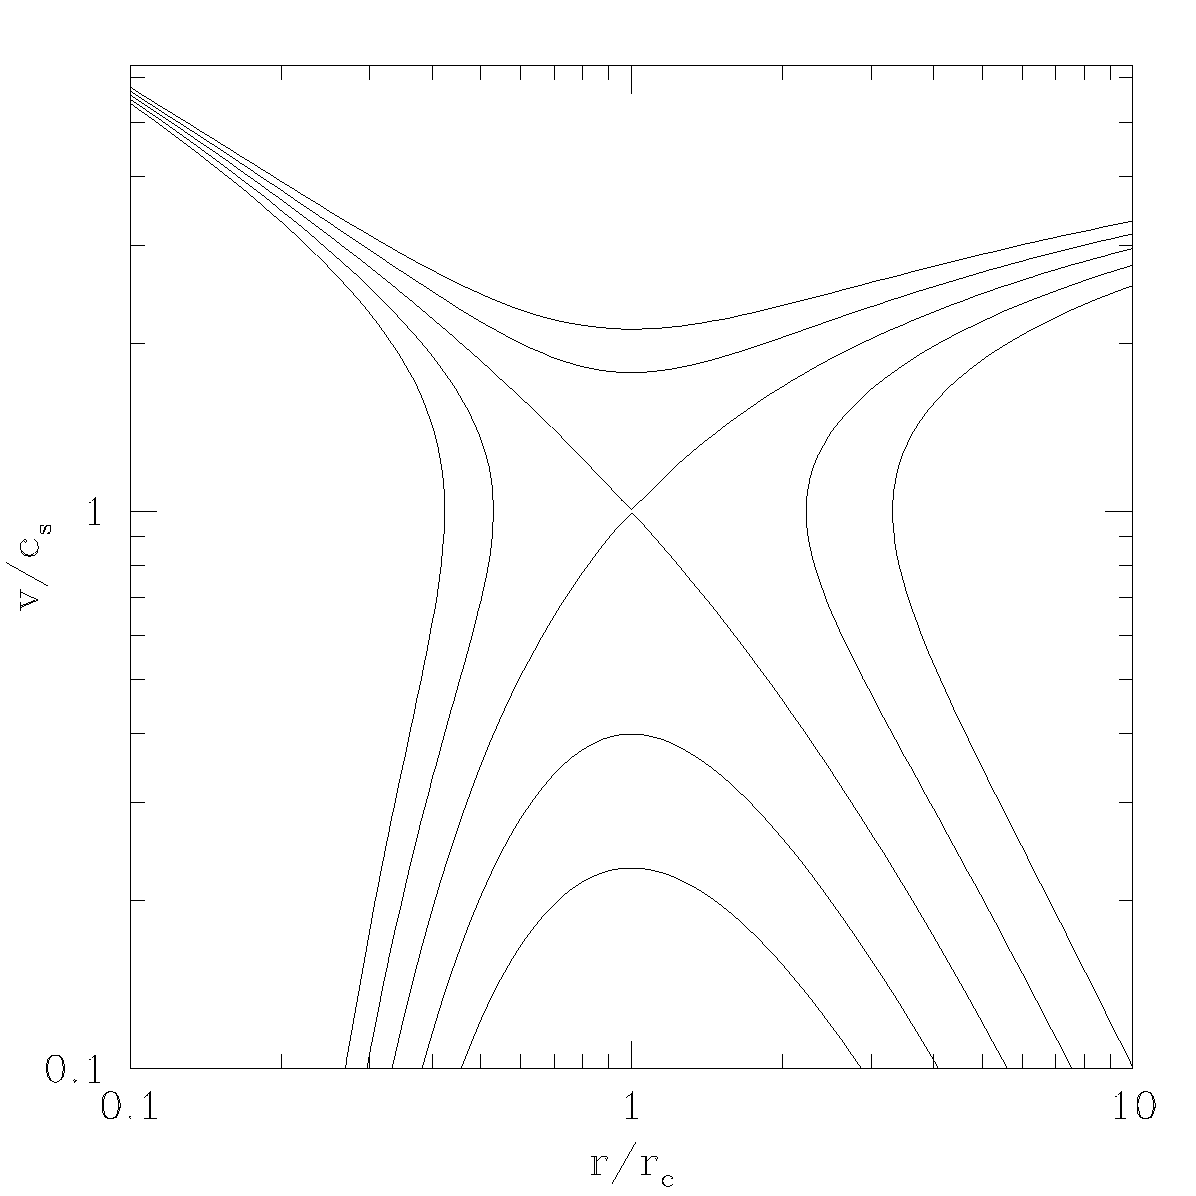
\includegraphics[width=\textwidth]{isothermal} 
\caption{The velocity structure for an isothermal wind, neglecting
  angular momentum and magnetic fields.}
\label{fig:isothermal}
\end{figure}
}

\section{Problems}
\begin{enumerate}


\item{\bf Exact Solutions}

For which values of $\gamma$ can the Bernoulli equation
(Eq.~\ref{eq:725}) be solved using elementary methods (linear,
quadratic and cubic equations of the form in Eq.~\ref{eq:676}).  There
are many, however only a few have $1< \gamma < 5/3$.

\item{\bf Monoatomic Gas}

For a monoatomic gas, the value of $\gamma$ is $5/3$.  According
Eq.~\ref{eq:729}, the density at the critical radius is infinite, and
the critical radius itself goes to zero.  Explain how accretion from
atomic gas would proceed.

\item{\bf Accretion Disk}

  Calculate the surface temperature of the accretion disk as a
  function of radius, central mass and accretion rate.  You may assume
  that all of the energy generated by viscous stresses is radiated
  locally as blackbody emission.  Calculate the cumulative amount of
  flux as a function of temperature.  Does most of the radiation
  emerge from regions at high temperature, at low temperatures or
  somewhere in between?

\item{\bf Bondi Solution}

Generate a picture like Fig.~\ref{fig:bondi} for the Bondi
solution to spherical accretion.  Use $\gamma=9/7$.

\item{\bf Bondi Solution --- Harder}

Generate a Fig.~\ref{fig:bondi} for the Bondi
solution to spherical accretion.  Use $\gamma=7/5$.

\item{\bf Accretion Energetics}

\begin{enumerate}
\item Let's use Newtonian gravity for simplicity here. How much
  kinetic energy does a gram of material have if it falls freely from
  infinity to the surface of a star of mass $M$ and radius $R$?
\item How much energy is released if a gram of material falls from a
  circular orbit just above the stellar surface onto the stellar
  surface? To put it another way, what is the kinetic energy of the
  material in the circular orbit?
\item Hydrogen burning releases about $6 \times 10^{18}$~erg/g. How does
  accretion of hydrogen onto a neutron star ($R=10$~km, $M=1.4 \mathrm{M}_\odot$) differ
  from accretion onto a white dwarf ($R=10000$~km, $M=0.6 \mathrm{M}_\odot$)?
\item What is the total about of energy released per gram of material
  as it falls from infinity to the surface of a neutron star? How many
  grams of material would have to fall each second on the neutron star
  to generate an Eddington luminosity through accretion? This is
  called the Eddington accretion rate.
\end{enumerate}

\item{ \bf A Simplified Accretion Disk }
This is a simplified model for an accretion disk. It is simpler than
the model outlined in the chapter but it will give the
right order of magnitude for things. We are also using Newtonian
gravity.
\begin{enumerate}
\item Let's divide the accretion disk into a series of rings each of
  mass $dm$. What is the total energy of a ring at a distance r from
  the central black hole of mass $M$?

\item Let's say that the ring shrinks by a distance $dr$. What is the
  change in the energy of the ring ($dE/dr$)?  As the ring shrinks mass
  is moving toward the black hole. Divide both sides the answer to (b)
  by $dt$ to get an equation for the energy loss rate per radial
  interval.

\item What is the energy loss rate per unit area?

\item Let's assume that this energy is radiated at the radius where it
  is liberated. Using the blackbody formula what is the temperature of
  the surface of the disk?

\item Let's assume that the disk extends from an outer radius $r_A$ to
  an inner radius $r_0$. What is the total luminosity of the disk if
  the accretion rate is $dm/dt$? What and where is the peak
  temperature of the disk? What and where is the minimum temperature
  of the disk?

\item Sketch the spectrum from the accretion disk on a log-log
  plot. You can use temperature units for the energy axis (i.e. $kT_\mathrm{max}$
  and $kT_\mathrm{min}$). To do this you will have to think about the peak flux
  from a blackbody at a particular temperature and the size of the
  disk that radiates at $T_\mathrm{max}$ and $T_\mathrm{min}$.

\item The accretion rate is determined by the evolution of the orbit
  of the black hole with its companion, so it doesn't know about the
  Eddington limit of the black hole. What do you suppose happens if
  the rate that matter falls onto the disk exceeds the Eddington
  limit?

\item What major bit of physics has been left out of this analysis?
\end{enumerate}
\end{enumerate}
%%% Local Variables:
%%% TeX-master: "book"
%%% End:

\chapter{Fluid Instabities}
\label{cha:fluid-instabities}
\label{sec:instabilities}
\index{fluid mechanics!instabilities}
\section{Gravity Waves and Rayleigh-Taylor Instability}
\label{sec:gravitywaves}
\index{fluid mechanics!gravity waves}
\index{gravity waves}
\index{Rayleigh-Taylor instability}
\index{fluid mechanics!instabilities!Rayleigh-Taylor}

\begin{figure}
\begin{center}
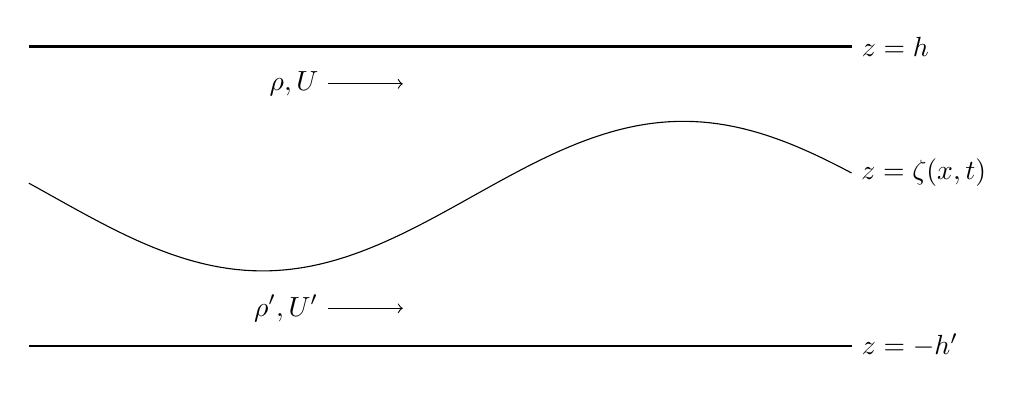
\begin{tikzpicture}[scale=0.95]
\draw [thick] (0,2) -- (11,2) node [right] {$z=h$} (0,-2) -- (11, -2)
node [right] {$z=-h'$} ;
\draw plot [domain=0:11,samples=100] ( \x, {sin(32*\x+170)}) node [right] {$z=\zeta(x,t)$} ;
\draw [<-] (5,1.5) -- (4,1.5) node [left] {$\rho, U$} ; 
\draw [<-] (5,-1.5) -- (4,-1.5) node [left] {$\rho', U'$} ; 
\end{tikzpicture}
\end{center}
\caption{Shearing flow in a stratified fluid}
\end{figure}
Let's imagine a different type of wave on a fluid.  Let's imagine we
have two fluids in a gravitational field.  The lower fluid has density
$\rho'$, velocity $U'$ and thickness $h'$ and the upper fluid has
density $\rho$, velocity $U$ and
thickness $h$.  Let's have $\zeta(x,t)$ denote the displacement of the
interface in the $z-$direction.  Let's assume that both fluids are
incompressible and the flow is irrotational, so we can define
\begin{equation}
{\bf v} = -\nabla \Phi ~\mathrm{and}~ {\bf v}' = -\nabla \Phi'
\end{equation}
where
\begin{equation}
\Phi = -U x + \phi~\mathrm{and}~ \Phi' = -U' x + \phi'.
\end{equation}
To make further progress let us assume that the displacement of the
interface has the form
\begin{equation}
\zeta(x,t) = A \cos \left ( k x - \omega t \right )
\end{equation}
and furthermore let velocity potentials also have a similar dependence
\begin{equation}
  \phi = C \sin \left (k x - \omega t\right ) f(z)~\mathrm{and}~
  \phi' = C' \sin \left (k x - \omega t\right ) f'(z).
\end{equation}
Because the fluids are assumed to be incompressible, we have $\nabla^2
\phi=0$ and the boundary condition gives $\partial \phi/\partial z=0$
at $z=h$ and similarly for lower fluid, so we have 
\begin{eqnarray}
\phi &=& C \sin \left (k x - \omega t\right ) \cosh \left [ k(z-h)
\right ] \\
\phi' &=& C' \sin \left (k x - \omega t\right ) \cosh \left [ k(z+h')
\right ]. 
\end{eqnarray}
The Lagrangian derivative of the displacement of the interface
$D \zeta(x,t)/Dt$ gives the vertical velocity of the fluid at the
interface, so
\begin{equation}
-\pp{\phi}{z} = \pp{\zeta}{t} + U \pp{\zeta}{x}~\mathrm{and}~
-\pp{\phi'}{z} = \pp{\zeta}{t} + U' \pp{\zeta}{x}.
\end{equation}
This yields a relationship between the constants $A$, $C$ and $C'$,
the wavenumber and frequency,
\begin{eqnarray}
A \left ( k U - \omega \right ) &=& - k C \sinh k h, 
\label{eq:868}
\\
A \left ( k U' - \omega \right ) &=&  k C' \sinh k h'.
\label{eq:869}
\end{eqnarray}
We seek a relationship between $\omega$ and $k$, so we require an
additional equation to eliminate the unknowns $A$, $C$ and $C'$.
Specifically, the pressure on each side of the interface must be
equal.  To examine the pressure let's look at Euler's equation
for the ideal fluid (Eq.~\ref{eq:631}) and substitute ${\bf V}=-\nabla
\Phi$ to yield
\begin{equation}
-\pp{\nabla \Phi}{t} + \frac{1}{2} \nabla V^2 = -\frac{\nabla P}{\rho}
- g {\hat z}.
\end{equation}
Since the fluid is incompressible we can write
\begin{equation}
\nabla \left [ -\pp{\Phi}{t} + \frac{V^2}{2} + \frac{P}{\rho} + g h
\right ] = 0,
\end{equation}
so for each fluid we have
\begin{eqnarray}
-\rho \pp{\Phi}{t} + \rho \frac{v^2}{2} + g z \rho + p &=& B(t), \\
-\rho \pp{\Phi'}{t} + \rho' \frac{v'^2}{2} + g \rho' z + p &=& B'(t).
\end{eqnarray}
At the upper and lower surface the velocity of the perturbation
vanishes and $p(z=-h')-p(z=h)$ must equal $g \rho h + g \rho' h'$, so
\begin{equation}
B(t) - B'(t) = \frac{\rho U^2}{2} - \frac{\rho' U'^2}{2}.
\end{equation} 
Let's take the difference of the two Bernoulli equations and evaluate
it at $z=\zeta(x,t)$ to yield
\begin{equation}
\rho \left ( -\pp{\phi}{t} - U \pp{\phi}{x} + g \zeta \right )=
\rho' \left ( -\pp{\phi'}{t} - U' \pp{\phi'}{x} + g \zeta \right ).
\end{equation}
to first order in the small quantities $\phi$ and $\phi'$.
Substituting the expressions for $\phi$, $\phi'$ and $\zeta$ yields
\begin{equation}
\rho \left [ C \cosh kh \left ( \omega - k U \right ) + g A \right ] = 
\rho' \left [ C' \cosh kh' \left ( \omega - k U' \right ) + g A \right ] .
\end{equation}
Combining this result with Eq.~\ref{eq:868} and~\ref{eq:869} yields
the equation,
\begin{equation}
\rho \left ( \omega - k U \right )^2 \coth kh  +
\rho' \left ( \omega - k U' \right )^2 \coth kh' = k g \left (\rho' -
  \rho \right ),
\end{equation}
and the dispersion relation,
\begin{eqnarray}
\frac{\omega}{k} &=& \frac{\rho U \coth kh + \rho' U'\coth k h'}{\rho
  \coth kh + \rho' \coth k h'} \pm \nonumber \\
& &~~~ \left [ \frac{g}{k} \frac{\rho' - \rho}{\rho
  \coth kh + \rho' \coth k h'} - \frac{\rho \rho' \coth kh \coth kh' \left ( U - U' \right )^2}{\left (\rho
  \coth kh + \rho' \coth k h' \right)^2 } \right ]^{1/2}.
\label{eq:870}
\end{eqnarray}
The first interesting limit is where $U=U'=0$ which yields the simpler expression
\begin{equation}
\frac{\omega^2}{k^2} =  \frac{g}{k} \frac{\rho' - \rho}{\rho \coth k h +
    \rho' \coth k h'} 
\label{eq:769}
\end{equation}
If $\rho' > \rho$, then $\omega^2>0$ and we have a stable wave.  There
are several interesting limits to this result.
\begin{itemize}
\item If $\rho=0$, then $\omega^2 = g k \tanh kh$.
\item If $\rho=0$ and $kh \gg 1$, then $\omega^2 = g k$ (deep-water waves).
\item If $\rho=0$ and $kh \ll 1$, then $\omega^2 = g h k^2$ (shallow-water
  waves).
\item If $\rho\neq 0$, $kh' \gg 1$ and $kh \gg 1$, then (both liquids
  very deep)
\begin{equation}
\omega^2 = \frac{kg (\rho' - \rho)}{\rho+\rho'}
\label{eq:770}
\end{equation}
\item If $\rho\neq 0$, $kh' \ll 1$ and $kh \ll 1$, then (long waves)
\begin{equation}
\omega^2 = k^2 \frac{g (\rho' - \rho) h h'}{\rho h'+\rho' h}
\label{eq:771}
\end{equation}
\end{itemize}

On the other hand if $\rho' < \rho$, then $\omega^2 < 0$ and the
perturbation simply grows (it does not oscillate).  This is the
Rayleigh-Taylor instability.  This instability occurs whenever a low
density gas underlies a higher density gas, for example in a supernova
explosion.  The gravitational acceleration $g$ can be due to gravity
(as in a supernova) or due to a deceleration of the fluid, if a
low-density fluid plows into a high-density fluid.  According to
Eq.~\ref{eq:771} the smallest scales have the highest growth rates.
This is countered by viscosity and surface tension, so a
particular scale dominates the growth at least initially.

\section{Kelvin-Helmholtz or Shearing Instability}
\label{sec:kelvin-helmholtz-or}
\index{Kelvin-Helmholtz instability}
\index{shearing instability}
\index{fluid mechanics!instabilities!shearing}

If we look at the term in the brackets in Eq.~\ref{eq:870} for $U \neq
U'$ we see that if $g=0$ waves with all values of $k$ are unstable and if $g\neq
0$ for sufficiently large values of $k$ (small wavelengths), waves are
unstable even if $\rho'>\rho$.  The critical value of $k$ is
\begin{equation}
k_\mathrm{crit} = \frac{g}{\left (U - U'\right)^2} \frac{\rho'-\rho}{\rho \rho' } \frac{\rho
  \coth kh + \rho' \coth k h'}{\coth kh \coth k h'}
\end{equation}
and for $k>k_\mathrm{crit}$ the growth rate increases monotonically.
In reality for really small wavelengths other effects come into play,
such as surface tension and viscosity; therefore, unless the velocity
difference is sufficiently large, waves will not grow, and furthermore
a particular wavelength grow the fastest.

We have also assumed that the velocity change is abrupt.  It turns out
that even if the velocity changes gradually with position, the flow is
unstable, so we would like to get a heuristic understanding of the
Kelvin-Helmholtz instability.  We have two fluids moving in opposite
directions along their shared interface which may be thick.  We do not
include gravity.

Let's assume that the flow is initially steady and
irrotational that so we have Euler's equation
\begin{equation}
({\bf V} \cdot \nabla) {\bf V} + \frac{\nabla P}{\rho} = 0
\label{eq:772}
\end{equation}
We know that 
\begin{equation}
\frac{1}{2} \nabla v^2 = {\bf V} \times (\nabla \times {\bf v}) + ({\bf
  v} \cdot \nabla ) {\bf v}
\label{eq:773}
\end{equation}
which yields
\begin{equation}
\frac{1}{2} \nabla V^2 + \frac{\nabla P}{\rho} = 0
\label{eq:774}
\end{equation}
and
\begin{equation}
\frac{1}{2} V^2 + \frac{P}{\rho} = \rmmat{constant}
\label{eq:775}
\end{equation}
for the flow.  Therefore, regions where $V^2$ is large have lower
pressure.  In the figure we have chosen a reference frame where the fluids
are moving with equal and opposite velocities.   We will also assume
that the depths of both fluids are really large and the densities are
equal.  Therefore, the picture of what goes on in one fluid is
mirrored in the other.    If we focus on the wrinkle in the interface
on the right hand side, the upper fluid must travel a bit farther to
get around the wrinkle than the lower fluid, so it must travel faster
and according to Eq.~\ref{eq:775}, its pressure must drop more than
the fluid below the interface.   The pressure on the inside of the
curve is greater than on the outside.  These pressure gradient causes
the wrinkle to grow.    We could even imagine a rubber sheet or less
dramatically a layer of fluid moving at intermediate velocities lying
along the interface and the forces would still be the same, and the
instability remains.

\begin{figure}
\begin{center}
% \includegraphics[width=\columnwidth]{shear} 
\begin{tikzpicture}
\draw [dashed] (0,0) -- (12,0) ;
\draw plot [domain=0:12,samples=100] ( \x, {sin(32*\x+170)}) ;
\draw [solid] (3.125,-0.85) circle (0.075) (3.125, -1.15) circle (0.075) 
(8.75,0.85) circle (0.075) (8.75, 1.15) circle (0.075) ;
\draw [->] (3.325,-1.4) -- (3.325,-0.6) ;
\draw (3.725,-1.3) node {${\bf \nabla} P$} ;
\draw [->] (8.55,1.4) -- (8.55,0.6) ;
\draw (8.15,1.3) node {${\bf \nabla} P$} ;
\draw [->] (5.5,2) -- (6.5,2) ;
\draw (7,2) node {${\bf v}/2$} ;
\draw [<-] (5.5,-2) -- (6.5,-2) ;
\draw (5,-2) node {$-{\bf v}/2$} ;
\end{tikzpicture}
\end{center}
\caption{Illustration of shearing flow with pressure gradients}
\end{figure}

\section{Gravitational Instability}
\label{sec:grav-inst}
\index{fluid mechanics!instabilities!gravitational}
\index{gravitational instability}

Let's revisit our small sound waves but this time we will include the 
effects of self-gravity.
have 
\begin{equation}
\pp{\rho}{t} + \nabla \cdot (\rho {\bf V}) = \pp{\rho'}{t} + \rho_0
\nabla \cdot {\bf V}' = 0 
\label{eq:776}
\end{equation}
and 
\begin{equation}
\pp{{\bf V}}{t} + \left ( {\bf V} \cdot \nabla \right ) {\bf V} +
\frac{\nabla P}{\rho} =
\dd{\bf V}{t} + \frac{\nabla P}{\rho} =
\pp{{\bf V}'}{t} + \frac{\nabla P'}{\rho_0} = -\nabla \phi'
\label{eq:777}
\end{equation}
We can write $P' = (\partial P/\partial \rho)_s \rho'$ and rewrite the
continuity equation to get
\begin{equation}
\pp{P'}{t} + \rho_0 \left ( \pp{P}{\rho} \right )_s \nabla \cdot {\bf
  V'} = 0
\label{eq:778}
\end{equation}
Let's take the divergence of the Euler equation to get
\begin{equation}
\pp{{\bf \nabla \cdot V}'}{t} + \frac{\nabla^2 P'}{\rho_0} = -\nabla^2 \phi'
\label{eq:779}
\end{equation}
and the time derivative of the continuity equation to get
\begin{equation}
\pp{^2 P'}{t^2} + \rho_0 \left ( \pp{P}{\rho} \right )_s \nabla \cdot \pp{\bf
  V'}{t} = 0.
\label{eq:780}
\end{equation}
Finally we put the two together to get
\begin{equation}
\pp{^2 P'}{t^2} - \left ( \pp{P}{\rho} \right )_s \left ( \nabla^2 P'
+ \rho_0 \nabla^2 \phi' \right ) = 0.
\label{eq:781}
\end{equation}
This is a wave equation with a sound speed of $c_s^2 = (\partial
P/\partial \rho)_s$ but there is an extra term.
\begin{equation}
\nabla^2 \phi' = 4\pi G \rho'
\label{eq:782}
\end{equation}
We can write $P' = c_s^2 \rho'$.  This eliminates density from the
equation to get
\begin{equation}
\pp{^2 P'}{t^2} - c_s^2 \nabla^2 P' - 4\pi G \rho_0 P' = 0.
\label{eq:783}
\end{equation}
Let's try a trial plane wave to find a solution to this equation
\begin{equation}
P' = p' \exp[i({\bf k} \cdot {\bf r} - \omega t)]
\label{eq:784}
\end{equation}
We get
\begin{equation}
-\omega^2 + c_s^2 k^2 - 4\pi G \rho_0 = 0
\label{eq:785}
\end{equation}
so
\begin{equation}
\omega^2 = c_s^2 k^2 - 4\pi G \rho_0.
\label{eq:786}
\end{equation}
If $k^2 > 4\pi G \rho_0/c_s^2$, then $\omega^2>0$ and the wave is
stable.  On the other hand, if $k^2 < 4\pi G \rho_0/c_s^2$, the
perturbation will grow.  We can define a Jeans length
\begin{equation}
l_\rmscr{Jeans} = \frac{2\pi}{k_\rmscr{crit}} =
\sqrt{\frac{\pi}{G\rho_0}} c_s
\label{eq:787}
\end{equation}
and a Jeans mass
\begin{eqnarray}
M_\rmscr{Jeans} &=& \frac{4}{3} \pi l_\rmscr{Jeans}^3 \rho_0 = 
\frac{4}{3} \sqrt{\frac{\pi^5}{G^3 \rho_0}} c_s^3 \\
&=& 1.4 \times 10^{42}\rmmat{g}
  \left [ \frac{\rho_0}{10^{-24} \rmmat{g cm}^{-3}} \right ]^{-1/2} \left [
  \frac{c_s}{10 \rmmat{km s}^{-1}} \right ]^3
\label{eq:788}
\end{eqnarray}

\section{Thermal Instability}
\index{fluid mechanics!instabilities!thermal}
\index{thermal instability}

So far we have examined instabilities where energy does not leave or
enter the fluid.  In general hot gas emits and absorbs radiation; it
may release energy through nuclear or chamical reactions as well.   If
the power absorbed and generated within the gas equals the power
emitted by the gas, the temperature of the gas will remain constant
and equilibrium is achieved.  The question remains whether this
equilibrium is stable.  Heuristically we can see that if the cooling
rate increases faster with temperature than the heating rate, then a
slight increase in temperature will result in the gas cooling faster
and the temperture returning to its equilibruum value.  On the other
hand, if the heating rate increases with temperature faster than the
cooling rate, the slight temperature increase will be compounded with
a further increase in temperature.


\section{Problems}
\begin{enumerate}
\item{\bf X-ray Bursts:}

We will try to model Type-I X-ray bursts using a simple model for the instability. We will calculate how much material will accumulate on a neutron star before it bursts.
\begin{enumerate}
\item Let us assume that the star accretes pure helium, that the
  temperature of the degenerate layer is constant down to the core
  ($T_c$), how much luminosity emerges from the surface of the star? 

\item Let us assume that the helium layer has a mass, $dM$, and that the enregy generation rate for helium burning is given by
$$
\epsilon_{3\alpha} = 3.5 \times 10^{20} T_9^{-3} \exp(-4.32/T_9) \mathrm{erg s}^{-1} \mathrm{g}^{-1}
$$
where $T_9=T/10^9 \mathrm{K}$. The energy generation rate is a
function of density too, but let's forget about that to keep things
simple. How much power does the helium layer generate as a function of
$dM$?

\item Equate your answer to (a) to the answer to (b) and solve for
  $dM$. This is the thickness of a layer in thermal equilibrium.

\item Let's assume that the potential burst starts by the temperature
  in the accreted layer jiggling up by a wee bit. If the surface
  luminosity increases faster with temperature than the helium burning
  rate, then the layer is stable. Calculate $dL_\mathrm{surface}/dT$ and
  $dP_\mathrm{helium}/dT$.

\item Calculate the value of $dM$ for which $dP_\mathrm{helium}/dT$
  exceeds $dL_\mathrm{surface}/dT$ and the layer bursts.

\item Equate your value of $dM$ in (c) and (e) and solve for $T$. What
  is $dM$? How long will it take for such a layer to accumulate if the
  star is accreting at one-tenth of the Eddington accretion rate?

\end{enumerate}
\end{enumerate}
%%% Local Variables:
%%% TeX-master: "book"
%%% End:
%\chapter{Cosmic Rays}

Up to this point the book has focussed either on the propagation and
production of light that we ultimately detect, or the properties of
matter and its motion that produce the light.  The reader might get
the mistaken impression that light is the only messenger from the
matter in the cosmos.   In fact the matter itself is often a messenger
in the form of meteorites, interplanetary and interstellar dust.
However, here the focus will be on the elementary particles and nuclei
that travel to Earth at nearly the speed of light.

\section{Cosmic Ray Production}

\section{Cosmic Ray Propagation}


%%% Local Variables:
%%% TeX-master: "book"
%%% End:

\appendix

\chapter{Mathematical Appendix}
\label{cha:math-append}

\section{The Integral of $x^3/(e^x-1)$}
\label{sec:integral-b_nut}

The integral can be evaluated using a Taylor series
\begin{equation}
\int_0^\infty \frac{x^3}{e^x - 1} d x
= \int_0^\infty \frac{x^3 e^{-x}}{1-e^{-x}} d x =
\int_0^\infty x^3 \sum_{n=1}^{\infty} e^{-nx} d x
\label{eq:796}
\end{equation} 
Let's look at each term in the sum (we can do this because each
term in the sum is a convergent integral)
\begin{equation}
\int_0^\infty x^3 e^{-nx} dx = \frac{1}{n^4} \int_0^\infty u^3 e^{-u}
du.
\label{eq:801}
\end{equation}
The integral 
\begin{equation}
\int_0^\infty u^3 e^{-u} du = \left . -u^3 e^{-u} \right |_0^\infty 
+ 3 \int_0^\infty u^2 e^{-u} du
\end{equation}
and
\begin{equation}
\int_0^\infty u^3 e^{-u} du = 3 \left ( \left . -u^2 e^{-u}
  \right|_0^\infty  + 2 \int_0^\infty u e^{-u} du  \right )
\end{equation}
and
\begin{equation}
\int_0^\infty u^3 e^{-u} du = 3 \times 2 \times \left ( \left . -u e^{-u}
  \right|_0^\infty  + \int_0^\infty e^{-u} du  \right ) = 6
\end{equation}
to yield
\begin{equation}
\int_0^\infty \frac{x^3}{e^x - 1} d x = \sum_{n=1}^\infty \frac{6}{n^4}.
\label{eq:800}
\end{equation}
This result can be generalized to yield
\begin{equation}
\int_0^\infty \frac{x^\alpha}{e^x - 1} d x = \sum_{n=1}^\infty
\frac{\Gamma(\alpha+1)}{n^\alpha} = \Gamma(\alpha+1) \zeta(\alpha+1).
\label{eq:828}
\end{equation}
For odd positive values of $\alpha$ the summation can be solved with contour
integration.  Let's start with
$$
\sum_{n=1}^\infty \frac{1}{n^4}
$$ 
to evaluate.  We will use a basic result from complex analysis that
the integral of an analytic function around a closed contour vanishes
if the contour contains no poles.  Let's examine the function
\begin{equation}
f(z) = \frac{\pi \cot (\pi z)}{z^4} dz
\label{eq:795}
\end{equation}
that has poles at $z= \ldots, -2, -1, 0, 1, 2 \ldots$ and for large
values of $z$ $f(z)$ quickly approaches zero, so the integral 
\begin{figure}
\begin{center}
\begin{tikzpicture}
\foreach \x in {1,...,4} {
\fill (\x,0) circle (0.05) ;
\fill (-\x,0) circle (0.05) ;
}
\draw (0,0) circle (0.05);
\foreach \x in {-4,...,4} {
\draw [->] (\x,0.2) arc (90:360:0.2) arc (0:90:0.2);
}
\draw [->] (-5,0) -- (5,0);
\draw [->] (0,-2) -- (0,2);
\end{tikzpicture}
\end{center}
\caption{The poles of $f(z)$ in the complex plane}
\label{fig:polesfz}
\end{figure}
\begin{equation}
\lim_{R\rightarrow \infty }\oint_{C_R} f(z) dz = 0
\label{eq:797}
\end{equation}
where $C_R$ is a circle of radius $R$.  The sum of the integrals about
all of the poles must vanish.  Fig.~\ref{fig:polesfz} shows all of the
poles.  At the poles (solid points in the figure) other than at the
origin, the function is given by
\begin{equation}
f(z) \approx \frac{1}{n^4} \frac{1}{z-n}
\label{eq:798}
\end{equation}
that we can integrate along the loops in the figure by substituting
$z=n+R e^{i\theta}$ so $dz = i R e^{i\theta} d\theta$ and
\begin{equation}
\lim_{R\rightarrow 0} \oint_{C_R} f(z) dz = 
\lim_{R\rightarrow 0} \int_0^{2\pi} \frac{1}{n^4} \frac{1}{R e^{i\theta}} i R
e^{i\theta} d\theta = \frac{i}{n^4} \int_0^{2\pi} d\theta = 2\pi i \frac{1}{n^4}
\label{eq:829}
\end{equation}
where $C_R$ is a circle of radius $R$ centered on the pole.   Let's
combine this result with the integral around the large loop
(Eq.~\ref{eq:797}) to give
\begin{equation}
0 = 4\pi i \sum_{n=1}^\infty \frac{1}{n^4} + \lim_{R\rightarrow 0}
\oint_{C_R} f(z) dz
\label{eq:799}
\end{equation}
where the first term is the sum we seek and the second term is an
integral is over a circle surrounding the origin.  The leading term in
the integral about the origin is proportional to $z^{-5}$ and $\oint
z^{-n} dz=0$ if $n\neq 1$, so we have to look at higher order terms,
specifically
\begin{equation}
f(z) = \frac{1}{z^5} - \frac{\pi^2}{3 z^3} - \frac{\pi^4}{45 z} +
\cdots 
\label{eq:803}
\end{equation}
so we have
\begin{equation}
0 = 4\pi i \sum_{n=1}^\infty \frac{1}{n^4} + 2\pi i \left ( -
  \frac{\pi^4}{45} \right )
\label{eq:802}
\end{equation}
and 
\begin{equation}
 \sum_{n=1}^\infty \frac{6}{n^4} = 6 \frac{\pi^4}{45\times 2} = \frac{\pi^4}{15}.
\end{equation}

\section{Parseval's Theorem}
\label{sec:an-math-asid}
\index{Fourier transform!Parseval's theorem}

We have stated a rather useful result,
\begin{equation}
\int_{-\infty}^{\infty} |E(t)|^2 dt = 2\pi \int_{-\infty}^{\infty} 
|{\hat E}(\omega)|^2 d \omega.
\label{eq:159}
\end{equation}
We now have the tools to prove it quickly,
\begin{eqnarray}
\int_{-\infty}^{\infty} |E(t)|^2 dt &=& \int_{-\infty}^{\infty} d t
  \int_{-\infty}^{\infty} {\hat E}(\omega')
e^{-i\omega' t} d \omega'.
  \int_{-\infty}^{\infty} {\hat E}^*(\omega)
e^{i\omega t} d \omega \\
&=& \int_{-\infty}^{\infty}  \int_{-\infty}^{\infty}
  \int_{-\infty}^{\infty} d t d\omega' d \omega
 {\hat E}(\omega') {\hat E}^*(\omega)
e^{-i\omega' t} e^{i\omega t} 
\label{eq:160}
\end{eqnarray}
The integral over time is simply Fourier transform of $2\pi
e^{-i\omega' t}$ which we know,
\begin{eqnarray}
\int_{-\infty}^{\infty} |E(t)|^2 dt &=& 2\pi 
\int_{-\infty}^{\infty}
  \int_{-\infty}^{\infty} d\omega' d \omega
 {\hat E}(\omega') {\hat E}^*(\omega) \delta (\omega -\omega') \\
 &=& 2 \pi \int_{-\infty}^{\infty} d \omega
 {\hat E}(\omega) {\hat E}^*(\omega) =2 \pi \int_{-\infty}^{\infty}
 |{\hat E}(\omega)|^2  d \omega
\label{eq:161}
\end{eqnarray}


%%% Local Variables:
%%% TeX-master: "book"
%%% End:
\chapter{Selected Solutions}

\ifx\bookloaded\undefined
\documentclass{article}
\usepackage{graphicx}
\newcommand{\be}{\begin{equation}}
\newcommand{\ee}{\end{equation}}
\newcommand{\rmmat}[1]{\hbox{\rm #1}}
\newcommand{\rmscr}[1]{{\hbox{\rm \scriptsize #1}}}
\newcommand{\comment}[1]{\relax}
\begin{document}
\fi
\section{Chapter 1}

\begin{enumerate}
\item{\bf Hot Cloud}

X-ray photons are produced in a cloud of radius $R$ at the uniform rate
 (photons per unit volume per unit times). the cloud is a distance $d$
away. Assume that the cloud is optically thin. A detector at Earth has
an angular acceptance beam of half-angle $\Delta \theta$ and an effective area $A$.
\begin{enumerate}
\item If the cloud is fully resolved by the detector, what is the observed 
      intensity of the radiation as a function of position?
\item If the cloud is fully unresolved, what is the average intensity when 
      the source is in the detector?
\end{enumerate}
{\bf Answer:}    
\begin{enumerate}
\item If the source is resolved, we can discern different parts of the cloud, so the observed intensity is the integral of the emission coefficient through the cloud,
\begin{equation}
I = \int j ds = \int_{-\sqrt{R^2-b^2}}^{\sqrt{R^2-b^2}} \frac{\Gamma}{4\pi}  ds = \frac{\Gamma}{2\pi} \sqrt{R^2-b^2} = \frac{\Gamma}{2\pi} R \sqrt{1-\frac{b^2}{R^2}}
\end{equation}
where $b/R$ is the relative distance between our line of sight and the centre of the cloud.
\item If the source is not resolved, the observed intensity is given by the flux from the source divided by the solid angle of acceptance of the detector.
\begin{equation}
I = \frac{F}{\pi \Delta \theta^2} = \frac{\frac{4}{3} \pi R^3 \Gamma  }{4\pi d^2} \frac{1}{\pi \Delta \theta^2} = \frac{\Gamma R^3}{3 \pi d^2 \Delta \theta^2}
\end{equation}

Clearly, this is the minimum value of the actual intensity of the
source because it may actually subtend a smaller region of the sky
that $\Delta \theta$ but we have no way of know because our detector
cannot resolve below this scale.
\end{enumerate}
\setcounter{enumi}{2}
\item{\bf Blackbody}

Only one or no neutrinos can occupy a single state. Calculate the spectrum of the neutrino field in thermal equilibrium (neglect the mass of the neutrino). Neutrinos like photons have two polarization states. What is the ratio of the Stefan-Boltzmann constant for neutrinos to that of photons? 

{\bf Answer:}

The main difference between the neutrinos and the photons is the partition function.  The mean energy of the neutrinos with a certain value of $\nu$ is
\begin{equation}
{\bar E} = \frac{\sum_{i=0}^1 n h \nu e^{-n h\nu/kT}}{\sum_{i=0}^1 e^{-n h\nu/kT}}.
\end{equation}
For photons the sum is from 0 to infinity.  So we have
\begin{equation}
B_\nu (T) = \frac{2 h}{c^2} \frac{\nu^3}{\exp ( h \nu / k T) + 1}.
\end{equation}
for neutrinos.   The ratio of the Stefan-Boltzmann constants is
\begin{equation}
R = \frac{\int_0^\infty x^3 ( e^x + 1 )^{-1}}{\int_0^\infty x^3 (e^x - 1)^{-1}} = \frac{7 \pi^4/120}{\pi^4/15} = \frac{7}{8}
\end{equation}
\setcounter{enumi}{3}
\item {\bf Surface Emission from the Crab Pulsar:}  The neutron star
  that powers the Crab Pulsar can be assumed to have a mass of
  $1.4\mathrm{M}_\odot$ and a radius of 10~km with constant internal
  density and an effective temperature of $10^6$~K.  The frequency of
  the Crab Pulsar is 30~Hz and its period increases by 38 ns each
  day.  Compare the power from the surface emission to the power
  lost as the neutron star spins down.  The total power of the Crab
  Nebulae is about 75,000 times that of the Sun.  What is the likely
  source of this power?

{\bf Answer:}

The blackbody flux from the surface of the star is given by
\begin{equation}
F = 4 \pi R^2 \sigma T^4 = 7 \times 10^{32}~\mathrm{erg/s} = 7 \times 10^{25}~\mathrm{W} = 0.17 \mathrm{L}_\odot.
\end{equation}

As the neutron star spins down it loses kinetic energy at a rate
\begin{equation}
\frac{dE}{dt} = - I \Omega \dot \Omega = - 4\pi^2 \nu^3 I {\dot P} = 
-5 \times 10^{38}~\mathrm{erg/s} = -5 \times 10^{31}~\mathrm{W} = 10^{5}\mathrm{L}_\odot
\end{equation}
where $I \approx \frac{2}{5} M R^2 \approx 10^{45} \mathrm{g cm}^2$.
The spin-down power is approximately the power needed to power the
nebula so it is a possible source of energy.

\item {\bf Power-Law Atmosphere}

Assume the following
\begin{itemize}
\item The Rosseland mean opacity is related to the density and 
temperature of the gas through a power-law relationship,
      \begin{equation}
      \kappa_R = \kappa_0 \rho^\alpha T^\beta;
      \end{equation}
\item The pressure of the gas is given by the ideal gas law;
 \item The gas is in hydrostatic equilibrium so $p=g\Sigma$  where 
      $g$ is the surface gravity; and
 \item The gas is in radiative equilibrium with the radiation 
      field so the flux is constant with respect to $z$ or $\Sigma$.
    \end{itemize}
Calculate the temperature of the gas as a function of $\Sigma$.

{\bf Answer:}

First we take the equation of radiative transfer

\begin{equation}
F(z) = -\frac{16 \sigma T^3}{3\kappa_R} \frac{\partial T}{\partial \Sigma} = 
\frac{16 \sigma T^3}{3\kappa_0 \rho^\alpha T^\beta} \frac{\partial T}{\partial \Sigma}
\end{equation}
We eliminate the variable $\rho$ using the ideal gas law and the equation of
hydrostatic equilibrium,
\begin{equation}
g_s \Sigma = \frac{1}{\mu m_p} \rho k T
\end{equation}
so we have
\begin{equation}
\frac{\partial T}{\partial \Sigma} = \frac{3\kappa_0 }{16 \sigma F}
\Sigma^\alpha T^{\beta-\alpha-3} \left ( \frac{\mu m_p}{g_s k} \right )^\alpha
\end{equation}
which can be integrated by the separation of variables to yield
\begin{equation}
\frac{T^{4+\alpha-\beta}}{4+\alpha-\beta} = \frac{3\kappa_0 }{16 \sigma F}
\frac{\Sigma^{\alpha+1}}{\alpha+1}  \left ( \frac{\mu m_p}{g_s k} \right )^\alpha
\end{equation}
\setcounter{enumi}{6}
\item{\bf Goggles}

Calculate from thermodynamic principles how much objects are magnified or demagnified while viewed through goggles underwater. N.B. The wavenumber of a photon of a given frequency is proportional to the index of refraction.

{\bf Answer:}

If we have a blackbody underwater and a blackbody in air at equal temperatures, the underwater blackbody will emit
\begin{equation}
F_{water} = n^2 F_{air}
\end{equation}
energy per unit area per unit time.  You can see this from the definition of the density of states
\begin{equation}
\rho_s = 4\pi k^2 d k = 4\pi \left ( \frac{n \nu}{c} \right )^2 d \left (\frac{n \nu}{c} \right )
\end{equation}
which is larger by a factor of $n^3$, so the energy density within the water of the blackbody radiation is larger by a factor of $n^3$ than in air.   However, flux is related to the intensity which is energy density times the velocity so the flux is only larger by a factor of $n^2$.

For the underwater blackbody to absorb as much as radiation from the
blackbody in air as the blackbody in air receives from it, the solid
angle subtended by the underwater BB must be larger by $n^2$
so it is magnified linearly by a factor of$n\approx 1.33$.
\end{enumerate}

\ifx\bookloaded\undefined
\end{document}
\end
\fi

%%% Local Variables:
%%% TeX-master: "book"
%%% End:
\ifx\bookloaded\undefined
\documentclass{article}
\usepackage{graphicx}
\input book_defs
\begin{document}
\fi
\section{Chapter 2}
\begin{enumerate}
\item{\bf  Coulomb's Law}

Derive Coulomb's law from Maxwell's Equations

{\bf Answer:}

The first of Maxwell's equations is
\begin{equation}
\nabla \cdot {\vec E} = 4 \pi \rho
\end{equation}
Let's assume that there is a single charge q located at r=0 and integrate over a spherical region centered on the origin we get
\begin{equation}
\int_V dV \nabla \cdot {\vec E} = \int dV 4 \pi \rho = 4 \pi q
\end{equation}
However the integral of the left-hand side is a integral of a divergence over a volume so we have
\begin{equation}
\int_{\partial V} dV \nabla \cdot {\vec E} = \int {\vec E} \cdot d A = |{\vec E}| 4 \pi R^2 = 4 \pi q
\end{equation}
so 
\begin{equation}
{\vec E} = \frac{q}{R^2} {\hat r}
\end{equation}

\item{\bf Ohm's Law}

In certain cases the process of aborption of radiation can be treated
by means of the macroscopic Maxwell equations. For example, suppose we
have a conducting medium so that the current density j is related to
the electric field E by Ohm's law: 
${\vec j} = \sigma {\vec E}$ where
$\sigma$ is the conductivity (cgs unit = sec$^{-1}$</sup>). 
Investigate the propagation of electromagnetic waves in such a medium
and show that:
\begin{enumerate}
\item
 The wave vector ${\vec k}$ is complex
 ${\vec k}^2 = \frac{\omega^2 m^2}{c^2}$
 where $m$ is the complex index of refraction with
 \begin{equation}
     m^2 = \mu \epsilon \left ( 1 + \frac{4 \pi i \sigma}{\omega \epsilon}
         \right )
         \end{equation}
\item The waves are attenuated as they propagate, corresponding to an
          absorption coefficient.
          \begin{equation}
          \alpha = \frac{2\omega}{c} \Im (m)
          \end{equation}

{\bf Answer:}

Let's take the third and fourth of Maxwell's equations
\begin{equation}
{\nabla} \times {\vec E} = -\frac{1}{c} \frac{\partial \vec B}{\partial t}
\end{equation}
and
\begin{equation}
{\nabla} \times {\vec H} = \frac{4\pi}{c} {\vec J} +\frac{1}{c} 
\frac{\partial \vec D}{\partial t} 
\end{equation}
Let's substitute
\begin{equation}
\mu {\vec H}={\vec B}, {\vec D}=\epsilon {\vec E}
\end{equation}
and
\begin{equation}
{\vec J} = \sigma {\vec E}
\end{equation}
to get
\begin{equation}
{\nabla} \times {\vec B} = \mu \sigma \frac{4\pi}{c} {\vec E} +\frac{1}{c} 
\mu \epsilon \frac{\partial \vec E}{\partial t} 
\end{equation}
Let's take the curl of this equation to get 
\begin{equation}
-{\nabla}^2 {\vec B} = \mu \sigma \frac{4\pi}{c} \nabla \times {\vec E} +\frac{1}{c} 
\mu \epsilon \frac{\partial \nabla \times \vec E}{\partial t} 
\end{equation}
and substitute in the other Maxwell's equation to get
\begin{equation}
-{\nabla}^2 {\vec B} = -\mu \sigma \frac{4\pi}{c^2} \frac{\partial \vec B}{\partial t} - \frac{1}{c^2} 
\mu \epsilon \frac{\partial^2 \vec B}{\partial t^2}
\end{equation}
Let's substitute 
\begin{equation}{\vec B} = {\vec B}_0 \exp \left [ i \left ({\vec k}\cdot {\vec x} - \omega t \right ) \right ]\end{equation} 
to get
\begin{equation}
k^2 = i \mu \sigma \frac{4\pi}{c^2} \omega + \frac{1}{c^2} 
\mu \epsilon \omega^2 = \frac{\omega^2 m^2}{c^2}
\end{equation}
with
\begin{equation}
m^2 = \mu \epsilon \left ( 1 + i \frac{4\pi\sigma}{\omega \epsilon} \right )
\end{equation}
If we substitute this into the formula for the wave we find
\begin{equation}
{\vec B} = {\vec B}_0 \exp \left [ i \left ({\vec k}\cdot {\vec x} - \omega t \right ) \right ]
= {\vec B}_0 \exp \left [ i \left (\Re {\vec k}\cdot {\vec x} - \omega t \right ) \right ]
\exp \left [ -\Im {\vec k} \cdot {\vec x} \right ] 
\end{equation}
so the magnetic field decreases with a mean-free path $\frac{c}{\omega
  \Im m}$.  The energy is proportional to $B^2$ so the absorption coefficient is $\frac{2\omega}{c}\Im
m$
\end{enumerate}
\item {\bf The Edge of the Crab}

  Fig.~\ref{fig:crab-edge} shows the x-ray emission of the Crab pulsar
  wind nebula at a distance of 2~kpc.  The x-ray emitting gas is
  contained by magnetic fields causing the x-ray emission regions to
  end sharply.  We can relate the frequency of the emission to the energy
  of the electrons and the strength of the magnetic field by
\begin{equation}
\omega = \left ( \frac{E}{m_e c^2}
\right )^2 \frac{e B}{m_e c} 
\end{equation}
and assume that the electrons are relativistic so their inertial mass
is $E/c^2$.  Use the sharpness of the emission
regions to determine the energy of the electrons and the strength of
the magnetic field.

{\bf Answer:}

Let's assume that the particles are doing cyclotron motion so
\begin{equation}
F = \frac{m v^2}{r} = \frac{ e v B}{c}, v\approx c, m\approx
\frac{E}{c^2}
\end{equation}
so
$$
\frac{E}{r} = e B, E = e B r
$$
where $r < 2~\mathrm{kpc} \times 1~\mathrm{arcsecond} = 2000~\mathrm{AU}$
and we also know that $\omega$ lies in the X-rays, so $\hbar \omega \sim
1$~keV and
$$
\omega = E^2 B \frac{e}{m_e^3 c^5} = E^2 \frac{E}{er} \frac{e}{m_e^3 c^5}
$$
so
$$
E^3 = m_e^3 c^5 \omega r, B^3 = \frac{m_e^3 c^5 \omega}{e^3 r^2}.
$$
The fact the the edge is unresolved yields an upper limit on the energy
and a lower limit on the magnetic field strength.  If we use $\hbar
\omega=1~\mathrm{keV}$, we obtain
$$
E < 6 \times 10^{13}~\mathrm{eV}, B > 7 \times 10^{-11}~\mathrm{G}
$$


\item{\bf Momenta}
This problem is meant to deduce the momentum and angular momentum
properties of radiation and does not recesarily represent any real
physical system of interest. Consider a charge $Q$ in a viscous medium
where the viscous force is proportional to velocity: 
\begin{equation}
F_{visc} = -\beta v
\end{equation}
Suppose a circular polarized wave passes through the medium. The
equation of motion of the charge is 
\begin{equation}
m \frac{dv}{dt} = F_{visc} + F_{Lorentz}
\end{equation}
We assume that the terms on the right dominate the inertial term on the
left, so that approximately 
\begin{equation}
0 = F_{visc} + F_{Lorentz}
\end{equation}
Let the frequency of the wave be $\omega$ and the strength of the
electric field be E.
\begin{enumerate}
\item Show that to lowest order (neglecting the magnetic force) the charge
   moves on a circle in a plane normal to the direction of propagation of
   the wave with speed $QE/\beta$ and with radius $QE/(\beta \omega)$.
\item Show that the power transmitted to the fliud by the wave is $Q^2 E^2/\beta$
\item. By considering the small magnetic force acting on the particle show
   that the momentum per unit time (force) given to the fluid by the wave
   is in the direction of propagation and has the magnitude 
   $Q^2 E^2/(\beta c)$.
\item Show that the angular momentum per unit time (torque) given to the
   fluid by the wave is in the direction of propagation and has magnitude
   $\pm Q^2 E^2/(\beta \omega)$ where the $+$ is for left and $-$ is for
   right circular polarization.
\item Show that the absorption cross section of the charge is
   $4\pi Q^2/(\beta c)$.
\item  If we regard the radiation to be composed of circular polarized
   photons of energy $E_\gamma= h \nu$, show that these results imply that the
   photon has momemtum $p=h/\lambda=E_\gamma/c$ and has angular momemtum 
   $J=\pm \hbar$ along the direction of propagation.
\item Repeat this problem for a linearly polarized wave
\end{enumerate}

{\bf Answer:}

\begin{enumerate}
\item
 We have ${\vec v} = \frac{Q}{\beta} {\vec E}$.  The electric field traces a circle so the 
particle traces a circle with a speed $\frac{QE}{\beta}$.  The angular velocity of the particle is $\omega$ of the wave, so $\omega r=\frac{QE}{\beta}$ so $r=\frac{QE}/{\beta\omega}$.

\item Power is $Q{\vec v}\cdot {\vec E} = \frac{Q^2 E^2}{\beta}$.

\item The magnetic force is in the direction ${\vec v}\times {\vec B}$ but the velocity points in the
direction of the electric field so the force is in the direction ${\vec E}\times {\vec B}$, the direction of propagation.   The magnitude of magnetic field equals that of the electric field so we have
$F = \frac{Q^2 E^2}{\beta c}$

\item Torque is ${\vec r} \times {\vec F} = \frac{Q^2 E^2}{\beta \omega}$ 

\item The cross section is power absorbed divided by the Poynting vector 
\begin{equation}
\sigma = \frac{Q^2 E^2}{\beta} \left [ \frac{c}{4\pi} E^2 \right ]^{-1} = \frac{4 \pi Q^2}{\beta c}
\end{equation}

\item If the wave comes in energy units of $h\nu$.  The ratio of the momentum unit to the energy unit must 
be the ratio of the force (momentum per unit time) to the power (energy per unit time), so we get
\begin{equation}
h\nu \frac{Q^2 E^2}{\beta c} \frac{\beta}{Q^2 E^2} = \frac{h\nu}{c}
\end{equation}
The ratio of the angular momentum unit to the energy unit must be the
ratio of the torque (angular momentum per unit time) to the power
(energy per unit time), so we get
\begin{equation}
h\nu \frac{Q^2 E^2}{\beta \omega} \frac{\beta}{Q^2 E^2} = \frac{h\nu}{\omega} = \hbar
\end{equation}
\item For the linearly polarized wave, the particle moves up and down sinusoidally.  The size of the up and down path is twice the value of R above (the circle is squished along one axis to be a line).  The velocity varies sinusoidally, the power magnetic force vary as $\sin^2 \omega t$.  The torque vanishes.  The cross section is the same as is the momentum of a photon.  The angular momentum vanishes (because the torque vanishes).
\end{enumerate}


\item{\bf Maxwell before Maxwell}

Show that Maxwell's equations before Maxwell, that is, without the
``displacement current'' term, $c^{-1} \frac{\partial D}{\partial t}$, unacceptably constrained the
sources of the field and also did not permit the existence of waves.

{\bf Answer:}

Let's take the divergence of the Maxwell's equation
\begin{equation}
{\nabla} \times {\vec H} = \frac{4\pi}{c} {\vec J} +\frac{1}{c} 
\frac{\partial \vec D}{\partial t} 
\end{equation}
to get
\begin{equation}
0 = \frac{4\pi}{c} \nabla \cdot {\vec J} 
\end{equation}
where we have left the displacement current out.  This states that the
divergence of the current must vanish, which means that either charge
is not conserved or that the charge density is constant (neither is
good).

Let's take the curl of the Maxwell's equation
\begin{equation}
{\nabla}^2 {\vec B} = 0
\end{equation}
and we would get the same thing for the electric field.  This is not a
wave equation.

\item {\bf Coulomb gauge} 
Derive the equations describing the dynamics of the electric and
vector potentials in the Coulomb gauge
$$
\nabla \cdot {\bf A} = 0
$$
Look at the equation for the electric potential. What is the solution
to the electric potential given the charge density $\rho$? Why is this
called the Coulomb gauge?

How does the expression for the scalar potential in the Coulomb gauge
differ from that in the Lorenz gauge? What is strange about it? Is it
physical?

Now look at the equation for the vector potential. Show that the LHS
can be arranged to be the same as in the Lorenz gauge but the RHS is
not just the current but the current plus something else.

Show that the RHS can be expressed as 
$$
\frac{4\pi}{c} \left ( {\bf J} - {\bf J}_\rmscr{long} \right ) 
$$
where
$$
{\bf J}_\rmscr{long} = -\frac{1}{4\pi} \nabla \int \frac{\nabla' \cdot
{\bf J}}{|{\bf x}-{\bf x}'|} d^3 x
$$

{\bf Answer:}
In the Coulomb gauge the scalar potential follows Coulomb's law
$$
\nabla^2 \phi = -4\pi \rho.
$$
That is why it is called the Coulomb gauge.  The potential everywhere
right now depends on the charge here right now, so it is acausal
(strange); however, because we cannot actually measure the scalar
potential the acausality has no physical consequence.

Now for the vector potential
$$
\nabla^2 {\bf A} - \frac{1}{c^2} \pp{^2 {\bf A}}{t^2} - \nabla \left
  ( \frac{1}{c} \pp{\phi}{t} \right ) = -\frac{4\pi}{c} {\bf J}
$$
$$
\nabla^2 {\bf A} - \frac{1}{c^2} \pp{^2 {\bf A}}{t^2}  =
-\frac{4\pi}{c} \left ( {\bf J} - {\bf J}_\mathrm{long} \right )
$$
where
\begin{eqnarray*}
{\bf J}_\mathrm{long} &=& \frac{1}{4\pi} \nabla \left
  ( \pp{\phi}{t} \right ) =  \frac{1}{4\pi} \nabla \left 
  ( \int \pp{\rho}{t} \frac{1}{\left |{\bf x} - {\bf x}'\right|} d^3 x
\right ) \\
&=& -\frac{1}{4\pi} \nabla \left 
  ( \int \frac{\nabla \cdot {\bf J}}{\left |{\bf x} - {\bf x}'\right|} d^3 x
\right )  = -\frac{1}{4\pi} \nabla \left 
  ( \int \frac{\nabla' \cdot {\bf J}}{\left |{\bf x} - {\bf x}'\right|} d^3 x
\right )  
\end{eqnarray*}
What remains of the current after subtracting the longitudinal current
is the transverse current which is given by the expression
$$
{\bf J}_\mathrm{trans} = \frac{1}{4\pi} \nabla \times \nabla \left 
  ( \int \frac{{\bf J}}{\left |{\bf x} - {\bf x}'\right|} d^3 x
\right )  
$$
so the source for the wave equation for ${\bf A}$ is given by the
transverse current alone.
\end{enumerate}

\ifx\bookloaded\undefined
\end{document}
\fi
%%% Local Variables:
%%% TeX-master: "book"
%%% End:




\ifx\bookloaded\undefined
\documentclass{article}
\usepackage{graphicx}
\usepackage{tikz}
\usetikzlibrary{snakes}
\usetikzlibrary{arrows}
\usetikzlibrary{shapes}
\usetikzlibrary{backgrounds}
\input book_defs
\begin{document}
\fi
\section{Chapter 3}
\begin{enumerate}
\item{\bf Constant Velocity Charge}

Show that if charge is not accelerating, the electric field vector
points to the current (not the retarded) position of the charge.

{\bf Answer:}

\begin{center}
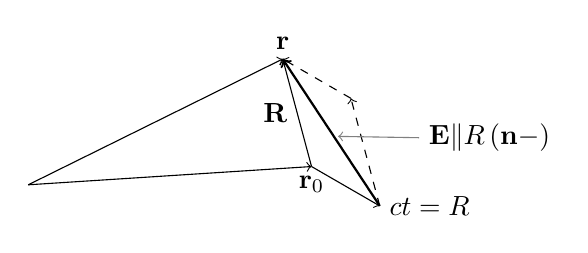
\begin{tikzpicture}
\begin{scope}[rotate=-30]
\draw [->] (0,0)--(2,3);
\draw [->] (0,0)--(3,2);
\draw [->] (3,2)--(4,2) ;
\draw [->] (3,2)--(2,3) ;
\draw [->,dashed] (4,2)--(3,3) ;
\draw [->,dashed] (3,3)--(2,3) ;
\draw [->,thick] (4,2)--(2,3) ; 
\draw (3,2) node [below] {${\bf r}_0$} 
(4,2) node [right] {$\betabold c t=\betabold R$} 
(2,3) node [above] {${\bf r}$} 
(2.5,2.5) node [left] {${\bf R}$}
(4,3) node [right] {${\bf E} \| R\left ({\bf n}-\betabold\right)$};
\draw [->,gray] (4,3)--(3.1,2.5);
\end{scope}
\end{tikzpicture}
\end{center}

\setcounter{enumi}{3}

\item{\bf Synchrotron Cooling:}

A particle of mass $m$, charge $q$, moves in a plane perpendicular to
a uniform, static, magnetic field $B$.
\begin{enumerate}
\item
Calculate the total energy radiated per unit time, expressing it in
terms of the constants already defined and the ratio
$\gamma=1/\sqrt{1-\beta^2}$ of the particle's total energy to its rest 
energy.  You can assume that the particle is ultrarelativistic.
\item
If at time $t=0$ the particle has a total energy $E_0=\gamma_0 m c^2$,
show that it will have energy $E=\gamma m c^2 < E_0$ at a time $t$,
where
\[
t \approx \frac{3 m^3 c^5}{2 q^4 B^2} \left ( \frac{1}{\gamma} -
\frac{1}{\gamma_0} \right ).
\]
\end{enumerate}

{\bf Answer:}

The synchrotron power is given by the power emitted by a particle
performing circular motion
$$
P_\perp = \frac{2}{3} \frac{q^2}{m^2 c^3} \gamma^2 \left ( \frac{d
    {\bf p}}{dt} \right )^2
$$
where for an ultrarelativistic charged particle in a magnetic field we
have
$$
\left | \frac{d {\bf p}}{dt} \right | = q B
$$
so
$$
P_\perp =  \frac{2}{3} \frac{q^5}{m^2 c^3} \gamma^2 B^2 = -\frac{d
  E}{dt} = -m c^2 \frac{d \gamma}{dt}
$$
and
$$
\frac{d \gamma}{dt} = -\frac{2}{3} \frac{q^5}{m^3 c^5} B^2 \gamma^2.
$$
Separating the variables and integrating yields the required answer.

\item{\bf Classical HI:}
A particle of mass $m$ and charge $q$ moves in a circle due to a force 
${\bf F} = -\hat{\bf r} \frac{q^2}{r^2}$.  
You may assume that the particle always moves  non-relativistically.
\begin{enumerate}
\item What is the acceleration of the particle as a function of $r$?
\item What is the total energy of the particle as a function of $r$?
  The potential energy is given by $-q^2/r$.
\item What is the power radiated as a function of $r$?
\item Using the fact the $P=-dE/dt$ and the answer to (2), find
  $dr/dt$. 
\item Assuming that the particle starts with $r=r_i$ at $t=0$, find
  the value of $t$ where $r=0$.   
\item Let's assume that $q=e$, the charge of the electron, and
  $m=m_e$, the mass of the electron.  Write your answer in (4) in
  terms of $r_i$, $r_0$ (the classical electron radius) and $c$.
\item What is the time if $r_i=0.5$\AA (for an hydrogen)?
\item Compare this to the lifetime of a hydrogen atom.
\end{enumerate}

{\bf Answer:}

\begin{enumerate}
\item 
\[ \dot{\bf u} = -{\hat r} \frac{q^2}{r^2 m} \]
\item
\[ E = -\frac{q^2}{r} + \frac{1}{2} m v^2 = -\frac{q^2}{r} + \frac{1}{2} \left ( \frac{q^2}{r} \right ) = -\frac{1}{2} \frac{q^2}{r} \]
where I used
\[ \frac{m v^2}{r} = \frac{q^2}{r^2} \]
for circular motion.
\item 
\[
P = \frac{2 q^2 \dot{u}^2}{3 c^3} = \frac{2 q^2 }{3 c^3} \left ( \frac{q^2}{r^2 m} \right )^2
\]
\item 
\[ 
\frac{d E}{d t} = \frac{d}{dt} \left ( -\frac{1}{2} \frac{q^2}{r} \right ) = \frac{1}{2} \frac{q^2}{r^2} \frac{dr}{dt}
\]
\[
\frac{d E}{d t} = -P =  -\frac{2 q^6 }{3 m^2 c^3} \frac{1}{r^4} =  \frac{1}{2} \frac{q^2}{r^2} \frac{dr}{dt}
\]
\[
 \frac{dr}{dt} =  -\frac{4 q^4 }{3 m^2 c^3} \frac{1}{r^2}
\]
\item
\[
t = \int_{r_i}^0 \frac{dt}{dr} dr = -\frac{3 m^2 c^3}{4 q^4 }\int_{r_i}^0 r^2 d r
=  \frac{ r_i^3 m^2 c^3}{4 q^4 }
\]
\item
\[
t =  \frac{ r_i^3 m^2 c^3}{4 e^4 } = \frac{1}{4 c} r_i \left ( \frac{r_i}{r_0} \right )^2
\]
\item
\[
r_0 = 2.82 \times 10^{-13}~\rmmat{cm}, 1\rmmat{\AA} = 10^{-8}~\rmmat{cm}
\]
\[
t = \frac{1}{12 \times 10^{10} \rmmat{cm/s}} 0.5 \times 10^{-8}~\rmmat{cm}  ( 17000 )^2 = 1.2 \times 10^{-11}~\rmmat{s}
\]
\item
It is much smaller than the lifetime of a hydrogen atom.
\end{enumerate}

\item{\bf The Eddington Luminosity:} 

  There is a natural limit to the luminosity a gravitationally bound
  object can emit. At this limit the inward gravitational force on a
  piece of material is balanced by the outgoing radiation
  pressure. Although this limiting luminosity, the Eddington
  luminosity, can be evaded in various ways, it can provide a useful
  (if not truly firm) estimate of the minimum mass of a particular
  source of radiation.

\begin{enumerate}
\item Consider ionized hydrogen gas. Each electron-proton pair has a
  mass more or less equal to the mass of the proton ($m_p$) and a cross
  section to radiation equal to the Thompson cross-section ($\sigma_T$).
\item The radiation pressure is given by outgoing radiation flux over the speed of light.
\item Equate the outgoing force due to radiation on the pair with the inward force of gravity on the pair.
\item Solve for the luminosity as a function of mass.
\end{enumerate}
The mass of the sun is $2 \times 10^{33}$g. What is the Eddington
luminosity of the sun?

{\bf Answer:}
\begin{enumerate}
\item OK
\item $P=\frac{F}{c} = \frac{L}{4\pi r^2 c}$
\item $F_\mathrm{out} = P \sigma_T = \frac{L \sigma_T}{4\pi r^2 c}$,
  $F_\mathrm{in} = \frac{G M m_p}{r^2}$
\item
  $F_\mathrm{in}=F_\mathrm{out}$ for $L=L_\mathrm{Edd}$ so
  $L_\mathrm{Edd} = \frac{4\pi c G M m_p}{\sigma_T}$
\item
  $L_\mathrm{Edd} = 1.26 \times 10^{38} \textrm{erg/s} \left (\frac{M}{M_\odot}
  \right ) = 3.2 \times 10^4 \left (\frac{M}{M_\odot}
  \right ) L_\odot.$
\end{enumerate}
\end{enumerate}


\ifx\bookloaded\undefined
\end{document}
\end
\fi
%%% Local Variables:
%%% TeX-master: "book"
%%% End:
\ifx\bookloaded\undefined
\documentclass[pdftex,10pt]{article}
\begin{document}
\fi
\section{Chapter 4}
\begin{enumerate}
\item{\bf The Ladder and the Barn: A Spacetime Diagram:}

This problem will work best if you have a sheet of graph paper.
In a spacetime diagram one draws a particular coordinate (in our case
$x$)  along the horizontal direction and the time coordinate
vertically.  People also generally draw the path of a light ray at
45$^\circ$.  This sets the relative units of the two axes.
\begin{enumerate}
\item Draw a spacetime diagram and label the axes $x$ and
  $t$.  The $t$-axis is the path of Emma through the spacetime.

\item Draw the world line of someone travelling at
  $\frac{3}{5}$ of the speed of light.  The world line should
  intersect with the origin of the spacetime diagram.  Label this
  world line $t'$.  The $t'$-axis is the path of Kara through the
  spacetime. 

\item Draw the $x'$ axis on the graph.   Here's a hint about
  where it should go.   The light ray bisects the angle between the
  $x$ and $t$ axes.  Kara who is travelling along $t'$ will find that
  the speed of light is the same for her, so the light ray must also
  bisect the angle between $x'$ and $t'$.

\item Parallel to Emma's time axis draw the walls of the barn
  in pencil.  The barn is 4.5 meters wide in Emma's frame.

\item Draw Kara's ladder along Kara's $x$-axis.   The ladder
is 5 meters long in Kara's frame.  How long is it in Emma's frame.

\item Draw the world lines of the ends of Kara's ladder.
These lines are parallel to Kara's time axis.

\item Erase a portion of the barn walls to allow Kara's ladder
  to fit through.   

\item Using the diagram, explain how Kara and Emma can
  understand how the too-long ladder fits in the too-small barn.
\end{enumerate}
\medskip

\begin{picture}(200,200)(0,0)
\put(-10,205){$t$ Emma}
\put(0,0){\line(0,1){200}}
\put(0,0){\line(1,0){200}}
\put(210,0){$x$}
\put(0,0){\line(3,5){120}}
\put(110,205){$t'$ Kara}
\put(0,0){\line(5,3){175}}
\put(175,105){ $x'$}
\put(50,-10){\line(0,1){210}}
\put(95,-10){\line(0,1){210}}
\put(55,200){Barn}
\put(53,40){\line(5,3){40}}
\put(53,40){\line(3,5){100}}
\put(93,64){\line(3,5){90}}
\put(53,40){\line(-3,-5){24}}
\put(93,64){\line(-3,-5){45}}
\put(30,36){\vector(1,0){20}}
\put(30,-8){\vector(1,0){20}}
\put(115,67){\vector(-1,0){20}}
\put(115,110){\vector(-1,0){20}}
\end{picture}

\medskip

Erase the sections between the arrows.   Emma sees the ladder inside
the barn with the two doors closed at the same time.  Kara sees the
forward door open before the back door has shut.

\item{\bf The Fermi Process:}

One model to understand how cosmic rays are accelerated is through
shocks. The main idea is that a charge particle can cross a shock and
turned around by the tangled mangetic field and recross the shock.
Each time the charge does this it gains energy.   

To understand this let's use a simplified model in which two mirrors
are travelling toward each other at some velocity $v$.  When a
particle hits the mirror, its energy in the frame of the mirror
remains unchanged but its velocity and therefore the spacelike
components of the four-momentum change sign.
\begin{enumerate}
\item Draw a diagram with the two mirrors.
\bigskip

\begin{picture}(80,80)(0,0)
\put(60,40){\line(0,1){50}}
\put(60,65){\vector(1,0){20}}
\put(80,65){$v= \beta c$}
\put(240,40){\line(0,1){50}}
\put(240,65){\vector(-1,0){20}}
\put(180,65){$v=-\beta c$}
\end{picture}

\item For argument's
sake, let's first focus on the mirror on the left and consider that
the mirror on the right is moving.   What is the four-velocity in this
frame of the mirror on the left ($U_{l}^\mu$)?  What is the four-velocity in this
frame of the mirror on the right ($U_{r}^\mu$)?

\begin{center}
$
U_{l}^\mu = \left [ \begin{array}{c} c \\ 0 \\ 0 \\ 0 \end{array}
  \right ]
$
\hspace{1in}
$
U_{r}^\mu = \left [ \begin{array}{c} \gamma c \\ -\gamma v \\ 0 \\ 0 \end{array}
  \right ]
$
\end{center}

\item Now let's focus on the mirror on the right and consider that
the mirror on the left is moving.  What is the four-velocity in this
frame of the mirror on the left ($U'^\mu_l$)?  What is the
four-velocity in this frame of the mirror on the right ($U'^\mu_r$)?

\begin{center}
$
U_{l}^\mu = \left [ \begin{array}{c} \gamma c \\ \gamma v \\ 0 \\ 0 \end{array}  \right ]
$
\hspace{1in}
$
U_{r}^\mu = \left [ \begin{array}{c} c \\ 0 \\ 0 \\ 0 \end{array}
  \right ]
$
\end{center}

\item To start let's assume that the particle of mass $m$
  approaches the mirror on the left at the velocity of the mirror on
  the right.  What is the four-momemtum of the particle ($p^\mu$) in
  the frame of the mirror on the left?

$$
p^\mu = \left [ \begin{array}{c} m\gamma c \\ -m\gamma v \\ 0 \\ 0 \end{array}
  \right ]
$$

\item The particle bounces off of the mirror.  What is its
  four-momentum now?

$$
p^\mu = \left [ \begin{array}{c} m\gamma c \\ m\gamma v \\ 0 \\ 0 \end{array}
  \right ]
$$

\item Now the particle is approaching the mirror on the
  right.  What is the zeroth component of the four-momentum of the
  particle in the frame of the right-hand mirror?   One could do a
  Lorentz transformation but it is easier to use $U^\mu_r p_\mu$ to
  determine the energy of the particle in the primed frame.

$$
U^\mu_r p_\mu =
 \left [ \begin{array}{c} \gamma c \\ -\gamma v \\ 0 \\ 0 \end{array}
  \right ]
\left [ \begin{array}{cccc} m\gamma c & -m\gamma v & 0 & 0 \end{array}
  \right ] = m \gamma^2 \left ( c^2 + v^2 \right )
$$

\item Using the answer to 6, construct the four-momentum of
  the particle in the frame of the right-hand mirror ($p'_\mu$).

$$
p^\mu = \left [ \begin{array}{c} m c \frac{1+\beta^2}{1-\beta^2} \\ m
    \frac{2v}{1-\beta^2} \\ 0 \\ 0 \end{array}
  \right ]
$$

\item The particle bounces off of the mirror.  What is its
  four-momentum now?

$$
p^\mu = \left [ \begin{array}{c} m c \frac{1+\beta^2}{1-\beta^2} \\ -mc
    \frac{2\beta}{1-\beta^2} \\ 0 \\ 0 \end{array}
  \right ]
$$

\item Now the particle is approaching the mirror on the
  left.  What is the zeroth component of the four-momentum of the
  particle in the frame of the left-hand mirror?   Again one could 
  do a Lorentz transformation but it is easier to use $U'^\mu_l p'_\mu$ to
  determine the energy of the particle in the unprimed frame.

$$
U^\mu_l p_\mu =
 \left [ \begin{array}{c} \gamma c \\ \gamma v \\ 0 \\ 0 \end{array}
  \right ]
\left [ \begin{array}{cccc}  m c \gamma^2 (1+\beta^2) & 
2 \beta \gamma^2 mc & 0 & 0 \end{array}
  \right ] = m c^2 \gamma^3 \left ( 1 + 3 \beta^2 \right)
$$

\item Compare the energy of the particle in step (d) to the
  energy of the particle in step (i).  Has the energy of the particle
  increased?  Let's let the relative velocity of the mirrors approach
  the speed of light.
$$
\beta \approx 1 - \frac{1}{2\gamma^2}
$$
  By what factor does the energy of the particle increase each time it
  goes back and forth.

The energy has increased by a factor of
$$
\gamma^2 \left ( 1 + 3 \beta^2 \right ) \approx 4 \gamma^2
$$
\item  The final element is the fact that only a tiny
  fraction of the particles bounce back and forth.  Let's take that
  fraction to be $10^{-5}$ and $\gamma=100$.  What can you say about
  the final distribution of particle energies?

The final distribution will be a power-law with slope given by
$$
s = \ln 10^{-5} / \ln ( 4 \gamma^2) \approx -1.1
$$
\end{enumerate}
\item{\bf Boosting}
We are going to figure out how times and energies measured by someone in motion differ from what we might measure.
\begin{enumerate}

\item Use special relativity (the Minkowski metric) to figure this
  out. I measure a photon to have an energy $E$. What is the
  four-momentum of the photon?

\item My pal is travelling toward me in the opposite direction of the
  photon at a velocity $\beta c$. What is his four-velocity? Use the
  definition $\gamma = \left ( 1- \beta^2\right)^{-1/2}$ to simplify
  the expression. What energy would he measure for the photon? What
  does the expression look like as $\gamma$ gets much larger than one?

\item If my pal observes the photon to have an energy of 100~MeV while
  I say its energy is less than 500~keV, what is the minimal value of
  $\gamma$ for my pal (take $\beta \approx 1$ to make life easier)?

\item My pal is still coming toward me at a velocity $\beta c$. When
  he is a distance $r$ away from me (at a time $t_0$) he emits a photon
  toward me. How long does it take this photon to reach me?

\item From his point of view a short time $\Delta t$ later he emits
  another photon toward me. How long is $\Delta t$ in my frame and
  when do I receive the second photon? What is the difference in time
  between when I receive the first and second photons? What does the
  expression look like as $\gamma$ gets much larger than one? Compare
  it with you answer to (b).
\end{enumerate}

{\bf Answer:}
\begin{enumerate}
\item 
\begin{equation}
p^\mu = \frac{E}{c} \left [ \begin{array}{c} 
    1 \\
    {\bf n} 
  \end{array}
\right ]
~\mathrm{Take}~
p^\mu = \left [ \begin{array}{c} 
    \frac{E}{c} \\
    \frac{E}{c} \\
    0 \\
    0 \\
  \end{array}
\right ]
\end{equation}
\item
\begin{equation}
u^\mu = \left [ \begin{array}{c} 
    \gamma c \\
    -\beta \gamma c \\
    0 \\
    0 \\
  \end{array}
\right ]
~\mathrm{and}~E'=-u_\mu p^\mu = \gamma E + \beta \gamma E \approx 2
\gamma E
\end{equation}
\item 
$E=500$~keV and $E'=100~\mathrm{Mev}=2\gamma (500~\mathrm{keV})$ so
$\gamma_\mathrm{min} =100$.
\item
$t_\mathrm{Arrival} = t_0 + \frac{r}{c}$
\item
\begin{eqnarray}
\Delta t_\mathrm{me} &=& \gamma \Delta t_\mathrm{him} \\
t_\mathrm{Arrival,2} &=& t_0 + \gamma \Delta t_\mathrm{him} +
\frac{1}{c} \left ( r - \beta c \gamma \Delta t_\mathrm{him}
\right )  \\
 &=& t_0 + \frac{r}{c} + \gamma \Delta t_\mathrm{him} \left ( 1 -
   \beta \right ) \\
\Delta t_\mathrm{Arrival} &=& \Delta t_\mathrm{him} \gamma \left (1 - \beta
\right ) \\
\Delta t_\mathrm{Arrival} &=& \Delta t_\mathrm{him} \frac{1}{\gamma \left (1 + \beta
\right )} \approx \Delta t_\mathrm{him} \frac{1}{2\gamma}.
\end{eqnarray} 
where to get the penultimate result, one uses the identity
$(1-\beta)(1+\beta) = \gamma^{-2}$ and in general we have
\begin{equation}
\frac{\Delta t_\mathrm{Arrival}}{\Delta t_\mathrm{him}} = \frac{E}{E'}.
\end{equation}
\end{enumerate}
\end{enumerate}
\ifx\bookloaded\undefined
\end{document}
\end
\fi

%%% Local Variables:
%%% TeX-master: "book"
%%% End:
\ifx\bookloaded\undefined
\documentclass{article}
\usepackage{graphicx}
\newcommand{\be}{\begin{equation}}
\newcommand{\ee}{\end{equation}}
\newcommand{\rmmat}[1]{\hbox{\rm #1}}
\newcommand{\rmscr}[1]{{\hbox{\rm \scriptsize #1}}}
\newcommand{\comment}[1]{\relax}
\begin{document}
\fi
\section{Chapter 5}
\begin{enumerate}
\item{\bf Bremsstrahlung:}

Consider a sphere of ionized hydrogen plamsa that is undergoing
spherical gravitational collapse.  The sphere is held at uniform
temperature, $T_0$, uniform density and constant mass $M_0$ during the
collapse and has decreasing radius $R_0$.  The sphere cools by
emission of bremsstrahlung radiation in its interior.  At $t=t_0$ the
sphere is optically thin.
\begin{enumerate}
\item What is the total luminosity of the sphere as a function of
  $M_0, R(t)$ and $T_0$ while the sphere is optically thin?
\item
What is the luminosity of the sphere as a function of time after it
becomes optically thick in terms of $M_0, R(t)$ and $T_0$?
\item
Give an implicit relation in terms of $R(t)$ for the time $t_1$ when
the sphere becomes optically thick.
\item
Draw a curve of the luminosity as a function of time.
\end{enumerate}

{\bf Answer:}

\begin{enumerate}
\item 
$L = \epsilon^{ff} \frac{4}{3} \pi R^3 = \frac{2^5 \pi
  e^6}{3 h m c^3} \left ( \frac{2\pi k T}{3m} \right )^{1/2}
  \left (\frac{M}{m_p \frac{4}{3} \pi R^3} \right)^2 {\bar g}_{B} \frac{4}{3} \pi R^3
$, so $L \propto R^{-3}$.
\item
$L=\sigma_{SB} T^4 4 \pi R^2$
\item
$
\sigma_{SB} T^4 4 \pi R^2 = \frac{2^5 \pi
  e^6}{3 h m c^3} \left ( \frac{2\pi k T}{3m} \right )^{1/2}
  \left (\frac{M}{m_p}\right)^2  \frac{3}{4 \pi R^3} {\bar g}_{B}
$
\item
Draw your graph with luminosity increasing with time as $R(t)^{-3}$
and then decreasing after a certain time as $R(t)^2$.
\end{enumerate}
\end{enumerate}
\ifx\bookloaded\undefined
\end{document}
\fi
%%% Local Variables:
%%% TeX-master: "book"
%%% End:

\ifx\bookloaded\undefined
\documentclass{article}
\usepackage{graphicx}
\input book_defs
\begin{document}
\fi
\section{Chapter 6}

\begin{enumerate}
\item{\bf Synchrotron Radiation:}

An ultrarelativistic electron emits synchrotron radiation.  Show that
its energy decreases with time according to
\begin{equation}
\gamma = \gamma_0 \left ( 1 + A \gamma_0 t \right )^{-1}, A=\frac{2e^4
  B_\perp^2}{3m^3 c^5}.
\label{eq:395}
\end{equation}
Here $\gamma_0$ is the initial value of $\gamma$ and $B_\perp = B
\sin\alpha$.  Show that the time for the electron to lose half its
energy is
\begin{equation}
t_{1/2} = \left (A\gamma_0\right)^{-1}
\label{eq:396}
\end{equation}
How do you reconcile the decrease of $\gamma$ with the result of
constant $\gamma$ for motion in a magnetic field?

{\bf Answer:}

$$
P = -\dd{E}{t} = -m_e c^2 \dd{\gamma}{t} = \frac{2}{3} r_0^2 c \beta^2
\gamma^2 B_\perp^2
$$
so
$$
\dd{\gamma}{t} = -\frac{2}{3} \frac{e^4}{m_e^3 c^5} B_\perp^2 \gamma^2
$$
where we have taken $\beta\approx 1$.  If the Lorentz factor
$\gamma=\gamma_0$ at $t=0$, integrating this yields
$$
\frac{1}{\gamma} - \frac{1}{\gamma_0}  = \frac{2}{3} \frac{e^4}{m_e^3
  c^5} B_\perp^2 t,
$$
and rearranging yields the answers above.

\item{\bf Synchrotron Cooling More Precisely:}

Derive the evolution of the energy of the electron (or $\gamma$)
evolves in time without making the ultrarelativistic approximation.

{\bf Answer:}

Let's start with
$$
\dd{\gamma}{t} = -\frac{2}{3} \frac{e^4}{m_e^3 c^5} B_\perp^2 \beta^2
\gamma^2 = -A (\gamma^2 -1 )
$$
so
$$
-A dt = \frac{1}{2} \left [ \frac{d\gamma}{\gamma-1} -
  \frac{d\gamma}{\gamma+1} \right ]
$$
and the answer upon integrating is
$$
\gamma = \coth \left ( \coth^{-1} \gamma_0 + A t \right ) .
$$

\comment{\item{\bf Power-Law Distribution More Precisely:}

Calculate the photon spectrum for a power-law distribution of electron
energies as in \S~\ref{sec:spectral-index-power} including the
normalization and polarization. }
\end{enumerate}

\ifx\bookloaded\undefined
\end{document}
\fi
%%% Local Variables:
%%% TeX-master: "book"
%%% End:

\ifx\bookloaded\undefined
\documentclass{article}
\usepackage{graphicx}
\newcommand{\be}{\begin{equation}}
\newcommand{\ee}{\end{equation}}
\newcommand{\rmmat}[1]{\hbox{\rm #1}}
\newcommand{\rmscr}[1]{{\hbox{\rm \scriptsize #1}}}
\newcommand{\comment}[1]{\relax}
\begin{document}
\fi
\section{Chapter 7}

\begin{enumerate}
\item{ \bf The Sunyaev-Zeldovich Effect}
\begin{enumerate}
\item Let's say that you have a blackbody spectrum of temperature $T$
  of photons passing through a region of hot plasma ($T_e$).   You can assume
  that $T \ll T_e \ll m c^2/k$ 

  What is the brightness temperature of the photons in the
  Rayleigh-Jeans limits after passing through the plasma in terms of
  the Compton $y-$parameter?

{\bf Answer:}
\begin{equation}
T_{b,\rmscr{initial}} = \frac{c^2}{2\nu^2 k } I_\nu
\end{equation}
In Compton scattering, $I = I_\nu/(h\nu)$ is constant but $\nu_f = \nu_i e^y$ so
we have
\begin{equation}
T_{b,\rmscr{final}} = \frac{c^2}{2\nu^2 e^{2y} k } e^y I_\nu = e^{-y} T_{b,\rmscr{initial}}
\end{equation}

\item Let's suppose that the gas has a uniform density $\rho$ and
  consists of hydrogen with mass-fraction $X$ and helium with
  mass-fraction $Y$ and other stuff $Z$.  You can assume that
  $Z/A=1/2$ is for the other stuff.  What is the number density of
  electrons in the gas?

{\bf Answer:}
One gram of the gas has $X$ grams of hydrogen which provide $X/m_p$
  electrons.  It has $Y$ grams of helium which provides $(Z/A) Y/m_p=
  2/4 Y/m_p$ electrons and $Z$ grams of other stuff which provides
  $1/2 Y/m_p$ electrons.  Adding it up gives
\begin{equation}
n_e = \frac{\rho}{m_p} \left ( X + \frac{1}{2} Y + \frac{1}{2} Z
  \right ) = \frac{\rho}{2 m_p} \left ( 2 X + 1 - X \right ) =
  \frac{\rho}{2 m_p} (1 + X )
\end{equation}
\item
  If you assume that the gas is spherical with radius $R$, what is the
  value of the Compton $y-$parameter as a function of $b$, the
  distance between the line of sight and the center of the cluster?
  You can assume that the optical depth is much less than one.

{\bf Answer:}
The distance through the cluster is given by
\begin{equation}
l = 2 \sqrt{ R^2 - b^2}
\end{equation}
so the optical depth is
\begin{equation}
\tau_{es} = l n_e \sigma_T = 2\sqrt{R^2 - b^2} \frac{\rho}{2m_p} (1 +
X) \sigma_T
\end{equation}
so
\begin{equation}
y_{NR} = \frac{4kT}{mc^2} \tau_{es} =  \frac{4kT}{mc^2} \sqrt{R^2 - b^2} \frac{\rho}{m_p} (1 +
X) \sigma_T
\end{equation}
\item 
  Let's assume that the sphere contains $10^{12}$~M$_\odot$ of gas and
  that the radius of the sphere is 10 Mpc, $X=0.7, Y=0.27$ and
  $Z=0.03$ what is the value of the $y-$parameter?

{\bf Answer:}
The density of the cluster gas is 
\begin{equation}
\rho = \frac{10^{12}\rmmat{M}_\odot (2 \times
  10^{33}\rmmat{g/M}_\odot)}{\frac{4}{3} \pi
  (10\rmmat{Mpc}(3.08 \times 10^{24}\rmmat{cm/Mpc}))^3} = 0.16 \times
10^{-31} \rmmat{g/cm}^3
\end{equation}
This is actually really low.  A realistic cluster is more massive that
this.  Let's plug these values in the formula for $y_{NR}$ and pick a
reasonable value for $kT = 10$~keV so we get
\begin{equation}
y_{NR} = 2 \times 10^{-8} M_{12} R_{10}^{-2} T_{10}
\end{equation}
We can estimate the temperature of the cluster gas using the virial
theorem
\begin{equation}
2 \frac{M}{m_p} k T \approx \frac{3}{5} \frac{G M^2}{R}
\end{equation}
so
\begin{equation}
k T \approx \frac{3}{10} \frac{G M m_p}{R} \approx 1.3 \rmmat{eV}
M_{12} R_{10}^{-1}
\end{equation}
\item
  Let's suppose that the blackbody photons are from the cosmic
  microwave background.   What is the difference in the brightness 
  temperature of the photons that pass through the cluster and those
  that don't (including the sign)?   How does this difference compare
  with the primordial fluctuations in the CMB?  How can you tell this
  change in the spectrum due to the cluster from the primordial
  fluctuations? 

{\bf Answer:}

The photons that pass through the cluster have a brightness
temperature that is lower by $2y T_\rmscr{CMB}$.
The fluctuations of the CMB are around $10^{-5} T_\rmscr{CMB}$, so for
such a puny cluster the S-Z would be hard to see.  However, clusters
are generally much more massive so the S-Z dominates over the
fluctuations.  Furthermore, the S-Z shifts photons to higher energies
which is different than CMB fluctuations which change the temperature,
so observations at energies in the Rayleigh-Jeans and Wein tail of the
CMB spectrum can distinguish between the S-Z effect and primordial
fluctuations. 
\end{enumerate}

\item{\bf Synchrotron Self-Compton Emission Blazars}

\begin{enumerate}
\item
What is the synchrotron emission from a single electron passing
through a magnetic field in terms of the energy density of the
magnetic field and the Lorentz factor of the electron?

{\bf Answer:}
\begin{equation}
P_B = \frac{4}{3} \gamma^2 c \beta^2 \sigma_T U_B
\end{equation}
\item 
The number density of the electrons is $n_e$ and they fill a
spherical region of radius $R$.  What is the energy density of photons
within the sphere, assuming that it is optically thin?

{\bf Answer:}
$P n_e$ gives the power per unit volume.  To get the energy per unit
volume we have to multiply by the typical time for photons to escape the
spherical region typically $R/c$ because it is optically thin so we have
\begin{equation}
U_\rmscr{photon} = \frac{4}{3} \gamma^2 \sigma_T c \beta^2 U_B n_e \frac{R}{c}
\end{equation}
\item
What is the inverse Compton emission from a single electron passing
through a gas of photons field in terms of the energy density of the
photons and the Lorentz factor of the electron?

{\bf Answer:}
\begin{equation}
P_\rmscr{IC} = \frac{4}{3} \gamma^2 c \beta^2 \sigma_T U_\rmscr{photon}
\end{equation}
\item
What is the total inverse Compton emission from the region if you
assume that the synchrotron emission provides the seed photons for the
inverse Compton emission?  

{\bf Answer:}
\begin{equation}
P_\rmscr{IC} = \frac{4}{3} \gamma^2 c \beta^2 \sigma_T \left ( 
\frac{4}{3} \gamma^2 c \beta^2 \sigma_T U_B n_e \frac{R}{c} \right
) n_e V
\end{equation}
so
\begin{equation}
P_\rmscr{IC} = \frac{64}{27} \gamma^4 \beta^4 c \sigma_T^2
U_B n_e^2 R^4
\end{equation}

\end{enumerate}
\end{enumerate}
\ifx\bookloaded\undefined
\end{document}
\end
\fi

\ifx\bookloaded\undefined
\documentclass{article}
\usepackage{graphicx}
\newcommand{\be}{\begin{equation}}
\newcommand{\ee}{\end{equation}}
\newcommand{\rmmat}[1]{\hbox{\rm #1}}
\newcommand{\rmscr}[1]{{\hbox{\rm \scriptsize #1}}}
\newcommand{\comment}[1]{\relax}
\begin{document}
\fi

\section{Chapter 8}
\begin{enumerate}
\item{\bf Particles in a Box}

A reasonable model for the neutrons and protons in a nucleus is that
they are confined to a small region.   Let's take a one-dimensional
model of this.  The potential is $V(x)$ is zero everywhere for $0<x<l$
and infinite otherwise.  This means that 
\begin{equation}
-\frac{\hbar^2}{2m} \frac{d^2 \psi}{d x^2} = E_n \psi ~\rmmat{if}~0<x<l
\end{equation}
and $\psi=0$ if $x<0$ or $x>l$.  
What are the energy levels of this system?


{\bf Answer:}
The harmonic functions the sine and cosine have the property that the
second derivative is proportional to the function itself.  We have
$\psi=0$ at $x=0$ and at $x=l$ so 
\begin{equation}
\psi_n = N \sin \left ( \frac{\pi n x}{l} \right )
\end{equation}
where $n=1,2,3,\ldots$.  Let's calculate,
\begin{equation}
-\frac{\hbar^2}{2m} \frac{d^2 \psi}{dx^2} = \frac{\hbar^2}{2m}
\frac{\pi^2 n^2}{l^2} N \sin \left ( \frac{\pi n x}{l} \right ) = \frac{\hbar^2}{2m}
\frac{\pi^2}{l^2} n^2 \psi
\end{equation}
so
\begin{equation}
E_n = \frac{\hbar^2}{2m}
\frac{\pi^2}{l^2} n^2
\end{equation}

\item{\bf Hyperfine Transition}

Calculate the energy and wavelength of the hyperfine transition of the
hyodrgen atom.  You may use the following formula for the energy of
two magnets near to each other
\begin{equation}
E = -\frac{{\bf \mu}_1 \cdot {\bf \mu}_2}{r^3}
\end{equation}
We are looking for an order of magnitude estimate of the wavelength.
I got 151~cm which is in the ballpark.

{\bf Answer:}
First let's write the values of the magnetic moments,
\begin{equation}
\mu_1 = \mu_p = g_p \frac{e}{2 M c} \frac{\hbar}{2}
\end{equation}
and 
\begin{equation}
\mu_2 = \mu_e = g_e \frac{e}{2 m c} \frac{\hbar}{2}
\end{equation}
The spins can be aligned or antialigned so the energy difference
is $2 \mu_1 \mu_2 / r^3$ so we get
\begin{equation}
\Delta E \sim \frac{g_p g_e}{8} \frac{e^2}{m c^2} \frac{\hbar^2}{M r^3}
\end{equation}
Let's take $r=a_0=\hbar^2/(me^2)$ to get
\begin{equation}
\Delta E \sim \frac{g_p g_e}{8} \frac{e^2}{m c^2} \frac{m^3 e^6}{\hbar^4 M} = 
\frac{g_p g_e}{8} \frac{\alpha \hbar c}{m c^2} \frac{m^3 \alpha^3
  \hbar^3 c^3}{\hbar^4 M}
 =  \frac{g_p g_e}{8} \alpha^4 \frac{m}{M} m c^2 = 10^{-6}~\rmmat{eV} 
\end{equation}
so $\lambda=123$~cm.

{\bf A Better Answer:}

First let's write the values of the magnetic moments,
\begin{equation}
\mu_1 = \mu_p = g_p \frac{e}{2 M c} \hbar {\bf s}_1
\end{equation}
and 
\begin{equation}
\mu_2 = \mu_e = g_e \frac{e}{2 m c} \hbar {\bf s}_2
\end{equation}
so we get
\begin{equation}
E = \frac{g_p g_e}{4} \frac{e^2}{m c^2} \frac{\hbar^2}{M r^3} {\bf
  s}_1 \cdot {\bf s}_2
\end{equation}
Let's take $r=a_0=\hbar^2/(me^2)$ to get
\begin{equation}
E = \frac{g_p g_e}{4} \frac{e^2}{m c^2} \frac{m^3 e^6}{\hbar^4 M} = 
\frac{g_p g_e}{4} \frac{\alpha \hbar c}{m c^2} \frac{m^3 \alpha^3
  \hbar^3 c^3}{\hbar^4 M}
 =  \frac{g_p g_e}{4} \alpha^4 \frac{m}{M} m c^2 \left ({\bf
  s}_1 \cdot {\bf s}_2 \right ).
\end{equation}
Let's calculate ${\bf F} = {\bf s}_1 + {\bf s}_2$ and square it
\begin{eqnarray}
{\bf F} \cdot {\bf F} &=&
\left ( {\bf s}_1 + {\bf s}_2 \right )^2 = 
{\bf s}_1^2 + {\bf s}_2^2 + 2 {\bf s}_1 \cdot {\bf s}_2 \\
F (F+1)  &=& S_1 (S_1 + 1)  + S_2 (S_2 + 1) + 2 {\bf s}_1 \cdot {\bf
  s}_2 \\
F(F+1) &=& \frac{3}{4} + \frac{3}{4} + 2 {\bf s}_1 \cdot {\bf
  s}_2
\end{eqnarray}
so
\begin{equation}
{\bf s}_1 \cdot {\bf s}_2 = \frac{1}{2} F(F+1) - \frac{3}{4}
= -\frac{3}{4}, \frac{1}{4}
\end{equation}
so
\begin{equation}
\Delta E_{F=0,F=1} = 
  \frac{g_p g_e}{4} \alpha^4 \frac{m}{M} m c^2 = 2 \times 10^{-6} \rmmat{eV}
\end{equation}
and $\lambda = 60$~cm.

\item{\bf Density and Ionization}

Calculate the ionized fraction of pure hydrogen as a function of the
density for a fixed temperature.  You may take $U(T)=g_0=2$ and 
$U^+(T)=g_0^+=2$.

{\bf Answer:}

Let's take the Saha equation,
\begin{equation}
\frac{N^+ N_e}{N} = \left ( \frac{2\pi m_e kT}{h^2} \right)^{3/2}
\frac{2 U^+(T)}{U(T)} e^{-E_I/kT}.
\end{equation}
Let $\xi$ be the ionized fraction,
\begin{equation}
\xi = \frac{N^+}{N+N^+} = \frac{N^+}{N_\rmscr{tot}}
\end{equation}
so using the values of $U(T)$ and $U^+(T)$ given in the problem
\begin{equation}
\frac{\xi^2 N_\rmscr{tot}^2}{(1-\xi) N_\rmscr{tot}} = 2 \left ( \frac{2\pi m_e kT}{h^2} \right)^{3/2} e^{-E_I/kT}.
\end{equation}
Rearranging
\begin{equation}
\frac{\xi^2}{1-\xi} = 2 \frac{2}{N_\rmscr{tot}} \left ( \frac{2\pi m_e
    kT}{h^2} \right)^{3/2} e^{-E_I/kT} = 2 y
\end{equation}
so
\begin{equation}
\xi = \sqrt{y^2+2y} - y \approx \sqrt{2y} \propto N_\rmscr{tot}^{-1/2}
\end{equation}
\end{enumerate}
\ifx\bookloaded\undefined
\end{document}
\end
\fi

\ifx\bookloaded\undefined
\documentclass{article}
\ifx\pdftexversion\undefined
  \usepackage[dvips]{graphicx}
\else
  \usepackage[pdftex]{graphicx}
\fi
\newcommand{\be}{\begin{equation}}
\newcommand{\ee}{\end{equation}}
\newcommand{\rmmat}[1]{\hbox{\rm #1}}
\newcommand{\rmscr}[1]{{\hbox{\rm \scriptsize #1}}}
\newcommand{\comment}[1]{\relax}
\begin{document}
\fi

\section{Chapter 9} 
\begin{enumerate}
\item{\bf Lifetime}

Derive the lifetime of the $n=2, l=1, m=0$ state of hydrogen to emit a
photon and end up in the $n=1, l=0, m=0$ state.

{\bf Answer:}

The Einstein $A$-coefficient gives the rate of spontaneous emission
for a state
\begin{equation}
A_{21} = \frac{2h\nu^3}{c^2} B_{21} = \frac{32 \pi^3 \nu^3}{3 \hbar
  c^3} |{\bf d}_{if}|^2  = \frac{32 \pi^3 \nu^3}{3 \hbar
  c^3} e^2 a_0^2 \left |\frac{{\bf r}_{if}}{a_0} \right |^2 
\end{equation}
Let's calculate everything expect the matrix element to be sure of the
units.   We know that
\begin{equation}
h\nu = 2\pi \hbar \nu = \frac{e^2}{2 a_0} \left ( 1 - \frac{1}{2^2} \right ) = \frac{3
  e^2}{8 a_0}
\end{equation}
so we get
\begin{equation}
A_{21} = \frac{9 e^8}{128 \hbar^4 c^3 a_0}  \left |\frac{{\bf
    r}_{if}}{a_0} \right |^2  = \frac{9 \alpha^4}{128} \frac{c}{a_0} \left |\frac{{\bf
    r}_{if}}{a_0} \right |^2 = 1.13 \times 10^9 \rmmat{s}^{-1} \left |\frac{{\bf
    r}_{if}}{a_0} \right |^2
\end{equation}
where we used $\alpha=e^2/(\hbar c)$, so the units are clearly right!

The last step is to calculate the matrix element.  We will choose the
electron to initially be in the $m=0$ state so the $x$ and $y$
components of the dipole matrix element will be zero, so we are left with
\begin{eqnarray}
\frac{{\bf r}_{if}}{a_0} &=&  
\frac{2\pi}{a_0^5} \int_0^\infty r^2 dr \int_{-1}^1 d\mu \frac{1}{\sqrt{\pi}} e^{-r} (r\mu)
\frac{1}{4\sqrt{2\pi}} r e^{-r/2} \mu \\
&=& \frac{1}{2 \sqrt{2} a_0^5} \int_0^\infty dr  r^4 e^{-3r/2}
\int_{-1}^1 d\mu  \mu^2 = \frac{2^7\sqrt{2}}{3^5} = 0.745\\
\end{eqnarray}
The lifetime is
\begin{equation}
\frac{1}{A_{21}} = \left ( \frac{3}{2} \right )^8  \frac{a_0}{c}
\frac{1}{\alpha^4} =  \left ( \frac{3}{2} \right )^8  \frac{\hbar}{m_e
  c^2} \frac{1}{\alpha^5} = 1.58~\rmmat{ns}
\end{equation}
\item{\bf Hydrogen-Like Absorption}

How much energy does a photon need to ionize the following atoms by
removing a K-shell electron?  

Hydrogen, Helium, Carbon, Oxygen, Iron

Using the formula that I derived in class, draw an energy diagram that
shows the total cross section for one gram of gas as a function of
energy between 10eV and 10keV.   It would be great if you used the
initial expression in Eq. (72) for the dipole matrix element rather
than the final answer given by Eq. (73).

Consider that the mass fraction of the different atoms are hydrogen
(0.7), helium (0.27), carbon (0.008), oxygen (0.016) and iron (0.004).

{\bf Answer: }

Let's first get the units right like in the previous quesiton.   Using
equations (72) and (61) we get
\begin{equation}
\sigma_{bf} = \frac{2 p V m \omega}{3 c \hbar^3} 
\frac{256\pi}{V} \left ( \frac{Z}{a_0^2} \right )^5 
\left ( \frac{Z}{a_0^2} + q^2 \right )^{-6} e^2 q^2
\end{equation}
Let's relate $p=\hbar q$ to the energy of the photon, we have
\begin{equation}
E = \hbar \omega = \frac{p^2}{2 m} + E_I = \frac{p^2}{2 m} +
\frac{Z^2 \alpha^2}{2} 
 m c^2
\end{equation}
Let's define $x=E/E_I$ to get
\begin{equation}
\sigma_{bf} = \frac{256 \pi}{3 Z^2} \frac{1}{\alpha} \left (
\frac{\hbar}{m c} \right )^2 ( x - 1 )^{3/2} x^{-5} = \frac{32}{Z^2
  \alpha^3} \sigma_T ( x - 1 )^{3/2} x^{-5} 
\end{equation}
I know that $\sigma_T/m_p = 0.4~\rmmat{cm}^2 \rmmat{g}^{-1}$ so the
total cross section per gram of matertial is
\begin{equation}
\sigma_{bf,\rmscr{Total}} = \sum_i X_i \frac{\sigma_T}{m_p} 
\frac{32}{A_i Z_i^2
  \alpha^3} ( x_i - 1 )^{3/2} x_i^{-5} 
\end{equation}
where $X_i$ is the mass fraction of the species, $A_i$ is its atomic
weight, $Z_i$ is its atomic number and $x_i=E/(Z^2 13.6~\rmmat{eV})$.

{
\centering
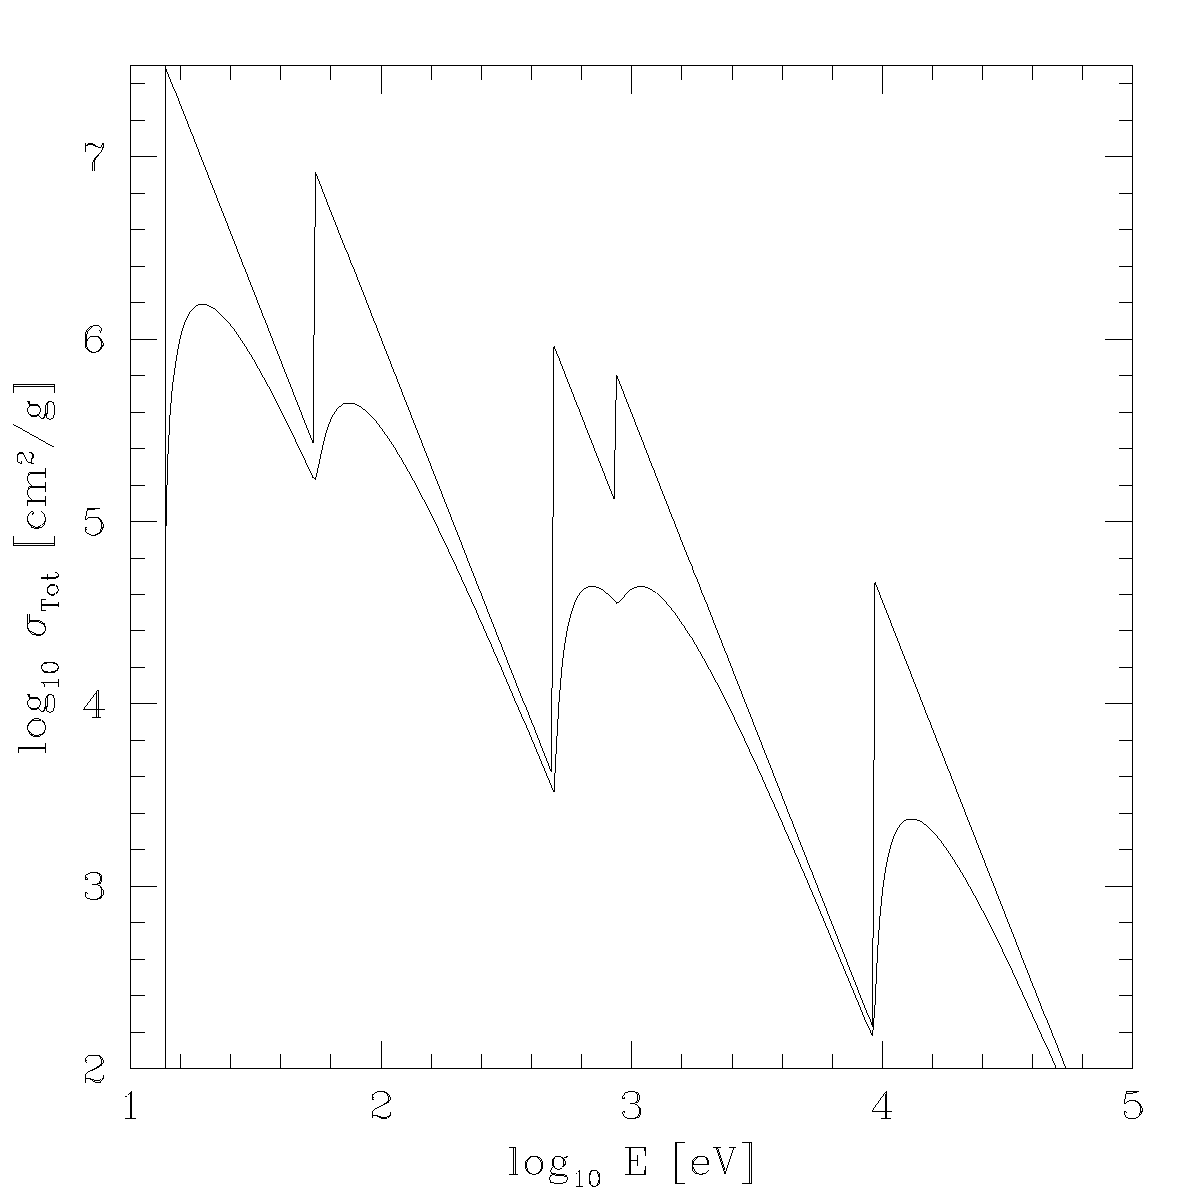
\includegraphics[width=0.9\textwidth]{week9cross} }
\end{enumerate}

\ifx\bookloaded\undefined
\end{document}
\end
\fi


\section{Chapter 10} 
\begin{enumerate}
\item{\bf The Number of Levels}

I fit a Morse function to the potential of  H$_2^+$.  The parameters
were
\begin{equation}
E_{n,0} = -0.065 \frac{e^2}{a_0}, B_n = 0.07 \frac{e^2}{a_0}, \beta_n
= 0.7 a_0^{-1}, R_0 = 2.5 a_0
\end{equation}
How many vibrational levels does H$_2^+$ have?   How many rotational
levels does each vibrational level typically have?

{\bf Answer:}

Let's first to the rotational levels.  When we increase the value
of the angular momentum from $L$ to $L+1$ and the energy of the
molecule decreases, we have reached the maximum value of $L$.  From
Eq.~(14) we have
\begin{equation}
4 \hbar^2 \frac{(L+1)^2}{k \mu_{AB} R_0^4} = 1
\end{equation}
so
\begin{equation}
L_\rmscr{max} = \left ( \frac{k \mu_{AB} R_0^4}{4 \hbar^2} \right )^{1/2} - 1
\end{equation}
We need to determine $k$.  This is related to the parameters that I
gave in the question, we know that $\omega^2 = k/\mu_{AB}$ and in the Morse
potential $\omega^2 = 2 \beta_n^2 B_n$ so
\begin{equation}
k = 2\beta_n^2 B_n 
\end{equation}
and
\begin{equation}
L_\rmscr{max} = \left ( \frac{2 \beta_n^2 B_n  \mu_{AB} R_0^4}{4 \hbar^2} \right )^{1/2} - 1
\end{equation}
I'm going to substitute the units for the various quantities into the
expression above
\begin{equation}
L_\rmscr{max} = \left ( \frac{\beta_n B_n e^2 m_p a_0 R_0^4}{4
  \hbar^2} \right )^{1/2} - 1 = \left ( \frac{\beta_n B_n m_p R_0^4}{4 m_e} \right )^{1/2} - 1 
\end{equation}
where I used $\mu_{AB}=m_p/2$ and $e^2 a_0=\hbar^2/m_e$.  The
expression in the parenthesis is dimensionless!  I get
\begin{equation}
L_\rmscr{max} = 23.79.
\end{equation}
Because $L$ ranges from zero to $L_\rmscr{max}$, I have 24 or 25
levels.

A formula for the number of vibrational levels is given explicitly in
Eq. (19).  The number of levels is
\begin{equation}
\frac{(2 \mu_{AB} B_n)^{1/2}}{\beta_n \hbar} + \frac{1}{2} = 
\frac{B_n^{1/2}}{\beta_n} \left ( m_p \frac{e^2}{a_0} a_0^2 \hbar^{-2}
\right )^{1/2}  + \frac{1}{2} = 
\frac{B_n^{1/2}}{\beta_n} \left ( \frac{m_p}{m_e} \right )^{1/2}  +
\frac{1}{2} = 16.7
\end{equation}

\item{\bf Nuclear Overlap}

Consider two deuterons bound by a single electron as in question (1).
What is the probability that the two deuterons lie on top of each
other, {\ie} that $R<4$~fermi, the diameter of the deuteron?   What is the
probability if the two deuterons are bound by a single muon, $m_\mu
\approx 207 m_e$?  You can find the eigenfunctions of the Morse
potential on Wikipedia.

If you assume that whenever the deuterons overlap they fuse and that
you get to ``roll the dice'' once each oscillation period, calculate
the fusion rate in both cases.

{\bf Answer:}
\index{muon-catalysed fusion}

The probability of overlap is simply the squared modulus of the
nuclear wavefunction evaluated at $r=0$ integrated over the volume
$4/3 \pi (4~\mathrm{fermi})^3$.  The nuclear wavefunction is given by
\begin{equation}
\Psi_n(z) = N_n z^{\lambda - n - \frac{1}{2}} e^{-z/2} L_n^{2\lambda-2n-1}(z)
\end{equation}
where $\lambda=\sqrt{2 M B_n}/(\beta_n \hbar)$ and the normalization
\begin{equation}
N_n=n! \left [ \frac{\beta_n (2\lambda - 2 n - 1)}{\Gamma(n+1)
    \Gamma(2\lambda - n)} \right]^{1/2} 
\end{equation}
and $L^{\alpha}_n$ is a Laguerre polynomial and $z=2\lambda
e^{-(x-x_e)}$ and $x=\beta_n r$.   This wavefunction is in terms of
$r$ as a one-dimensional coordinate; it is analogous to the function
$R(r)$ in the expansion of the atomic wavefunction in spherical
symmetry.   The complete wavefunction is
\begin{equation}
\psi(r,\theta,\phi) = \frac{1}{\sqrt{4\pi}} r^{-1} \Psi_0(z) ,
\end{equation}
so the probability of the two nuclei being within 4~fermi of each
other is given by
\begin{equation}
P = \int_0^{4~\mathrm{fermi}}  d r \left | \Psi \left (2 \lambda \exp
  \left [ \beta_n R_0 \right ] \right ) \right |^2 = \frac{4~\mathrm{fermi}}{a_0} \left | \Psi\left(2 \lambda \exp
  \left [ \beta_n R_0 \right ]\right) \right |^2
\end{equation}

Since we are interested in the ground state, $n=0$ so
\begin{equation}
L_n^{2\lambda-2n-1} = 1 ~\mathrm{and}~ N_n = \left [ \frac{\beta_n ( 2
    \lambda -1)}{\Gamma(2\lambda)} \right ]^{1/2} 
\end{equation}
which simplifies matters.  What remains is to calculate determine how
the value of $\lambda$ depends on the mass of the binding particle
muon or electron.  We have
\begin{equation}
\lambda = \frac{\sqrt{2 M A e^2/a_0}}{B a_0^{-1} \hbar} =
\frac{\sqrt{2 A}}{B} \sqrt{\frac{M}{m}}
\end{equation}
where $M$ is the reduced mass of the pair of deuterons and $m$ is the
mass of the muon or electron.  The constants $A$ and $B$ are simply
the numerical constants $0.07$ and $0.7$ that define the parameters of
the Morse potential in dimensionless units.  For the electronically bound
system $\lambda=22.9$ and for the muonically bound system
$\lambda=1.59$.

What remains is to evaluate the wavefunctions in both cases, for the
electron we have
\begin{equation}
\Psi(R=0) = 7.5 \times 10^{-30}
\end{equation}
and for the muon we have
\begin{equation}
\Psi(R=0) = 2.0 \times 10^{-3}.
\end{equation}
Converting these to probabilities yields 
\begin{equation}
P_\mathrm{electron} = 5 \times 10^{-63}, P_\mathrm{muon} = 6 \times 10^{-8}.
\end{equation}
To get a fusion rate we should multiply these by the typical frequency
of the systems say $\omega=2\beta_n^2 B_n/M=2 A B^2 e^2/(a_0^3 m_D/2)$
or $1.2 \times 10^{16}$~Hz for the electron and $3.6 \times
10^{19}$~Hz for the muon.  Therefore, we get a rate of three deuterium
fusions over the age of the universe in one ton of deuterium for
electronically bound molecules or $2 \times 10^{12}$~Hz for the
muonically bound molecule or about 4 million times over the 2.2$\mu$s
lifetime of the muon.  

It turns out that the rate-limiting step in muonic fusion is the
formation of muonic molecules which takes about one thousand times
longer than the fusion, but even this is not the killer.  It is the
fact that about one percent of the time the muon stays stuck to the
fusion product so cannot catalyse another reaction.  The first person
to consider muon-catalysed fusion was John David Jackson, and Eugene
Wigner suggested that ``alpha sticking'' could be a problem.  This
process was the original ``cold fusion,'' and it almost breaks even
(within a factor of a few).
\index{cold fusion}
\end{enumerate}

%%% Local Variables: 
%%% mode: latex
%%% TeX-master: "book"

\ifx\bookloaded\undefined
\documentclass{article}
\ifx\pdftexversion\undefined
  \usepackage[dvips]{graphicx}
\else
  \usepackage[pdftex]{graphicx}
\fi
\newcommand{\be}{\begin{equation}}
\newcommand{\ee}{\end{equation}}
\newcommand{\rmmat}[1]{\hbox{\rm #1}}
\newcommand{\rmscr}[1]{{\hbox{\rm \scriptsize #1}}}
\newcommand{\comment}[1]{\relax}
\newcommand{\dd}[2]{\frac{d {#1}}{d {#2}}}
\newcommand{\pp}[2]{\frac{\partial {#1}}{\partial {#2}}}
\begin{document}
\fi

\section{Chapter 11}
\begin{enumerate}
 
\item{\bf Maximum Flux}

Calculate from the Euler equation and the continuity equation, at what
velocity does the flux ($\rho V$) reach its maximum for fluid flowing 
through a tube of variable cross-sectional area?   
At which velocities does the flux vanish?  You can consider the flow
to be adiabatic.

{\bf Answer:}

From Euler's equation we have
\begin{equation}
({\bf v} \cdot \nabla ){\bf v}=-\frac{\nabla P}{\rho}
\end{equation}
so
\begin{equation}
v \dd{v}{x} = -\frac{1}{\rho} \dd{P}{x}
\end{equation}
and we have
\begin{equation}
\dd{P}{\rho} = c_s^2
\end{equation}
Combining these two gives
\begin{equation}
\dd{\rho}{v} = -\rho \frac{v}{c_s^2}
\end{equation}
We have
\begin{equation}
\dd{(\rho v)}{v} = \rho + v \dd{\rho}{v} = \rho \left ( 1  -
\frac{v^2}{c_s^2} \right )
\end{equation}
This function reaches an extremum at $v=c_s$.  Because the flux is
zero for $v=0$ and increases with $v$ for $v \ll c_s$, this must be a
maximum for $jv$.

If we assume that the sound speed is constant (isothermal gas), 
this integrates to give
\begin{equation}
\rho v = \rho_0 v e^{-v^2/(2c_s^2)}
\end{equation}
where $\rho_0$ is the density at zero velocity.  This has a maximum of
$\rho_0 c e^{-1/2}$ at
$v=c_s$.  We can let the gas expand and accelerate to arbitrarily high
velocities.   In a more realistic situation, the sound speed is a
function of density
\begin{equation}
c_s^2 = c_{s,0}^2 \left ( \frac{\rho}{\rho_0} \right )^{\gamma-1},
\end{equation}
and we have 
\begin{equation}
\dd{j}{v} = \rho \left [ 1  -
\frac{v^2}{c_{s,0}^2} \left ( \frac{\rho}{\rho_0} \right )^{1-\gamma} \right ]
 = \frac{j}{v} \left [ 1  -
\frac{v^2}{c_{s,0}^2} (\rho_0 v)^{\gamma-1} j^{1-\gamma} \right ]
\end{equation}
with $j=\rho v$.  This differential equation has the following
solution
\begin{equation}
j(v) = \rho_0 v \left [ 1 + \left ( 1 - \gamma \right )
  \frac{v^2}{2 c_{s,0}^2} \right ]^{1/(\gamma-1)}
\end{equation}
If we take $\gamma\rightarrow 1$ we get the solution above for the
isothermal case.  The flux reaches a maximum of
\begin{equation}
j_\mathrm{max} = \rho_0 c_{s,0} \left ( \frac{2^\gamma}{\gamma+1}
\right )^{1/(\gamma-1)} \frac{1}{\sqrt{2\gamma+2}}
\end{equation}
at a velocity of
\begin{equation}
  v = \sqrt{\frac{2}{\gamma+1}} c_{s,0}.
\end{equation}
Unlike the isothermal case, the flux vanishes at
$v=0$ and $v=c_{s,0}\sqrt{2/(\gamma-1)}$.  How can we understand this
second velocity when the flux vanishes?   Along a streamline of the
gas we have
\begin{equation}
\frac{v^2}{2} + w = w_0 = \frac{P + \epsilon}{\rho} = \frac{P +
  (\gamma-1)^{-1} P}{\rho} = \frac{\gamma}{\gamma-1} \gamma^{-1} c_{s,0}^2
\end{equation}
The maximum velocity that the gas can attain is
\begin{equation}
v = \sqrt{2 w_0} = \sqrt{2 c_{s,0}^2/(\gamma-1)} = c_{s,0} \sqrt{2/(\gamma-1)}
\end{equation}
% Since we have a solution for $j(v)$, it would be nice to find the
% velocity at which the momentum flux is maximized for a given mass
% flux.   The momentum flux is
% \begin{equation}
% f(v) = P + \rho v^2 = P + j(v) v = \frac{c_s^2 \rho}{\gamma} + j(v) v
% = \frac{c_s^2 j(v)}{v \gamma} + j(v) v
% \end{equation}
% Let's take
% \begin{equation}
% \left . \dd{f}{v}\right|_{j(v)} = j(v) \left [ \frac{1}{\gamma} \left
%     ( \left(\gamma-1\right ) \frac{c_s^2}{\rho v} \left (-\rho
%       \frac{v}{c_s^2}\right ) - \frac{c_s^2}{v^2} \right ) + 1 \right ]
% \end{equation}
% \begin{equation}
% \left . \dd{f}{v}\right|_{j(v)} = j(v) \left [ 1 - \frac{\gamma-1 +
%     \frac{c_s^2}{v^2}}{\gamma} \right ]
% \end{equation}
% so
% \begin{equation}
% v = c_s.
% \end{equation}

% The maximum momentum flux as a function of velocity (not for fixed mass
% flux) occurs at a different velocity.  We have
% \begin{equation}
% f(v) = \frac{c_s^2 \rho}{\gamma} - \rho v^2
% \end{equation}
% so
% \begin{equation}
% \dd{f}{v} = \left ( \frac{\gamma-1}{\gamma} c_s^2 + \frac{1}{\gamma}
%   c_s^2 \right - v^2) \left ( -\rho \frac{v}{c_s^2} \right )  - 2 v \rho= \rho v \left
%   (3-\frac{v^2}{c_s^2}\right )
% \end{equation}
% and the maximum occurs at $v=\sqrt{3} c_s$.

\item{\bf Stream Bed}

  Fig.~\ref{fig:channel} shows how the level of the surface changes
  for a flow passing over an obstacle.  For an initial depth of
  $z_0=1$ and $g=10$ and a bump height of $y(x)=0.1 e^{-x^2}$, find the
  solutions to Bernoulli's equation (Eq.~\ref{eq:bern}) for $z$ as a
  function of $x$ and the initial velocity $v_0$.  You may find
  several solutions for a given $x$.   Also you should only worry
  about the positive real solutions for $z$.  What are the values of
  the critical velocities $v_0$?

{\bf Answer:}

The solution follows from Eq.~\ref{eq:675} by plugging in the values
of $y(x)$, $z_0=1$, $g=10$ and $v_0$ which you are going to vary to look
at the different solutions.  This yields
\begin{equation}
A = \frac{v_0^2}{2}, B=\frac{v_0^2}{2} + 10 \left [ 1 - 0.1 e^{-x^2}
  \right ], C = 10.
\end{equation}
Next we use Eq.~\ref{eq:cubic_sol} to find the value of $\cos 3 t$.
This equation will yield several values of $3t$ because the cosine
function is symmetric and periodic.  They are
\begin{equation}
3 t = 3 t_1, 3 \left (-t_1 \right ), 
3 \left ( t_1 + \frac{2}{3} \pi \right ), 
3 \left ( \frac{2}{3} \pi - t_1 \right ),
3 \left ( t_1 + \frac{4}{3} \pi \right ), 
3 \left ( \frac{4}{3} \pi - t_1 \right ).
\end{equation}
Because we are interested in the value of $\cos t$, the first two
results yield the same value.  Let's draw a picture with the various
possibilities numbered:

\newcommand{\circlepic}[2]{
\begin{tikzpicture}
\draw (0,0) circle (#2) 
      (0,0) -- ++(#1:#2) node {1} 
      (0,0) -- ++(-#1:#2) node {2}
      (0,0) -- ++(120+#1:#2) node {3}
      (0,0) -- ++(120-#1:#2)  node {4}
      (0,0) -- ++(240+#1:#2) node {5}
      (0,0) -- ++(240-#1:#2) node {6} ; 
\end{tikzpicture}
}
\circlepic{25}{1.5} \circlepic{35}{1.5} \circlepic{60}{1.5}

Because we are only interested in the $x-$coordinate (the cosine of
the angle), we see that solutions 1 and 2, 3 and 6 and 4 and 5 are
equivalent, so we only need to keep the solutions with $t$ between
zero and $\pi$.  In the left diagram we used $t=25^\circ$ so we only have
a single value with $\cos t$ greater than zero. We can discard
negative values of $\cos t$ because that would yield that the surface
of the water lies underneath the surface of the bottom.

For $t_1>30^\circ$ there are two positive solutions.  The centre
diagram has $t_1=35^\circ$. These solutions coincide for
$t_1=60^\circ$ (right diagram).  Where this condition holds the flow
is travelling at the critical velocity.  The value of $v_0$ that
causes the flow to travel at the critical velocity over the peak of
the bump is the critical value of $v_0$.   In general, we only have to
be concerned with solutions (1) and (4), the rest are repeats or
negative.

\item{\bf Sound Velocity}

  Show that for a linear sound wave {\em i.e.} one in which $\delta
  \rho \ll \rho$ that the velocity $v$ of fluid motion is much less
  than $c_s$. Estimate the maximum longitudinal fluid velocity in the
  case of a sound wave in air at STP in the case of a disturbance
  which sets up pressure fluctuations of order 0.1\%.

{\bf Answer:}

Starting with Eq.~\ref{eq:660} we can relate the velocity of the fluid
in the wave to the pressure disturbance,
\begin{equation}
{\bf v}' = \frac{p'}{\rho_0} \frac{{\bf k} }{\omega}, v' =
\frac{p'}{\rho_0} \frac{1}{c_s} = c_s \frac{\rho'}{\rho_0} =
\frac{p'}{p_0} \frac{c_s}{\gamma}
\end{equation}
where $p' = c_s^2 \rho'$ because $c_s^2=\partial p/\partial \rho$.
Furthermore, the adiabatic exponent is given by $\gamma=\partial \ln
p/\partial \ln \rho=(\rho/p) c_s^2$.

\end{enumerate}

\ifx\bookloaded\undefined
\end{document}
\end
\fi
%%% Local Variables:
%%% TeX-master: "book"
%%% End:
\ifx\bookloaded\undefined
\documentclass{article}
\ifx\pdftexversion\undefined
  \usepackage[dvips]{graphicx}
\else
  \usepackage[pdftex]{graphicx}
\fi
\newcommand{\be}{\begin{equation}}
\newcommand{\ee}{\end{equation}}
\newcommand{\rmmat}[1]{\hbox{\rm #1}}
\newcommand{\rmscr}[1]{{\hbox{\rm \scriptsize #1}}}
\newcommand{\comment}[1]{\relax}
\newcommand{\dd}[2]{\frac{d {#1}}{d {#2}}}
\newcommand{\pp}[2]{\frac{\partial {#1}}{\partial {#2}}}
\begin{document}
\fi

\section{Chapter 12}
\begin{enumerate}
\item{\bf Shock Entropy}
  Show that the entropy of the fluid increases as it passes
  through a shock. Hint: the equation of state of an isentropic fluid
  is $P = K\rho^\gamma$ where the value of $K$ increases with
  increasing entropy.

{\bf Answer:}

The simplest way to solve this is to look at the shock adiabat and see
that the entropy increases along it, but let's be a bit more
rigorous.  The value of $K$ is a function of entropy alone, so let's
look at how $K$ changes across the shock.   Specifically what is
$P/\rho^\gamma$ on each side of the shock?  We have
\begin{equation}
\frac{\rho_2}{\rho_1} = \frac{(\gamma+1)
  M_1^2}{2 + M_1^2 (\gamma-1)},
\frac{P_2}{P_1} = \frac{1-\gamma + 2 M_1^2 \gamma }{(\gamma+1)}
 \end{equation}
so 
\begin{equation}
\frac{K_2}{K_1} = \frac{1-\gamma + 2 M_1^2 \gamma }{(\gamma+1)} 
\left [ \frac{(\gamma+1)
  M_1^2}{2 + M_1^2 (\gamma-1)} \right ]^{-\gamma}
\end{equation}
Let's expand this ratio for $M_1^2 \approx 1$ to understand the change
in entropy for a weak shock,
\begin{equation}
\frac{K_2}{K_1} = 1 + \frac{2\gamma(\gamma-1)}{3(\gamma+1)^2} \left (M_1^2 - 1\right
)^3 + {\cal O} \left (M_1^2 - 1\right)^4.
\end{equation}
The value of $K$ increases across the shock for $\gamma>1$, therefore
the entropy increases.  To make this precise we know that for an ideal
gas, $s = c_V \ln K + s_0$, so 
\begin{equation}
\Delta s = c_v \frac{\Delta K}{K} =
\frac{2\gamma(\gamma-1)}{3(\gamma+1)^2} \left (M_1^2 - 1\right )^3 c_V
+ + {\cal O} \left (M_1^2 - 1\right)^4.
\end{equation}

\item{\bf Bomb Yield}

  Fig.~\ref{fig:tumbler} shows shocked air heated to incandescence
  about two milliseconds after the detonation of a nuclear
  bomb.  The height of the device was 90~meters.  What
  was the approximate yield of the device?

{\bf Answer: }

Eq.~\ref{eq:710}.

\item{\bf Relativistic Shock}

  Find the incoming and outgoing velocity of a relativistic shock in
  terms of the energy density and pressure on either side of the
  shock.

{\bf Answer:}

Start with Eq.~\ref{eq:855} and~\ref{eq:856},
\begin{equation}
 w_1 U_1 \gamma_1= w_2 U_2 \gamma_2, w_1 U_1^2 + p_1 = w_2 U_2^2 + p_2.
\end{equation}
Let's use the second equation to solve for $U_2^2$
\begin{equation}
U_2^2 = \frac{w_1 U_1^2 + p_1 - p_2}{w_2} 
\end{equation}
and rewrite $\gamma_2^2$ in terms of $U_2$
\begin{equation}
\gamma_2^2 = \frac{1}{1-\beta^2} = \frac{\beta^2 + 1 -
  \beta^2}{1-\beta^2} = U_2^2 + 1.
\end{equation}
The square of the first equation yields
\begin{eqnarray}
w_1^2 U_1^2 \left ( U_1^2 + 1 \right ) &=& w_2^2 U_2^2 \left ( U_2^2 +
  1 \right ) \\
w_1^2 U_1^2 \left ( U_1^2 + 1 \right ) &=& w_2^2 \frac{w_1 U_1^2 + p_1 -
  p_2}{w_2} \left ( \frac{w_1 U_1^2 + p_1 - p_2}{w_2}  + 1 \right ) \\
U_1^2 &=& \frac{(p_1-p_2)^2 - p_1 w_2 - p_2 w_2}{w_1 \left [ w_2 - w_1
    + 2 ( p_1 - p_2 ) \right ]} \\
\left ( \frac{v_1}{c} \right )^2 &=&
\frac{(p_1-p_2)(p_1-p_2+w_2)}{(p_1-p_2-w_1)(p_1-p_2+w_2-w_1)} \\
\left ( \frac{v_1}{c} \right )^2 &=&
\frac{(p_2-p_1)(\epsilon_2+p_1)}{(\epsilon_2-\epsilon_1)(\epsilon_1+p_2)} 
\end{eqnarray}
and we obtain $v_2$ by swapping the one and two indicies in the
previous equaiton, yielding 
\begin{eqnarray}
\frac{v_1}{c} &=&
\sqrt{\frac{(p_2-p_1)(\epsilon_2+p_1)}{(\epsilon_2-\epsilon_1)(\epsilon_1+p_2)}} \\
\frac{v_2}{c} &=&
\sqrt{\frac{(p_2-p_1)(\epsilon_1+p_2)}{(\epsilon_2-\epsilon_1)(\epsilon_2+p_1)}} 
\end{eqnarray}

\item{\bf Relativistic Bernoulli}

  Find the relativistic generalisation of Bernoulli's equation for a
  streamline (you can neglect gravitiy).

{\bf Answer:}

For the Bernoulli equaion we must assume that all time derivatives
vanish and look at the properties of the fluid along a flow line.  We
can use the shock jump conditions as a starting point,
(e.g. Eq.~\ref{eq:854} and~\ref{eq:855}), because they must hold along
a streamline as well as across a discontinuity.  We have 
\begin{equation}
U n = \textrm{constant}, w U \gamma =  \textrm{constant}.
\end{equation}
Using the first equation to eliminate $U$ from the second yields
\begin{equation}
\frac{\gamma w}{n} = \textrm{constant}.
\end{equation}
This doesn't look much like the non-relativistic Bernoulli equation.
Let's make some substitutions.  We have
\begin{equation}
\frac{1}{n} \left ( 1 + \frac{v^2}{2 c^2}\right ) \left ( \rho c^2 + w_{NR,V}
\right ) + \textrm{Higher order in velocity} = \textrm{constant}.
\end{equation}
Now let's divide both sides by the rest mass of the particles 
\begin{equation}
\frac{1}{\rho} \left ( 1 + \frac{v^2}{2 c^2}\right ) \left ( \rho c^2 + w_{NR,V}
\right ) + \textrm{Higher order in velocity} = \textrm{constant}
\end{equation}
and expand, dropping higher-order terms
\begin{equation}
c^2 + \frac{v^2}{2} + \frac{w_{NR,V}}{\rho}  = \textrm{constant}
\end{equation}
and
\begin{equation}
\frac{v^2}{2} + w  = \textrm{constant}
\end{equation}
where $w$ is the enthalpy per unit mass.  This is the non-relativistic
Bernoulli equation.  For the classical result with an incompressible fluid
we have $w=P/\rho$.

\item{\bf Bathtub Physics}

  When water flows into a bathtub, a circular hydraulic jump forms
  around the incoming stream of water.  If you assume that the flow
  rate is constant and the flow is initially vertical, calculate the
  height of the water downstream of the jump as a function of the
  radius of the jump and the flow rate.  You may neglect friction. If
  the bathtub is large compared to the radius of the jump and the
  walls are vertical, how does the radius of the jump change with
  time?

{\bf Answer:}

Here the flow rate and downstream height are given.  We have
\begin{equation}
  j = \frac{Q}{2 \pi r}
\end{equation}
where $Q$ is the volumetric flow rate and $r$ is the radius of the
jump.  What is the height of the upsteam flow $h_1$ in terms of the
downstream height $h_2$?  We have
\begin{equation}
v_1^2 h_1 + \frac{1}{2} g h_1^2 = v_2^2 h_2 + \frac{1}{2} g h_2^2
\end{equation}
so
\begin{equation}
\frac{j^2}{h_1} + \frac{1}{2} g h_1^2 = \frac{j^2}{h_2} + \frac{1}{2} g h_2^2
\end{equation}
and with rearranging
\begin{equation}
j^2 \left ( h_1 - h_2 \right ) + \frac{1}{2} g \left ( h_2^3 h_1 -
  h_1^3 h_2 \right ) = 0.
\end{equation}
We can factor this to give
\begin{equation}
\frac{1}{2} \left( h_1 - h_2 \right ) \left ( g h_2 h_1^2  + g h_2^2 h_1 - 2
    j_2 \right ) = 0
\end{equation}
so we have the positive solutions
\begin{equation}
h_1 = h_2, h_1 = \frac{h_2}{2} \left ( \sqrt{ 1 + \frac{8 j^2}{g
      h_2^3}} - 1 \right ).
\end{equation}
Now we use that $v_1$ is constant to eliminate $h_1=j/v_1=Q/(2\pi r
v_1)$.  Furthermore, $h_2=Q t/A$ where $A$ is the cross-sectional area
of the jump.  Putting all of these into the equation above yields
\begin{equation}
\frac{Q}{2\pi r v_1} = \frac{Q t}{2 A} \left ( \sqrt{ 1 + 
\frac{8}{g} \left (\frac{Q}{2\pi r} \right )^2 \left ( \frac{A}{Q t} \right)^3
} - 1 \right ).
\end{equation}
and solving for the radius $r$ yields
\begin{equation}
r = \frac{A \left ( 2 A v_1^2 - t Q g \right )}{2 \pi t^2 Q g  v_1} 
= \frac{A^2 v_1}{Q g \pi} \frac{1}{t^2} - \frac{A}{2\pi v_1} \frac{1}{t}.
\end{equation}
\end{enumerate}

\ifx\bookloaded\undefined
\end{document}
\end
\fi
%%% Local Variables:
%%% TeX-master: "book"
%%% End:
\ifx\bookloaded\undefined
\documentclass{article}
\ifx\pdftexversion\undefined
  \usepackage[dvips]{graphicx}
\else
  \usepackage[pdftex]{graphicx}
\fi
\newcommand{\be}{\begin{equation}}
\newcommand{\ee}{\end{equation}}
\newcommand{\rmmat}[1]{\hbox{\rm #1}}
\newcommand{\rmscr}[1]{{\hbox{\rm \scriptsize #1}}}
\newcommand{\comment}[1]{\relax}
\newcommand{\dd}[2]{\frac{d {#1}}{d {#2}}}
\newcommand{\pp}[2]{\frac{\partial {#1}}{\partial {#2}}}
\begin{document}
\fi

\section{Chapter 13}
\begin{enumerate}
\item{\bf Exact Solutions}

For which values of $\gamma$ can the Bernoulli equation
(Eq.~\ref{eq:725}) be solved using elementary methods (linear,
quadratic and cubic equations of the form in Eq.~\ref{eq:676}).  There
are many, however only a few have $1< \gamma < 5/3$.

{\bf Answer: }

Let's start with the Bernoulli equation,
\begin{equation}
\frac{v^2}{2} + \frac{c_s^2 - c_s^2(\infty)}{\gamma - 1} - \frac{G M}{r} = 0.
\end{equation}
First let's divide both sides by $c_s^2$ to get
\begin{equation}
\frac{1}{2} \frac{v^2}{c_s^2} + \frac{1 - c_s^2(\infty)/c_s^2}{\gamma -
  1} - \frac{G M}{r c_s^2} =
\frac{1}{2} \frac{v^2}{c_s^2} + \frac{1 - c_s^2(\infty)/c_s^2}{\gamma -
  1} - \frac{r_c}{r} \frac{4}{5-3\gamma} \frac{c_s^2(\infty)}{c_s^2} = 0.
\end{equation}
We need to express the sound speed in terms of $r$ and $v$.  We have
\begin{equation}
P = K \rho^\gamma
\end{equation}
so
\begin{equation}
c_s^2 = \gamma K \rho^{\gamma-1} = c_s^2(\infty) \left ( \frac
{\rho}{\rho(\infty)} \right )^{\gamma - 1}
\end{equation}
We can relate $v$, $r$ and $\rho$ through ${\dot M}=4\pi r^2 v \rho$
We are interested in a plot of $y=v/c_s$ versus $x=r/r_c$, so let's
substitute for $x$ and $y$ to get
\begin{equation}
\frac{y^2}{2} + \frac{1}{\gamma-1} - \left ( \frac{1}{\gamma-1}  - \frac{1}{x}
\frac{4}{5-3\gamma} \right ) \frac{c_s^2(\infty)}{c_s^2} = 0.
\end{equation}
Now we need to find $c_s^2(\infty)/c_s^2$ in terms of $x$ and $y$.  We
can determine $\rho$ at any point through ${\dot M}=4\pi \rho v$ and 
the formula above.  
The key is to write ${\dot M}=\alpha {\dot M}_\rmscr{crit}$.  First,
we have
\begin{equation}
\dot M = 4 \pi r^2 v \rho = 4 \pi \alpha r_c^2 c_s(r_c) \rho(r_c)
\end{equation}
so
\begin{equation}
\frac{\rho}{\rho(r_c)} = \frac{\alpha}{x^2 y} \frac{c_s(r_c)}{c_s}
= \frac{\alpha}{x^2 y} \left (
  \frac{\rho(r_c)}{\rho} \right )^{(\gamma-1)/2} = \left ( \frac{\alpha}{x^2 y} \right )^{2/(\gamma+1)}\kern-0.5cm.
\end{equation}
and
\begin{equation}
\frac{\rho}{\rho(\infty)} = \frac{\rho}{\rho(r_c)}
\frac{\rho(r_c)}{\rho(\infty)}
= \left ( \frac{\alpha}{x^2 y} \right )^{2/(\gamma+1)} \left ( \frac{2}{5-3\gamma} \right )^{1/(\gamma-1)}
\end{equation}
using Eq.~\ref{eq:729} and giving an expression for
\begin{equation}
\frac{c_s^2}{c_s^2(\infty)} = \left ( \frac{\alpha}{x^2 y} \right )^{2(\gamma-1)/(\gamma+1)}  \frac{2}{5-3\gamma} 
\end{equation}
Let's substitute this into the Bernoulli equation to yield
\begin{eqnarray}
 y^{2(1-\gamma)/(\gamma+1)} \left ( \frac{y^2}{2} + \frac{1}{\gamma-1}
 \right ) \frac{2 \alpha^{2(\gamma-1)/(\gamma+1)}}{5 -3\gamma} -
 \nonumber \\
x^{4(\gamma-1)/(\gamma+1)}\left ( \frac{1}{\gamma-1}  
+ \frac{4}{x(5 - 3\gamma)} \right )
=0
\label{eq:789}
\end{eqnarray}
There could be many possibilities: we could solve for $x$ or $y$ in
terms of the other, and the resulting equation could be a cubic,
quadratic or linear in the three terms.  Let's begin with solving for
$x$.

{\bf Solution for $x$:}

On the second line there are two terms in $x$ that differ by a
single power of $x$.  We can make substitutions of the form $x=u^{\pm 2}$,
$x=w^{\pm 3}$ that will transform the equation into a quadratic or cubic
with the correct choice of $\gamma$, or we could solve for $x$ directly
which would require that $4(\gamma-1)/(\gamma+1)=2,1,0,-1,-2$,
yielding quadratic, linear, linear, quadratic and cubic equations,
respectives.  A value of $4(\gamma-1)/(\gamma-1)=3$ would also yield a
cubic equation but not of the simply solvable form
(Eq.~\ref{eq:676}).  There are also simply solvable quartics, but this
is beyond the scope of the question.
\begin{table}[h]
\centering
\begin{tabular}{ccccc}
$\frac{4(\gamma-1)}{\gamma-1}$ & $\gamma$ & Type & Substitution & Comment \\ \hline
2 & 3 & quadratic & $x$ & Non-Ideal \\
1 & $5/3$ & linear & $x$ & Divergent \\
0 & 1 & linear & $x$ & Divergent \\
$-1$ & $3/5$ & quadratic & $x$ & Unphysical\\
$-2$ & $1/3$ & cubic & $x$ & Unphysical \\
$1/2$  & $9/7$ & quadratic & $x=u^2$ & Good \\
$-1/2$ & $7/9$ & cubic & $x=u^{-2}$ & Unphysical  \\
$2/3$ & $7/5$ & cubic & $x=w^3$ & Good \\
$1/3$ & $13/11$ & cubic & $x=w^{-3}$ & Good \\
\end{tabular} 
\end{table}

{\bf Solution for $y$:}

We can also solve for $y$ in terms of $x$.  Here the two terms in $y$
differ by two powers of $y$; this naturally leads to a quadratic
without substitution.  Some of the various possibilities are listed in
the following table.
\begin{table}[h]
\centering
\begin{tabular}{ccccc}
$\frac{2(1-\gamma)}{\gamma+1}$ & $\gamma$ & Type & Substitution &
Comment \\ \hline
2 & 0 & quadratic & $w=y^2$ & Unphysical \\
1 & $1/3$ & cubic & $y$ & Unphysical \\
0 & 1 & linear & $w=y^2$ & Divergent \\
$-2/3$ & 2 & cubic & $w^3=y^2$ & Non-Ideal \\
-1 & 3 & quadratic & $y$ & Non-Ideal \\
$-4/3$ & 5 & cubic & $w^{-3}=y^2$ & Non-Ideal \\
\end{tabular} 
\end{table}

\setcounter{enumi}{3}
\item{\bf Bondi Solution}

Generate a picture like the figure in the lecture notes for the Bondi
solution to spherical accretion.  Use $\gamma=9/7$.

{\bf Answer: }

The answer starts as the first question up to the Bernoulli equation
(Eq.~\ref{eq:789}) where we substitute $\gamma=9/7$ to yield

\begin{equation}
\frac{7}{2} x^{1/2} - \frac{7}{2} x^{-1/2} - \frac{7}{8} \alpha^{1/4}
y^{7/4} - \frac{49}{8} \frac{\alpha^{1/4}}{y^{7/4}} = 0
\end{equation}
Let $u=\sqrt{x}$ and multiply everything by $u$ to give a quadratic
equation for $u$
\begin{equation}
\frac{7}{2} u^2 - \left [ \frac{7}{8} \frac{\alpha^{1/4}}{y^{1/4}}
  (y^2 + 7 ) \right ]u -
\frac{7}{2} = 0
\end{equation}

\item{\bf Bondi Solution --- Harder}

Generate a picture like the figure in the lecture notes for the Bondi
solution to spherical accretion.  Use $\gamma=7/5$.

{\bf Answer: }

The answer starts as the first question up to the Bernoulli equation
(Eq.~\ref{eq:789}) where we substitute $\gamma=7/5$ to yield
\begin{equation}
\frac{5}{2} x^{2/3} - 5 x^{-1/3} - \frac{5}{4} \alpha^{1/3} y^{5/3} -
\frac{25}{4} \frac{\alpha^{1/3}}{y^{1/3}} = 0.
\end{equation}
Let $w^3=x$ and multiply everything by $u$ to give a cubic
equation for $w$
\begin{equation}
\frac{5}{2} w^3 - \frac{5}{4} \frac{\alpha^{1/3}}{y^{1/3}} \left ( y^2
  - 5 \right ) w - 5= 0.
\end{equation}
of the form Eq.~\ref{eq:676}.  This equation can be solved analytically

\item{\bf Accretion Energetics}

\begin{enumerate}
\item $T=\frac{G M m}{R}$
\item $T=\frac{G M m}{2 R}$
\item $T_\textrm{\scriptsize NS}/m=2 \times 10^{20}$ erg/g,
  $T_\textrm{\scriptsize WD}/m=8
  \times 10^{16}$ erg/g. The accretion energy for a neutron star
  greatly exceeds the nuclear energy.  The opposite holds for a white
  dwarf.
\item The total energy per gram is essentially the value given in part
  c).  The Eddington luminosity is $1.8\times 10^{38}$~erg/s for a
  neutron star (see problem 3.6).  This yields an Eddington accretion
  rate of approximately $10^{18}$~g/s. 
\end{enumerate}

\item{\bf A simplified accretion disk}

\begin{enumerate}
\item $dE = -\frac{G M dm}{2 r}$
\item $\frac{d}{dr} dE = \frac{G M dm}{2 r^2}$, $\frac{dE}{dr dt}=
  \frac{GM}{2 r^2} \frac{dm}{dt}$
\item $\frac{dE}{dA dt}= \frac{GM}{4 \pi r^3} \frac{dm}{dt}$
\item $\sigma T^4 =  \frac{GM}{4 \pi r^3} \frac{dm}{dt}$
\item $\frac{dE}{dt} = \int_{r_0}^{r_A}   \frac{GM}{2 r^2}
  \frac{dm}{dt} dr = \frac{GM}{2} \frac{dm}{dt} \left ( r_0^{-1} -
    r_A^{-1} \right )$, the peak temperature is at $r_0$ and the
  minimum temperature is at $r_A$.
\item To sketch the spectrum we will assume that the BB emission
  emerges exclusively at the peak of the BB, so we need to translate
  $dE/(dr dt)$ to $dE/(dT dt)$.
$$
\frac{dP}{dT} = \frac{dP}{dr} \frac{dr}{dT} = 
  \frac{GM}{2 r^2} \frac{dm}{dt} \left ( \frac{\sigma T^3 4 \pi r^4}{3
      G M {\dot m}} \right ) = \frac{4 \pi r^2 \sigma T^3}{3}
$$
and substituting yields
$$
\frac{dP}{dT} = \frac{4\pi \sigma}{3} \left ( \frac{G M}{4\pi \sigma}
  {\dot m} \right )^{2/3} T^{1/3}
$$
or $F_\nu \propto \nu^{1/3}$.
\item If the accretion rate exceeds the Eddington rate, some matter
  must be expelled.
\item Viscosity
\end{enumerate}
\end{enumerate}

\ifx\bookloaded\undefined
\end{document}
\end
\fi

%%% Local Variables:
%%% TeX-master: "book"
%%% End:
\ifx\bookloaded\undefined
\documentclass{article}
\ifx\pdftexversion\undefined
  \usepackage[dvips]{graphicx}
\else
  \usepackage[pdftex]{graphicx}
\fi
\newcommand{\be}{\begin{equation}}
\newcommand{\ee}{\end{equation}}
\newcommand{\rmmat}[1]{\hbox{\rm #1}}
\newcommand{\rmscr}[1]{{\hbox{\rm \scriptsize #1}}}
\newcommand{\comment}[1]{\relax}
\newcommand{\dd}[2]{\frac{d {#1}}{d {#2}}}
\newcommand{\pp}[2]{\frac{\partial {#1}}{\partial {#2}}}
\begin{document}
\fi

\section{Chapter 14}
\begin{enumerate}
\item{\bf X-ray Bursts:}

We will try to model Type-I X-ray bursts using a simple model for the instability. We will calculate how much material will accumulate on a neutron star before it bursts.
\begin{enumerate}
\item Let us assume that the star accretes pure helium, that the
  temperature of the degenerate layer is constant down to the core
  ($T_c$), how much luminosity emerges from the surface of the star? 

\item Let us assume that the helium layer has a mass, $dM$, and that the enregy generation rate for helium burning is given by
$$
\epsilon_{3\alpha} = 3.5 \times 10^{20} T_9^{-3} \exp(-4.32/T_9) \mathrm{erg s}^{-1} \mathrm{g}^{-1}
$$
where $T_9=T/10^9 \mathrm{K}$. The energy generation rate is a
function of density too, but let's forget about that to keep things
simple. How much power does the helium layer generate as a function of
$dM$?

\item Equate your answer to (a) to the answer to (b) and solve for
  $dM$. This is the thickness of a layer in thermal equilibrium.

\item Let's assume that the potential burst starts by the temperature
  in the accreted layer jiggling up by a wee bit. If the surface
  luminosity increases faster with temperature than the helium burning
  rate, then the layer is stable. Calculate $dL_\mathrm{surface}/dT$ and
  $dP_\mathrm{helium}/dT$.

\item Calculate the value of $dM$ for which $dP_\mathrm{helium}/dT$
  exceeds $dL_\mathrm{surface}/dT$ and the layer bursts.

\item Equate your value of $dM$ in (c) and (e) and solve for $T$. What
  is $dM$? How long will it take for such a layer to accumulate if the
  star is accreting at one-tenth of the Eddington accretion rate?

\end{enumerate}
{\bf Answer:}
\begin{enumerate}
\item If you assume free-free opacity you get using results from
  Chapter 1
$$
L_{\gamma,ff} = 2.35 \times 10^{8} \textrm{erg/s} \left (
  \frac{T}{1\textrm{K}}\right )^{7/2}
$$
or if you used the black-body formula you get
$$
L_{\gamma,BB} = 7 \times 10^{8} \textrm{erg/s} \left (
  \frac{T}{1\textrm{K}}\right )^4
$$
\item
$$
P_\textrm{\scriptsize He} = \epsilon_{3\alpha} dM =
3.5 \times 10^{20} T_9^{-3} \exp(-4.32/T_9) \mathrm{erg s}^{-1}
\mathrm{g}^{-1} dM
$$
\item 
$$
dM_{ff} = 2.12 \times 10^{19} T_9^{13/2} \exp (4.32/T_9) \textrm{g}
$$
and 
$$
dM_{BB} = 2 \times 10^{24} T_9^{7} \exp (4.32/T_9) \textrm{g}
$$
\item
$$
\frac{dL_{\gamma,ff}}{dT} = 8.2 \times 10^8 \textrm{erg/s/K} \left (
  \frac{T}{1\textrm{K}} \right)^{5/2}
$$
and
$$
\frac{dL_{\gamma,BB}}{dT} = 2.8 \times 10^9 \textrm{erg/s/K} \left (
  \frac{T}{1\textrm{K}} \right)^3.
$$
For the helium burning we get
$$
\frac{dP_\textrm{\scriptsize He}}{dT} = 4.2 \times 10^{10}
\textrm{erg/s/g/K} T_9^{-5} \exp (4.32/T_9) (36 - 25 T_9) dM.
$$
\item
Let's solve for $dM$ again where the various derivatives are equal
$$
dM_{ff} = 6.19 \times 10^{20} T_9^{15/2} \exp(4.32/T_9) (36 - 25
T_9)^{-1} \textrm{g}
$$
and
$$
dM_{ff} = 6.67 \times 10^{25} T_9^{8} \exp(4.32/T_9) (36 - 25
T_9)^{-1} \textrm{g}.
$$
\item
We find that $T_9 = 0.664$ for the free-free opacity and $T_9=0.617$
for the BB-case (no insulation).  The layer thicknesses are
$$
dM_{ff} = 10^{21}~\textrm{g}
$$
and
$$
dM_{BB} = 7 \times 10^{25}~\textrm{g},
$$
yielding accretion times of 2.8 hours and 24 years, respectively.  The insulation of the envelope makes a big difference. Type-I bursts typically recur on a timescale of hours at one-tenth of the Eddington accretion rate.
\end{enumerate}
\end{enumerate}
\ifx\bookloaded\undefined
\end{document}
\end
\fi
%%% Local Variables:
%%% TeX-master: "book"
%%% End:

\printindex

\end{document}
\end

%%% Local Variables: 
%%% mode: latex
%%% TeX-master: book
%%% End: 
